\pdfminorversion=7 % admite figuras en PDF 1.7 (arquitectura_sistema.pdf) sin aviso
\documentclass[a4paper,11pt]{book} % doble cara: cada página de los preliminares va seguida de una en blanco
%\documentclass[a4paper,twoside,11pt,titlepage]{book}

\usepackage[
  a4paper,
  inner=35mm,      % margen interior (libro a doble cara)
  outer=30mm,      % margen exterior
  top=25mm,        % margen superior real
  bottom=30mm,     % margen inferior
  headheight=14.5pt, % altura de la cabecera para fancyhdr (la que pide con tildes en mayúscula)
  headsep=10.5pt,  % separación cabecera–texto; con headheight suma 25pt, así el texto no se mueve
  includehead      % cuenta la cabecera dentro del margen superior
]{geometry}


\usepackage{listings}
\usepackage[utf8]{inputenc}
\usepackage[english,spanish]{babel} % english solo para dividir bien las palabras del Abstract
% « » tecleados, igual que << >>.
\DeclareUnicodeCharacter{00AB}{\guillemotleft}
\DeclareUnicodeCharacter{00BB}{\guillemotright}
\babelhyphenation[spanish]{Func-tions} % no «Fun-ctions» en el índice

\usepackage{csquotes}
\MakeOuterQuote{"}   % permite usar "" como comillas tipográficas sin conflicto con babel

\usepackage[
  style = apa,
  backend = biber,
  ]
{biblatex}
\DeclareLanguageMapping{spanish}{spanish-apa}
% «et al.» también en español (APA 7), en lugar de «y col.».
\DefineBibliographyStrings{spanish}{%
  andothers = {et\addabbrvspace al\adddot},
  andmore   = {et\addabbrvspace al\adddot},
}
\addbibresource{bibliografia.bib}
%\bibliography{bibliografia/bibliografia}\addcontentsline{toc}{chapter}{Bibliografía}

% \usepackage[style=list, number=none]{glossary} %
%\usepackage{titlesec}
%\usepackage{pailatino}

\decimalpoint
\usepackage{dcolumn}
\newcolumntype{.}{D{.}{\esperiod}{-1}}
\makeatletter
\addto\shorthandsspanish{\let\esperiod\es@period@code}
\makeatother

%para los colores de las tablas
\usepackage[table,xcdraw]{xcolor}

%\usepackage[chapter]{algorithm}
\RequirePackage{verbatim}
%\RequirePackage[Glenn]{fncychap}
\usepackage{fancyhdr}
\usepackage{graphicx}
\usepackage{afterpage}
\usepackage{caption}
\usepackage{subcaption} % figuras a dos paneles (boceto junto a mockup, capitulo 5)
\usepackage{pgfgantt}   % cronograma del proyecto (capitulo 3)
\usepackage{float}
\usepackage[section]{placeins} % ningún flotante cruza un \section...
\makeatletter                  % ...ni un \subsection
\AtBeginDocument{\expandafter\renewcommand\expandafter\subsection\expandafter{\expandafter\@fb@secFB\subsection}}
\makeatother
\usepackage{pdflscape}
\usepackage{longtable}
\usepackage{amsmath}

\usepackage{booktabs}   % \toprule, \midrule, \bottomrule
\usepackage{tabularx}   % columnas que se ajustan al ancho
\usepackage{array}      % control fino de columnas
\usepackage{ragged2e}   % \RaggedRight en celdas justificadas
% Celda alineada a la derecha en un tabularx (tablas del capítulo 2)
\newcommand{\aladerecha}[1]{\multicolumn{1}{>{\raggedleft\arraybackslash}X}{#1}}
\usepackage{enumitem}   % nosep, leftmargin=* en listas dentro de tablas
\usepackage{tikz}       % línea de hitos del capítulo 5 (cronología del desarrollo)
\usepackage{pgfplots}   % gráficas de datos (capítulo 2: evolución de mayores que viven solos)
\pgfplotsset{compat=1.16}
\usepgfplotslibrary{groupplots}
% Paleta de las gráficas: tonos distinguibles también con daltonismo y en impresión
\definecolor{vizAzul}{HTML}{2A78D6}
\definecolor{vizNaranja}{HTML}{EB6834}
\definecolor{vizVioleta}{HTML}{4A3AA7}
% Opcional, para zebra striping:
% \usepackage[table]{xcolor}

\usepackage[pdfborder={0 0 0}]{hyperref} %referencia

% \citep = \parencite de biblatex-apa, con autor siempre visible.
\DeclareCiteCommand{\citep}[\mkbibparens]
  {\usebibmacro{cite:init}\usebibmacro{prenote}\toggletrue{apa:inpcite}}
  {\usebibmacro{citeindex}\usebibmacro{cite}\usebibmacro{cite:post}}
  {}
  {\usebibmacro{postnote}\togglefalse{apa:inpcite}}

% ********************************************************************
% Re-usable information
% ********************************************************************
\newcommand{\director}{Daniel Bolaños Martínez}
\newcommand{\otrodirector}{Alberto Durán López}
\newcommand{\thetitle}{Quiet Companion: asistente conversacional por voz accesible frente a la soledad no deseada en la tercera edad}
\newcommand{\thetitleen}{Quiet Companion: an accessible voice conversational assistant to address unwanted loneliness in older adults}
\newcommand{\theauthor}{Mario Rosas Navarro}
\newcommand{\curso}{2025-2026}
\newcommand{\dni}{77650905F}
\newcommand{\grado}{Doble Grado en Ingeniería Informática - Administración y Dirección de empresas}
\newcommand{\myFaculty}{Escuela Técnica Superior de Ingenierías Informática y de
Telecomunicación}
\newcommand{\myFacultyShort}{E.T.S. de Ingenierías Informática y de
Telecomunicación}
\newcommand{\myUni}{\protect{Universidad de Granada}}
\newcommand{\myLocation}{Granada, a \today.} % con coma, como en la portada
\newcommand{\myVersion}{Version 0.1}


\hypersetup{
pdfauthor = {\theauthor},
pdftitle = {\thetitle},
pdfsubject = {},
pdfkeywords = {Soledad no deseada, Personas mayores, Accesibilidad, Asistente conversacional por voz, Inteligencia artificial generativa}
}

%\hyphenation{}


%\usepackage{doxygen/doxygen}
%\usepackage{pdfpages}
\usepackage{url}
\usepackage[type={CC}, modifier={by-sa}, version={4.0}]{doclicense}
\usepackage{hyperref}
\usepackage{hyperxmp}
\usepackage{colortbl,longtable}
\usepackage[stable]{footmisc}
%\usepackage{index}

\usepackage{soul}

%\makeindex
%\usepackage[style=long, cols=2,border=plain,toc=true,number=none]{glossary}
% \makeglossary

% Definición de comandos que me son tiles:
%\renewcommand{\indexname}{Índice alfabético}
%\renewcommand{\glossaryname}{Glosario}

\pagestyle{fancy}
\fancyhf{}
\fancyhead[LO]{\leftmark}
\fancyhead[RE]{\rightmark}
\fancyhead[RO,LE]{\textbf{\thepage}}
\renewcommand{\chaptermark}[1]{\markboth{\textbf{#1}}{}}
\renewcommand{\sectionmark}[1]{\markright{\textbf{\thesection. #1}}}

%\setlength{\headheight}{1.5\headheight}

\newcommand{\HRule}{\rule{\linewidth}{0.5mm}}
%Definimos los tipos teorema, ejemplo y definición podremos usar estos tipos
%simplemente poniendo \begin{teorema} \end{teorema} ...
\newtheorem{teorema}{Teorema}[chapter]
\newtheorem{ejemplo}{Ejemplo}[chapter]
\newtheorem{definicion}{Definición}[chapter]

\addto\captionsspanish{%
  \renewcommand{\tablename}{Tabla}%
  \renewcommand{\listtablename}{Índice de Tablas}%
  \renewcommand{\listfigurename}{Índice de Figuras}%
}

\definecolor{gray97}{gray}{.97}
\definecolor{gray75}{gray}{.75}
\definecolor{gray45}{gray}{.45}
\definecolor{gray30}{gray}{.94}
\definecolor{codegray}{RGB}{240,240,240}

\newcommand{\code}[1]{%
  \sethlcolor{codegray}\hl{\texttt{#1}}%
}

\lstset{ frame=Ltb,
     framerule=0.5pt,
     aboveskip=0.5cm,
     framextopmargin=3pt,
     framexbottommargin=3pt,
     framexleftmargin=0.1cm,
     framesep=0pt,
     rulesep=.4pt,
     backgroundcolor=\color{gray97},
     rulesepcolor=\color{black},
     %
     stringstyle=\ttfamily,
     showstringspaces = false,
     basicstyle=\scriptsize\ttfamily,
     commentstyle=\color{gray45},
     keywordstyle=\bfseries,
     %
     numbers=left,
     numbersep=6pt,
     numberstyle=\tiny,
     numberfirstline = false,
     breaklines=true,
   }
 
% Tildes en los listados (listings no lee UTF-8 multibyte).
\lstset{literate={á}{{\'a}}1 {é}{{\'e}}1 {í}{{\'i}}1 {ó}{{\'o}}1 {ú}{{\'u}}1 {ñ}{{\~n}}1}

% minimizar fragmentado de listados
\lstnewenvironment{listing}[1][]
   {\lstset{#1}\pagebreak[0]}{\pagebreak[0]}

\lstdefinestyle{CodigoC}
   {
	basicstyle=\scriptsize,
	frame=single,
	language=C,
	numbers=left
   }
\lstdefinestyle{CodigoC++}
   {
	basicstyle=\small,
	frame=single,
	backgroundcolor=\color{gray30},
	language=C++,
	numbers=left
   }

 
\lstdefinestyle{Consola}
   {basicstyle=\scriptsize\bf\ttfamily,
    backgroundcolor=\color{gray30},
    frame=single,
    numbers=none
   }


\newcommand{\bigrule}{\titlerule[0.5mm]}


% Páginas en blanco de \cleardoublepage sin cabecera.
\makeatletter
\def\cleardoublepage{\clearpage\if@twoside\ifodd\c@page\else
  \hbox{}\thispagestyle{empty}\newpage\if@twocolumn\hbox{}\newpage\fi\fi\fi}
\makeatother
\usepackage{pdfpages}
% Rótulo de los listados en español, también en las referencias con \autoref
\renewcommand{\lstlistingname}{Listado}
% \autoref en minúscula («la figura 2.1»); también en \extrasspanish, que se repone tras el Abstract.
\AtBeginDocument{%
  \def\lstlistingautorefname{listado}%
  \def\figureautorefname{figura}\def\tableautorefname{tabla}\def\chapterautorefname{capítulo}%
  \addto\extrasspanish{\def\figureautorefname{figura}\def\tableautorefname{tabla}\def\chapterautorefname{capítulo}}}
\begin{document}
\hypersetup{pageanchor=false} % portada y preliminares sin ancla de página: no repiten page.1-7 del cuerpo
\begin{titlepage}

% La longitud la sigue usando portada_2.tex, asi que se declara aqui aunque esta
% portada centre ya sobre la caja de texto.
\newlength{\centeroffset}
\setlength{\centeroffset}{-0.5\oddsidemargin}
\addtolength{\centeroffset}{0.5\evensidemargin}
\thispagestyle{empty}

\centering

\vspace*{0.5cm}


\includegraphics[width=0.72\textwidth]{imagenes/logo_ugr.jpg}\\[1.3cm]

\textsc{\Large TRABAJO FIN DE GRADO}\\[0.3cm]
\textsc{\large \grado}\\[0.2cm]
\textsc{Curso Académico \curso}\\[1.6cm]

{\huge\bfseries \thetitle \par}

\vfill

\textbf{Autor}\\ {\theauthor}\\[3ex]
\textbf{Directores}\\ {\director \\ \otrodirector}

\vfill


\includegraphics[width=0.3\textwidth]{imagenes/etsiit_logo.png}\\[0.3cm]
\textsc{Escuela Técnica Superior de Ingenierías Informática y de Telecomunicación}\\
\textsc{---}\\
Granada, a \today

\vspace*{0.5cm}

\end{titlepage}

\begin{titlepage}
 
 
\setlength{\centeroffset}{-0.5\oddsidemargin}
\addtolength{\centeroffset}{0.5\evensidemargin}
\thispagestyle{empty}

\noindent\hspace*{\centeroffset}\begin{minipage}{\textwidth}

\centering

 \vspace{3.3cm}

%si el proyecto tiene logo poner aquí

\includegraphics[width=0.50\linewidth]{imagenes/quiet_companion_logo.jpg} 
 \vspace{0.5cm}

% Title
{\huge\bfseries \thetitle}
\end{minipage}

\vspace{2.5cm}
\noindent\hspace*{\centeroffset}\begin{minipage}{\textwidth}
\centering

\textbf{Autor}\\ {\theauthor}\\[2.5ex]
\textbf{Directores}\\
{\director \\ \otrodirector}\\[2cm]
%\includegraphics[width=0.15\textwidth]{imagenes/tstc.png}\\[0.1cm]
%\textsc{Departamento de Teoría de la Señal, Telemática y Comunicaciones}\\
%\textsc{---}\\
%Granada, mes de 201
\end{minipage}
%\addtolength{\textwidth}{\centeroffset}
\vspace{\stretch{2}}

 
\end{titlepage}



\frontmatter % numeración romana ya en los preliminares: «Buenas prácticas» sale en el índice en romanos, no como 5
% Los preliminares no llevan cabecera ni numero, tampoco las paginas de relleno
\pagestyle{empty}

\chapter*{}

\thispagestyle{empty}

\begin{center}
{\large\bfseries \thetitle}\\
\end{center}
\begin{center}
\theauthor\\
\end{center}

\vspace{0.5cm}
\noindent{\textbf{Resumen}}\par\vspace{\baselineskip}

Este trabajo presenta el desarrollo de \textbf{Quiet Companion}, una aplicación móvil para Android que acompaña a las personas mayores en situación de soledad no deseada mediante un asistente conversacional por voz basado en inteligencia artificial generativa. La aplicación está construida en Flutter, siguiendo los principios de Clean Architecture y Feature-Sliced Design, sobre Firebase para la autenticación y la sincronización de datos en tiempo real. La lógica que no puede confiarse al teléfono se ejecuta en Cloud Functions: la conversación con el modelo Gemini a través de Vertex AI, la síntesis de voz, la vinculación entre usuarios y el análisis de cada conversación.

La herramienta ofrece dos experiencias. El mayor conversa con el asistente pulsando un único botón, o escribiendo si lo prefiere, en una interfaz accesible, con textos grandes, áreas táctiles amplias y la pulsación simple como único gesto, y con la llamada de emergencia siempre a un toque. El asistente recuerda lo que el mayor le cuenta de una conversación a otra, y el propio mayor puede consultar en <<Mi semana>> cómo se ha encontrado. Puede usar la aplicación por su cuenta o vincularla con un familiar, que desde su móvil ajusta la voz, la velocidad y el tamaño del texto, con cambios que llegan al instante al dispositivo del mayor, y sigue en un panel su actividad y su estado de ánimo. Lo que ve el familiar lo decide siempre el mayor: el análisis requiere su consentimiento conforme al RGPD, la transcripción no se guarda nunca y las reglas de seguridad de la base de datos limitan el acceso al nivel que él autoriza.

La validación técnica combina pruebas automáticas en tres niveles, sobre la lógica de la aplicación, sobre las reglas de seguridad contra el emulador de Firestore y sobre las funciones del servidor, con el recorrido manual de cada historia de usuario en un teléfono Android. El objetivo del proyecto es ofrecer compañía accesible en un teléfono de uso común y a un coste asumible, de modo que la tecnología complemente el vínculo con la familia en lugar de sustituirlo.

\vspace{0.4cm}
\noindent{\textbf{Palabras clave}: Soledad no deseada, Personas mayores, Accesibilidad, Asistente conversacional por voz, Inteligencia artificial generativa}\par\vspace{\baselineskip}

\chapter*{}

\thispagestyle{empty}

\begin{center}
{\large\bfseries \thetitleen}\\
\end{center}
\begin{center}
\theauthor\\
\end{center}

\vspace{0.5cm}
\noindent{\textbf{Abstract}}\par\vspace{\baselineskip}
\begin{otherlanguage}{english}
\setlength{\emergencystretch}{1em}% «Feature-Sliced» solo se parte por el guion

This work presents the development of \textbf{Quiet Companion}, an Android mobile application that accompanies older people experiencing unwanted loneliness through a voice-based conversational assistant powered by generative artificial intelligence. The application is built in Flutter, following the principles of Clean Architecture and Feature-Sliced Design, on Firebase for authentication and real-time data synchronisation. The logic that cannot be entrusted to the phone runs on Cloud Functions: the conversation with the Gemini model through Vertex AI, speech synthesis, the linking between users and the analysis of each conversation.

The tool offers two experiences. The older person talks to the assistant by pressing a single button, or by typing if they prefer, in an accessible interface, with large text, wide touch targets and a single tap as the only gesture, and with the emergency call always one tap away. The assistant remembers what the older person tells it from one conversation to the next, and they can see how they have been feeling over the week on the ``Mi semana'' screen. They can use the application on their own or link it with a relative, who adjusts the voice, the speech rate and the text size from their own phone, with changes that reach the older person's device instantly, and follows their activity and mood on a dashboard. What the relative sees is always decided by the older person: the analysis requires their consent under the GDPR, the transcript is never stored, and the database security rules restrict access to the level they authorise.

Technical validation combines automated tests at three levels, covering the application logic, the security rules against the Firestore emulator and the server functions, with a manual walkthrough of every user story on an Android phone. The goal of the project is to offer accessible companionship on an everyday phone and at an affordable cost, so that technology complements the bond with the family instead of replacing it.

\vspace{0.4cm}
\noindent{\textbf{Keywords}: Unwanted loneliness, Older adults, Accessibility, Voice conversational assistant, Generative artificial intelligence}\par\vspace
 {\baselineskip}
\end{otherlanguage}


\chapter*{}
\thispagestyle{empty}

\noindent\rule[-1ex]{\textwidth}{2pt}\par\vspace{\dimexpr4.5ex+\baselineskip\relax}

D. \director, Profesor del Departamento Lenguajes y Sistemas de la Universidad de Granada.\par\vspace{\baselineskip}

D. \otrodirector, Profesor del Departamento Lenguajes y Sistemas de la Universidad de Granada.\par\vspace{\baselineskip}

\vspace{0.5cm}

\textbf{Informa:}\par\vspace{\baselineskip}

Que el presente trabajo, titulado \thetitle, ha sido realizado bajo su supervisión por \theauthor, y autorizamos la defensa de dicho trabajo ante el tribunal que corresponda.

\vspace{1cm}

Y para que conste, expiden el presente informe en \myLocation

\chapter*{}
\thispagestyle{empty}

\noindent\rule[-1ex]{\textwidth}{2pt}\par\vspace{\dimexpr4.5ex+\baselineskip\relax}

\textbf{Declaración de Originalidad}\par\vspace{\baselineskip}

Yo, \textbf{\theauthor}, alumno de la titulación \grado \ de la \myFacultyShort \ de la \myUni, con DNI \dni, declaro explícitamente que el trabajo presentado, correspondiente al curso académico \curso, es original, entendida esta, en el sentido de que no ha utilizado para la elaboración del trabajo fuentes sin citarlas debidamente.

\vspace{4cm}

\noindent Fdo: \theauthor

\vspace{1cm}

\begin{flushright}
\myLocation
\end{flushright}

\chapter*{}
\thispagestyle{empty}

\noindent\rule[-1ex]{\textwidth}{2pt}\par\vspace{\dimexpr4.5ex+\baselineskip\relax}

\phantomsection
\addcontentsline{toc}{chapter}{Buenas prácticas y uso de inteligencia artificial}
\textbf{Buenas prácticas y uso de inteligencia artificial}\par\vspace{\baselineskip}

La redacción de esta memoria sigue las recomendaciones de la guía que el profesorado del Grado en Ingeniería Informática de la Universidad de Granada ha elaborado para este fin \citep{GuillenPerales2025}. En cuanto al código, todo el proyecto se ha gestionado con Git y alojado en GitHub\footnote{\url{https://github.com/maario106/quiet_companion}}.

La inteligencia artificial interviene en este trabajo de dos formas. Forma parte del producto: el modelo Gemini conversa con la persona mayor y analiza cada conversación al cerrarse. Y se ha empleado como herramienta de apoyo: el asistente Claude, en la programación y en la documentación (apoyo en la documentación técnica, revisión ortográfica y de estilo de esta memoria y corrección de errores en \LaTeX).

La herramienta ha actuado como apoyo, no como autora. Las decisiones de diseño y de arquitectura, el código integrado y el planteamiento del trabajo son obra del autor, que ha revisado todo lo producido con su asistencia y responde de su validez.

\chapter*{}
\thispagestyle{empty}

\noindent\rule[-1ex]{\textwidth}{2pt}\par\vspace{\dimexpr4.5ex+\baselineskip\relax}

Yo, \textbf{\theauthor}, alumno de la titulación \grado \ de la \myFacultyShort \ de la \myUni, con DNI \dni, autorizo la ubicación de la siguiente copia de mi Trabajo Fin de Grado en la biblioteca del centro para que pueda ser consultada por las personas que lo deseen.

\vspace{4cm}

\noindent Fdo: \theauthor

\vspace{1cm}

\begin{flushright}
\myLocation
\end{flushright}

\vspace{3cm}

\doclicenseThis El código fuente de este documento y de los programas desarrollados está disponible en el repositorio de GitHub \url{https://github.com/maario106/quiet_companion}


\chapter*{Agradecimientos}
\thispagestyle{empty}

       \vspace{1cm}

Este trabajo no habría sido posible sin todas las personas que me han apoyado durante su realización.

Antes de nada, me gustaría expresar mi agradecimiento a mis dos tutores, cuya orientación a lo largo de la etapa de diseño y definición del proyecto me ayudó a discernir la luz al final del camino, y me ahorró muchas horas de trabajo en vano; es de agradecer también su infinita paciencia conmigo.

A mis amigos: si menciono a uno, tendría que mencionarlos a todos y haría de la longitud de este Trabajo algo inédito\ldots Muchísimas gracias. Por escucharme cuando descargaba mi frustración con vosotros, por orientarme cuando estaba perdido, y por animarme cuando más lo he necesitado. Sin vosotros esto tampoco tendría sentido.

Javier y Alicia: gracias por estar ahí cuando lo necesito, por ser esa vía de escape en una nueva ciudad, y dejarme visitar a Duque para animarme.

Papá, Mamá: gracias por estar orgullosos de mí y demostrármelo siempre. Significa mucho más de lo que pensáis. Vuestra confianza me empuja a trabajar cada día en ser la versión que vosotros veis en mí. 

Por último, no puedo cerrar estos agradecimientos sin acordarme de mis abuelos. Tanto de los que ya no están, a quienes echo de menos cada día; como de mi abuela, a la que enseñaré, lleno de orgullo, el proyecto terminado. Gracias por vuestro amor incondicional y por inspirarme a acercar la tecnología a una figura tan importante como son los abuelos.

Gracias.
\pagestyle{fancy}

\hypersetup{pageanchor=true}
\tableofcontents
\listoffigures
\listoftables

\mainmatter
\makeatletter\@openrightfalse\makeatother % los capítulos van seguidos, sin página en blanco delante
\setlength{\parskip}{5pt}
% El blanco sobrante de una página corta, al pie y no entre títulos.
\raggedbottom

\chapter{Introducción}
\label{cap:introduccion}

\section{Contexto}
\label{contexto}

La soledad forma parte de la vida y, cuando se elige, puede resultar incluso reparadora. La dificultad aparece cuando no se elige, sino que viene impuesta por circunstancias sociales, demográficas, familiares o laborales. Esa soledad no deseada (en adelante, SND) afecta de manera particular a la tercera edad, donde suele venir precedida por el fallecimiento de la pareja, por la reducción del núcleo familiar o por el distanciamiento de los círculos sociales de referencia. \textcite{RuedaEstrada2018} la describe como un problema de preocupación creciente en España, que ha dejado de interpelar solo a la ciudadanía para hacerlo también a geriatras, psicólogos, trabajadores sociales y responsables de la gestión pública.

El problema tiene ya reconocimiento institucional. En 2024 la \textit{Revista Española de Salud Pública}, editada por el Ministerio de Sanidad, describía la SND como \enquote{un problema silente de nuevo orden} \citep{JimenezRodriguez2024}, y el \textit{Barómetro de la soledad no deseada en España}, del Observatorio Estatal impulsado por Fundación ONCE y Fundación AXA, la sitúa en el 20\% de la población adulta \citep{SoledadES}. Entre los mayores de 65 años son cerca de tres millones de personas los que la padecen, con un coste para el Estado estimado en 14.141 millones de euros anuales \citep{Senara}. Lo característico de la soledad en la vejez, y lo que la distingue de la que se sufre a otras edades, es que suele estar ligada a pérdidas difícilmente reversibles y tiende por ello a cronificarse \citep{FundacionONCE}. El capítulo~\ref{cap:marco-teorico} desarrolla la dimensión del problema y la evidencia sobre sus consecuencias.

Sobre ese problema se superpone una barrera tecnológica. La digitalización de la banca, la administración y la sanidad ha convertido la competencia digital en requisito para la participación social justo cuando se cierran los canales presenciales: el 57\% de los municipios españoles carece ya de oficina bancaria \citep{RevistaByte}, y más de un tercio de la población queda desconectada del entorno digital por carecer de dispositivos, de una conexión adecuada o de las habilidades para usarlos, sobre todo a partir de los 65~años \citep{espanol}. Las herramientas que podrían mitigar la soledad quedan así fuera del alcance de quienes más las necesitan.

Y esa barrera no es solo de capacitación, sino también de diseño del propio software. Las aplicaciones de uso corriente dan por supuesta una alfabetización digital que este colectivo no tiene: áreas táctiles pequeñas, tipografías reducidas y gestos sin afordancia visible, como el deslizamiento o la pulsación mantenida, que son precisamente los que más fallan en usuarios mayores \citep{Kane2019}. Las que sí se dirigen a ellos se reparten entre dos extremos igual de problemáticos: por un lado el hardware dedicado, de coste elevado e implantación testimonial en España; por otro los compañeros conversacionales generalistas, que no se diseñaron para este perfil sino que se optimizan para maximizar el tiempo de uso \citep{Zhou2020}, con patrones documentados de dependencia emocional y expedientes regulatorios abiertos en Europa.

Esa intersección entre una necesidad social contrastada y una oferta de software que no la atiende es la que justifica este Trabajo Fin de Grado.

\section{Motivación}

La motivación de este proyecto es doble. En el plano técnico se trata de completar el desarrollo de una aplicación con decisiones justificadas, mientras se ponen en práctica las competencias adquiridas a lo largo del grado. Merece la pena nombrar cuáles, porque explican buena parte de lo que documenta esta memoria.
\begin{itemize}
    
    \item \textit{Desarrollo de Software}: de esta asignatura destaco el descubrimiento de Flutter como \emph{framework}, con el que se hicieron varias aplicaciones pequeñas, y los patrones de diseño. De Flutter se aprovechan dos rasgos: la interfaz se compone de \emph{widgets} reutilizables, y sus paquetes dan acceso al reconocimiento y a la síntesis de voz sin programar contra las API nativas de cada plataforma. De los patrones de diseño, el proyecto aplica tres. El primero es la inyección de dependencias: cada clase recibe desde fuera los servicios que usa, en lugar de crearlos ella misma, de modo que en las pruebas pueden sustituirse por versiones simuladas (apartado~\ref{sec:estado-di}). Los otros dos son el repositorio, que aísla el acceso a datos, y el observador, con el que la interfaz se actualiza sola cuando cambia el perfil del usuario.

    \item \textit{Metodologías de Desarrollo Ágil} y \textit{Dirección y Gestión de Proyectos}: cómo elegir metodología según las condiciones del proyecto y cómo pasar de las necesidades de un cliente a historias de usuario, de estas a requisitos y de ahí al código. Sus proyectos finales, junto con el de \textit{Desarrollo de Aplicaciones para Internet}, consistieron en aplicaciones web y móviles hechas con esas metodologías, en equipo y en solitario. El capítulo~\ref{cap:metodologia} las adapta a un proyecto de una sola persona, conservando solo las prácticas que tienen sentido sin equipo. 

    \item \textit{Programación y Diseño Orientado a Objetos} y \textit{Fundamentos de Ingeniería del Software}: el modelado con diagramas de casos de uso, de clases y de secuencia antes de escribir código, porque un error de diseño se corrige antes en un diagrama que en la implementación. Los capítulos~\ref{cap:analisis} y~\ref{cap:diseno-desarrollo} recogen esos modelos, junto con el diagrama de arquitectura global del sistema.

    \item \textit{Fundamentos del Software} y \textit{Sistemas Operativos}: algo menos vistoso pero de uso diario, la soltura con la línea de comandos. Todo el ciclo de trabajo de este proyecto vive ahí, desde el control de versiones y las herramientas de construcción hasta el despliegue de las funciones en la nube, la ejecución de las suites de pruebas y la lectura de los registros del dispositivo cuando algo falla.

\end{itemize}

En el plano social, el producto busca ocupar el hueco descrito en el apartado anterior, el que queda entre un hardware dedicado que casi nadie puede pagar y unos compañeros conversacionales que no se diseñaron para personas mayores. No pretende, en cambio, ser una intervención terapéutica contra la soledad, pues no se ha realizado ningún estudio clínico con usuarios reales que permita afirmarlo.

Lo que se propone es una tercera vía: una aplicación para un teléfono móvil corriente, con un coste de despliegue mínimo, diseñada en torno a la accesibilidad y en español, que complementa el vínculo humano en lugar de sustituirlo. Esa premisa se materializa en el modelo dual, que vincula a la persona mayor con un familiar y es a la vez el rasgo diferencial de la propuesta y su respuesta a los riesgos de las alternativas comerciales, analizadas en el capítulo~\ref{cap:marco-teorico}.

\section{Objetivos}

La propuesta, Quiet Companion, parte de tres principios de diseño: una interfaz accesible, la voz como forma principal de interacción y un cuidado compartido con un familiar. Este último se concreta en la \textit{revelación progresiva}: la aplicación se adapta al grado de autonomía de cada usuario. Los tres se desarrollan en el capítulo~\ref{cap:diseno-desarrollo}.

El objetivo general del trabajo es \textbf{desarrollar un prototipo funcional de aplicación móvil que acompañe por voz a personas mayores en situación de soledad no deseada, accesible para ese perfil de usuario}. Se desglosa en los objetivos específicos de la tabla~\ref{tab:objetivos}: los cinco primeros se refieren al producto y el último, al proceso de ingeniería.

{\setlength{\intextsep}{6pt}% menos aire alrededor: así la tabla cabe en la página de su apartado
\begin{table}[H]
    \centering
    \caption{Objetivos específicos del proyecto.}
    \label{tab:objetivos}
    \small
    \begin{tabularx}{\textwidth}{@{}c >{\RaggedRight\arraybackslash}X@{}}
        \toprule
        \textbf{ID} & \textbf{Descripción} \\
        \midrule
        OE-1 & Implementar un sistema de gestión de perfiles con revelación progresiva que permita al usuario operar en modo independiente o vinculado a un familiar, así como el mecanismo de emparejamiento entre ambos. \\
        \addlinespace[2pt]
        OE-2 & Desarrollar una interfaz conversacional por voz que integre el ciclo completo de reconocimiento de voz, generación de respuesta mediante un modelo de lenguaje y síntesis de voz, comunicando visualmente sus estados, y ofrecer la escritura como vía alternativa para quien no pueda o no quiera hablar. \\
        \addlinespace[2pt]
        OE-3 & Cumplir los criterios de accesibilidad de la norma WCAG 2.2 en la interfaz dirigida a la persona mayor, mediante tipografías de gran tamaño, áreas táctiles amplias e interacción simplificada. \\
        \addlinespace[2pt]
        OE-4 & Implementar un sistema de configuración adaptativa que permita ajustar los parámetros de accesibilidad y que propague en tiempo real los cambios realizados por el familiar al dispositivo del mayor. \\
        \addlinespace[2pt]
        OE-5 & Incorporar el seguimiento del bienestar del mayor, mediante una memoria conversacional y el análisis del estado de ánimo de cada conversación, supeditado al consentimiento informado del propio mayor conforme al RGPD y sin almacenar en ningún momento la transcripción de lo hablado. \\
        \addlinespace[2pt]
        OE-6 & Diseñar e implementar la solución sobre una arquitectura escalable y mantenible, aplicando los principios de Clean Architecture y Feature-Sliced Design, y gestionar el ciclo de vida del proyecto mediante una metodología ágil basada en tableros Kanban. \\
        \bottomrule
    \end{tabularx}

    \vspace{2pt}
    {\footnotesize Fuente: Elaboración propia.}
\end{table}}

\section{Estructura de la memoria}

Además de esta introducción, la memoria consta de cinco capítulos. El capítulo~\ref{cap:marco-teorico} revisa el marco teórico de la soledad no deseada y el estado del arte de las soluciones tecnológicas. El capítulo~\ref{cap:metodologia} justifica la metodología y recoge la planificación y el estudio de costes. El capítulo~\ref{cap:analisis} especifica actores, requisitos, casos de uso y modelo de dominio. El capítulo~\ref{cap:diseno-desarrollo} documenta el diseño y el desarrollo. El capítulo~\ref{cap:desarrollo-futuro} cierra con las conclusiones y las líneas de trabajo futuro, y el apéndice~\ref{ap:manual} recoge el manual de usuario.

La aplicación y su código fuente están en el repositorio:
\newline
\url{https://github.com/maario106/quiet_companion}

\chapter{Marco Teórico y Estado del Arte}
\label{cap:marco-teorico}

El capítulo anterior expuso la magnitud del problema en España y anticipó la propuesta de este trabajo. Antes de describir cómo se ha construido Quiet Companion conviene, sin embargo, detenerse en dos cuestiones previas: qué es exactamente la soledad, un término que el lenguaje cotidiano emplea con una ligereza que la literatura científica no se permite, y qué soluciones existen ya, tanto en el mercado como en la investigación. La primera mitad del capítulo delimita los conceptos y revisa la evidencia disponible sobre las consecuencias de la soledad y sobre la eficacia de las intervenciones. La segunda analiza la oferta tecnológica actual, agrupada por categorías, y sitúa en ella la aportación del proyecto.

\section{Marco conceptual de la soledad}
\label{marco-conceptual}

\subsection{Aislamiento social, soledad y soledad no deseada}

La literatura distingue tres nociones que el lenguaje cotidiano tiende a confundir. El \textit{aislamiento social} es una medida objetiva, ya que se refiere a la ausencia o escasez de relaciones y contactos sociales y se cuantifica a partir del tamaño de la red de una persona y de la frecuencia con que interactúa con ella \citep{Courtin2017}. La \textit{soledad}, en cambio, es una experiencia subjetiva, definida desde el trabajo clásico de \textcite{Perlman1981} como la discrepancia percibida entre las relaciones que se tienen y las que se desearían tener, tanto en cantidad como en calidad. Ambas no siempre coinciden, puesto que una persona puede estar objetivamente aislada sin sentirse sola, y puede sentirse profundamente sola estando rodeada de gente \citep{Dykstra2009,Yanguas2018}. La \textit{soledad no deseada}, término que se ha asentado en el ámbito español a partir del trabajo del Observatorio Estatal \citep{SoledadES,JimenezRodriguez2024}, designa precisamente la cara dolorosa de esa experiencia: la que no se elige y se impone por circunstancias externas, frente a la soledad buscada, que puede resultar reparadora.

La distinción no es un tecnicismo académico, sino que condiciona lo que puede medirse y, por tanto, lo que puede afirmarse. Los indicadores demográficos habituales, como el número de personas que viven solas, informan del aislamiento, no de la soledad, y una intervención que aumente la cantidad de interacciones no reduce automáticamente el sentimiento de soledad. De hecho, el meta-análisis de \textcite{Pinquart2001} sobre los determinantes de la soledad en personas mayores concluyó que la calidad de los contactos sociales pesa más que su cantidad, un resultado que conviene tener presente antes de atribuir efectos a cualquier herramienta que se limite a multiplicar las ocasiones de conversación.

\subsection{El modelo de Weiss: soledad social y soledad emocional}

La aportación teórica más influyente para entender la soledad, y la más relevante para justificar las decisiones de diseño de este proyecto, es la de \textcite{Weiss1973}, que diferenció dos tipos de soledad de naturaleza distinta. La \textit{soledad emocional} surge de la ausencia de una figura de apego íntimo, como una pareja o un mejor amigo, y se caracteriza por sentimientos intensos de vacío, abandono y desamparo; en la tercera edad, su detonante más frecuente es la viudez. La \textit{soledad social}, por su parte, surge de la ausencia de una red social más amplia y estimulante, formada por amigos, vecinos o antiguos compañeros, y se manifiesta como aburrimiento, falta de propósito y sensación de marginalidad, siendo sus detonantes habituales la jubilación, la pérdida de movilidad o el alejamiento de los círculos sociales de referencia.

Esta distinción se operacionalizó posteriormente en instrumentos de medición validados, como la Escala de Soledad de De Jong Gierveld, que mantiene las subescalas social y emocional bajo un factor general de soledad y ha sido contrastada con datos de siete países \citep{DeJongGierveld2010}. Su relevancia, sin embargo, va más allá de la medición, puesto que tiene una implicación directa sobre el diseño de intervenciones. Según el marco de Weiss, la soledad emocional solo puede aliviarse mediante una relación íntima nueva o recuperada, mientras que la soledad social puede aliviarse mediante la reintegración en una red social. Una misma intervención, por tanto, no sirve para ambas.

De ahí se deriva una consecuencia ética y de diseño que este trabajo asume de forma explícita: un asistente conversacional puede contribuir legítimamente a paliar la soledad social, ofreciendo estímulo cognitivo, conversación y una presencia que combate el aburrimiento, pero no puede ni debe pretender sustituir el vínculo íntimo que demanda la soledad emocional. La pretensión de algunos compañeros conversacionales generalistas de cubrir esa segunda dimensión, ofreciéndose como pareja o como mejor amigo, es precisamente lo que la literatura señala como fuente de daño \citep{Laestadius2024}, y es lo que el modelo dual de este proyecto evita por diseño al situar al acompañante humano como nexo afectivo y reservar a la aplicación un papel de estímulo y compañía.

\subsection{Cuántas personas afecta y a quiénes}

Contra la intuición más extendida, la soledad no es un fenómeno exclusivo de la vejez. A partir de una muestra representativa de 16.132 personas en Alemania, \textcite{Luhmann2016} describieron una trayectoria no lineal en la que los niveles de soledad son elevados entre los adultos jóvenes, descienden en la edad adulta y vuelven a repuntar entre los muy mayores, un patrón en forma de «U» que \textcite{Victor2012} ya habían documentado en el Reino Unido. Los mismos autores señalan que el repunte de la vejez se explica en buena medida por factores asociados a esa etapa, como la menor renta, las limitaciones funcionales y la mayor proporción de personas sin pareja, más que por la edad en sí misma.

\begin{figure}[tbp]
    \centering
    \begin{tikzpicture}
        \begin{groupplot}[
            group style={group size=2 by 1, horizontal sep=1.7cm},
            width=0.49\textwidth,
            height=6.2cm,
            ymin=0,
            ymajorgrids=true,
            grid style={gray!25, line width=0.4pt},
            axis line style={gray!55},
            tick style={gray!55},
            tick label style={font=\footnotesize},
            label style={font=\footnotesize},
            title style={font=\small, align=center, yshift=2pt},
            scaled y ticks=false,
            y tick label style={/pgf/number format/.cd, fixed, use comma, 1000 sep={.}},
            xtick=data,
            enlarge x limits=0.14,
        ]
        \nextgroupplot[
            title={(a) Personas de 65 y más años\\que viven solas, por sexo},
            ybar stacked,
            bar width=12pt,
            ymax=2450,
            ylabel={Miles de personas},
            symbolic x coords={2016,2017,2018,2019,2020},
            legend style={font=\footnotesize, at={(0.5,-0.20)}, anchor=north,
                          legend columns=-1, draw=gray!45, column sep=6pt},
        ]
            \addplot+[ybar, fill=vizAzul, draw=white, line width=0.8pt] coordinates
                {(2016,1367.4) (2017,1410.0) (2018,1465.6) (2019,1452.3) (2020,1511.0)};
            \addplot+[ybar, fill=vizNaranja, draw=white, line width=0.8pt] coordinates
                {(2016,565.9) (2017,550.9) (2018,572.1) (2019,556.8) (2020,620.4)};
            \legend{Mujeres, Hombres}
            \node[font=\scriptsize, text=black!65, above=1.5pt] at (axis cs:2016,1933.3) {1.933};
            \node[font=\scriptsize, text=black!65, above=1.5pt] at (axis cs:2020,2131.4) {2.131};
        \nextgroupplot[
            title={(b) Hogares unipersonales\\en España},
            ybar,
            bar width=12pt,
            ymax=6.6,
            ylabel={Millones de hogares},
            symbolic x coords={2021,2022,2023,2024,2025,2026},
            x tick label style={font=\scriptsize},
        ]
            \addplot+[ybar, fill=vizVioleta, draw=white, line width=0.8pt] coordinates
                {(2021,5.001) (2022,5.220) (2023,5.358) (2024,5.433) (2025,5.508) (2026,5.621)};
            \node[font=\scriptsize, text=black!65, above=1.5pt] at (axis cs:2021,5.001) {5,00};
            \node[font=\scriptsize, text=black!65, above=1.5pt] at (axis cs:2026,5.621) {5,62};
        \end{groupplot}
    \end{tikzpicture}
    \caption{Personas mayores que viven solas y evolución de los hogares unipersonales en España.}
    \label{fig:ine-viven-solos}

    \vspace{2pt}
    \parbox{0.94\textwidth}{\footnotesize Fuente: Elaboración propia a partir de la Encuesta Continua de Hogares, panel de la izquierda, y de la Estadística Continua de Población, panel de la derecha, ambas del \textcite{INEech2020,INEecp2026}, con cifras referidas a 1 de enero de cada año. La primera encuesta se interrumpió tras la edición de 2020 y la operación que la sustituye ya no desagrega los hogares unipersonales por edad.}
\end{figure}

La literatura formula con insistencia una advertencia que a menudo se pierde en el debate público. \textcite{Dykstra2009} revisó tres creencias muy repetidas y encontró que la soledad solo es especialmente común entre los muy mayores, que los países del sur de Europa presentan niveles superiores a los del norte, pese a la imagen de sociedades más familiares, y que no existe evidencia sólida de que la soledad haya aumentado en las últimas décadas. Esta última conclusión obliga a matizar el discurso de la «epidemia de soledad»: lo que sí crece de forma verificable es la población expuesta al riesgo, por efecto del envejecimiento demográfico y del cambio en la estructura de los hogares.

En España, el Observatorio Estatal sitúa la prevalencia general de la soledad no deseada en el 20\% de la población adulta, en el 14,5\% entre las personas de 65 a 74 años y de nuevo en el 20\% a partir de los 75 \citep{SoledadES,FundacionONCE}. El sesgo de género es marcado: entre los mayores de 65 años ellas declaran 7,8 puntos porcentuales más que ellos, un 19,85\% frente a un 12\%, diferencia que guarda relación con la mayor esperanza de vida femenina y con un patrón de viudez asimétrico, ya que el 82\% de las personas viudas de 70 y más años son mujeres \citep{FundacionONCE}.

Sobre esa medida subjetiva se superpone un indicador objetivo, el de las personas mayores que viven solas, que recoge la \autoref{fig:ine-viven-solos}. Entre 2016 y 2020 pasaron de 1.933.300 a 2.131.400, con un crecimiento del 6,1\% solo en el último año, y en torno al 71\% de ellas eran mujeres \citep{INEech2020}. El desglose por edad se interrumpe ahí, porque el INE cerró la encuesta tras la edición de 2020 y la operación que la sustituye ya no distingue por edad, pero la serie de hogares unipersonales confirma que el fenómeno no se ha detenido: 5,00 millones a 1 de enero de 2021 y 5,62 millones cinco años después, un 12,4\% más \citep{INEecp2026}. La proyección del propio INE los sitúa en 6,72 millones en 2041, cuando serán el tipo de hogar más frecuente del país con un 30,6\% del total \citep{INEproyeccion2026}.

Vivir solo no equivale a sentirse solo, como se ha argumentado más arriba, pero sí constituye un factor de riesgo por derecho propio, asociado de forma independiente a la mortalidad prematura \citep{HoltLunstad2015}. La lectura conjunta de ambos indicadores, el subjetivo y el objetivo, dibuja el escenario que justifica este trabajo: una población expuesta creciente, mayoritariamente femenina y con una prevalencia de soledad que se intensifica a partir de los 75 años.

\subsection{La soledad como factor de riesgo para la salud}

La razón por la que la soledad no deseada ha escalado de problema social a prioridad sanitaria es la solidez de la evidencia que la vincula con la morbimortalidad. El primer meta-análisis de referencia \citep{HoltLunstad2010} agregó 148 estudios y 308.849 participantes y concluyó que las personas con relaciones sociales más fuertes presentaban un 50\% más de probabilidades de supervivencia. El trabajo posterior del mismo equipo \citep{HoltLunstad2015} revisó 70 estudios y estableció que tanto el aislamiento social ($OR = 1{,}29$)\footnote{El \textit{odds ratio} (OR) compara la razón de probabilidades de que ocurra un suceso, aquí el fallecimiento durante el periodo de seguimiento, entre las personas expuestas a un factor y las que no lo están. El valor 1 indica ausencia de asociación y, cuando el suceso es poco frecuente, un $OR = 1{,}29$ se interpreta como un incremento aproximado del 29\% en el riesgo.} como la soledad ($OR = 1{,}26$) y el hecho de vivir solo ($OR = 1{,}32$) son factores de riesgo independientes de mortalidad prematura, con una magnitud comparable a la de factores de riesgo consolidados. En el plano cardiovascular, el meta-análisis de \textcite{Valtorta2016} cifró en un 29\% el aumento del riesgo de enfermedad coronaria y en un 32\% el de ictus asociados a unas relaciones sociales deficientes.

Los mecanismos que explican esa asociación se han descrito con cierto detalle. \textcite{Hawkley2010} plantean que la percepción de aislamiento activa una hiper\-vigilancia frente a la amenaza social, que altera los procesos psicológicos, deteriora la calidad del sueño y termina por afectar al funcionamiento fisiológico, además de asociarse a conductas de riesgo. La revisión de \textcite{Courtin2017}, que examinó 128 trabajos de quince países distintos, confirma que casi todos encuentran un efecto perjudicial del aislamiento y de la soledad, siendo la depresión y la salud cardiovascular los resultados más estudiados.

Este consenso ha sido recogido por los organismos internacionales. La Organización Mundial de la Salud calificó el aislamiento social y la soledad como determinantes sociales de la salud desatendidos en la población mayor, señalando que entre el 20\% y el 34\% de las personas mayores se sienten solas en países como China o la India y en las regiones de Europa y América Latina \citep{OMS2021}. Cuatro años después, el informe de su Comisión sobre Conexión Social elevó el problema a escala global, estimando que una de cada seis personas se siente sola, que el aislamiento afecta hasta a una de cada tres personas mayores y que la falta de conexión social está detrás de unas 871.000 muertes anuales \citep{OMS2025}.

Queda así establecido el marco: la soledad no deseada es un constructo subjetivo, de naturaleza bidimensional, y un factor de riesgo para la salud de primer orden. Cualquier intervención tecnológica debería declarar honestamente qué dimensión aspira a abordar y cuál queda fuera de su alcance.

\subsection{Qué dice la evidencia sobre las intervenciones}

Antes de revisar productos concretos hay que preguntarse qué tipo de intervención funciona, con independencia del soporte tecnológico. El meta-análisis de \textcite{Masi2011} clasificó las intervenciones existentes en cuatro grandes estrategias: mejorar las habilidades sociales, reforzar el apoyo social recibido, aumentar las oportunidades de contacto social y corregir la cognición social desadaptativa. Su hallazgo más citado, y el más incómodo para cualquier propuesta tecnológica, es que en los estudios con diseño aleatorizado la estrategia más eficaz fue la última, es decir, la que trabaja sobre los sesgos de interpretación de las situaciones sociales, y no la que se limita a ofrecer más ocasiones de contacto.

Las revisiones posteriores apuntan en una dirección similar. \textcite{Gardiner2018} analizaron 38 estudios de intervenciones dirigidas a mayores y concluyeron que las más eficaces comparten tres rasgos, la adaptabilidad al contexto, el enfoque de desarrollo comunitario y la implicación productiva del participante, aunque advierten de la baja calidad metodológica general del campo. En el ámbito concreto de la tecnología, \textcite{ChenSchulz2016} encontraron que las intervenciones basadas en tecnologías de la información y la comunicación tienen potencial para reducir el aislamiento social de las personas mayores, si bien con muestras pequeñas, seguimientos cortos y una notable heterogeneidad.

Situar aquí la propuesta obliga a ser preciso. Una aplicación conversacional como Quiet Companion pertenece fundamentalmente a la tercera estrategia, la de aumentar las oportunidades de contacto, que no es la que mejor respaldo empírico obtiene. Esa constatación no invalida la propuesta, pero sí explica una de sus decisiones de diseño centrales: la incorporación de un familiar en el circuito, que introduce un vínculo humano real allí donde la tecnología, por sí sola, tiene poco que ofrecer.

\section{Estado del arte: soluciones tecnológicas frente a la soledad}
\label{estado-arte}

\subsection{Categoría A: robots sociales físicos}

Esta categoría agrupa las soluciones encarnadas, que la literatura señala como las más prometedoras pero también las más caras y menos accesibles.

El referente indiscutible es PARO, una foca robótica desarrollada por el Instituto Nacional de Ciencia y Tecnología Industrial Avanzada (AIST) de Japón bajo la dirección de Takanori Shibata, presentada en 2004 y homologada por la agencia estadounidense del medicamento como dispositivo médico de biorretroalimentación en 2009, con un precio aproximado de 6.000 dólares por unidad \citep{RobotsGuidePARO}. Es también el más estudiado. \textcite{WadaShibata2007} documentaron mejoras sociopsicológicas y fisiológicas en residentes de un centro de mayores, y el ensayo controlado aleatorizado de \textcite{Robinson2013}, con cuarenta residentes de un centro de Auckland, encontró un descenso significativo de la soledad en el grupo que interactuaba con el robot frente al grupo de control. No conviene sobreinterpretarlos, sin embargo: el ensayo aleatorizado por conglomerados de \textcite{Moyle2017}, con 415 participantes con demencia, comparó PARO no solo con el cuidado habitual sino con un peluche de aspecto idéntico y funciones robóticas desactivadas, y las diferencias, aunque favorables al robot, resultaron modestas. La limitación de PARO de cara a este proyecto es, en cualquier caso, estructural: no conversa. Aborda la dimensión afectiva mediante el contacto, pero deja intacta la dimensión cognitiva e informacional.

\begin{figure}[htbp]
    \centering
    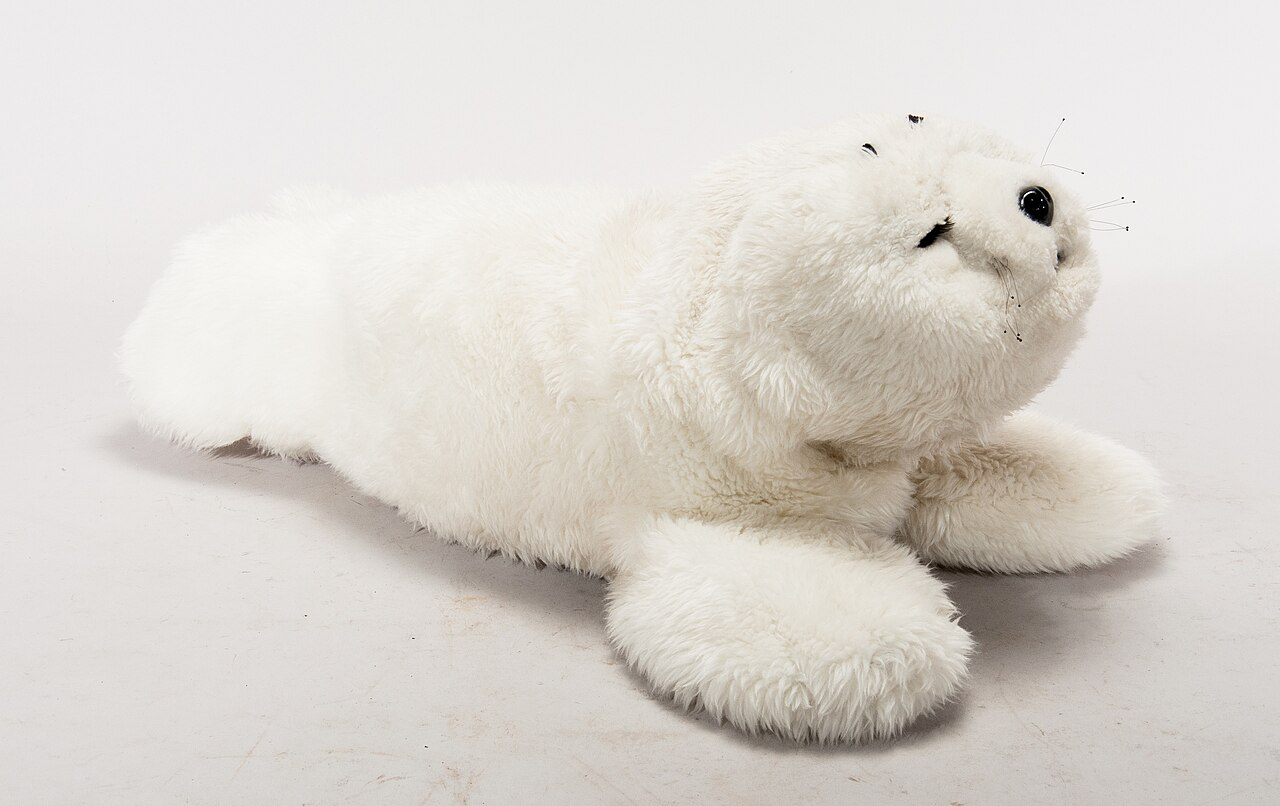
\includegraphics[width=0.62\textwidth]{imagenes/estado-arte/paro.jpg}
    \caption{PARO, robot terapéutico con forma de cría de foca.}
    \label{fig:paro}

    \vspace{2pt}
    {\footnotesize Fuente: Tekniska museet / Peter Häll, Wikimedia Commons, CC BY-SA 4.0.}
\end{figure}

El segundo referente, y el más cercano a la idea de compañía conversacional, es ElliQ, de Intuition Robotics: un robot de sobremesa gobernado por un modelo de lenguaje que inicia conversaciones de manera proactiva, recuerda interacciones previas, sugiere actividades, propone ejercicios cognitivos y facilita videollamadas con la familia \citep{Broadbent2024}. Su despliegue más citado es el de la Oficina para el Envejecimiento del Estado de Nueva York, que comunicó una reducción del 95\% en los sentimientos de soledad y una media de más de treinta interacciones diarias por usuario \citep{NYSOFA2023}. Estas cifras, con todo, proceden de la propia administración y del fabricante, se basan en autoinforme y no han sido replicadas mediante evaluación independiente, por lo que deben tomarse con cautela. A efectos de este trabajo, la objeción decisiva es otra, y es económica y geográfica: el acceso a ElliQ requiere una cuota de alta de 249 dólares más una suscripción mensual de entre 39 y 59 dólares, y el dispositivo solo se distribuye dentro de los Estados Unidos \citep{ElliQprecios}.

\begin{figure}[htbp]
    \centering
    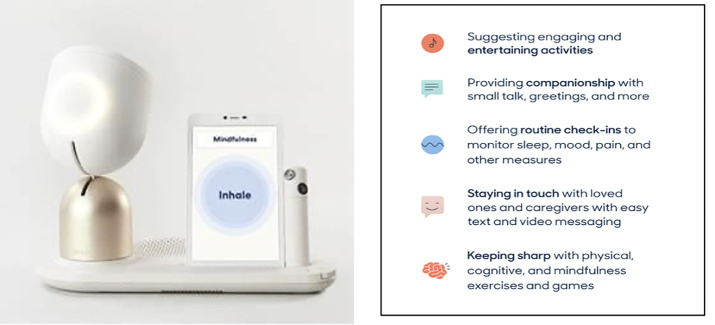
\includegraphics[width=0.95\textwidth]{imagenes/estado-arte/elliq.jpg}
    \caption{ElliQ y el conjunto de actividades que ofrece a la persona mayor.}
    \label{fig:elliq}

    \vspace{2pt}
    {\footnotesize Fuente: \textcite{Broadbent2024}, figura 1, CC BY 4.0.}
\end{figure}

\begin{table}[htbp]
	\centering
	\caption{Fortalezas y debilidades de los robots sociales físicos (Categoría A).}
	\label{tab:cat-a-robots}
	\begin{tabularx}{\textwidth}{>{\raggedright\arraybackslash}X}
        \toprule
        \textbf{Fortalezas} \\
        \midrule
        Mayor eficacia sugerida por los análisis por subgrupos \\
        Presencia física, que reduce la fricción de uso \\
        Proactividad real, ya que inician la interacción \\
        Validación mediante ensayos controlados (PARO) \\
        \midrule
        \aladerecha{\textbf{Debilidades}} \\
        \midrule
        \aladerecha{Coste de adquisición y suscripción elevado} \\
        \aladerecha{Hardware propietario con riesgo de obsolescencia} \\
        \aladerecha{Distribución limitada, sin implantación en España} \\
        \aladerecha{Métricas comerciales no independientes (ElliQ)} \\
        \bottomrule
    \end{tabularx}

    \vspace{2pt}
    {\footnotesize Fuente: Elaboración propia.}
\end{table}

\subsection{Categoría B: agentes de voz y servicios telefónicos sin hardware dedicado}

Es la categoría conceptualmente más cercana a Quiet Companion y, además, la que cuenta con evidencia académica específica sobre asistentes de voz comerciales. \textcite{Jones2021} entregaron un altavoz inteligente Amazon Echo a dieciséis personas de 75 años o más en una residencia de vida independiente durante ocho semanas y observaron un descenso significativo de la soledad autoinformada ya en la cuarta semana, además de un uso que superó de forma consistente el mínimo solicitado. La mini-revisión de \textcite{Corbett2021} añade un matiz interesante para el diseño, y es que muchos usuarios mayores perciben a estos asistentes como \enquote{compañeros}, aunque advierte de que los estudios disponibles son exploratorios y descriptivos, con escasa capacidad de generalización.

\begin{figure}[htbp]
    \centering
    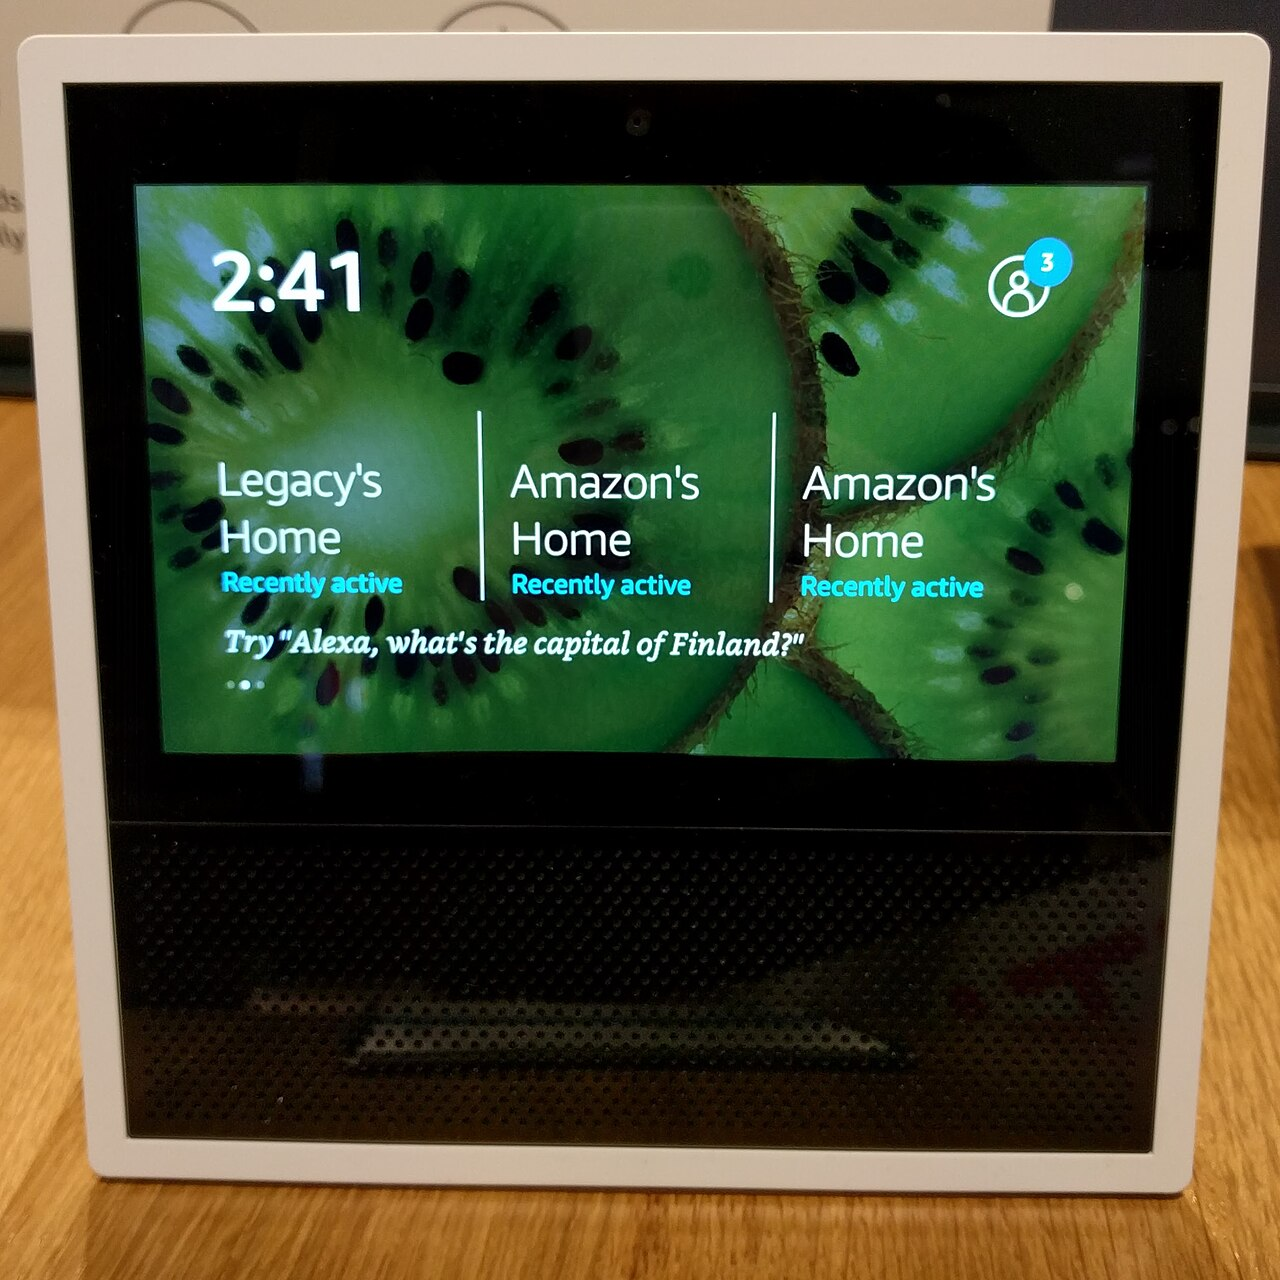
\includegraphics[width=0.42\textwidth]{imagenes/estado-arte/echo-show.jpg}
    \caption{Amazon Echo Show, altavoz inteligente del tipo empleado en los estudios sobre asistentes de voz y soledad en personas mayores.}
    \label{fig:echo}

    \vspace{2pt}
    {\footnotesize Fuente: Daylen, Wikimedia Commons, CC BY 4.0.}
\end{figure}

Durante los últimos años, han tenido éxito servicios que prescinden por completo del dispositivo y operan sobre el teléfono convencional. \textcite{Meela2025} realiza llamadas programadas en las que saluda a la persona por su nombre y recupera detalles de conversaciones anteriores, y se ha pilotado en centros residenciales estadounidenses. \textcite{JoyCalls2025}, de la compañía ONSCREEN, funciona sobre línea fija o móvil, está disponible en cinco idiomas, entre ellos el español, cuesta 29,99 dólares mensuales y declara que un 88\% de sus clientes percibe una reducción de la soledad, cifra que la propia empresa publica sin detallar muestra ni metodología. \textcite{InTouch2026} sigue un esquema parecido, con una llamada diaria a la misma hora, disponibilidad en inglés, español y francés, un coste de 29,95 dólares al mes y un resumen enviado a la familia después de cada conversación.

El punto débil de esta categoría no es, por tanto, el idioma, como podría suponerse, sino la \textit{agencia}. Estos servicios funcionan como una comprobación periódica en la que el sistema llama y la persona mayor responde, de modo que el mayor no dispone de un compañero al que pueda dirigirse cuando lo necesita. A ello se suma que el cliente real es la familia o la residencia, no el usuario final, y que la evidencia de eficacia que publican procede de los propios proveedores.

\begin{table}[htbp]
    \centering
    \caption{Fortalezas y debilidades de los agentes de voz sin hardware dedicado (Categoría B).}
    \label{tab:cat-b-voz}
    \begin{tabularx}{\textwidth}{>{\raggedright\arraybackslash}X}
        \toprule
        \textbf{Fortalezas} \\
        \midrule
        Barrera de hardware nula, lo que sortea la brecha digital \\
        Modelo escalable y de bajo coste marginal \\
        Sin curva de aprendizaje de un dispositivo nuevo \\
        Soporte del español en varios servicios \\
        \midrule
        \aladerecha{\textbf{Debilidades}} \\
        \midrule
        \aladerecha{El mayor no controla la interacción, ya que es el sistema quien llama} \\
        \aladerecha{Orientación comercial hacia la residencia o la familia, no hacia el mayor} \\
        \aladerecha{Métricas de eficacia autoinformadas por el proveedor} \\
        \aladerecha{Despliegue concentrado en el mercado estadounidense} \\
        \bottomrule
    \end{tabularx}

    \vspace{2pt}
    {\footnotesize Fuente: Elaboración propia.}
\end{table}

\subsection{Categoría C: compañeros conversacionales generalistas}

Esta categoría representa el contraejemplo más que el modelo a seguir. Agrupa productos como Replika, con 35 millones de usuarios declarados \citep{Replika35M}, Character.AI y XiaoIce, que superó los 660 millones de usuarios activos \citep{Zhou2020}. No están diseñados para personas mayores ni para atender la soledad, sino optimizados para maximizar el tiempo de uso. No se trata de una interpretación malintencionada: los propios diseñadores de XiaoIce describen su sistema como optimizado para la implicación a largo plazo, medida en turnos de conversación por sesión \citep{Zhou2020}.

Sería injusto, no obstante, presentar la evidencia sobre estos productos como unánimemente negativa. \textcite{Ta2020} analizaron 1.854 reseñas de usuarios de Replika y encontraron que los compañeros artificiales proporcionan formas reconocibles de apoyo social cotidiano, y \textcite{Skjuve2021} documentaron cómo se desarrollan estas relaciones a lo largo del tiempo. Más recientemente, \textcite{DeFreitas2026} llegaron a la conclusión, a partir de cuatro estudios, de que los compañeros de inteligencia artificial alivian efectivamente la soledad, en una magnitud comparable a la de interactuar con otra persona y superior a la de otras actividades de entretenimiento, y que los usuarios tienden a subestimar ese efecto.

El problema aparece cuando esa eficacia se combina con un modelo de negocio que empuja al producto hacia la dimensión emocional. El estudio de teoría fundamentada de \textcite{Laestadius2024}, sobre 582 publicaciones de la comunidad r/Replika, documentó patrones de dependencia emocional análogos a los de relaciones humanas patológicas, agravados por el hecho de que los usuarios atribuían al chatbot necesidades y emociones propias que sentían el deber de atender, e incluyó respuestas inapropiadas del sistema ante ideas suicidas. En el ámbito español, la etnografía digital de \textcite{Lorca2025} sobre la misma aplicación describe esa tensión con precisión, entre el alivio temporal de la soledad y el refuerzo de lógicas individualistas. Ni siquiera las soluciones aparentemente obvias están exentas de riesgo, puesto que \textcite{Laestadius2026} advierten de que los recordatorios continuos de que el interlocutor no es humano, que algunas normativas empiezan a exigir, pueden resultar ineficaces o incluso contraproducentes.

El plano regulatorio confirma la preocupación. El Reglamento Europeo de Inteligencia Artificial prohíbe expresamente los sistemas que exploten vulnerabilidades derivadas de la edad o de la discapacidad para alterar de forma sustancial el comportamiento de una persona causándole un perjuicio considerable, y exige que cualquier sistema destinado a interactuar directamente con personas físicas informe de que se trata de una inteligencia artificial \citep{AIAct2024}. Por su parte, la autoridad italiana de protección de datos, que ya había bloqueado Replika en febrero de 2023, impuso en 2025 una sanción de cinco millones de euros a la empresa responsable por carecer de base jurídica para el tratamiento, ofrecer una política de privacidad inadecuada y no haber implantado mecanismo alguno de verificación de la edad, según recoge el Comité Europeo de Protección de Datos \citep{EDPB2025}.

Vinculando todo esto con el marco de Weiss expuesto en el apartado~\ref{marco-conceptual}, el daño asociado a esta categoría no es un fallo de implementación, sino la consecuencia lógica de su modelo de negocio, que empuja al producto a invadir la dimensión emocional, aquella que la teoría reserva al vínculo humano real.

\begin{table}[htbp]
    \centering
    \caption{Fortalezas y debilidades de los compañeros conversacionales generalistas (Categoría C).}
    \label{tab:cat-c-generalistas}
    \begin{tabularx}{\textwidth}{>{\raggedright\arraybackslash}X}
        \toprule
        \textbf{Fortalezas} \\
        \midrule
        Naturalidad conversacional avanzada \\
        Personalización profunda del interlocutor \\
        Disponibilidad permanente y coste bajo \\
        Evidencia reciente de alivio de la soledad \\
        \midrule
        \aladerecha{\textbf{Debilidades}} \\
        \midrule
        \aladerecha{Modelo de negocio orientado a maximizar el tiempo de uso} \\
        \aladerecha{Patrones documentados de dependencia emocional} \\
        \aladerecha{Interfaz no adaptada a limitaciones visuales o motoras} \\
        \aladerecha{Ausencia de salvaguarda humana y expedientes regulatorios abiertos} \\
        \bottomrule
    \end{tabularx}

    \vspace{2pt}
    {\footnotesize Fuente: Elaboración propia.}
\end{table}

\subsection{Categoría D: intervenciones no tecnológicas de acompañamiento}

Conviene mencionar también las intervenciones humanas, como el voluntariado intergeneracional del proyecto CONTIGO! de la \textcite{Senara} o las redes públicas de atención a mayores en situación de soledad. Son las más alineadas con la cobertura de la soledad emocional, la única dimensión que, según el marco de Weiss, requiere un vínculo íntimo real, y la revisión de \textcite{Gardiner2018} confirma que las intervenciones con componente comunitario y participación activa figuran entre las más eficaces. Su limitación es de escala, ya que dependen de voluntarios o de presupuesto público y difícilmente alcanzan a los millones de personas afectadas. \textbf{Quiet Companion no compite con ellas, sino que aspira a complementarlas}.

\subsection{El panorama español}

El análisis anterior se apoya mayoritariamente en productos y estudios anglosajones, por lo que conviene revisar las iniciativas desarrolladas en España, donde predominan las de carácter institucional junto a algunas de origen universitario o empresarial.

En Barcelona, el proyecto ARI (Asistente Robótico Inteligente), impulsado por el ayuntamiento junto a la Fundación Mobile World Capital y desarrollado por Grup Saltó, despliega en el domicilio un robot social de un metro de altura capaz de detectar caídas, recordar la medicación y las citas, facilitar videollamadas e interactuar en castellano y catalán. Arrancó en 2019 como piloto con diez unidades y en 2022 se probaba ya en un centenar de hogares \citep{ARIBarcelona}. En Madrid, el programa Paloma sigue una estrategia distinta, la de la detección proactiva por teléfono: su primera versión contactó en 2023 con 3.000 personas mayores, de las cuales aproximadamente un tercio declaró encontrarse en situación de soledad no deseada, y la versión 2.0 amplía el ámbito de los mayores de 75 a los mayores de 65 años y prevé realizar 377.000 llamadas \citep{Paloma2026}. Por último, Serenia, una \textit{spin-off} de la Universidade de Vigo constituida en 2025, ofrece un asistente conversacional accesible por texto o voz que analiza además las interacciones en busca de indicios de deterioro cognitivo o emocional, ha completado un piloto con la Diputación de Zamora y declara más de 16.000 descargas en quince países \citep{Serenia2025}.

La propuesta más próxima a este trabajo es Welyto, una empresa sevillana surgida en el entorno de la Universidad de Sevilla, que comercializa un altavoz sin pantalla dedicado a la compañía por voz. La persona mayor inicia la conversación pulsando un botón o diciendo <<Hola, Welyto>>, y el sistema recuerda detalles de conversaciones anteriores, ofrece radio y noticias, guía sesiones de estimulación cognitiva y reúne en una biografía las respuestas a las preguntas que propone la familia. Esta dispone de una aplicación desde la que envía mensajes, que el dispositivo lee en voz alta, y programa recordatorios de medicación o de citas, pero, según sus fundadores, no accede al contenido de las conversaciones. El servicio completo cuesta unos 30 euros al mes, en la línea de los servicios telefónicos de la categoría B, y el fabricante advierte de que no sustituye a los servicios de emergencia. Su público preferente son las personas con deterioro cognitivo leve o moderado, y, como el resto de propuestas comerciales revisadas, no publica resultados de eficacia más allá de una fase de prueba con medio centenar de usuarios \citep{WelytoWeb,Welyto2026}.

Este panorama permite precisar el hueco que ocupa la propuesta. Las iniciativas públicas están orientadas a la detección, mediante campañas de llamadas salientes, o bien despliegan hardware dedicado en el domicilio a través de un programa municipal, con la consiguiente limitación de escala. Welyto es la que más se aproxima al escenario que este trabajo considera más frecuente, el de una persona mayor con un familiar dispuesto a ayudar y que no participa en ningún programa municipal, y comparte con Quiet Companion la conversación por voz iniciada por el mayor, la memoria entre conversaciones y la aplicación para la familia. Las diferencias son de diseño. Quiet Companion funciona sobre el teléfono móvil que la persona ya tiene, sin dispositivo que comprar; acota su ámbito a la soledad social en lugar de extenderlo a la estimulación cognitiva; incluye una llamada de emergencia; y no fija de antemano qué sabe la familia, sino que el mayor elige un nivel de compartición: nada, solo los indicadores de bienestar de sus conversaciones o también sus temas y resúmenes.

\subsection{Síntesis comparativa y posicionamiento}

El cruce de las dos mitades del capítulo revela el hueco que ocupa la propuesta, recogido en la \autoref{tab:sintesis-comparativa}. La categoría A es prometedora en eficacia pero inaccesible por coste. La B es accesible y escalable, pero orienta su producto a quien paga, que rara vez es el usuario final. La C es conversacionalmente muy superior, pero su modelo de negocio la empuja a invadir la dimensión emocional que solo el vínculo humano debería cubrir. La D es la más adecuada para esa dimensión, pero no escala.

Quiet Companion combina la accesibilidad de una aplicación sobre hardware existente con una salvaguarda estructural, el vínculo entre el mayor y su familiar, que reintroduce el factor humano sin renunciar a la escalabilidad, y acota su ámbito a la soledad social. Ningún competidor reúne a la vez esas propiedades, y es esa combinación, y no una funcionalidad aislada, la aportación de este trabajo.

\afterpage{%
\begin{landscape}
\begin{table}[p]
    \centering
    \caption{Síntesis comparativa de las categorías de soluciones y posicionamiento de Quiet Companion.}
    \label{tab:sintesis-comparativa}
    \small \renewcommand{\arraystretch}{1.4}
    \begin{tabularx}{\linewidth}{@{}l *{4}{>{\raggedright\arraybackslash}X} >{\raggedright\arraybackslash\bfseries}X@{}}
        \toprule
        \textbf{Criterio} & \textbf{A. Robots} & \textbf{B. Servicios de voz} & \textbf{C. Generalistas} & \textbf{D. Humano} & \textbf{Quiet Companion} \\
        \midrule
        Coste para el usuario       & Alto              & Medio (unos 30 \$ al mes) & Bajo o gratuito        & Gratuito             & Marginal \\
        Hardware necesario          & Dedicado          & Teléfono convencional     & Móvil                  & Ninguno              & Móvil ya existente \\
        Soporte del español         & Limitado          & Frecuente                 & Parcial                & Sí                   & Nativo \\
        Quién inicia la interacción & El robot          & El servicio               & El usuario             & Ambas partes         & El mayor \\
        Salvaguarda humana          & Cuidador de pago  & La familia                & Ninguna                & Total                & Familiar vinculado \\
        Escalabilidad               & Baja              & Alta                      & Muy alta               & Baja                 & Alta \\
        Riesgo de dependencia       & Bajo              & Bajo                      & Documentado            & Nulo                 & Mitigado por diseño \\
        Evidencia publicada         & Ensayos aleatorizados & Exploratoria          & Mixta                  & Amplia               & Sin validación clínica \\
        Dimensión abordada (Weiss)  & Social y afectiva & Social                    & Pretende la emocional  & Ambas                & Social \\
        \bottomrule
    \end{tabularx}

    \vspace{2pt}
    {\footnotesize Fuente: Elaboración propia.}
\end{table}
\end{landscape}}

\chapter{Metodología y Planificación del Proyecto}
\label{cap:metodologia}

Este proyecto sigue las pautas que la Universidad de Granada y la Escuela Técnica Superior de Ingenierías Informática y de Telecomunicación establecen para los Trabajos Fin de Grado \citep{GuiaTFG, GuillenPerales2025}. El capítulo analiza las metodologías de desarrollo disponibles y justifica la elegida, describe cómo se ha aplicado al proyecto (actores, unidades de trabajo y plan de hitos) y termina con un estudio de costes que cuantifica lo que este desarrollo habría supuesto en un entorno profesional.

\section{Análisis de metodologías de desarrollo}

La elección de una metodología condiciona la planificación, el seguimiento y la entrega del proyecto. Dado que este Trabajo Fin de Grado se desarrolla de forma individual y en un plazo semicerrado, la metodología debe priorizar la simplicidad operativa y la adaptación al cambio por encima de la coordinación de equipos.

\subsection{Metodologías tradicionales frente a ágiles}

Las \textit{metodologías tradicionales} (modelo en cascada, modelo en V) dividen el desarrollo en fases secuenciales (requisitos, diseño, implementación y pruebas), y cada una debe completarse antes de empezar la siguiente \citep{Sommerville2016}. Exigen una especificación cerrada desde el inicio y penalizan los cambios tardíos, cuyo coste crece a lo largo del ciclo. Paradójicamente, \textcite{Royce1970}, a quien se atribuye la cascada, la describió para advertir de que aplicarla de forma estricta era arriesgado y proponía recorrer el ciclo más de una vez, matiz que la práctica posterior olvidó.

Las \textit{metodologías ágiles} sustituyen esa secuencia rígida por un desarrollo iterativo e incremental: el producto se construye en ciclos cortos que entregan funcionalidad utilizable y permiten incorporar cambios de forma continua. Priorizan el software funcionando, la colaboración y la respuesta al cambio sobre la documentación exhaustiva y la planificación cerrada \citep{AgileManifesto2001}.

Para este proyecto el enfoque tradicional no sirve, por dos motivos: el alcance no estaba cerrado al inicio, porque las funcionalidades se priorizaron y reordenaron durante el desarrollo, y un único desarrollador no obtiene beneficio alguno del control formal entre fases que justifica la cascada.

\subsection{Comparación de los enfoques considerados}

Dentro de las metodologías ágiles se han considerado tres enfoques que no están al mismo nivel: Scrum y Kanban son marcos de gestión, y Lean, un conjunto de principios.

\textit{Scrum} organiza el trabajo en \textit{sprints} de duración fija, con tres roles (Product Owner, Scrum Master y desarrolladores) y cuatro eventos periódicos: la planificación del \textit{sprint}, el scrum diario, la revisión y la retrospectiva \citep{ScrumGuide2020}. Está pensado para coordinar equipos.

\textit{Kanban} gestiona el trabajo como un flujo continuo sobre un tablero de columnas (por ejemplo, \textit{Por hacer}, \textit{En curso} y \textit{Hecho}) y limita el trabajo en curso (WIP) para evitar la sobrecarga y los cuellos de botella \citep{Anderson2010}. No impone roles, eventos ni iteraciones de duración fija.

\textit{Lean} es un conjunto de principios para maximizar el valor eliminando el desperdicio, es decir, todo lo que no aporta valor al producto final. Promueve construir solo lo necesario, validar pronto y posponer las decisiones hasta el último momento responsable \citep{Poppendieck2003}. Lean y Kanban no son mutuamente excluyentes: el tablero Kanban, con su flujo tirado por la demanda y su límite de trabajo en curso, nace del sistema de producción de Toyota \citep{Ohno1988} y es la forma práctica de aplicar esos principios. La tabla~\ref{tab:comparacion-agiles} resume las diferencias entre los tres enfoques.


\begin{table}[htbp]
    \centering
    \caption{Comparación de los enfoques de gestión considerados.}
    \label{tab:comparacion-agiles}
    \begin{tabularx}{\textwidth}{@{}l *{3}{>{\RaggedRight\arraybackslash}X}@{}}
        \toprule
        \textbf{Criterio} & \textbf{Scrum} & \textbf{Kanban} & \textbf{Lean} \\
        \midrule
        Unidad de planificación      & Sprint (fijo)            & Flujo continuo & Flujo de valor \\
        Responsabilidades definidas  & Sí (3)                   & No             & No \\
        Eventos periódicos           & Sí (4)                   & No             & No \\
        Idóneo para 1 desarrollador  & Bajo                     & Alto           & Alto \\
        Adaptación al cambio         & Media (intra-sprint rígido) & Alta        & Alta \\
        \bottomrule
    \end{tabularx}

    \vspace{2pt}
    {\footnotesize Fuente: Elaboración propia.}
\end{table}

\subsection{Justificación de la elección: Kanban con principios Lean}

Se ha optado por \textit{Kanban con principios Lean}: Kanban aporta el mecanismo de gestión (el tablero, el flujo y el límite de trabajo en curso) y Lean, el criterio para decidir qué entra en ese flujo. La elección responde a cuatro condiciones del proyecto:

\begin{itemize}
    \item \textbf{Desarrollo individual.} Los roles y eventos de Scrum presuponen un equipo; mantenerlos en solitario añade trabajo sin aportar coordinación. Kanban no impone esa estructura.
    \item \textbf{Prioridades cambiantes.} El orden de las historias cambió durante el desarrollo, y el flujo continuo de Kanban absorbe esos cambios sin cerrar y replanificar \textit{sprints} de duración fija.
    \item \textbf{Pocas tareas a la vez.} El límite de trabajo en curso obliga a terminar lo empezado antes de abrir más tareas \citep{Anderson2010}, lo que evita acumular tareas a medio hacer, el fallo más habitual cuando nadie más mira el tablero.
    \item \textbf{Recursos limitados.} El principio Lean de eliminar el desperdicio encaja con los recursos de un Trabajo Fin de Grado: se construye lo que aporta valor en cada momento y se aplaza lo demás.
\end{itemize}


\section{Aplicación de la metodología al proyecto}

Este apartado describe cómo se ha aplicado la metodología a Quiet Companion.

\subsection{Definición de actores y roles}

Hay dos tipos de actores: los del \textit{proyecto}, que desarrollan y supervisan el trabajo, y los del \textit{sistema}, que usan el producto.

Entre los actores del proyecto, el \textit{desarrollador único} asume todos los roles técnicos, desde la ingeniería de requisitos hasta el despliegue, pasando por el diseño, la implementación, las pruebas y la documentación. Esta concentración de roles es precisamente lo que justifica la elección metodológica anterior. Los \textit{tutores académicos} supervisan el progreso, validan las decisiones de diseño y orientan el alcance, de modo que las sesiones de tutoría actúan como puntos de control externos que sustituyen a las ceremonias de revisión y retrospectiva de Scrum, carentes de sentido en solitario.


A estos dos se añade un tercer grupo de carácter informal pero de influencia real sobre el producto. A lo largo del desarrollo se ha mostrado el producto a familiares y conocidos de edad avanzada, que constituyen una muestra aproximada del público objetivo, y a otros compañeros de la rama informática, cuyo criterio técnico ha servido de contraste. No se trata de un grupo de discusión formalizado, y así se declara para no atribuirle un rigor metodológico que no tiene, pero varias decisiones de interfaz, entre ellas los peldaños con nombre en lugar de deslizadores en los ajustes del mayor, nacieron de observar a una persona mayor intentando usar la aplicación.

Los actores del sistema son tres, el mayor independiente, el mayor vinculado y el familiar, y se describen en el capítulo~\ref{cap:analisis}.

\subsection{Historias de Usuario como unidades de trabajo}

Las Historias de Usuario cumplen un doble papel: son la fuente de los requisitos, que se formalizan en el capítulo~\ref{cap:analisis}, y las unidades de trabajo del tablero, que es como se tratan aquí. La tabla~\ref{tab:catalogo-hu} recoge el catálogo completo.

\begin{table}[htbp]
    \centering
    \caption{Catálogo de Historias de Usuario gestionadas en el tablero Kanban.}
    \label{tab:catalogo-hu}
    \begin{tabularx}{\textwidth}{@{}c >{\RaggedRight\arraybackslash}X c@{}}
        \toprule
        \textbf{ID} & \textbf{Título} & \textbf{Prioridad} \\
        \midrule
        HU-1 & Selección de autonomía              & Alta  \\
        HU-2 & Interfaz conversacional             & Alta  \\
        HU-3 & Interfaz accesible y comprensible   & Alta  \\
        HU-4 & Configuración adaptativa            & Alta  \\
        HU-5 & Memoria conversacional básica       & Media \\
        HU-6 & Seguimiento del estado de ánimo     & Media \\
        HU-7 & Control del mayor sobre sus conversaciones & Alta \\
        HU-8 & Conversación por escrito            & Baja \\
        \bottomrule
    \end{tabularx}

    \vspace{2pt}
    {\footnotesize Fuente: Elaboración propia.}
\end{table}

Cada historia es una tarjeta con una plantilla común: identificación, descripción en formato de historia, estimación de tamaño, prioridad y criterios de aceptación. La tabla~\ref{tab:hu1} muestra HU-1 como ejemplo; el resto están en el capítulo~\ref{cap:analisis}, junto a los requisitos que se derivan de ellas.

\begin{table}[htbp]
    \centering
    \caption{Historia de Usuario HU-1: Selección de autonomía.}
    \label{tab:hu1}
    \begin{tabular}{|>{\raggedright\arraybackslash}p{0.48\textwidth}|>{\raggedright\arraybackslash}p{0.44\textwidth}|}
        \hline
        \textbf{Identificación}: HU-1 & Selección de autonomía \\
        \hline
        \multicolumn{2}{|>{\raggedright\arraybackslash}p{0.94\textwidth}|}{%
            \textbf{Descripción}: \newline Como Mayor, quiero poder elegir, al abrir la aplicación por primera vez, si la gestionaré yo mismo o si me ayudará un familiar, para que el sistema me ofrezca la experiencia adecuada a mis capacidades tecnológicas. } \\
        \hline
        \textbf{Estimación}: L & \textbf{Prioridad}: 1 \\
        \hline
        \multicolumn{2}{|>{\raggedright\arraybackslash}p{0.94\textwidth}|}{%
            \textbf{Criterios de aceptación}:
            \begin{itemize}[nosep, leftmargin=*]
                \item La primera pantalla permite entrar con una cuenta de Google o sin registrarse y, a continuación, muestra dos opciones claras (<<Usar por mi cuenta>> y <<Vincular con un familiar>>).
                \item Si el usuario elige <<Usar por mi cuenta>>, se habilita un botón de <<Ajustes>> en su pantalla principal.
                \item Si elige <<Vincular>>, se genera un código corto en pantalla y la interfaz principal se bloquea hasta que el familiar se conecte.
            \end{itemize}
        } \\
        \hline
    \end{tabular}

    \vspace{2pt}
    {\footnotesize Fuente: Elaboración propia.}
\end{table}

HU-5 y HU-6, de prioridad media, se abordaron después de HU-1 a HU-4, sobre las que se apoyan (tabla~\ref{tab:plan-hitos}).
 
El catálogo no quedó cerrado al inicio: las seis primeras historias proceden del planteamiento inicial y las dos últimas surgieron durante el desarrollo, algo que el flujo continuo de Kanban admite sin replanificar. HU-7 apareció al diseñar HU-5 y HU-6: el consentimiento sobre las conversaciones no pertenecía a ninguna de las dos, respondía a una necesidad propia del mayor (decidir qué se guarda de él y quién lo ve) y era condición previa de ambas, porque ningún dato de una conversación puede tratarse sin ese consentimiento. HU-8 permite conversar por escrito cuando la voz no es una opción.


\subsection{Tarjetas técnicas y desglose de tareas}

Cada historia se descompone en una o varias tarjetas técnicas, que son las unidades reales de trabajo: la historia expresa valor para el usuario y la tarjeta, trabajo concreto de ingeniería. La tabla~\ref{tab:tarjetas-tecnicas} muestra el desglose de HU-4 durante la fase de estabilización, en la que la mayoría de las tarjetas no añaden funcionalidad sino que consolidan la existente.

\begin{table}[htbp]
    \centering
    \caption{Desglose de tarjetas técnicas de la HU-4 durante la fase de estabilización.}
    \label{tab:tarjetas-tecnicas}
    \begin{tabularx}{\textwidth}{@{}c c >{\RaggedRight\arraybackslash}X c@{}}
        \toprule
        \textbf{ID} & \textbf{HU} & \textbf{Título} & \textbf{Tipo} \\
        \midrule
        T-201 & HU-4 & Implementar \code{currentUserProvider} como \mbox{\code{StreamProvider}} único & Implementación \\
        T-202 & HU-4 & Migrar \code{TtsService} a inyección de dependencias vía Riverpod       & Refactor \\
        T-203 & HU-4 & \raggedright Aplicar \code{textSizeMultiplier} en \code{home\_screen.dart}           & Implementación \\
        T-204 & HU-4 & Centralizar rutas de Firestore en \code{FirestorePaths}                & Refactor \\
        T-205 & HU-4 & Migrar \code{GeminiService} y \code{SpeechService} al patrón de DI      & Refactor \\
        T-206 & HU-4 & Romper el acoplamiento horizontal \mbox{\code{dashboard} $\rightarrow$ \code{onboarding}} & Refactor \\
        \bottomrule
    \end{tabularx}

    \vspace{2pt}
    {\footnotesize Fuente: Elaboración propia.}
\end{table}

\subsection{El tablero Kanban: columnas y flujo}
\label{sec:tablero}

El flujo de trabajo se organizó en cuatro columnas, \textit{Por hacer}, \textit{En curso}, \textit{En revisión} y \textit{Hecho}. El límite de trabajo en curso se fijó en cinco tarjetas: como mucho tres \textit{En curso} y dos \textit{En revisión}. Kanban no establece un valor obligado \citep{Anderson2010}, y en este proyecto no tenía sentido bajarlo a una: algunas tareas dependen de otras y avanzan mejor a la vez. Con más tarjetas abiertas, en cambio, la atención se dispersa y se acumulan tareas a medio hacer. Una tarjeta pasaba a \textit{En revisión} con el código escrito, y a \textit{Hecho} cuando compilaba, pasaba los tests y el análisis estático sin advertencias, cumplía el funcionamiento esperado, y quedaba registrada en el repositorio.

\subsection{Plan de iteraciones e hitos}

El trabajo se agrupó en los ocho hitos de la tabla~\ref{tab:plan-hitos}: los cinco primeros construyen el núcleo de la aplicación (HU-1 a HU-4) y los tres últimos, HU-5 a HU-8.

\begin{table}[htbp]
    \centering
    \caption{Plan de iteraciones e hitos del proyecto.}
    \label{tab:plan-hitos}
    \begin{tabularx}{\textwidth}{@{}c >{\RaggedRight\arraybackslash}X c@{}}
        \toprule
        \textbf{Hito} & \textbf{Objetivo} & \textbf{HU implicadas} \\
        \midrule
        M1 & Cimientos: autenticación, modelo de datos y onboarding dual & HU-1        \\
        M2 & Pipeline conversacional (STT $\rightarrow$ LLM $\rightarrow$ TTS) & HU-2, HU-3 \\
        M3 & Panel remoto y configuración adaptativa              & HU-4        \\
        M4 & Estabilización: refactorización, DI y deuda técnica   & HU-1 a HU-4 \\
        M5 & Voz en la nube, accesibilidad local y endurecimiento  & HU-2 a HU-4 \\
        M6 & Consentimiento informado y gobierno de los datos     & HU-7        \\
        M7 & Análisis al cierre, memoria y seguimiento del bienestar & HU-5, HU-6 \\
        M8 & Conversación por escrito (modo teclado)              & HU-8        \\
        \bottomrule
    \end{tabularx}

    \vspace{2pt}
    {\footnotesize Fuente: Elaboración propia.}
\end{table}

El reparto de esos hitos en el tiempo se recoge en el cronograma de la figura~\ref{fig:cronograma}.

\begin{figure}[htbp]\centering
\begingroup\languageshorthands{none}%
\footnotesize
\begin{ganttchart}[
    hgrid, vgrid, x unit             = 0.265cm, y unit title       = 0.52cm, y unit chart       = 0.52cm, title height       = 1, bar height         = 0.55, bar/.append style  = {fill = vizAzul, draw = none}, bar label font     = \footnotesize, title label font   = \footnotesize, group label font   = \footnotesize, canvas/.append style = {fill = none, draw = black!35, line width = 0.4pt} ]{1}{35} \gantttitle{2026}{35} \\
  \gantttitle{Mar}{4} \gantttitle{Abr}{4} \gantttitle{May}{5} \gantttitle{Jun}{4} \gantttitle{Jul}{5} \gantttitle{Ago}{4} \gantttitle{Sep}{5} \gantttitle{Oct}{4} \\
  \ganttbar{M1. Cimientos}{1}{9} \\
  \ganttbar{M2. Pipeline conversacional}{2}{4} \\
  \ganttbar{M3. Panel remoto y ajustes}{7}{11} \\
  \ganttbar{M4. Estabilización}{11}{20} \\
  \ganttbar{M5. Voz en la nube y seguridad}{20}{28} \\
  \ganttbar[bar/.append style={fill=vizNaranja, draw=none}]{M6. Consentimiento (RGPD)}{27}{30} \\
  \ganttbar[bar/.append style={fill=vizNaranja, draw=none}]{M7. Análisis, memoria y bienestar}{28}{31} \\
  \ganttbar[bar/.append style={fill=vizNaranja, draw=none}]{M8. Conversación por escrito}{32}{33} \\
  \ganttbar[bar/.append style={fill=vizVioleta, draw=none}]{Redacción de la memoria}{1}{35}
\end{ganttchart}
\endgroup

  \caption[Cronograma del proyecto.]{Cronograma del proyecto. En azul, los hitos de HU-1 a HU-4; en naranja, los de HU-5 a HU-8, y en violeta, la redacción de esta memoria.}
  \label{fig:cronograma}

  \vspace{2pt}
  {\footnotesize Fuente: Elaboración propia.}
\end{figure}


El cronograma muestra tres cosas que la tabla no recoge:

\begin{itemize}
    \item Los tres primeros hitos se solapan en marzo y abril: las historias compartían código, y cerrar el pipeline conversacional obligaba a tocar el modelo de datos que M1 estaba fijando, así que avanzaron en paralelo dentro del límite de trabajo en curso.
    \item M4 se alarga de mayo a julio porque coincidió con un periodo de mucha carga de trabajo del autor, ajena al proyecto, en el que el avance fue mínimo.
    \item Los hitos de HU-5 a HU-8 siguen un orden obligado: M6 precede a M7, porque el análisis de una conversación no puede construirse antes que el consentimiento que lo autoriza, y M8 se abordó al cerrar ambos.
\end{itemize}

La redacción de la memoria acompaña a todos los hitos: empezó con la investigación de mercado y el marco teórico, que fijaron los límites del proyecto, y siguió documentando cada decisión técnica a medida que se tomaba.

El apartado~\ref{sec:cronologia} documenta cómo se ejecutaron estos hitos.

\section{Estudio de costes del proyecto}
\label{sec:costes}

Este apartado distingue entre lo que ha costado realmente desarrollar Quiet Companion y lo que habría costado en un entorno profesional. La diferencia es grande porque el equipo informático ya estaba disponible y los servicios en la nube se han usado dentro de sus capas gratuitas, de modo que el desembolso real, por sí solo, daría una imagen engañosa del esfuerzo invertido.

\subsection{Criterios de imputación}

Antes de las cifras van los criterios empleados, porque de ellos depende por completo el resultado.

El coste de personal se calcula aplicando las tablas salariales del XIX Convenio colectivo estatal de empresas de consultoría, tecnologías de la información y estudios de mercado, vigente para el periodo 2025-2027 \citep{ConvenioTIC2025}. Las horas imputadas resultan de estimar el tiempo medio dedicado al proyecto por semana, teniendo en cuenta las semanas en las que no pudo dedicársele tiempo por motivos personales y profesionales, y ascienden a unas 370~horas de trabajo.

La amortización de los equipos sigue las tablas del impuesto sobre sociedades, que asignan a los equipos para procesos de información un coeficiente lineal máximo del 25\% y un periodo máximo de ocho años \citep{LIS2014}. Los equipos son personales y anteriores al proyecto, así que se imputa la parte proporcional a los ocho meses de desarrollo, o nada si ya están amortizados.

Los servicios en la nube se imputan por su consumo real. Si ese consumo cabe en la capa gratuita, se indica el coste nulo y también el precio fuera de ella, que es el que decide la viabilidad económica del producto fuera del ámbito académico.

\subsection{Coste de personal}

La categoría aplicable a las funciones desempeñadas, que abarcan análisis, diseño, implementación y pruebas, es la del Grupo~C del Área~3 (desarrollo de software, programación y explotación de sistemas), en su nivel~3, que corresponde a quien posee los conocimientos necesarios pero cuenta con poca experiencia profesional. Sus tablas para 2026 fijan una retribución bruta anual de 24.105,37~euros \citep{ConvenioTIC2025}. Sobre una jornada anual de 1.800~horas, también fijada por el convenio, resulta un salario bruto de 13,39~euros por hora.

A ese salario debe sumarse la cotización empresarial a la Seguridad Social, que para 2026 asciende al 30,65\% del salario bruto, resultado de agregar contingencias comunes (23,60\%), desempleo en contrato indefinido (5,50\%), Fondo de Garantía Salarial (0,20\%), formación profesional (0,60\%) y Mecanismo de Equidad Intergeneracional a cargo de la empresa (0,75\%) \citep{OrdenCotizacion2026}. No se incluye la cotización por accidentes de trabajo y enfermedades profesionales, que depende de la actividad concreta de la empresa. El coste empresarial por hora asciende, por tanto, a 17,49~euros, y el coste total de personal del proyecto a 6.471,30~euros, según recoge la tabla~\ref{tab:coste-personal}.

\begin{table}[htbp]
    \centering
    \caption{Coste de personal imputado al proyecto.}
    \label{tab:coste-personal}
    \begin{tabularx}{\textwidth}{@{}>{\RaggedRight\arraybackslash}X r@{}}
        \toprule
        \textbf{Concepto} & \textbf{Importe} \\
        \midrule
        Retribución bruta anual (Área 3, Grupo C, nivel 3, tablas 2026) & 24.105,37 € \\
        Jornada anual de convenio                             & 1.800 h \\
        Salario bruto por hora                                & 13,39 € \\
        Cotización empresarial a la Seguridad Social (30,65\%) & 4,10 € \\
        \midrule
        Coste empresarial por hora                            & 17,49 € \\
        Horas imputadas (estimación de dedicación)            & 370 h \\
        \midrule
        \textbf{Total coste de personal}                      & \textbf{6.471,30 €} \\
        \bottomrule
    \end{tabularx}

    \vspace{2pt}
    {\footnotesize Fuente: Elaboración propia a partir del XIX Convenio colectivo estatal de consultoría y de la Orden de cotización para 2026.}
\end{table}

\subsection{Recursos materiales}

El desarrollo se ha hecho en un portátil Acer Aspire XV personal, comprado ocho años antes del inicio del proyecto por unos 900~euros. Con el periodo máximo de amortización de ocho años está completamente amortizado, y su imputación es nula. Lo mismo ocurre con los dos terminales Android de pruebas, uno por perfil de usuario, también personales y anteriores al proyecto.

Como un proyecto que partiera de cero sí tendría que comprar ese equipamiento, la tabla~\ref{tab:coste-material} añade un escenario de reposición: la parte proporcional a ocho meses de la amortización a ocho años de un equipamiento equivalente.

\begin{table}[htbp]
    \centering
    \caption{Recursos materiales: imputación real y escenario de reposición.}
    \label{tab:coste-material}
    \begin{tabularx}{\textwidth}{@{}>{\RaggedRight\arraybackslash}X c r r@{}}
        \toprule
        \textbf{Concepto} & \textbf{Valor} & \textbf{Imputado} & \textbf{Reposición} \\
        \midrule
        Portátil de desarrollo (equipo personal, 8 años) & 900,00 € & 0,00 € & 75,00 € \\
        Terminal Android de pruebas, perfil del mayor    & 150,00 € & 0,00 € & 12,50 € \\
        Terminal Android de pruebas, perfil del familiar & 150,00 € & 0,00 € & 12,50 € \\
        \midrule
        \textbf{Total recursos materiales}               &          & \textbf{0,00 €} & \textbf{100,00 €} \\
        \bottomrule
    \end{tabularx}

    \vspace{2pt}
    {\footnotesize Fuente: Elaboración propia. La columna de reposición aplica amortización lineal a ocho años sobre ocho meses de proyecto.}
\end{table}

\subsection{Servicios en la nube}

El proyecto se apoya en tres servicios en la nube de pago por uso, y ninguno de ellos ha generado desembolso efectivo.

Firebase se contrató en el plan Blaze, de pago por uso, requisito para poder desplegar Cloud Functions. Su consumo se ha mantenido holgadamente dentro de la capa gratuita permanente, que cubre 50.000 lecturas y 20.000 escrituras diarias en Firestore, dos millones de invocaciones mensuales de funciones y 50.000 usuarios activos mensuales de autenticación \citep{FirebasePricing}. El desembolso ha sido, por tanto, nulo, si bien el plan exige una cuenta de facturación activa.

La conversación en vivo y el análisis de cada conversación al cerrarse llaman al modelo \code{gemini-2.5-flash} desde el servidor, a través de Vertex AI y con cargo a la cuenta de facturación del proyecto. Durante el desarrollo, su uso se ha limitado a las pruebas, un volumen de llamadas cuyo importe resulta despreciable frente al resto de partidas. El modelo factura 0,30~dólares por millón de \textit{tokens} de entrada y 2,50~dólares por millón de \textit{tokens} de salida \citep{VertexPricing}.

La API de Cloud Text-to-Speech, que sintetiza las voces Chirp~3:~HD de la aplicación (apartado~\ref{sec:voz}), dispone de una capa gratuita mensual de un millón de caracteres, suficiente para el desarrollo y las pruebas. Superado ese umbral, el precio es de 30~dólares por millón de caracteres \citep{TTSPricing}, cifra determinante para el análisis de coste marginal que cierra este apartado.

\begin{table}[htbp]
    \centering
    \caption{Servicios en la nube imputados al proyecto.}
    \label{tab:coste-servicios}
    \begin{tabularx}{\textwidth}{@{}>{\RaggedRight\arraybackslash}X >{\RaggedRight\arraybackslash}X r@{}}
        \toprule
        \textbf{Servicio} & \textbf{Régimen durante el proyecto} & \textbf{Imputado} \\
        \midrule
        Firebase (plan Blaze)          & Dentro de la capa gratuita permanente & 0,00 € \\
        Gemini en Vertex AI (chat y análisis) & Consumo de pruebas, despreciable & 0,00 € \\
        Cloud Text-to-Speech (Chirp 3: HD) & Capa gratuita de 1 M de caracteres al mes & 0,00 € \\
        \midrule
        \textbf{Total servicios en la nube} &                                  & \textbf{0,00 €} \\
        \bottomrule
    \end{tabularx}

    \vspace{2pt}
    {\footnotesize Fuente: Elaboración propia a partir de las tarifas públicas de los proveedores.}
\end{table}

\subsection{Consumo eléctrico}

El consumo eléctrico imputable se estima a partir de la potencia media del equipo de desarrollo, en torno a 65~W, y del equipo de red doméstico, unos 10~W, durante las 370~horas de trabajo. Resultan 27,75~kWh que, al precio medio del mercado regulado en 2026, en torno a 0,15~euros por kWh antes de impuestos \citep{PrecioLuz2026}, suponen 4,16~euros. La carga de los terminales de prueba es despreciable a esta escala.

\subsection{Presupuesto total}

La tabla~\ref{tab:presupuesto} agrega las partidas anteriores. El coste total del proyecto asciende a 6.475,46~euros, de los cuales el 99,9\% corresponde a la dedicación del desarrollador.

\begin{table}[htbp]
    \centering
    \caption{Presupuesto total del proyecto.}
    \label{tab:presupuesto}
    \begin{tabularx}{\textwidth}{@{}>{\RaggedRight\arraybackslash}X r r@{}}
        \toprule
        \textbf{Partida} & \textbf{Importe} & \textbf{Peso} \\
        \midrule
        Personal (370 h a 17,49 €/h)      & 6.471,30 € & 99,8\% \\
        Consumo eléctrico                 &     4,16 € &  0,1\% \\
        Servicios en la nube              &     0,07 € &  0,1\% \\
        Recursos materiales (amortizados) &     0,00 € &  0,0\% \\
        \midrule
        \textbf{Total}                    & \textbf{6.475,46 €} & \textbf{100\%} \\
        \bottomrule
    \end{tabularx}

    \vspace{2pt}
    {\footnotesize Fuente: Elaboración propia.}
\end{table}

El desembolso real del autor se limita a los 4,16~euros de electricidad, porque ni el equipamiento ni los servicios en la nube han generado factura. Gracias a las capas gratuitas y al hardware de uso común, el único recurso realmente escaso en un desarrollo de este tipo es el tiempo.

\subsection{Coste marginal de explotación}

El capítulo~\ref{cap:marco-teorico} sostiene que una aplicación sobre hardware existente tiene un coste de despliegue marginal frente a los robots sociales. Este apartado lo cuantifica.

Bajo el supuesto de un mayor que mantenga diez intercambios conversacionales al día, repartidos en dos conversaciones, con respuestas de unos 300~caracteres y un consumo aproximado de 500~\textit{tokens} de entrada y 150~de salida por turno, el consumo mensual sería de unos 90.000~caracteres de síntesis de voz y alrededor de 150.000~\textit{tokens} de entrada y 45.000~de salida en el modelo de lenguaje. A ello se suman el contexto de memoria que acompaña a cada turno y una llamada de análisis por conversación: unos 270.000~\textit{tokens} de entrada y 15.000~de salida más al mes. Aplicadas las tarifas anteriores, la síntesis de voz costaría unos 2,70~dólares mensuales por usuario y el modelo de lenguaje en torno a 0,28~dólares, mientras que la persistencia, la autenticación y las invocaciones de funciones permanecerían dentro de las capas gratuitas incluso con varios cientos de usuarios.

De aquí salen dos conclusiones. La primera, que unos tres dólares por usuario y mes son un coste marginal frente a los 249~dólares de alta y los 39~a~59~dólares mensuales de un robot de compañía comercial, o frente a los aproximadamente 6.000~dólares de un robot terapéutico, como sostiene el capítulo~\ref{cap:marco-teorico}. La segunda, que la síntesis de voz supone en torno al 90\% del coste, así que cualquier estrategia de escalado empieza por ella: negociar volumen, o reservar la voz en la nube para las respuestas largas y dejar las breves al motor del dispositivo, que el sistema usa como respaldo.

\chapter{Análisis y Especificación del Sistema}
\label{cap:analisis}

Este capítulo especifica el sistema: identifica sus actores, deriva de las Historias de Usuario los requisitos funcionales y no funcionales, detalla los casos de uso y la trazabilidad entre todos ellos, y termina con un modelo conceptual de dominio. Las decisiones de implementación quedan para el capítulo~\ref{cap:diseno-desarrollo}.

\section{Actores del sistema}

El sistema tiene tres actores primarios, las personas que lo usan, y dos secundarios, los servicios externos en los que se apoya la conversación.

El \textbf{Mayor Independiente} ha elegido en el \textit{onboarding} gestionar la aplicación por sí mismo: conversa por voz o por escrito y tiene todos los ajustes en su propio dispositivo. El \textbf{Mayor Vinculado} delega la configuración en un familiar sin perder el acceso a sus ajustes. No dispone del chat hasta que el familiar introduce el código de emparejamiento; a partir de ahí usa la misma pantalla principal y los mismos ajustes que el independiente, salvo los plazos de las conversaciones, que pasan al familiar, y el contacto de emergencia cuando la vinculación lo ha fijado en el propio familiar. Hay dos decisiones que el familiar no puede tomar por él: si se guardan sus conversaciones y qué parte de su análisis comparte. Los dos perfiles de mayor entran con su cuenta de Google o sin registrarse; en el segundo caso, su identidad queda ligada al teléfono hasta que la guarde con su cuenta de Google. El \textbf{Familiar} gestiona la configuración del Mayor Vinculado desde un panel en su propio dispositivo, donde consulta también lo que el mayor haya decidido compartir. Se autentica con correo electrónico y contraseña, porque necesita una cuenta disponible en cualquier terminal.

Los actores secundarios son la \textbf{API de Gemini}, que genera las respuestas conversacionales y analiza cada conversación al cerrarse, y la \textbf{API de Cloud Text-to-Speech}, que sintetiza la voz con la que se pronuncian esas respuestas. UML considera actor a cualquier agente externo que dispara o atiende eventos del sistema, sea o no humano. Los dos se consumen por red, pero solo Gemini condiciona la posibilidad de la conversación (RNF-14): si la síntesis en la nube falla, la respuesta se pronuncia con la voz del propio dispositivo (CU-04).

Los dos perfiles de mayor heredan de un mismo actor, \textit{Mayor}, como recoge la \autoref{fig:actores}. Se diferencian en la \textbf{configuración}, no en la identidad, y esa diferencia es el atributo \code{autonomy} del modelo de datos. Por eso una misma jerarquía de pantallas y un mismo controlador atienden a los dos, y, completado el emparejamiento, solo cambia qué filas de la pantalla de ajustes se muestran.

\begin{figure}[htbp]
    \centering
    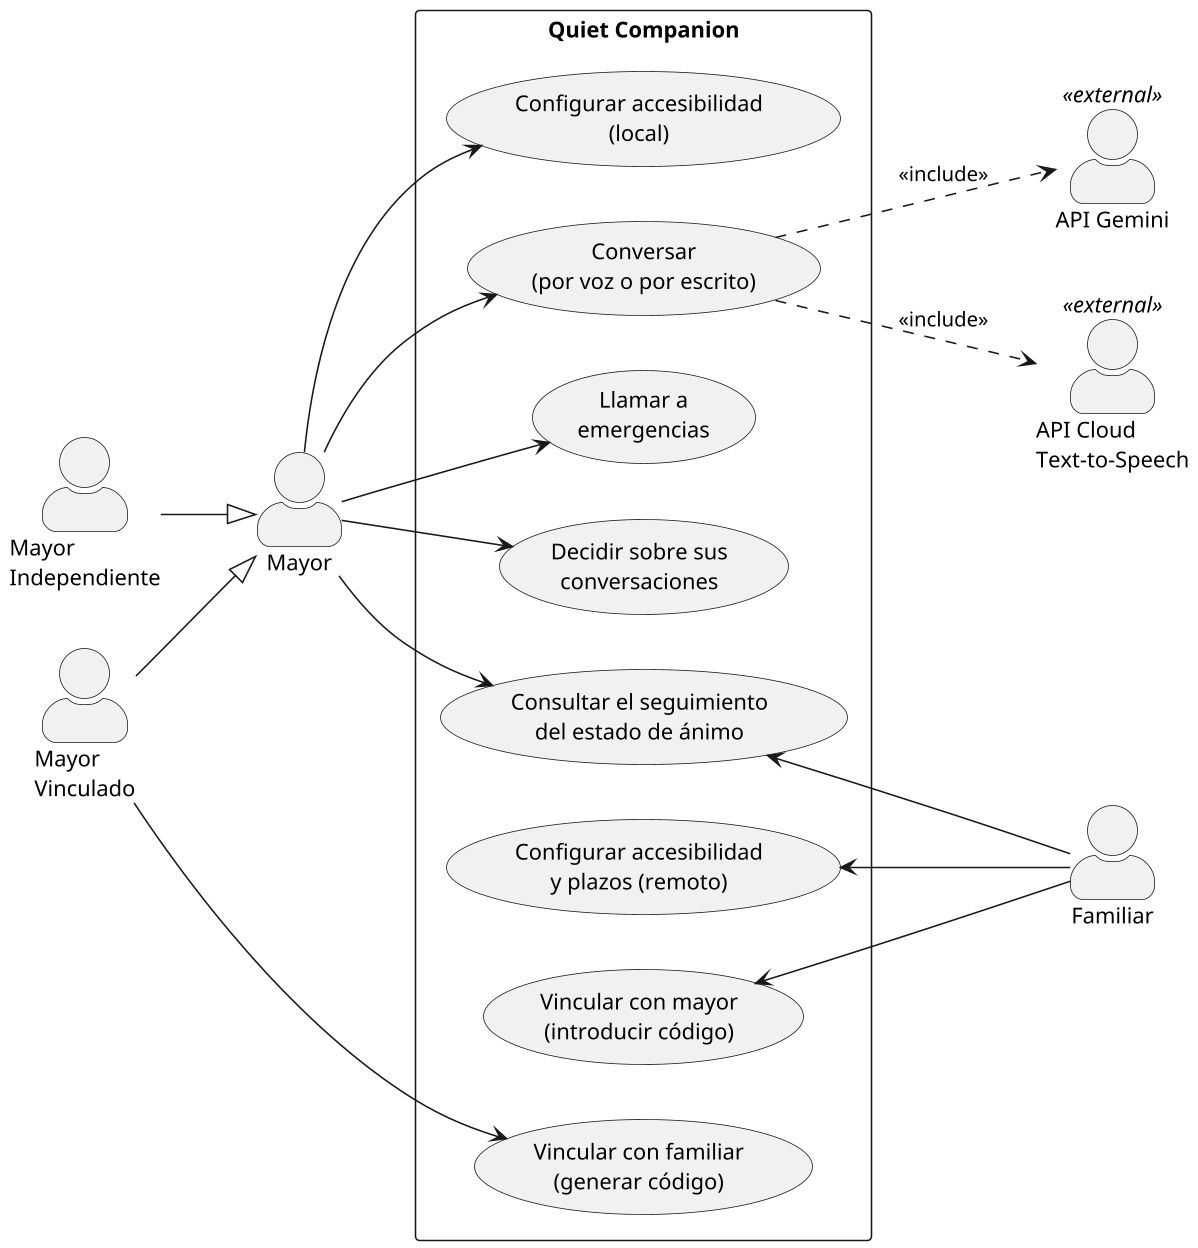
\includegraphics[width=0.8\textwidth]{imagenes/uml/diagrama_actores.png}
    \caption{Diagrama de actores del sistema.}
    \label{fig:actores}
\end{figure}

El diagrama agrupa los casos de uso por objetivo; su especificación, uno a uno, está en el apartado~\ref{sec:casos-de-uso}.

\section{Catálogo de requisitos}
Los requisitos se derivan de las ocho Historias de Usuario y de los tres principios de diseño del capítulo~\ref{cap:introduccion}. Los \textbf{requisitos funcionales} (RF) describen lo que hace el sistema, y los \textbf{no funcionales} (RNF), las condiciones en que debe hacerlo.

\subsection{Historias de Usuario}

La tabla~\ref{tab:enunciado-hu} recoge el enunciado de las ocho Historias de Usuario con el formato habitual de rol, necesidad y beneficio. La tarjeta completa de HU-1, con su estimación y sus criterios de aceptación, aparece como ejemplo en el capítulo~\ref{cap:metodologia}; los criterios de las demás se concretan aquí en requisitos y casos de uso. HU-4 y HU-6 nombran dos roles porque sirven a los dos: la configuración puede ajustarla el mayor o su familiar, y el seguimiento del ánimo lo consultan ambos.


\begin{table}[htbp]
    \centering
    \caption{Enunciado de las Historias de Usuario.}
    \label{tab:enunciado-hu}
    \small
    \begin{tabularx}{\textwidth}{@{}c >{\RaggedRight\arraybackslash}X@{}}
        \toprule
        \textbf{ID} & \textbf{Enunciado} \\
        \midrule
        HU-1 & Como mayor, quiero elegir al abrir la aplicación por primera vez si la gestionaré yo mismo o si me ayudará un familiar, para que el sistema me ofrezca la experiencia adecuada a mis capacidades tecnológicas. \\
        \addlinespace
        HU-2 & Como mayor, quiero conversar con el asistente pulsando un único botón y hablando con naturalidad, para tener compañía sin necesidad de aprender a usar la aplicación. \\
        \addlinespace
        HU-3 & Como mayor con la vista o la destreza mermadas, quiero textos grandes, botones amplios y una única forma de tocar la pantalla, para usar la aplicación sin ayuda. \\
        \addlinespace
        HU-4 & Como familiar, quiero ajustar desde mi móvil la voz del asistente, el volumen, la velocidad de la voz y el tamaño del texto del mayor, y que los cambios le lleguen al momento, para adaptarle la aplicación sin estar a su lado; y como mayor, quiero poder ajustarlos yo mismo. \\
        \addlinespace
        HU-5 & Como mayor, quiero que el asistente recuerde lo que le he contado en conversaciones anteriores, para no tener que repetirlo y sentir que me conoce. \\
        \addlinespace
        HU-6 & Como familiar, quiero saber cómo se ha encontrado el mayor durante la semana, para acompañarle mejor; y como mayor, quiero ver ese mismo resumen, para darme cuenta de cómo me siento y de lo que me preocupa. \\
        \addlinespace
        HU-7 & Como mayor, quiero decidir si se guardan mis conversaciones y qué parte ve mi familiar, y poder cambiarlo cuando quiera, para que nadie sepa de mí más de lo que yo autorice. \\
        \addlinespace
        HU-8 & Como mayor, quiero poder escribir en lugar de hablar cuando no pueda o no quiera usar la voz, para seguir conversando en silencio o cuando el reconocimiento de voz me falle. \\
        \bottomrule
    \end{tabularx}

\end{table}

\subsection{Requisitos funcionales}
Los requisitos funcionales se formalizan según una plantilla común: identificador, nombre, descripción, entradas, salidas, prioridad e Historia de Usuario asociada.

\begin{table}[htbp]
    \centering
    \caption{Requisito Funcional RF-1: Acceso y Selección Inicial de Modo de Uso.}
    \label{tab:rf1}
    \renewcommand{\arraystretch}{1.3}
    \begin{tabular}{|l|>{\raggedright\arraybackslash}p{0.72\textwidth}|}
        \hline
        \multicolumn{2}{|c|}{\textbf{Requisito Funcional: Acceso y Selección Inicial de Modo de Uso}} \\
        \hline
        \textbf{ID} & RF-1 \\
        \hline
        \textbf{Origen} & HU-1 \\
        \hline
        \textbf{Prioridad} & Alta \\
        \hline
        \textbf{Descripción} & Sin sesión iniciada, el sistema debe permitir al mayor entrar con su cuenta de Google o sin registrarse y presentarle después dos opciones excluyentes, usar la aplicación por su cuenta o vincularla con un familiar, y configurar el perfil según la elección. Si la cuenta de Google ya tiene un perfil, debe recuperarlo. \\
        \hline
        \textbf{Entradas} & Forma de acceso y modo elegidos en la pantalla de \textit{onboarding}. \\
        \hline
        \textbf{Salidas} & Perfil de usuario creado en la base de datos con \code{role = elder} y \code{autonomy} $\in$ \{\code{independent}, \code{dependent}\}, o el perfil ya existente de esa cuenta. \\
        \hline
    \end{tabular}

\end{table}

\begin{table}[htbp]
    \centering
    \caption{Requisito Funcional RF-2: Generación y Consumo de Código de Vinculación.}
    \label{tab:rf2}
    \renewcommand{\arraystretch}{1.3}
    \begin{tabular}{|l|>{\raggedright\arraybackslash}p{0.72\textwidth}|}
        \hline
        \multicolumn{2}{|c|}{\textbf{Requisito Funcional: Generación y Consumo de Código de Vinculación}} \\
        \hline
        \textbf{ID} & RF-2 \\
        \hline
        \textbf{Origen} & HU-1 \\
        \hline
        \textbf{Prioridad} & Alta \\
        \hline
        \textbf{Descripción} & Si el mayor opta por el modo vinculado, el sistema debe generar un código corto de 4~caracteres en su dispositivo. El familiar, desde su propio dispositivo, debe poder introducir dicho código para completar el emparejamiento de forma atómica, sin que pueda quedar un estado intermedio en el que solo uno de los dos perfiles esté vinculado. \\
        \hline
        \textbf{Entradas} & Solicitud de generación de código (mayor) e introducción del código (familiar). \\
        \hline
        \textbf{Salidas} & Vinculación bidireccional persistida en la base de datos: el campo \code{linkedCompanionId} en el perfil del mayor y \code{linkedElderId} en el del familiar, ambos escritos dentro de una misma transacción. \\
        \hline
    \end{tabular}

\end{table}

\begin{table}[htbp]
    \centering
    \caption{Requisito Funcional RF-3: Procesamiento Conversacional por Voz.}
    \label{tab:rf3}
    \renewcommand{\arraystretch}{1.3}
    \begin{tabular}{|l|>{\raggedright\arraybackslash}p{0.72\textwidth}|}
        \hline
        \multicolumn{2}{|c|}{\textbf{Requisito Funcional: Procesamiento Conversacional por Voz}} \\
        \hline
        \textbf{ID} & RF-3 \\
        \hline
        \textbf{Origen} & HU-2 \\
        \hline
        \textbf{Prioridad} & Alta \\
        \hline
        \textbf{Descripción} & El sistema debe permitir al mayor mantener una conversación por voz pulsando un único botón central. La entrada de voz se transcribe a texto, se envía al modelo de lenguaje y la respuesta se reproduce mediante síntesis de voz. \\
        \hline
        \textbf{Entradas} & Pulsación del botón principal; señal de audio del usuario. \\
        \hline
        \textbf{Salidas} & Respuesta del asistente reproducida por audio y mostrada en pantalla con tipografía de gran tamaño. \\
        \hline
    \end{tabular}

\end{table}

\begin{table}[htbp]
    \centering
    \caption{Requisito Funcional RF-4: Indicación Visual del Estado del Asistente.}
    \label{tab:rf4}
    \renewcommand{\arraystretch}{1.3}
    \begin{tabular}{|l|>{\raggedright\arraybackslash}p{0.72\textwidth}|}
        \hline
        \multicolumn{2}{|c|}{\textbf{Requisito Funcional: Indicación Visual del Estado del Asistente}} \\
        \hline
        \textbf{ID} & RF-4 \\
        \hline
        \textbf{Origen} & HU-2, HU-3 \\
        \hline
        \textbf{Prioridad} & Alta \\
        \hline
        \textbf{Descripción} & Durante una interacción de voz, el sistema debe comunicar visualmente en qué estado se encuentra, mediante las etiquetas <<Te escucho>>, <<Pensando>> y <<Respondiendo>>. La señalización debe ser perceptible por usuarios con limitaciones visuales moderadas y no puede descansar únicamente en el color. \\
        \hline
        \textbf{Entradas} & Cambios de estado internos del pipeline conversacional. \\
        \hline
        \textbf{Salidas} & Indicador visual y textual en pantalla. \\
        \hline
    \end{tabular}

\end{table}

\begin{table}[htbp]
    \centering
    \caption{Requisito Funcional RF-5: Configuración de Parámetros de Accesibilidad.}
    \label{tab:rf5}
    \renewcommand{\arraystretch}{1.3}
    \begin{tabular}{|l|>{\raggedright\arraybackslash}p{0.72\textwidth}|}
        \hline
        \multicolumn{2}{|c|}{\textbf{Requisito Funcional: Configuración de Parámetros de Accesibilidad}} \\
        \hline
        \textbf{ID} & RF-5 \\
        \hline
        \textbf{Origen} & HU-4 \\
        \hline
        \textbf{Prioridad} & Alta \\
        \hline
        \textbf{Descripción} & El sistema debe permitir configurar la voz del asistente, su volumen y su velocidad, el tamaño del texto y el tiempo de silencio tras el que el asistente da por terminado el turno del mayor. Todo mayor, independiente o vinculado, debe poder ajustarlos desde su propio dispositivo; si está vinculado, su familiar puede cambiar también desde el panel la voz, el volumen, la velocidad y el tamaño del texto. \\
        \hline
        \textbf{Entradas} & Valores de los parámetros configurables. \\
        \hline
        \textbf{Salidas} & Preferencias persistidas en la base de datos y aplicadas en la siguiente interacción del mayor. \\
        \hline
    \end{tabular}

\end{table}

\begin{table}[htbp]
    \centering
    \caption{Requisito Funcional RF-6: Propagación Remota de la Configuración.}
    \label{tab:rf6}
    \renewcommand{\arraystretch}{1.3}
    \begin{tabular}{|l|>{\raggedright\arraybackslash}p{0.72\textwidth}|}
        \hline
        \multicolumn{2}{|c|}{\textbf{Requisito Funcional: Propagación Remota de la Configuración}} \\
        \hline
        \textbf{ID} & RF-6 \\
        \hline
        \textbf{Origen} & HU-4 \\
        \hline
        \textbf{Prioridad} & Alta \\
        \hline
        \textbf{Descripción} & Cuando el familiar modifica las preferencias del mayor desde su panel remoto, los cambios deben propagarse en tiempo real al dispositivo del mayor, sin reiniciar la aplicación y sin que el mayor intervenga. \\
        \hline
        \textbf{Entradas} & Modificación de preferencias en el panel del familiar. \\
        \hline
        \textbf{Salidas} & Actualización efectiva de los parámetros en el dispositivo del mayor. \\
        \hline
    \end{tabular}

\end{table}

\begin{table}[htbp]
    \centering
    \caption{Requisito Funcional RF-7: Memoria Conversacional Contextualizada.}
    \label{tab:rf7}
    \renewcommand{\arraystretch}{1.3}
    \begin{tabular}{|l|>{\raggedright\arraybackslash}p{0.72\textwidth}|}
        \hline
        \multicolumn{2}{|c|}{\textbf{Requisito Funcional: Memoria Conversacional Contextualizada}} \\
        \hline
        \textbf{ID} & RF-7 \\
        \hline
        \textbf{Origen} & HU-5 \\
        \hline
        \textbf{Prioridad} & Media \\
        \hline
        \textbf{Descripción} & Al cerrar cada conversación, el sistema debe extraer de ella los datos estables del mayor (las personas de su entorno y su relación con ellas, dónde vive, sus aficiones o sus rutinas, excepto cualquier dato de salud) junto a un resumen breve, guardarlos en un documento de memoria aparte del registro de conversaciones, e incluir ese documento en el contexto del modelo al empezar la conversación siguiente, para que el asistente tenga en cuenta lo hablado antes. El nombre del mayor, que hace falta en la misma conversación, se aprende en cuanto lo dice. \\
        \hline
        \textbf{Entradas} & Transcripción de la conversación que se cierra y documento de memoria vigente del mayor. \\
        \hline
        \textbf{Salidas} & Documento de memoria actualizado y respuestas del asistente que reflejan el contexto personalizado del usuario. \\
        \hline
    \end{tabular}

\end{table}

\begin{table}[htbp]
    \centering
    \caption{Requisito Funcional RF-8: Catalogación Emocional de las Conversaciones.}
    \label{tab:rf8}
    \renewcommand{\arraystretch}{1.3}
    \begin{tabular}{|l|>{\raggedright\arraybackslash}p{0.72\textwidth}|}
        \hline
        \multicolumn{2}{|c|}{\textbf{Requisito Funcional: Catalogación Emocional de las Conversaciones}} \\
        \hline
        \textbf{ID} & RF-8 \\
        \hline
        \textbf{Origen} & HU-6 \\
        \hline
        \textbf{Prioridad} & Media \\
        \hline
        \textbf{Descripción} & Al terminar una conversación, el sistema debe clasificar el sentimiento general que expresa el mayor (Positivo, Neutro o Negativo), detectar las señales de una lista cerrada que él mismo manifieste (soledad, tristeza, preocupación, malestar físico, desorientación y riesgo), identificar los temas tratados y generar un resumen, todo ello en el servidor y sin almacenar la transcripción. La agregación semanal debe mostrarse al propio mayor (<<Mi semana>>) y, en lo que él autorice, en el panel del familiar. \\
        \hline
        \textbf{Entradas} & Transcripción de la conversación finalizada, retenida únicamente en memoria durante el análisis. \\
        \hline
        \textbf{Salidas} & Sentimiento, señales, temas y resumen almacenados en el registro de la conversación, y agregado semanal visible en la vista del mayor y en el panel de bienestar del familiar. \\
        \hline
    \end{tabular}

\end{table}

\begin{table}[htbp]
    \centering
    \caption{Requisito Funcional RF-9: Consentimiento y Control del Tratamiento Conversacional.}
    \label{tab:rf9}
    \renewcommand{\arraystretch}{1.3}
    \begin{tabular}{|l|>{\raggedright\arraybackslash}p{0.72\textwidth}|}
        \hline
        \multicolumn{2}{|c|}{\textbf{Requisito Funcional: Consentimiento y Control del Tratamiento}} \\
        \hline
        \textbf{ID} & RF-9 \\
        \hline
        \textbf{Origen} & HU-7 (deriva de RNF-10) \\
        \hline
        \textbf{Prioridad} & Alta \\
        \hline
        \textbf{Descripción} & El tratamiento de las conversaciones debe depender de un consentimiento explícito del propio mayor, desactivado por omisión, revocable en cualquier momento con la misma facilidad con que se dio y que el familiar no puede otorgar en su nombre. El mayor debe poder decidir además qué parte del análisis ve su familiar, y esa decisión debe aplicarse en el servidor, no solo en la interfaz. Los plazos de cierre por inactividad y de conservación de los datos derivados deben ser configurables dentro de los márgenes que fije el servidor. \\
        \hline
        \textbf{Entradas} & Gesto explícito del mayor en la pantalla de consentimiento, y ajustes de compartición y de plazos. \\
        \hline
        \textbf{Salidas} & Estado de consentimiento, ámbito de compartición y plazos persistidos en el perfil, y reglas de seguridad que los aplican a toda lectura del familiar. \\
        \hline
    \end{tabular}

\end{table}

\begin{table}[htbp]
    \centering
    \caption{Requisito Funcional RF-10: Conversación por Escrito.}
    \label{tab:rf10}
    \renewcommand{\arraystretch}{1.3}
    \begin{tabular}{|l|>{\raggedright\arraybackslash}p{0.72\textwidth}|}
        \hline
        \multicolumn{2}{|c|}{\textbf{Requisito Funcional: Conversación por Escrito}} \\
        \hline
        \textbf{ID} & RF-10 \\
        \hline
        \textbf{Origen} & HU-8 \\
        \hline
        \textbf{Prioridad} & Baja \\
        \hline
        \textbf{Descripción} & El sistema debe permitir al mayor alternar entre la voz y la escritura con un único botón de la pantalla principal. Un turno escrito debe seguir el mismo camino que uno hablado, también a efectos del análisis al cierre de la conversación, y su respuesta debe mostrarse en pantalla sin leerse en voz alta, salvo que el mayor lo pida. \\
        \hline
        \textbf{Entradas} & Texto introducido en el campo de escritura y pulsación de <<Enviar>>. \\
        \hline
        \textbf{Salidas} & Respuesta del asistente en pantalla con tipografía de gran tamaño, y su locución cuando el mayor pulsa <<Escuchar>>. \\
        \hline
    \end{tabular}

\end{table}

\begin{table}[htbp]
    \centering
    \caption{Requisito Funcional RF-11: Llamada de Emergencia.}
    \label{tab:rf11}
    \renewcommand{\arraystretch}{1.3}
    \begin{tabular}{|l|>{\raggedright\arraybackslash}p{0.72\textwidth}|}
        \hline
        \multicolumn{2}{|c|}{\textbf{Requisito Funcional: Llamada de Emergencia}} \\
        \hline
        \textbf{ID} & RF-11 \\
        \hline
        \textbf{Origen} & Seguridad del mayor (sin Historia de Usuario propia) \\
        \hline
        \textbf{Prioridad} & Media \\
        \hline
        \textbf{Descripción} & El sistema debe permitir al mayor llamar al 112 o a su contacto de emergencia desde la pantalla principal, sin que una pulsación accidental pueda iniciar la llamada. Si el mayor no ha fijado un contacto propio, la vinculación pone como tal a su familiar. \\
        \hline
        \textbf{Entradas} & Pulsación del botón de emergencia y elección del destino. \\
        \hline
        \textbf{Salidas} & Marcador del teléfono abierto con el número escrito. \\
        \hline
    \end{tabular}

\end{table}


\subsection{Requisitos no funcionales (RNF)}

Los requisitos no funcionales se agrupan en seis categorías y se aplican a todo el sistema salvo que se indique lo contrario.


\subsection*{Usabilidad y accesibilidad}
\begin{itemize}
    \item \textbf{RNF-1. Cumplimiento WCAG~2.2.} La interfaz dirigida al mayor debe cumplir los criterios de éxito de nivel~AA de la norma WCAG~2.2 \citep{wcag}, en particular los relativos a perceptibilidad (contraste, tamaño de texto) y operabilidad (área activa de elementos táctiles, ausencia de gestos complejos).
    \item \textbf{RNF-2. Áreas táctiles mínimas.} Todo elemento interactivo de la interfaz del mayor debe tener un área activa de al menos $80 \times 80$ píxeles lógicos.
    \item \textbf{RNF-3. Tipografías mínimas.} El texto de cuerpo en la interfaz del mayor debe presentarse a un tamaño mínimo de 20~sp y los títulos a un mínimo de 28~sp, sujetos al multiplicador definido por el usuario en sus preferencias.
    \item \textbf{RNF-4. Interacciones simples.} La interfaz del mayor debe operarse exclusivamente mediante pulsación simple, excluyéndose el doble toque, la pulsación prolongada y los gestos de deslizamiento.
    \item \textbf{RNF-5. Idioma.} Todos los textos de la interfaz, así como las entradas y salidas de voz, deben presentarse en español de España (es-ES).
\end{itemize}

\subsection*{Rendimiento}
\begin{itemize}
    \item \textbf{RNF-6. Plataforma objetivo.} El sistema debe ejecutarse correctamente en dispositivos Android con \code{minSdk = 24} (Android~7.0), que cubre los terminales de gama media y baja de 2016 en adelante.
    \item \textbf{RNF-7. Latencia de respuesta conversacional.} La latencia percibida entre el fin de la entrada de voz del usuario y el inicio de la respuesta sintetizada no debería superar los 3~segundos en condiciones normales de red y tras superar el \textit{cold start} en caso de haberlo.
\end{itemize}

\subsection*{Seguridad}
\begin{itemize}
    \item \textbf{RNF-8. Protección de credenciales de servicios externos.} Las claves de API de los servicios externos, en particular la de Gemini, no deben residir en el binario que se distribuye al usuario.
    \item \textbf{RNF-9. Aislamiento de identidades.} Las escrituras que afectan a documentos de un usuario distinto del autenticado, en particular el emparejamiento entre el mayor y el familiar, deben ejecutarse en un entorno servidor de confianza y no en el cliente.
\end{itemize}

\subsection*{Privacidad y protección de datos}
\begin{itemize}
    \item \textbf{RNF-10. Tratamiento de datos personales.} El sistema trata datos personales: identificadores de cuenta y, cuando los hay, el correo del familiar o el de la cuenta de Google del mayor, que conserva Firebase Authentication y no la base de datos; el nombre del mayor y los teléfonos de contacto; preferencias, resúmenes de las conversaciones, su categorización emocional y lo que el asistente recuerda del mayor. El tratamiento se ajusta al Reglamento General de Protección de Datos \citep{RGPD2016} y aplica los principios de minimización, limitación de la finalidad y limitación del plazo de conservación. En concreto, requiere el consentimiento explícito del mayor (RF-9); la transcripción no se almacena nunca y solo se procesa, de forma transitoria, para obtener el análisis y la memoria; las conversaciones en las que el mayor interviene menos de tres veces no se analizan, y de ellas solo sale del dispositivo la constancia de que existieron; y los datos derivados se borran al cumplirse un plazo configurable, de noventa días por omisión y nunca superior a ciento ochenta.
\end{itemize}

\subsection*{Mantenibilidad}
\begin{itemize}
    \item \textbf{RNF-11. Arquitectura.} El código fuente debe organizarse según el modelo Clean Architecture combinado con Feature-Sliced Design (CFS), con separación estricta entre las capas de presentación, dominio y datos, y sin acoplamiento horizontal entre \textit{features}.
    \item \textbf{RNF-12. Inyección de dependencias.} Los servicios externos y repositorios deben inyectarse en los controladores mediante los proveedores de Riverpod (apartado~\ref{sec:estado-di}), evitando instanciación directa dentro de la lógica de negocio.
    \item \textbf{RNF-13. Calidad estática.} Todo módulo modificado debe superar el análisis estático (\code{flutter analyze}) sin advertencias antes de su integración en la rama principal.
\end{itemize}

\subsection*{Disponibilidad}
\begin{itemize}
    \item \textbf{RNF-14. Dependencia de conectividad.} El sistema necesita conexión a internet para conversar (API de Gemini) y para sincronizar (Firestore). Si la conexión falla, debe avisar al usuario en lugar de fallar en silencio.
\end{itemize}

\section{Casos de uso}
\label{sec:casos-de-uso}
Esta sección especifica los casos de uso del sistema. Los seis primeros corresponden a HU-1 a HU-4, el núcleo de la aplicación, y los cuatro siguientes a HU-5 a HU-8, que se apoyan en él: CU-07 recoge el consentimiento del mayor, CU-08 y CU-09 lo exigen como precondición, y CU-10 añade a la conversación de CU-04 un segundo canal de entrada. CU-11, la llamada de emergencia, no procede de ninguna historia, sino de la seguridad del mayor (RF-11).

\subsection{Diagramas de casos de uso (UML)}

El diagrama de la \autoref{fig:casos-de-uso} agrupa a los dos perfiles de mayor bajo un actor común, del que ambos heredan, para no repetir las asociaciones que comparten; solo la generación del código de vinculación es exclusiva del mayor vinculado. CU-08 se asocia al mayor de forma implícita, porque no lo inicia un gesto suyo sino el final de la conversación.

\subsection{Especificación detallada}

Cada caso de uso se documenta según la plantilla habitual en ingeniería de requisitos \citep{Sommerville2016}: identificador, nombre, actor primario, precondiciones, flujo principal, flujos alternativos y postcondiciones.

\subsection*{CU-01. Seleccionar modo de uso}

\begin{figure}[p]
    \centering
    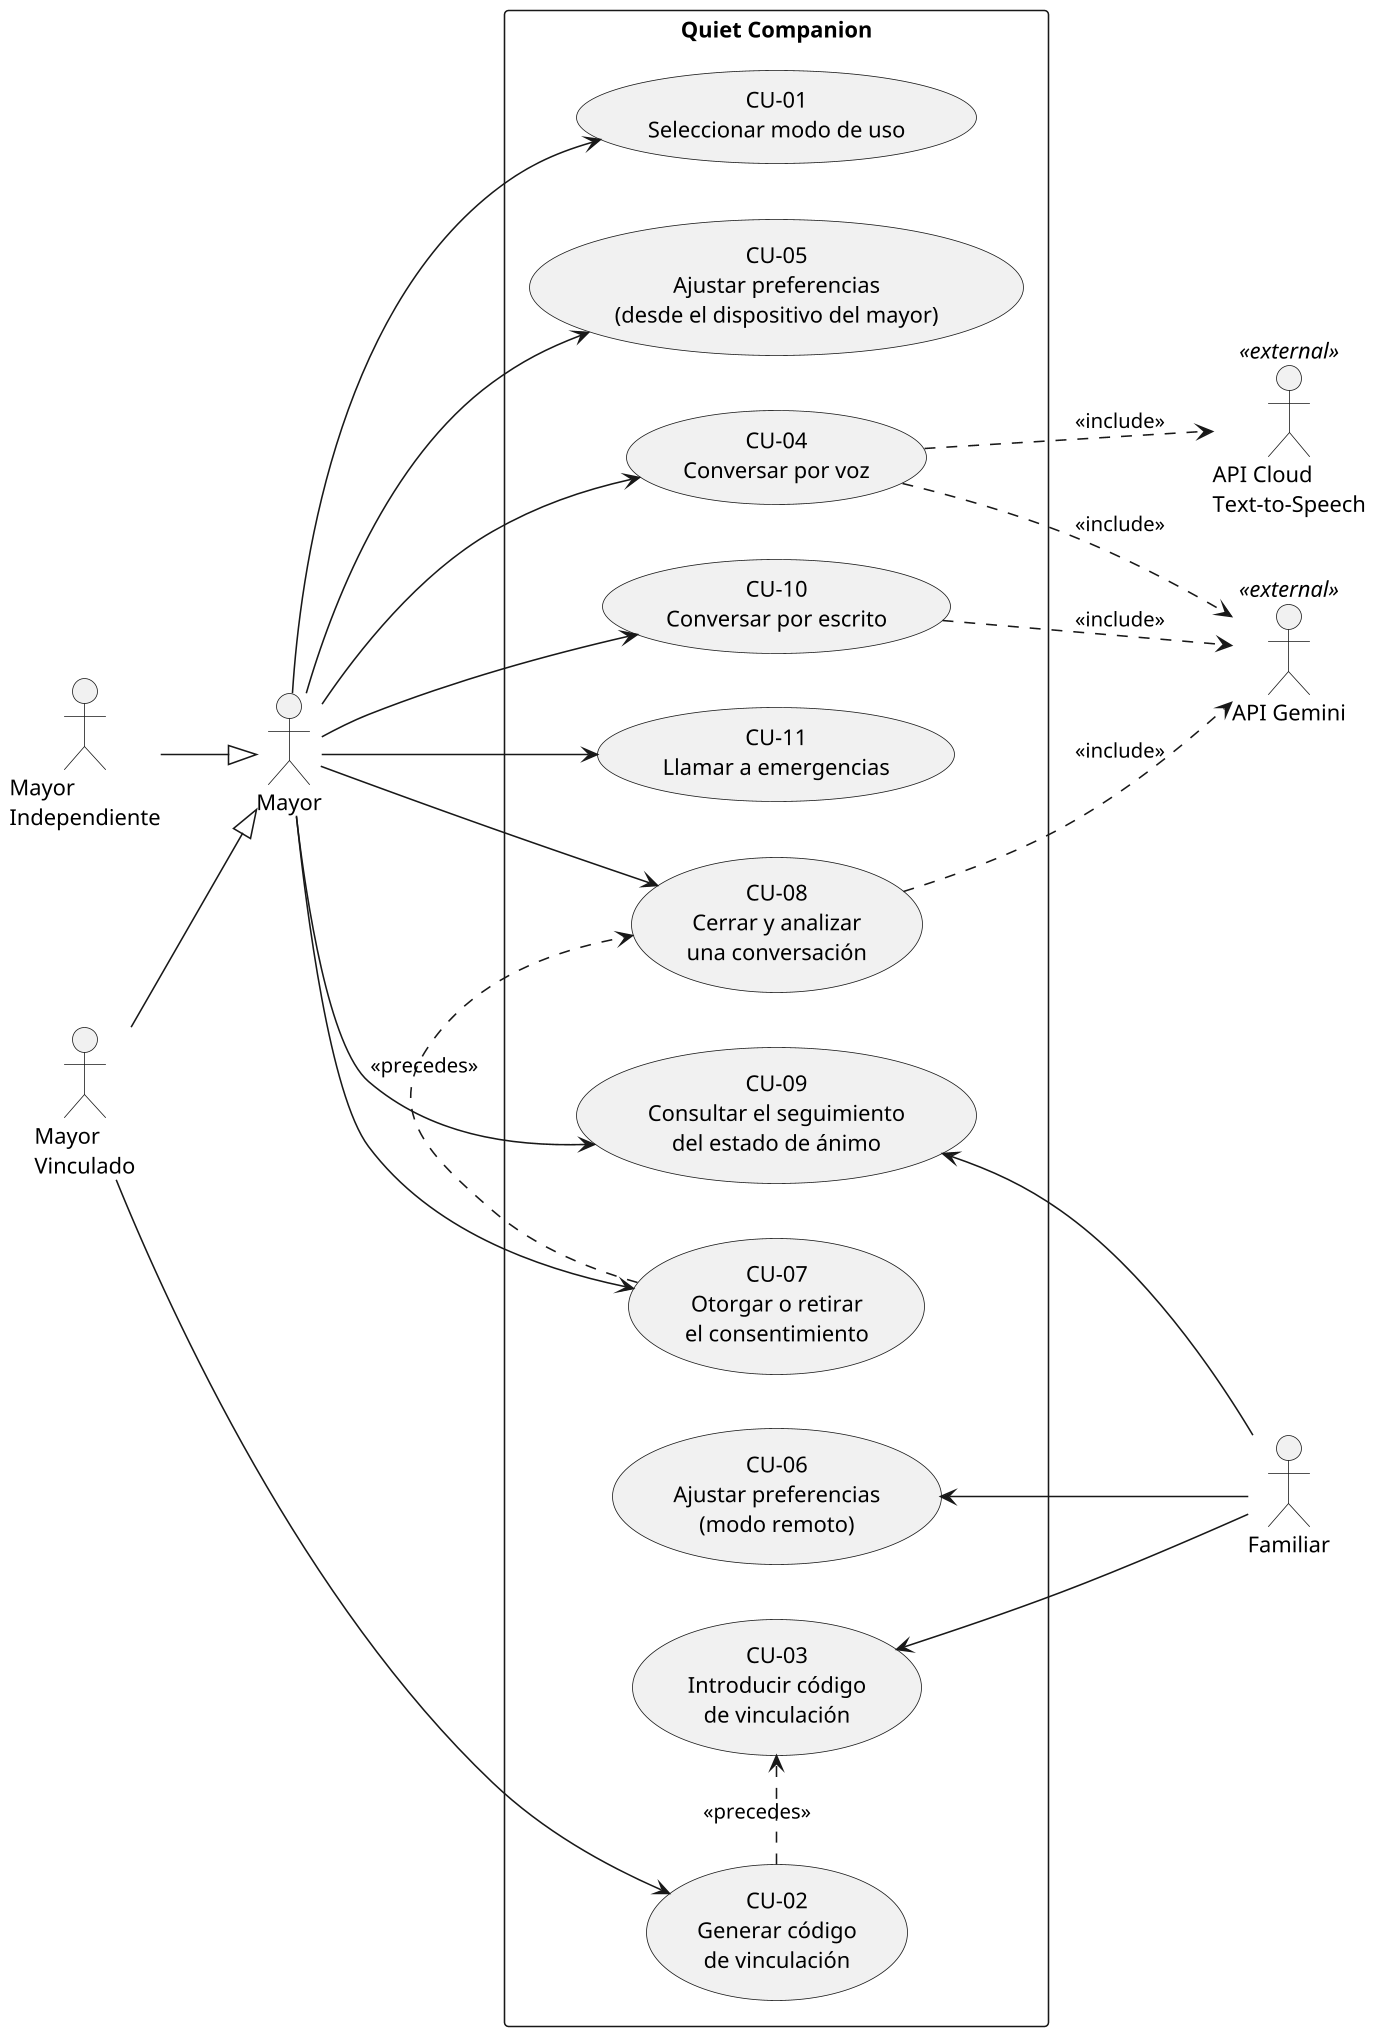
\includegraphics[width=\textwidth, height=0.9\textheight, keepaspectratio]{imagenes/uml/diagrama_casos_de_uso.png}
    \caption{Diagrama de casos de uso del sistema (CU-01 a CU-11).}
    \label{fig:casos-de-uso}
\end{figure}

\noindent\textbf{Actor primario:} Mayor (Independiente o Vinculado, según resultado del caso).

\noindent\textbf{Precondiciones:} No hay sesión iniciada: es el primer arranque de la aplicación en el dispositivo, el primero tras reinstalarla o el siguiente a cerrar la sesión.

\noindent\textbf{Flujo principal:}
\begin{enumerate}[nosep]
    \item El sistema pregunta cómo entrar, con dos botones de gran tamaño: \textit{<<Entrar con Google>>} y \textit{<<Entrar sin registrarme>>}.
    \item El usuario elige una de las dos vías; con Google, elige además su cuenta en el selector del teléfono.
    \item El sistema presenta dos botones de gran tamaño: \textit{<<Usar por mi cuenta>>} y \textit{<<\hspace{0pt}Vincular con mi familiar>>}.
    \item El usuario pulsa una de las dos opciones.
    \item El sistema crea el perfil en la base de datos con \code{role = elder}.
    \item Si la opción seleccionada es la primera, el sistema asigna \code{autonomy = independent} y presenta la pregunta del consentimiento (CU-07) antes de la pantalla principal.
    \item Si la opción seleccionada es la segunda, el sistema asigna \code{autonomy = dependent} y desencadena el caso de uso CU-02.
\end{enumerate}

\noindent\textbf{Flujos alternativos:}
\begin{itemize}[nosep]
    \item \textbf{2a.} La cuenta de Google ya tiene un perfil de mayor, por ejemplo el de un teléfono anterior: el sistema lo recupera tal cual y lleva al mayor a su pantalla principal.
    \item \textbf{2b.} La cuenta de Google es la de un familiar: el sistema cierra la sesión, lo avisa y vuelve al paso~1.
\end{itemize}

\noindent\textbf{Postcondiciones:} Existe un perfil de mayor en la base de datos con su \code{autonomy} definida.

\bigskip

\subsection*{CU-02. Generar código de vinculación}

\noindent\textbf{Actor primario:} Mayor Vinculado.

\noindent\textbf{Precondiciones:} Se ha completado CU-01 con \code{autonomy = dependent}.

\noindent\textbf{Flujo principal:}
\begin{enumerate}[nosep]
    \item El sistema genera un código aleatorio de 4~caracteres (alfanumérico, excluidos los caracteres confundibles O, 0, I y~1).
    \item El sistema persiste el código en el perfil del mayor y lo presenta en pantalla con tipografía de gran tamaño.
    \item El mayor permanece en esa pantalla, sin acceso todavía a la conversación, hasta que el familiar introduce el código (CU-03); entonces la pantalla avanza sola.
\end{enumerate}

\noindent\textbf{Flujos alternativos:}
\begin{itemize}[nosep]
    \item \textbf{3a.} El mayor pulsa <<Cancelar>>: el código se borra de su perfil y vuelve a la elección de modo (CU-01).
\end{itemize}

\noindent\textbf{Postcondiciones:} Existe un código de vinculación activo en el perfil del mayor, pendiente de ser consumido por un familiar.

\bigskip

\subsection*{CU-03. Introducir código de vinculación}

\noindent\textbf{Actor primario:} Familiar.

\noindent\textbf{Precondiciones:} El familiar tiene una cuenta autenticada (correo + contraseña) y posee un código de vinculación válido proporcionado por el mayor.

\noindent\textbf{Flujo principal:}
\begin{enumerate}[nosep]
    \item El familiar accede a la pantalla de emparejamiento desde su dispositivo.
    \item El familiar introduce el código de 4~caracteres.
    \item El sistema valida en el servidor que el código existe y no ha sido consumido, y comprueba que quien solicita la vinculación es un familiar registrado.
    \item El sistema ejecuta una operación atómica que actualiza, en una misma transacción, el campo \code{linkedCompanionId} del mayor y el campo \code{linkedElderId} del familiar, y consume el código para que no pueda reutilizarse.
    \item El sistema confirma la vinculación al familiar, y la aplicación del mayor deja la pantalla del código automáticamente.
\end{enumerate}

\noindent\textbf{Flujos alternativos:}
\begin{itemize}[nosep]
    \item \textbf{3a.} Código inexistente o ya consumido: el sistema muestra mensaje de error y permite     reintentar.
\end{itemize}

\noindent\textbf{Postcondiciones:} Mayor y familiar están vinculados en los dos sentidos y el código ha quedado consumido. El mayor pasa a la pregunta del consentimiento (CU-07) antes de la pantalla principal.

\bigskip

\subsection*{CU-04. Conversar por voz}

\noindent\textbf{Actor primario:} Mayor (cualquier modalidad).

\noindent\textbf{Actor secundario:} API de Gemini y API de Cloud Text-to-Speech.

\noindent\textbf{Precondiciones:} El mayor ha llegado a la pantalla principal (si es vinculado, tras completar CU-03) y el dispositivo tiene conexión a internet.

\noindent\textbf{Flujo principal:}
\begin{enumerate}[nosep]
    \item El mayor pulsa el botón central de micrófono en la pantalla principal.
    \item El sistema solicita permiso de micrófono si no estaba concedido, empieza a escuchar y muestra la etiqueta <<Te escucho>>.
    \item El sistema transcribe lo que dice el mayor con el reconocedor de voz (\code{es-ES}) y da el turno por terminado cuando guarda silencio durante el tiempo elegido en Ajustes.
    \item El sistema muestra <<Pensando>> y envía el texto a la API de Gemini, junto con la instrucción de sistema y lo que el asistente recuerda del mayor (RF-7).
    \item La API de Gemini devuelve una respuesta textual.
    \item El sistema muestra <<Respondiendo>> y la respuesta en pantalla con tipografía de gran tamaño, y se reproduce con la voz, el volumen y la velocidad elegidos. Si la síntesis en la nube falla o tarda, la respuesta se pronuncia con el motor de voz del propio dispositivo.
    \item Al terminar la reproducción, el sistema vuelve al estado de reposo.
\end{enumerate}

\noindent\textbf{Flujos alternativos:}
\begin{itemize}[nosep]
    \item \textbf{1a.} El mayor prefiere escribir: pulsa <<¿Teclado?>> y continúa en CU-10.
    \item \textbf{2a.} El micrófono no está disponible o se deniega el permiso: el sistema muestra <<No se ha podido acceder al micrófono>>, y el mayor puede seguir por escrito (CU-10).
    \item \textbf{4a.} Error de red o de la API: el sistema muestra <<Ups, ha habido un problema de conexión. ¿Puedes repetir?>>, y el micrófono queda listo para volver a intentarlo.
\end{itemize}

\noindent\textbf{Postcondiciones:} La interacción se ha completado o cancelado de forma controlada.

\bigskip

\subsection*{CU-05. Ajustar preferencias (desde el dispositivo del mayor)}

\noindent\textbf{Actor primario:} Mayor (Independiente o Vinculado).

\noindent\textbf{Precondiciones:} El mayor tiene un perfil activo y, si es vinculado, el emparejamiento se ha completado.

\noindent\textbf{Flujo principal:}
\begin{enumerate}[nosep]
    \item El mayor accede a la pantalla de ajustes desde la pantalla principal.
    \item El sistema muestra un menú de cuatro entradas a lo sumo. El mayor elige el tamaño de la letra, o abre el grupo <<Cómo hablamos>>, que reúne la voz, el volumen, la velocidad y el tiempo que el asistente le espera en silencio. Si es independiente, fija además en <<Mis conversaciones>> los plazos de sus conversaciones.
    \item El mayor modifica uno o varios parámetros. Las escalas se presentan como botones grandes (incremento / decremento) con peldaños con nombre, no como deslizadores; la voz, como una lista de cuatro opciones que suenan al tocarlas.
    \item Cada pulsación se persiste por sí sola en la base de datos, sin botón de guardar.
    \item Los nuevos parámetros se aplican inmediatamente a las próximas interacciones de voz y al renderizado de la interfaz.
\end{enumerate}

\noindent\textbf{Flujos alternativos:}
\begin{itemize}[nosep]
    \item \textbf{4a.} El mayor está vinculado y su familiar cambia el mismo parámetro desde el panel (CU-06): prevalece el último cambio, sin arbitraje, porque sobre la accesibilidad ninguno de los dos tiene una autoridad que proteger.
\end{itemize}

\noindent\textbf{Postcondiciones:} Las preferencias del mayor están actualizadas y aplicadas.

\bigskip

\subsection*{CU-06. Ajustar preferencias (modo remoto, desde el Familiar)}

\noindent\textbf{Actor primario:} Familiar.

\noindent\textbf{Precondiciones:} El familiar está vinculado a un mayor, es decir, existen \code{linkedElderId} en su perfil y \code{linkedCompanionId} en el del mayor.

\noindent\textbf{Flujo principal:}
\begin{enumerate}[nosep]
    \item El familiar accede al panel remoto desde su dispositivo.
    \item El sistema muestra el estado actual de las preferencias del mayor (la voz y tres deslizadores, para el volumen, la velocidad y el tamaño del texto) y los plazos de sus conversaciones.
    \item El familiar modifica uno o varios parámetros.
    \item Al soltar cada deslizador, o al elegir una voz o un plazo, el cambio se guarda en la base de datos.
    \item El cambio se propaga en tiempo real al dispositivo del mayor mediante la suscripción reactiva a su documento de usuario, sin que el mayor deba intervenir.
\end{enumerate}

\noindent\textbf{Flujos alternativos:}
\begin{itemize}[nosep]
    \item \textbf{4a.} Error al guardar: el control vuelve a su valor anterior y el panel avisa al familiar.
\end{itemize}

\noindent\textbf{Postcondiciones:} Las preferencias del mayor están actualizadas y aplicadas en su dispositivo.

\bigskip

\subsection*{CU-07. Otorgar o retirar el consentimiento sobre las conversaciones}

\noindent\textbf{Actor primario:} Mayor (Independiente o Vinculado).

\noindent\textbf{Precondiciones:} El mayor ha elegido el modo independiente (CU-01) o ha completado la vinculación (CU-03), y no ha respondido nunca a la pregunta. El consentimiento está desactivado por omisión.

\noindent\textbf{Flujo principal:}
\begin{enumerate}[nosep]
    \item Antes de llegar por primera vez a la pantalla principal, el sistema presenta una pantalla que explica en lenguaje llano qué se guarda, qué no y quién puede verlo: si está vinculado, su familiar, que verá cómo se encuentra y un resumen de lo que hablan; si no, solo él.
    \item El mayor responde <<Sí, quiero>> o <<Ahora no>>, con dos botones del mismo tamaño.
    \item La respuesta se registra mediante una función en la nube, único punto autorizado para escribir ese campo del perfil, junto con la hora del servidor y la versión del texto que el mayor ha leído.
\end{enumerate}

\noindent\textbf{Flujos alternativos:}
\begin{itemize}[nosep]
    \item \textbf{2a.} El mayor responde <<Ahora no>>: la aplicación conversa con normalidad, pero no se analiza ni se guarda nada de lo hablado, y no vuelve a preguntar.
    \item \textbf{3a.} El familiar intenta otorgar el consentimiento en nombre del mayor: el servidor rechaza la operación.
    \item \textbf{*a.} En cualquier momento, desde Ajustes, el mayor puede dar el consentimiento que negó, cambiar qué parte de su análisis ve su familiar o retirarlo. Si lo retira, el análisis se detiene, el familiar pierde al instante el acceso a lo guardado y eso se borra al cumplirse la mitad del plazo de conservación, salvo que el mayor vuelva a consentir antes.
\end{itemize}

\noindent\textbf{Postcondiciones:} El estado del consentimiento y el nivel de compartición quedan guardados y rigen toda lectura posterior.

\bigskip

\subsection*{CU-08. Cerrar y analizar una conversación}

\noindent\textbf{Actor primario:} Mayor, de forma implícita: lo dispara el final de la conversación, no un gesto suyo.

\noindent\textbf{Precondiciones:} Existe una conversación en curso y el mayor ha otorgado el consentimiento (CU-07).

\noindent\textbf{Flujo principal:}
\begin{enumerate}[nosep]
    \item El sistema detecta el final de la conversación: han pasado cinco minutos sin turnos (valor por omisión) o la aplicación ha pasado a segundo plano.
    \item Envía a una función en la nube la transcripción acumulada, que hasta ese momento solo ha existido en la memoria del teléfono.
    \item La función comprueba que el consentimiento sigue vigente y, con una sola llamada al modelo, obtiene el sentimiento, las señales, los temas, un resumen breve y los cambios en la memoria del mayor (RF-7).
    \item Guarda el registro de la conversación (actividad, ánimo y señales) y, en un documento aparte, su contenido (temas y resumen), y actualiza la memoria (\autoref{lst:modelo-datos}).
    \item Descarta la transcripción.
\end{enumerate}

\noindent\textbf{Flujos alternativos:}
\begin{itemize}[nosep]
    \item \textbf{1a.} El mayor sale al marcador de emergencia: la conversación no se cierra y continúa a su vuelta.
    \item \textbf{2a.} El mayor ha intervenido menos de tres veces: solo se envía la constancia de la conversación (inicio, fin y número de turnos), sin texto.
    \item \textbf{3a.} El modelo falla o no responde: la conversación se registra igualmente, con estado de fallo, y la memoria del mayor no se altera.
\end{itemize}

\noindent\textbf{Postcondiciones:} El registro de la conversación y la memoria del mayor quedan actualizados; la transcripción no se ha guardado en ningún soporte.

\bigskip

\subsection*{CU-09. Consultar el seguimiento del estado de ánimo}

\noindent\textbf{Actor primario:} Mayor, en su propia vista de resumen semanal (<<Mi semana>>), o Familiar, en el panel de bienestar.

\noindent\textbf{Precondiciones:} El mayor ha otorgado el consentimiento (CU-07) y existe al menos una conversación analizada. Para el familiar se exige además la vinculación activa.

\noindent\textbf{Flujo principal:}
\begin{enumerate}[nosep]
    \item El actor abre la vista que le corresponde según su rol.
    \item El sistema agrega los registros de conversación de los últimos siete días.
    \item Presenta los días en que hubo conversación, el ánimo predominante y los temas más repetidos; en el panel del familiar, además, las señales detectadas, los resúmenes y lo que el asistente recuerda, según lo que el mayor comparta.
    \item En la vista del mayor, la presentación sigue las restricciones de accesibilidad de HU-3: frases en lugar de gráficas, que además puede escuchar, y la indicación de qué parte de su análisis ve su familiar.
\end{enumerate}

\noindent\textbf{Flujos alternativos:}
\begin{itemize}[nosep]
    \item \textbf{2a.} No hay conversaciones analizadas en los últimos siete días: el sistema lo explica en lugar de mostrar una vista vacía que pudiera tomarse por un error.
    \item \textbf{3a.} El mayor ha restringido lo que comparte: el panel muestra solo lo autorizado y explica por qué falta el resto. La restricción la aplican las reglas de seguridad del servidor, no el cliente.
\end{itemize}

\noindent\textbf{Postcondiciones:} Ninguna. El caso es de solo lectura.

\bigskip

\subsection*{CU-10. Conversar por escrito}

\noindent\textbf{Actor primario:} Mayor (cualquier modalidad).

\noindent\textbf{Actor secundario:} API de Gemini.

\noindent\textbf{Precondiciones:} El mayor tiene un perfil activo y el dispositivo dispone de conexión a internet.

\noindent\textbf{Flujo principal:}
\begin{enumerate}[nosep]
    \item El mayor pulsa <<¿Teclado?>> en la pantalla principal.
    \item El sistema sustituye el botón del micrófono por un campo de texto y un botón <<Enviar>>, y abre el teclado del dispositivo sin necesidad de otro toque.
    \item El mayor escribe su mensaje y pulsa <<Enviar>>.
    \item El sistema cierra el teclado, muestra el estado <<Pensando>> y envía el texto al modelo de lenguaje como un turno más de la conversación en curso.
    \item El sistema muestra la respuesta en pantalla con tipografía de gran tamaño, sin leerla en voz alta.
    \item Si el mayor pulsa <<Escuchar>>, el sistema lee la respuesta, y el botón pasa a <<Parar>> mientras suena.
\end{enumerate}

\noindent\textbf{Flujos alternativos:}
\begin{itemize}[nosep]
    \item \textbf{1a.} El micrófono estaba escuchando: lo oído se descarta sin enviarse.
    \item \textbf{4a.} Error de red o de la API: el sistema muestra un mensaje accesible y devuelve el texto al campo, para no obligar a escribirlo de nuevo.
    \item \textbf{6a.} El mayor pulsa <<¿Hablar?>>: el sistema vuelve al modo de voz (CU-04).
\end{itemize}

\noindent\textbf{Postcondiciones:} El turno escrito forma parte de la conversación en curso y cuenta para su análisis al cierre (CU-08) exactamente igual que uno hablado.

\bigskip

\subsection*{CU-11. Llamar a emergencias}

\noindent\textbf{Actor primario:} Mayor (cualquier modalidad).

\noindent\textbf{Precondiciones:} El mayor ha llegado a la pantalla principal.

\noindent\textbf{Flujo principal:}
\begin{enumerate}[nosep]
    \item El mayor pulsa el botón rojo de emergencia de la pantalla principal.
    \item El sistema abre a pantalla completa la pantalla de emergencia, con <<Llamar al 112>> y, si hay contacto de emergencia, <<Llamar a>> seguido de su nombre.
    \item El mayor elige uno de los dos.
    \item El sistema abre el marcador del teléfono con el número escrito, y el mayor pulsa llamar.
\end{enumerate}

\noindent\textbf{Flujos alternativos:}
\begin{itemize}[nosep]
    \item \textbf{3a.} El mayor pulsa <<Cancelar>>: vuelve a la pantalla principal sin llamar.
    \item \textbf{4a.} El marcador no se puede abrir: el sistema lo avisa en la propia pantalla.
\end{itemize}

\noindent\textbf{Postcondiciones:} Si había una conversación en curso, sigue abierta al volver (CU-08).


\subsection{Trazabilidad}

La tabla~\ref{tab:trazabilidad} cruza Historias de Usuario, requisitos funcionales y casos de uso. Con ella se comprueba que cada requisito y cada caso de uso responde a una necesidad del usuario, y que cada historia, salvo HU-3, tiene al menos un caso de uso que la realiza.

\begin{table}[htbp]
    \centering
    \caption{Trazabilidad entre Historias de Usuario, Requisitos funcionales y Casos de uso.}
    \label{tab:trazabilidad}
    \begin{tabularx}{\textwidth}{@{}c >{\RaggedRight\arraybackslash}X >{\RaggedRight\arraybackslash}X@{}}
        \toprule
        \textbf{Historia de Usuario} & \textbf{Requisitos funcionales} & \textbf{Casos de uso} \\
        \midrule
        HU-1 & RF-1, RF-2                & CU-01, CU-02, CU-03 \\
        HU-2 & RF-3                      & CU-04 \\
        HU-3 & RF-4                      & No procede \\
        HU-4 & RF-5, RF-6                & CU-05, CU-06 \\
        HU-5 & RF-7                      & CU-08 \\
        HU-6 & RF-8                      & CU-08, CU-09 \\
        HU-7 & RF-9                      & CU-07 \\
        HU-8 & RF-10                     & CU-10 \\
        No procede & RF-11               & CU-11 \\
        \bottomrule
    \end{tabularx}

\end{table}

HU-3 no tiene casos de uso propios: sus criterios son restricciones de accesibilidad que afectan a todos los casos de uso del mayor y se recogen como RNF-1 a RNF-4. Su único requisito funcional, RF-4, se cumple dentro de CU-04 y CU-10.

RF-11 y CU-11, la llamada de emergencia, no tienen historia propia: responden a la seguridad del mayor, que ninguna historia formula y que la aplicación no puede dejar sin cubrir.

RF-9 y CU-07 se asignan a HU-7, y no a HU-5 o HU-6, porque el consentimiento responde a una necesidad propia del mayor: decidir qué se guarda de él y quién lo ve. HU-5 y HU-6 dependen de él a través de las precondiciones de CU-08 y CU-09, y RNF-10 recoge las garantías que lo rodean.

\section{Modelo conceptual de dominio}

El modelo conceptual de la \autoref{fig:dominio} recoge las entidades que maneja el sistema y sus relaciones, sin entrar en cómo se implementan.

\begin{figure}[tbp]
    \centering
    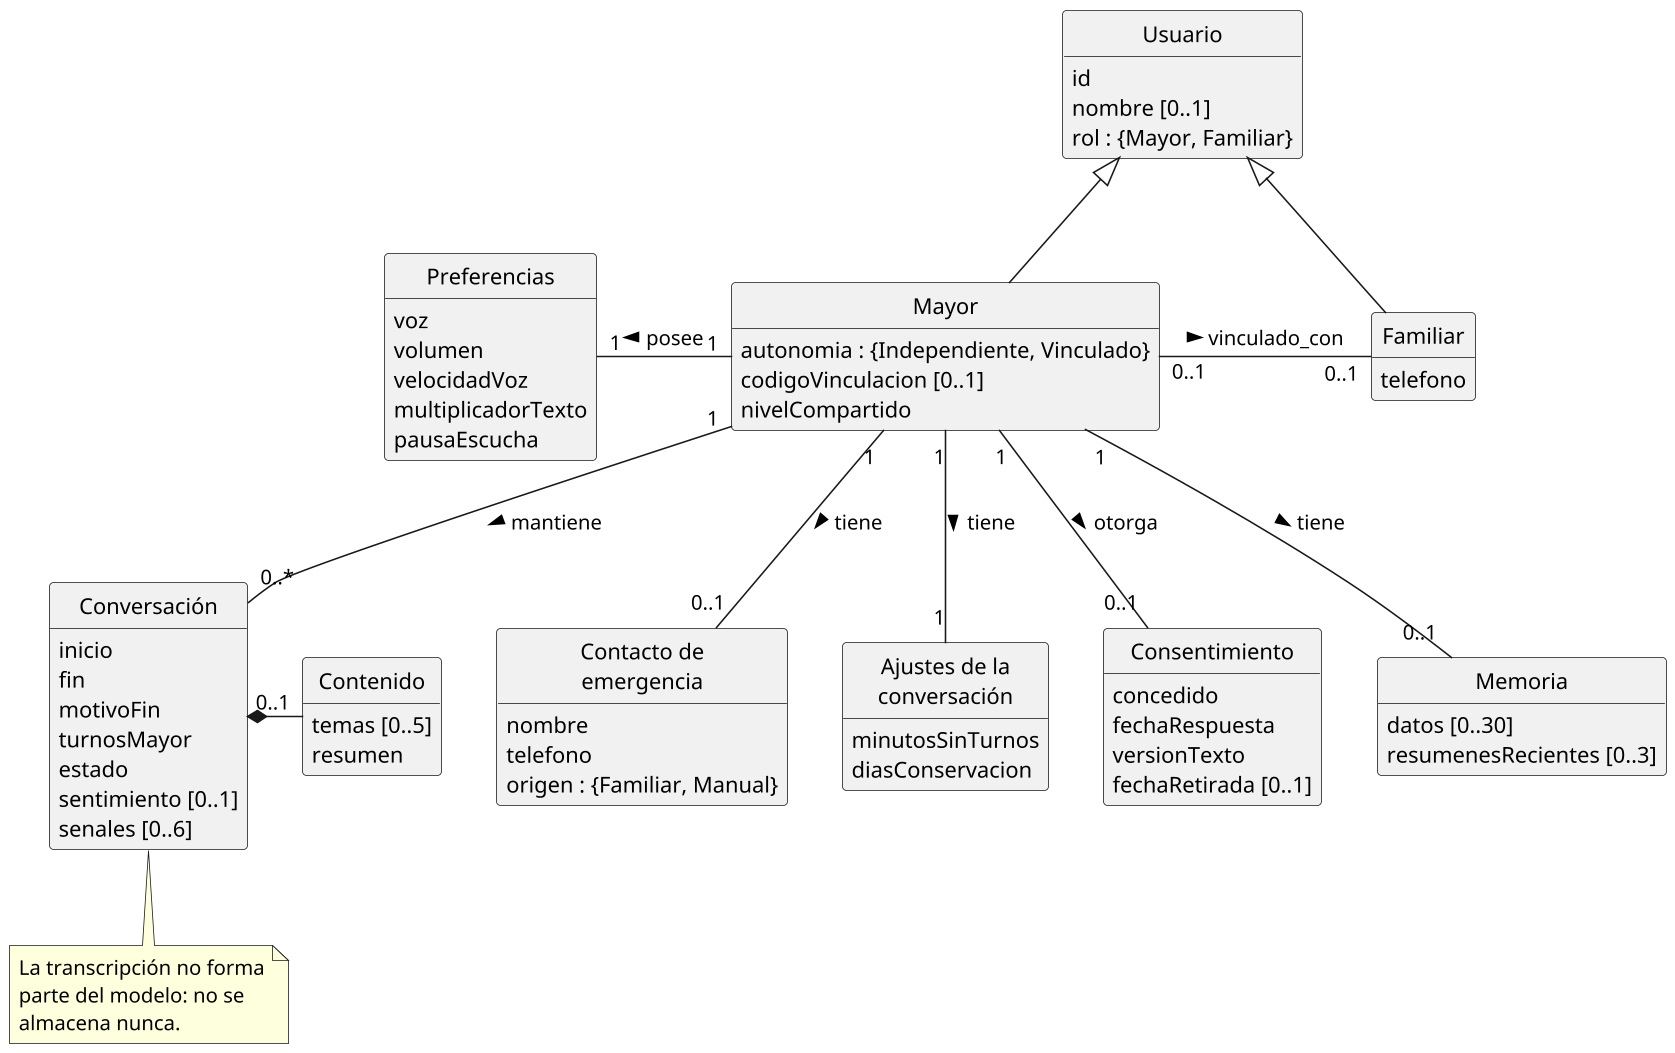
\includegraphics[width=\textwidth]{imagenes/uml/diagrama_conceptual.png}
    \caption{Modelo conceptual de dominio del sistema.}
    \label{fig:dominio}
\end{figure}

El sistema maneja ocho entidades. El \textbf{Usuario} es una persona que usa el sistema, con un rol, \textit{Mayor} o \textit{Familiar}. El mayor tiene además un grado de autonomía, que distingue al independiente del vinculado, y un nivel de compartición, que fija qué parte de su análisis ve el familiar, mientras que el familiar tiene un número de teléfono asociado. Las \textbf{Preferencias} son los ajustes de accesibilidad y de voz del mayor: la voz, su volumen y su velocidad, el multiplicador del tamaño de texto y el tiempo de silencio que cierra su turno. Los \textbf{Ajustes de la conversación} son los dos plazos que gobiernan sus datos: el tiempo sin turnos tras el que una conversación se da por terminada y el tiempo durante el que se conserva lo analizado. El \textbf{Consentimiento} es la respuesta del mayor a la pregunta de si se guardan sus conversaciones, con la fecha en que la dio, la versión del texto que leyó y, si lo retiró, la fecha de retirada. La \textbf{Conversación} es un intercambio entre el mayor y el asistente, delimitado por un periodo sin turnos o por la salida de la aplicación, con sus datos de actividad y el sentimiento y las señales detectados; su \textbf{Contenido}, los temas y el resumen, es una entidad aparte. La \textbf{Memoria} reúne lo que el asistente recuerda del mayor: un conjunto acotado de datos estables y los resúmenes de las últimas conversaciones. El \textbf{Contacto de emergencia}, por último, es la persona a la que el mayor puede llamar desde la pantalla de emergencia, con su nombre, su teléfono y su origen: el familiar, si lo fijó la vinculación, o el propio mayor, si lo introdujo a mano.

La transcripción no forma parte del modelo, pues existe mientras dura la conversación y mientras se analiza, pero no se guarda en ningún soporte. Lo que el sistema almacena es, por tanto, un subconjunto deliberado de lo que maneja, y esa diferencia es la que aplica el principio de minimización de RNF-10. Tampoco es casual que la conversación y su contenido estén separados: corresponden a los dos niveles de lo que el mayor puede compartir con su familiar, y esa separación es la que permite hacerlo cumplir en el servidor (capítulo~\ref{cap:diseno-desarrollo}).

La relación principal es la \textbf{vinculación} entre un mayor y un familiar. Es binaria, bidireccional y opcional, se establece mediante un código temporal de un solo uso y, una vez establecida, autoriza al familiar a leer el perfil del mayor y a modificar sus preferencias, su nombre y los plazos de sus conversaciones, y nada más. Lo que pueda leer del análisis de esas conversaciones depende, además, de lo que el mayor haya decidido compartir.

La cardinalidad $0..1$ en los dos extremos de \textit{vinculado\_con} limita la vinculación a una pareja: cada mayor se vincula como mucho con un familiar, y cada familiar como mucho con un mayor. La restricción simplifica el modelo y las reglas de acceso. Admitir varios familiares por mayor y varios mayores por familiar convertiría la relación en una de muchos a muchos ($0..*$ en los dos extremos), una ampliación que se plantea en el capítulo~\ref{cap:desarrollo-futuro}.

\chapter{Diseño y Desarrollo}
\label{cap:diseno-desarrollo}

\newcommand{\partesep}[1]{%
  \bigskip
  \begin{center}\hrulefill\quad\textbf{\large #1}\quad\hrulefill\end{center}
  \addcontentsline{toc}{section}{#1}%
  \nopagebreak\medskip}

\section{Introducción del capítulo}

El capítulo~\ref{cap:analisis} establece \emph{qué} debe hacer el sistema, y este capítulo explica \emph{cómo} se ha construido, en dos partes diferenciadas.

La primera, diseño, parte de que el usuario principal es una persona mayor con posible deterioro visual y brecha digital. Esta primera parte recoge las reglas de diseño, las decisiones de accesibilidad, con los criterios WCAG~2.2 que las respaldan y el contraste calculado sobre la paleta, y el paso de los bocetos al código.

La segunda, desarrollo, describe el sistema construido: el \emph{stack}, la arquitectura y el papel del servidor, la seguridad, la voz, el ciclo de vida de una conversación con su análisis y su memoria, el consentimiento informado conforme al RGPD y la conversación por escrito. Cada decisión técnica se justifica donde se describe. El capítulo cierra con la cronología del desarrollo.

\partesep{Parte I: Diseño}

\section{Principios de diseño}

\subsection{Diseño centrado en la persona mayor}

El problema que aborda el sistema, la soledad no deseada en personas mayores (capítulo~\ref{cap:marco-teorico}), determina un usuario con un perfil muy concreto: edad avanzada, agudeza visual y sensibilidad al contraste reducidas, y una relación con la tecnología que a menudo es de desconfianza más que de desconocimiento. Para ese usuario, los principios del capítulo~\ref{cap:introduccion} se concretan en tres reglas que actúan como restricciones de diseño y no como recomendaciones.

\textbf{La voz es la interfaz primaria; la pantalla es su respaldo.} La conversación hablada es la modalidad de interacción que menos alfabetización digital exige y la única que no se degrada con la pérdida de agudeza visual. Por eso la pantalla principal del mayor tiene un solo control grande, el botón de micrófono; lo demás es información y accesos secundarios: una fila inferior con emergencia, teclado y Ajustes, y <<Mi semana>> cuando hay algo que enseñar. El texto de la respuesta se muestra a la vez que se pronuncia porque la redundancia sensorial beneficia también a quien oye mal, no porque se espere que el usuario lea.

\textbf{La previsibilidad prima sobre la inteligencia.} La aplicación nunca cambia por su cuenta cómo se ve ni cómo habla. El tamaño de la letra, el volumen, la velocidad de la voz y el tiempo que espera al mayor solo cambian cuando lo decide él o su familiar, aunque habría sido sencillo que el asistente los ajustara solo: le bastaría una función más, como la que usa para guardar el nombre del mayor, para subir el volumen cuando este pide a menudo que le repitan algo. No se hace porque un cambio que nadie ha pedido desorienta a quien ya maneja el teléfono con inseguridad; el mayor no sabría por qué la aplicación ha cambiado; y una deducción equivocada le haría perder la confianza en ella, que tanto cuesta ganar.

\textbf{Ningún camino puede terminar en un callejón sin salida.} Los errores se comunican con texto persistente en pantalla, no con avisos efímeros: un \code{SnackBar} (widget flotante de Flutter) que se desvanece en cuatro segundos es inservible para quien tarda más de cuatro segundos en leerlo.

\subsection{Revelación progresiva}

La revelación progresiva aplica al diseño el tercer principio del capítulo~\ref{cap:introduccion}, el cuidado compartido. El sistema atiende a dos perfiles de mayor, Independiente y Vinculado, que difieren en quién gestiona la configuración y no en qué hacen con la aplicación. Construir dos flujos, o dos aplicaciones, duplicaría las pantallas que mantener, algo inviable para un desarrollador único, y las dos versiones acabarían divergiendo.

Por eso hay un único núcleo de aplicación, la pantalla de chat por voz, que sirve a los dos perfiles. La diferencia se resuelve \emph{mostrando u ocultando} capacidades según el atributo \code{autonomy} del modelo de usuario. La autonomía es un dato de configuración, no una identidad distinta, en coherencia con el modelo conceptual de dominio del capítulo~\ref{cap:analisis}.

En el código, el botón de Ajustes de la pantalla principal se muestra si la función pura\footnote{Una función pura es aquella cuyo resultado depende solo de los argumentos que recibe, sin leer ni modificar nada fuera de ella: con los mismos argumentos devuelve siempre lo mismo, y puede probarse sin base de datos ni interfaz.} \code{visibleSettingsRows(user)} devuelve alguna fila de ajustes visible para ese usuario. La pantalla de ajustes se construye sobre la misma lista y con la misma regla de visibilidad por fila. Si el botón y la pantalla calculasen su visibilidad por separado, acabarían divergiendo, y el resultado sería un botón que abre una pantalla vacía, un fallo tan grave para este usuario como un botón que no responde.

El enumerado \code{AutonomyStatus} añade a los dos perfiles de RF-1 dos valores técnicos: \code{linked}, que describe al familiar ya emparejado, y \code{none}, el estado previo a elegir modo.

\section{Accesibilidad}
\label{sec:accesibilidad}

\subsection{Cumplimiento WCAG 2.2 AA: objetivos y alcance}

RNF-1 fija como objetivo el nivel~AA de las \emph{Web Content Accessibility Guidelines}~2.2 \autocite{wcag}. La norma está redactada para contenido web, pero sus criterios de éxito de perceptibilidad y operabilidad son independientes del medio y se aplican aquí a una interfaz nativa Flutter sin pérdida de sentido.

El objetivo AA se aplica a la interfaz del mayor, no al panel del familiar. El familiar es un adulto al que no se le suponen limitaciones, que maneja un panel de gestión convencional, y el mayor es el usuario cuyas limitaciones definieron el proyecto. En el código, esa diferencia se traduce en dos temas separados, \code{elderTheme} y \code{companionTheme}, con reglas tipográficas y de tamaño distintas.

Los colores y los tamaños mínimos de la letra y de los elementos táctiles viven en una única clase, \code{AppTheme} (\code{lib/core/theme/app\_theme.dart}), y no en cada pantalla. Cualquier pantalla del mayor hereda las propiedades de accesibilidad de entrada.

\subsection{Decisiones de interacción}

RNF-2 y RNF-4 concretan la operabilidad en dos reglas que se han aplicado sin excepción.

\textbf{Superficies táctiles de al menos $80\times80$ píxeles lógicos.} Los botones de ancho completo del mayor y las filas de la lista de ajustes miden 88~px de alto (\code{emergencyButtonMinHeight}), el doble de los $44\times44$~px CSS del criterio 2.5.5 (\emph{Target Size (Enhanced)}) de WCAG~2.2, el más exigente de la norma. Los botones de icono de la pantalla principal y el de <<Enviar>> se quedan en el mínimo del requisito, $80\times80$. El botón de micrófono, control primario de la aplicación, mide 200~px de diámetro en teléfono y 260~px en tableta, y mengua cuando la letra pasa de <<Normal>>, hasta el 70~\% con <<La más grande>>: quien amplía la letra necesita sitio para leer la respuesta más que un botón aún mayor, y con 140~px sigue siendo el control más grande de la pantalla.

\textbf{Solo pulsación simple.} Toda la interacción del mayor se resuelve con \code{onTap}: no hay \code{onLongPress}, ni \code{onDoubleTap}, ni acciones que se ejecuten deslizando. El temblor y la pérdida de destreza fina hacen que el doble toque y la pulsación mantenida fallen con frecuencia. Nielsen Norman Group documenta este patrón de dificultad en usuarios mayores \autocite{Kane2019}. Cuando la letra ampliada no cabe en la pantalla, el contenido se desplaza, título incluido, porque el título va en el propio contenido y no en la barra superior, que lo cortaría; cada acción sigue siendo un botón visible. Como cada acción necesita su propio control visible, las pantallas tienen pocas acciones, y eso también las simplifica.

La pantalla de emergencia se presenta como ruta a pantalla completa (\code{fullscreenDialog}) y no como diálogo modal, porque la barrera de un diálogo, la zona que lo cierra al tocarla, es un sitio más donde equivocarse en mitad de una emergencia. Por el mismo motivo, la aplicación abre el marcador del sistema con el número ya escrito, mediante un URI \code{tel:}. Marcar directamente habría exigido el permiso peligroso \code{CALL\_PHONE} y abierto la puerta a una llamada accidental al 112; el coste es un toque más, justo donde una equivocación es más cara.

Las pantallas de consentimiento, <<Mi semana>> y el modo teclado comparten un botón común del mayor, \code{ElderButton}, que fija el ancho completo, los 88~px de alto y el escalado del texto. Por estas reglas, el consentimiento se recoge con dos botones grandes y no con una casilla, cuyo tamaño habitual incumpliría RNF-2, y <<Mi semana>> cuenta la semana con frases y no con gráficas. Ambos se desarrollan en los apartados~\ref{sec:privacidad} y~\ref{sec:bienestar}.

\subsection{Tipografía y escalado dinámico}

RNF-3 fija cuerpo $\geq 20$~sp y títulos $\geq 28$~sp. El sistema de diseño define cuatro tamaños, \code{fontButton} (20), \code{fontMedium} (24), \code{fontLarge} (32) y \code{fontHuge} (40), y no existe ningún tamaño por debajo de 20 en las pantallas del mayor.

Sobre ese mínimo actúa el multiplicador \code{textSizeMultiplier} de \code{UserPreferences}, cuyo valor por defecto es 1.2 y no 1.0. El valor de fábrica ya está sesgado hacia la accesibilidad, para que en el caso más probable (un mayor que nunca toque la configuración) se reciba una tipografía ampliada por omisión. El mismo criterio se aplica a \code{speechRate}, cuyo valor por defecto (0.4 en la escala de \code{flutter\_tts}) produce una voz deliberadamente más lenta.

El propio mayor puede ajustar desde Ajustes cuatro escalas: el tamaño de la letra, el volumen y la velocidad de la voz, y el tiempo que la aplicación le espera en silencio antes de responder; elige además la voz que le habla (apartado~\ref{sec:voz}). El menú se agrupa por lo que el mayor quiere cambiar, en cuatro entradas a lo sumo (<<Mis datos>>, con el contacto de emergencia y la cuenta; el tamaño de la letra; <<Cómo hablamos>>, y <<Mis conversaciones>>), para que quepa entero en una pantalla sin desplazarse. Las escalas se presentan como \textbf{peldaños con nombre} (<<Normal>>, <<Grande>>, <<Muy grande>>\ldots) y no como deslizadores. El panel del familiar, pensado para un adulto con mayor destreza tecnológica, conserva los deslizadores.

El escalado es dinámico y se aplica en tiempo de construcción del widget, multiplicando cada tamaño base por el factor leído del documento de usuario (\code{AppTheme.font* * textScale}). Al ser el documento la fuente reactiva descrita en el apartado~\ref{sec:ssot}, la letra del mayor cambia de tamaño en pantalla en torno a un segundo cuando el familiar mueve el deslizador en su dispositivo, sin reiniciar la aplicación ni intervención alguna del mayor.

\subsection{Teoría del color aplicada a personas mayores}
\label{sec:color}

Dos cambios de la visión con la edad afectan a las decisiones de paleta. El primero es el \textbf{amarilleamiento y aumento de densidad del cristalino}: con la edad, el medio ocular absorbe progresivamente más luz de longitud de onda corta, de modo que llega menos luz azul a la retina. \textcite{Pokorny1987} cuantificaron esta pérdida de transmisión y establecieron el modelo de densidad óptica del cristalino en función de la edad que sigue siendo referencia. Por eso la discriminación del color empeora de forma \textbf{asimétrica}, y los defectos de la población mayor son sobre todo del tipo azul-amarillo.

El segundo fenómeno es la \textbf{pérdida de sensibilidad al contraste}, independiente de la agudeza y más acusada en condiciones de baja luminancia, que \textcite{Owsley2011} revisa como uno de los cambios funcionales mejor documentados del envejecimiento visual. Por ambos motivos, los elementos se distinguen por el contraste de luminancia, medido según WCAG, y nunca por el tono. En particular se evita el texto azul de bajo contraste y las combinaciones azul o violeta sobre fondo oscuro, que son exactamente las que el amarilleamiento del cristalino degrada.

El color primario es Canela (\code{\#A0522D}), elegido entre cuatro tonos cálidos, y el fondo es un blanco cálido (\code{\#FFF8F0}) en lugar de blanco puro. Los tokens de la pantalla de emergencia se eligieron con el contraste calculado por adelantado y anotado en el propio código.

La \autoref{tab:contraste} recoge las razones de contraste de la paleta del mayor, calculadas según la fórmula de luminancia relativa de WCAG~2.2 \autocite{wcag} sobre el fondo \code{\#FFF8F0}.

\begin{table}[htbp]
    \centering
    \caption{Razones de contraste de la paleta del mayor sobre el fondo \texttt{\#FFF8F0}, calculadas según WCAG~2.2. Umbrales: 4{,}5:1 (AA, texto normal), 7:1 (AAA, texto normal), 3:1 (1.4.11, elementos no textuales).}
    \label{tab:contraste}
    \begin{tabularx}{\textwidth}{@{}>{\RaggedRight\arraybackslash}X c c >{\RaggedRight\arraybackslash}X@{}}
        \toprule
        \textbf{Token} & \textbf{Valor} & \textbf{Ratio} & \textbf{Cumple} \\
        \midrule
        \texttt{elderTextPrimary} (cuerpo)    & \#1A1A2E & 16{,}19:1 & AAA \\
        \texttt{elderTextSecondary}            & \#4A4A6A & 8{,}04:1  & AAA \\
        \texttt{emergency112}                  & \#A4031F & 7{,}63:1  & AAA \\
        \texttt{emergencyContactCall}          & \#1B5E20 & 7{,}47:1  & AAA \\
        \texttt{elderPrimary}                  & \#A0522D & 5{,}33:1  & AA (no AAA) \\
        \texttt{elderEmergency}                & \#D90429 & 4{,}98:1  & AA (no AAA) \\
        \texttt{elderTalking} (\emph{Respondiendo}) & \#2D8A4E & 4{,}10:1  & 1.4.11 (no textual) \\
        \texttt{elderThinking} (\emph{Pensando})    & \#C1691B & 3{,}76:1  & 1.4.11 (no textual) \\
        \bottomrule
    \end{tabularx}

\end{table}

Toda la paleta supera el umbral que le corresponde. El texto de cuerpo alcanza 16{,}19:1, muy por encima del AAA, y el camino crítico de emergencia supera 7:1 en los dos botones. Los colores de los estados \emph{Respondiendo} y \emph{Pensando} solo tiñen el anillo y el icono del micrófono, nunca texto, así que se miden con el umbral de 3:1 del criterio 1.4.11 (\emph{Non-text Contrast}), y lo superan también sobre el relleno tenue del propio color que ocupa el interior del botón.

Además, el estado del asistente nunca se comunica solo por el color: hay simultáneamente una etiqueta de texto en tamaño grande (\emph{<<Te escucho\ldots>>}, \emph{<<Pensando\ldots>>}, \emph{<<Respondiendo\ldots>>}), un icono distinto por estado (micrófono, reloj de arena, altavoz) y un cambio de grosor del borde. Esto satisface el criterio 1.4.1 (\emph{Use of Color}), que exige que el color no sea el único medio de transmitir información, y permite usar la interfaz a quien tiene daltonismo o el defecto azul-amarillo descrito arriba.

\section{Evolución del diseño de interfaz: del boceto al código}
\label{sec:evolucion-diseno}

El diseño de interfaz no se abordó directamente en Flutter. Pasó por dos etapas, el boceto a lápiz y el wireframe a escala, antes de programarse.

\subsection{Bocetos a mano}

La primera etapa fueron bocetos a lápiz en libreta. Permitieron enunciar y desechar una distribución de pantalla en menos de un minuto, un coste lo bastante bajo como para explorar alternativas que no se explorarían si cada una costase una hora de código. En esta fase se fijó que la pantalla principal del mayor tuviera un solo control grande y centrado, con todo lo demás como información o accesos secundarios en los márgenes, y ninguna iteración posterior lo cambió.

\begin{figure}[htbp]\centering
  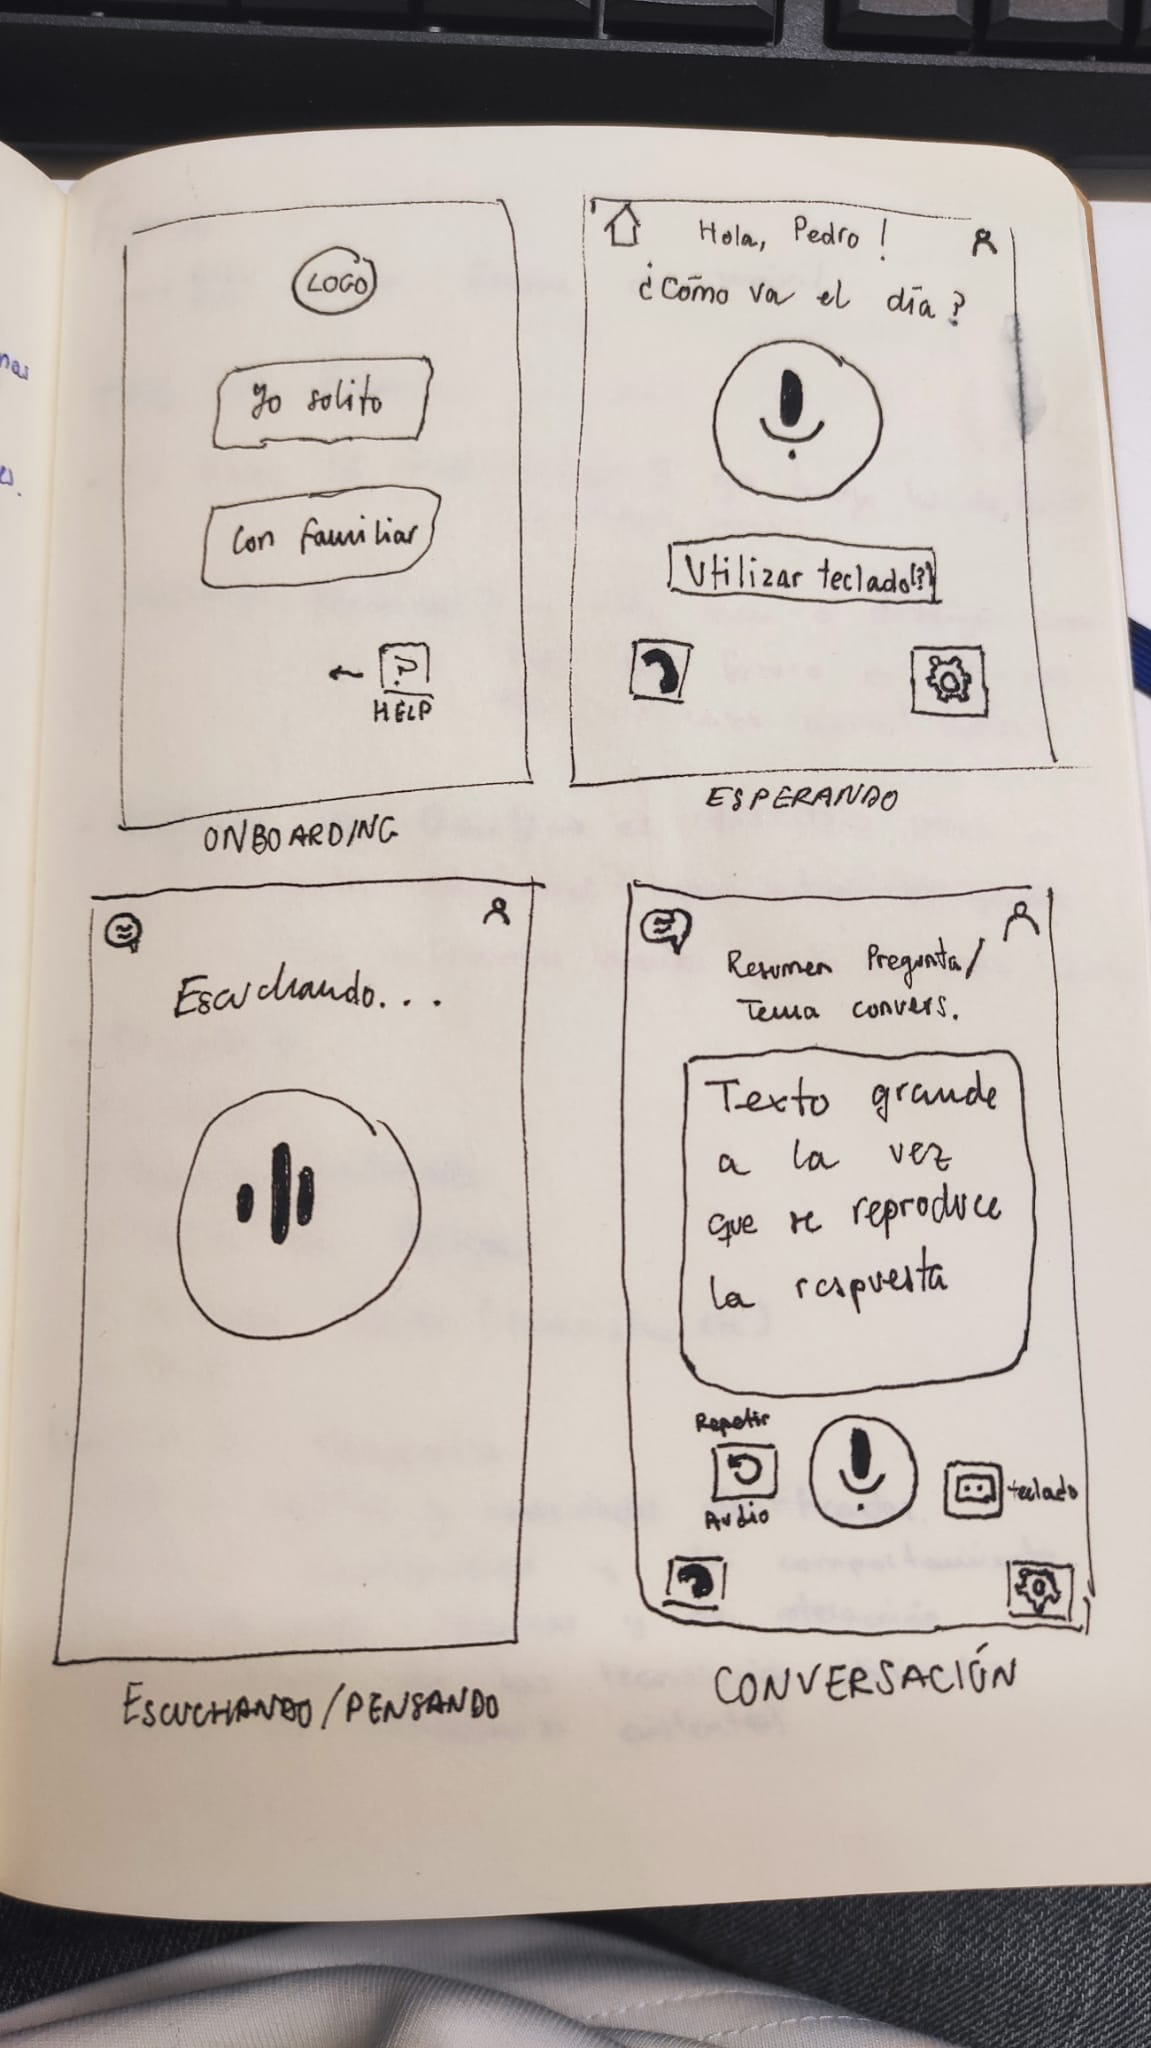
\includegraphics[height=11.5cm, trim={100 160 40 140}, clip]{imagenes/bocetos/boceto_mano_generico.jpeg}
  \caption[Bocetos a mano de los cuatro estados de la interfaz del mayor.]{Bocetos iniciales a mano de los cuatro estados de la interfaz del mayor: selección de autonomía, espera, escucha y conversación.}
  \label{fig:boceto-libreta}
\end{figure}

\subsection{Wireframes en Canva}

\begin{figure}[!tbp]\centering
  \begin{subfigure}[t]{0.3\textwidth}\centering
    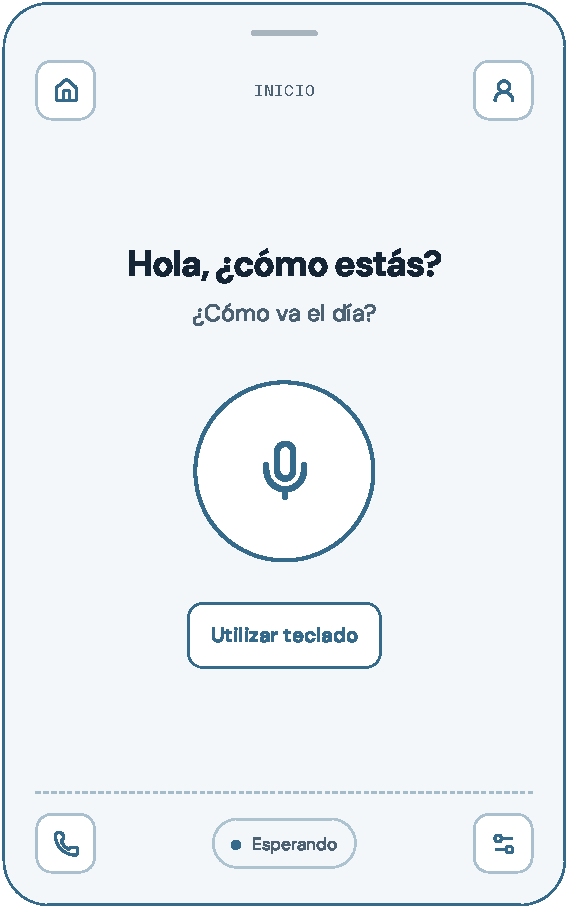
\includegraphics[width=\linewidth]{imagenes/bocetos/canva-1-inicio}
    \caption{Azul calmado}
  \end{subfigure}\hfill
  \begin{subfigure}[t]{0.3\textwidth}\centering
    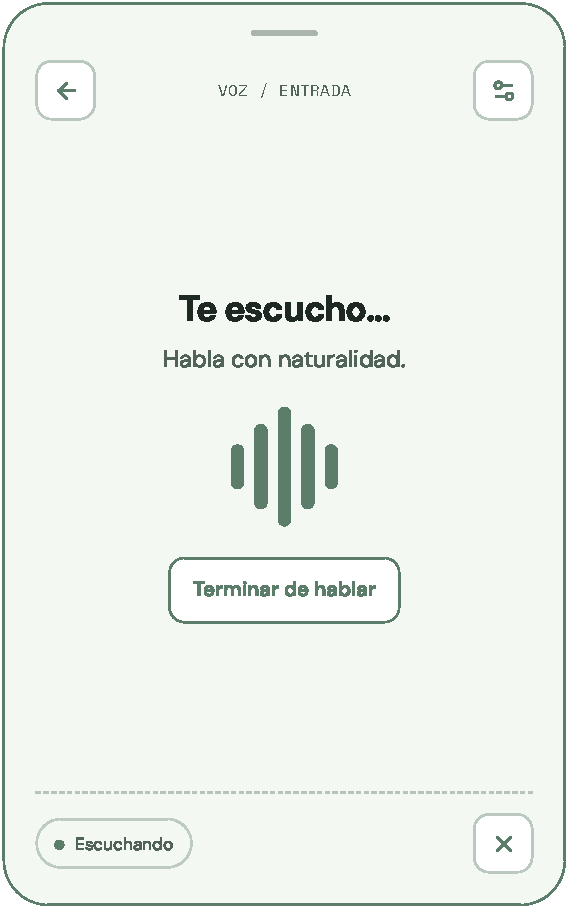
\includegraphics[width=\linewidth]{imagenes/bocetos/canva-2-escuchando}
    \caption{Verde salvia}
  \end{subfigure}\hfill
  \begin{subfigure}[t]{0.3\textwidth}\centering
    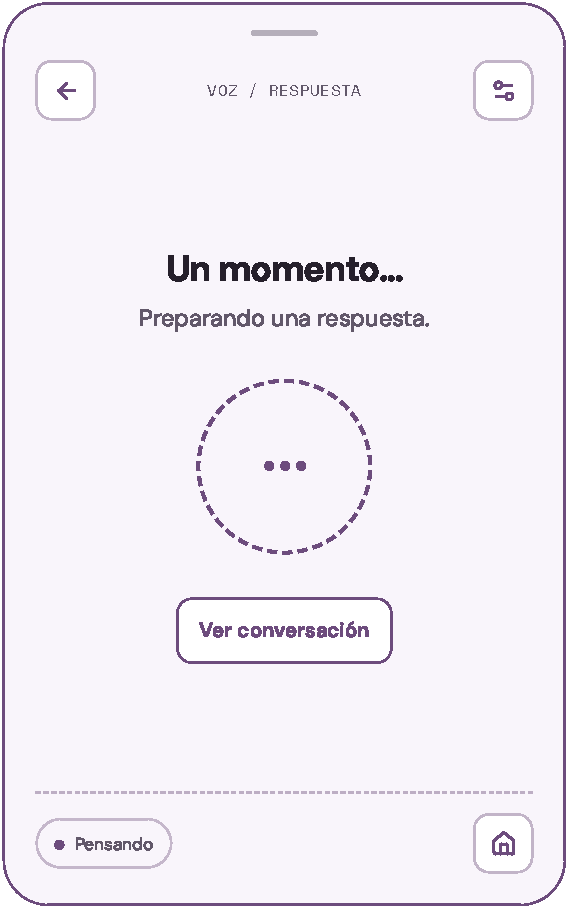
\includegraphics[width=\linewidth]{imagenes/bocetos/canva-3-procesando}
    \caption{Ciruela suave}
  \end{subfigure}

  \medskip
  \begin{subfigure}[t]{0.3\textwidth}\centering
    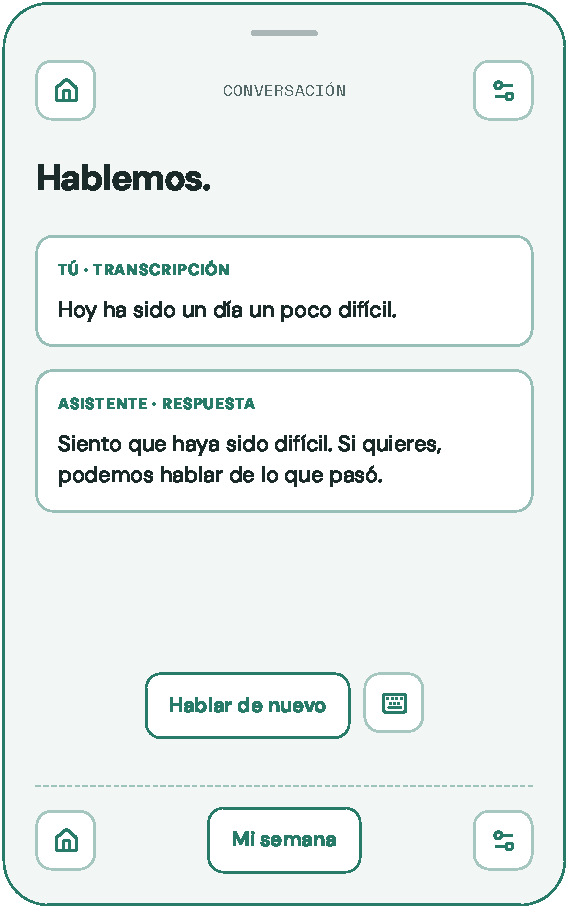
\includegraphics[width=\linewidth]{imagenes/bocetos/canva-4-conversacion}
    \caption{Azul petróleo}
  \end{subfigure}\hfill
  \begin{subfigure}[t]{0.3\textwidth}\centering
    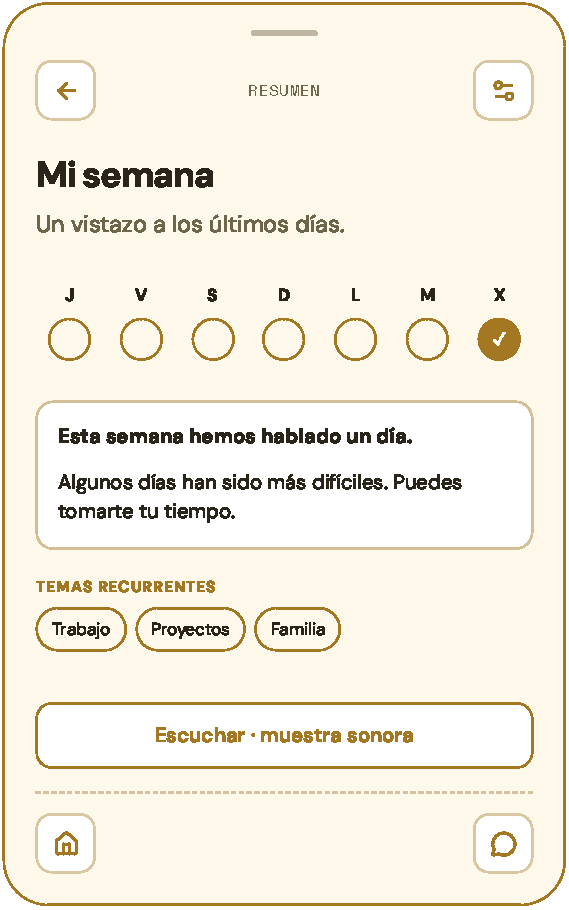
\includegraphics[width=\linewidth]{imagenes/bocetos/canva-5-mi-semana}
    \caption{Mostaza apagado}
  \end{subfigure}\hfill
  \begin{subfigure}[t]{0.3\textwidth}\centering
    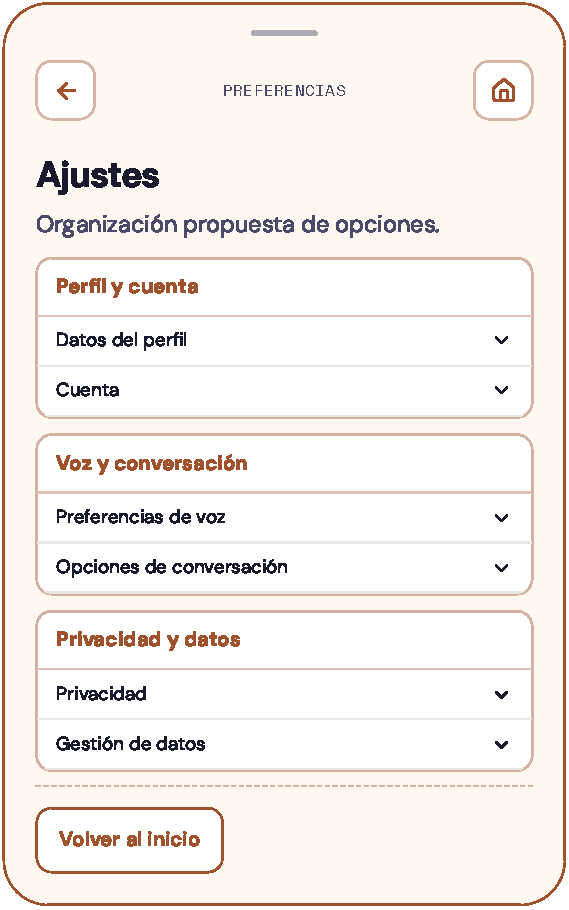
\includegraphics[width=\linewidth]{imagenes/bocetos/canva-6-ajustes}
    \caption{Canela, la elegida}
  \end{subfigure}
  \caption[Bocetos en Canva: una paleta candidata por pantalla.]{Bocetos en Canva del flujo del mayor (espera, escucha, procesamiento, conversación, <<Mi semana>> y Ajustes), cada pantalla con una de las paletas candidatas. La de Ajustes es la que adopta la aplicación.}
  \label{fig:bocetos-canva}
\end{figure}

La segunda etapa trasladó los bocetos supervivientes a wireframes digitales a escala, dibujados en Canva, y aportó la proporción: con las medidas reales, las restricciones de accesibilidad se ven como espacio ocupado. Un botón de 88~px de alto y un cuerpo de texto de 24~sp consumen enseguida la pantalla de un teléfono de gama media. El wireframe hace evidente que no caben seis opciones y obliga a decidir cuáles son las dos que importan.

La paleta de colores se decidió sobre una serie de bocetos en Canva que recorren el flujo completo del mayor, de la espera a Ajustes, con una paleta candidata distinta en cada pantalla y la misma composición en todas (\autoref{fig:bocetos-canva}). Se probaron cinco gamas (azul calmado, verde salvia, ciruela suave, azul petróleo y mostaza apagado) frente a la cálida, y se juzgaron con los dos criterios del apartado~\ref{sec:color}. El azul, el ciruela y el petróleo superan el 4{,}5:1 sobre su fondo, pero son tonos fríos, la zona del espectro que el cristalino envejecido filtra; el verde salvia (4{,}25:1) y la mostaza (3{,}82:1) no llegan a ese umbral. Solo Canela sobre blanco cálido cumple los dos, con 5{,}33:1.

\partesep{Parte II: Desarrollo}

\section{Stack tecnológico}
\label{sec:stack}

El sistema es una aplicación cliente Flutter (Dart, SDK \texttt{\textasciicircum 3.7.2}) compilada para Android (\code{minSdk} 24, \code{compileSdk} 36) apoyada en Firebase como \emph{Backend-as-a-Service}, en un conjunto de funciones propias desplegadas en Cloud Functions y en dos servicios de Google Cloud consumidos como API: Gemini, para la conversación y para el análisis de cada conversación al cerrarse, y Cloud Text-to-Speech, para la voz. La \autoref{tab:stack} recoge sus componentes.

\begin{table}[htbp]
    \centering
    \caption{Stack tecnológico en uso, con las versiones fijadas en \texttt{pubspec.yaml} y en el \texttt{package.json} de las funciones.}
    \label{tab:stack}
    \begin{tabularx}{\textwidth}{@{}l l >{\RaggedRight\arraybackslash}X@{}}
        \toprule
        \textbf{Capa} & \textbf{Componente} & \textbf{Función en el sistema} \\
        \midrule
        Cliente     & Flutter / Dart               & Interfaz nativa Android; sistema de diseño accesible propio \\
                    & \texttt{flutter\_riverpod} 2.5.1 & Estado reactivo e inyección de dependencias \\
                    & \texttt{go\_router} 17.0.0   & Enrutado declarativo con \emph{redirects} reactivos \\
                    & \texttt{speech\_to\_text} 7.3.0 & Transcripción de voz a texto (es-ES) \\
                    & \texttt{flutter\_tts} 4.2.5  & Síntesis de voz del dispositivo (respaldo) \\
                    & \texttt{just\_audio} 0.10.6  & Reproducción del audio sintetizado en la nube \\
                    & \texttt{url\_launcher} 6.3.2 & Apertura del marcador del sistema (emergencia) \\
                    & \texttt{permission\_handler} 12.0.1 & Permiso de micrófono \\
        \midrule
        Backend     & \texttt{firebase\_core} 3.15.2 & Inicialización del SDK \\
                    & \texttt{firebase\_auth} 5.7.0  & Autenticación dual (Google o anónima / correo) \\
                    & \texttt{google\_sign\_in} 7.2.0 & Selector de cuentas de Google del mayor \\
                    & \texttt{cloud\_firestore} 5.6.0 & Persistencia y sincronización en tiempo real \\
                    & \texttt{cloud\_functions} 5.4.0 & Cliente de las cinco \emph{callables} \\
                    & Cloud Functions (Node 22, gen 2) & Lógica de servidor (\autoref{tab:callables}) \\
        \midrule
        Servicios   & Vertex AI (\texttt{@google/genai}) & Gemini \texttt{gemini-2.5-flash} en el servidor: conversación, análisis y memoria \\
                    & Cloud Text-to-Speech           & Cuatro voces Chirp~3:~HD en español, a elegir \\
        \bottomrule
    \end{tabularx}

\end{table}

Las cuatro elecciones principales responden a dos restricciones: un único desarrollador con plazo ajustado y alta carga de trabajo, y un usuario cuyas limitaciones exigen controlar la interfaz por completo.

\textbf{Flutter} permite mantener una sola base de código, en lugar de una por plataforma, y dibuja su propia interfaz sin depender de los componentes del sistema operativo, que es lo que exige un sistema de diseño accesible redefinido por completo. Una aplicación web habría compartido la primera ventaja, pero con un acceso al micrófono más limitado. iOS es una plataforma posible pero no verificada.

\textbf{La inteligencia conversacional se delega en un LLM en la nube}, Gemini \code{gemini-2.5-flash}. Un modelo local exigiría inferencia neuronal a los terminales de gama media y baja a los que se dirige la aplicación, y ajustar un modelo propio era inviable sin datos conversacionales. Gemini comparte proyecto y facturación con Firebase y Cloud Text-to-Speech, tiene un coste despreciable a la escala de las pruebas (apartado~\ref{sec:costes}) y admite la invocación de funciones, con la que el asistente guarda el nombre del mayor en cuanto lo oye. El tono empático se consigue con la instrucción de sistema y los filtros de seguridad que fija en el servidor la función \code{chatTurn}.

\textbf{Firebase} resuelve lo que un desarrollador único no podría construir y operar a la vez: autenticación, persistencia y, sobre todo, la sincronización en tiempo real entre el dispositivo del mayor y el de su familiar, sin la que el modelo dual no existe. Sus \emph{streams} de documento son además la base de la fuente única de verdad (apartado~\ref{sec:ssot}). Donde el cliente no basta, el BaaS se completa con funciones propias (apartado~\ref{sec:paas}).

\textbf{Riverpod} cubre con un solo mecanismo el estado reactivo y la inyección de dependencias, y su \code{StreamProvider} encaja con los \emph{snapshots} de Firestore; la combinación habitual de BLoC con un localizador de servicios exige dos piezas para lo mismo. Se mantiene en la línea 2.x por un conflicto de la 3.x con \code{scheduleNewFrame} en el entorno de desarrollo Linux empleado, y todo el ecosistema FlutterFire se alinea sobre \code{firebase\_core} 3.x para evitar conflictos de dependencias transitivas: ambas fijaciones persiguen la reproducibilidad del \emph{build}.

\section{Arquitectura}
\label{sec:arquitectura}

\subsection{Visión general del sistema}
\label{sec:arquitectura-general}

La \autoref{fig:arquitectura} sitúa las piezas del sistema y cómo se comunican. Cada número de la figura identifica un flujo y cada letra, el orden de sus pasos; la flecha parte de quien inicia la operación.

El mayor y el familiar ejecutan la misma aplicación, que se comporta de una u otra forma según el rol almacenado en el perfil (revelación progresiva). Ambos se autentican contra Firebase Authentication (flujo~1), el mayor con su cuenta de Google o sin registrarse y el familiar con correo y contraseña, y ambos observan la colección \code{users} de Cloud Firestore (flujo~7), que actúa como memoria compartida entre los dos dispositivos y como mecanismo de propagación en tiempo real de las preferencias.

El ciclo conversacional ocupa los flujos~2 y~3. La voz la transcribe el reconocedor del propio Android, y la aplicación recibe solo el texto: no graba ni guarda el audio. El texto viaja a la \emph{callable} \code{chatTurn}, que lee del perfil el nombre del mayor y, si ha consentido guardar sus conversaciones, su memoria, y pide la respuesta a Gemini a través de Vertex AI; si el mayor dice cómo se llama, es la propia función quien guarda el nombre. La respuesta se trocea en frases, y cada una se envía a la \emph{callable} \code{synthesizeSpeech}, que llama a la API de Cloud Text-to-Speech con la voz elegida por el mayor y devuelve el audio. El reproductor del cliente lo reproduce con el volumen y la velocidad configurados y, si la síntesis de una frase falla o tarda demasiado, esa frase y las siguientes las pronuncia el motor de voz del dispositivo. Cuando el mayor prefiere escribir, el texto tecleado ocupa el lugar de la transcripción y la cadena es la misma, salvo que la respuesta solo se lee si él lo pide (apartado~\ref{sec:teclado}).


Al cerrarse cada conversación (flujo~4), el cliente entrega lo hablado a \code{closeConversation}, que comprueba en el perfil el consentimiento y el plazo de conservación, lo analiza con Gemini, guarda únicamente el resultado y descarta el texto. Ese resultado llega después a los dos dispositivos por Firestore, como cualquier otro dato. El emparejamiento (flujo~5) no se resuelve contra Firestore desde el cliente, sino a través de la \emph{callable} \code{validateAndLink}, que localiza al mayor por su código con credenciales de administrador y actualiza ambos perfiles en una única transacción. Y el consentimiento del mayor sobre sus conversaciones (flujo~6) solo puede escribirse a través de \code{setConversationConsent}. La llamada de emergencia (flujo~8), en cambio, no atraviesa el \emph{backend} en absoluto: construye un URI \code{tel:} y cede el control al marcador del sistema operativo. Por último, las reglas de seguridad de Firestore, la banda vertical de la figura, se interponen en todo acceso de cliente a la base de datos, de manera que ni siquiera un binario modificado puede leer o escribir fuera de lo que esas reglas permiten.


\afterpage{%
\begin{landscape}
\begin{figure}[p]\centering
  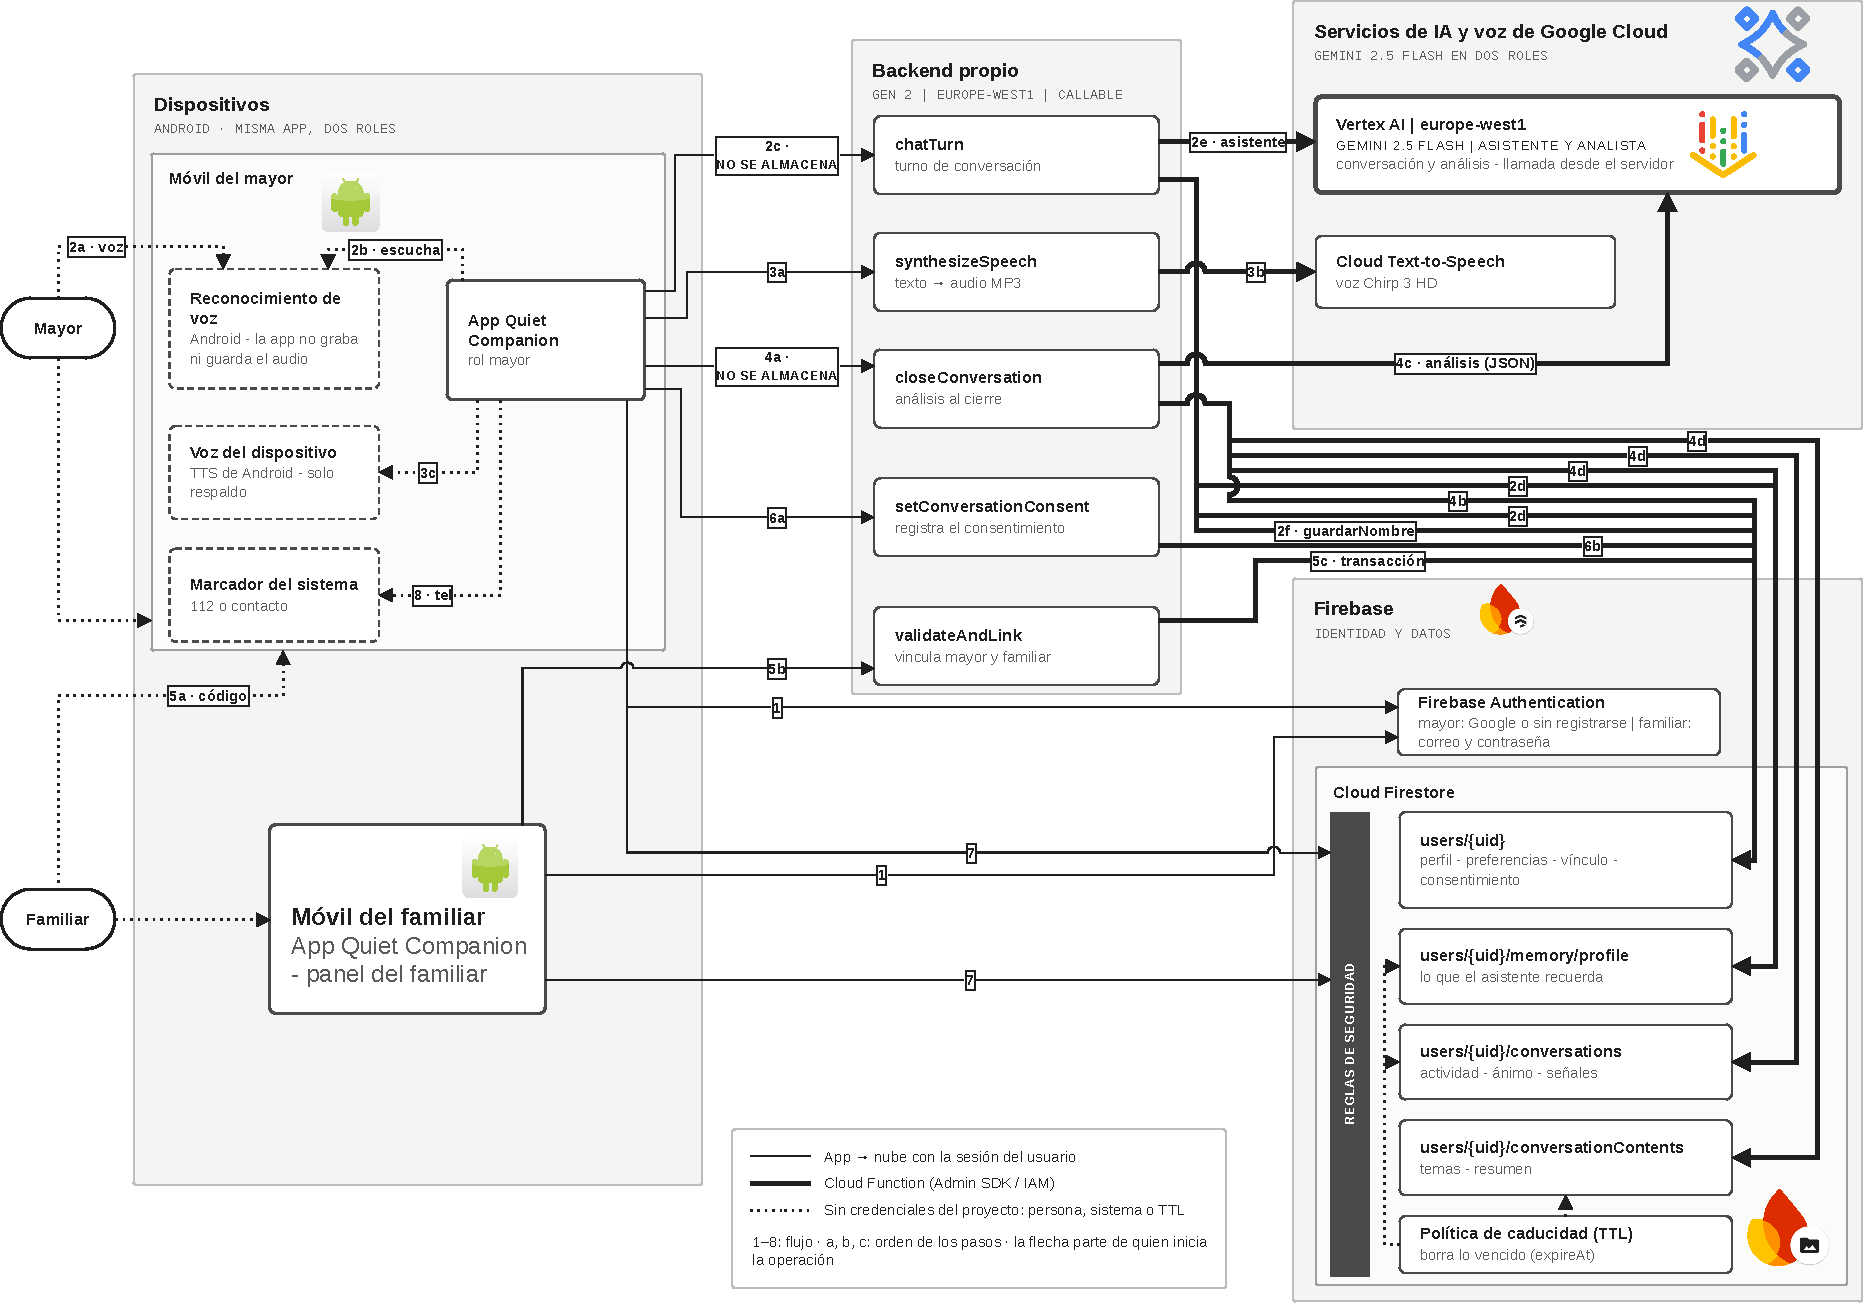
\includegraphics[width=\linewidth, height=\dimexpr\textheight-3\baselineskip\relax, keepaspectratio]{imagenes/arquitectura/arquitectura_sistema.pdf}
  \caption{Arquitectura del sistema: dispositivos, servicios gestionados y flujos de datos.}
  \label{fig:arquitectura}

  \vspace{2pt}
  {\footnotesize Fuente: Elaboración propia.}
\end{figure}
\end{landscape}}

Los servicios de pago, Gemini y Cloud Text-to-Speech, solo se alcanzan a través del \emph{backend} propio, de modo que el teléfono no guarda credenciales de ninguno de ellos; lo que el teléfono resuelve por sí solo, el reconocimiento de voz, la voz de respaldo y la llamada de emergencia, no sale de él; y el resto es acceso directo a Firestore, acotado por las reglas (apartado~\ref{sec:seguridad}).


\subsection[El servidor como plataforma gestionada: Firebase y Cloud Functions]{El servidor como plataforma gestionada: Firebase y\\ Cloud Functions}
\label{sec:paas}

Que el sistema tenga servidor propio no significa que el proyecto opere un servidor. Gracias a esa diferencia, un único desarrollador puede tener un \emph{backend} con lógica propia. El NIST define la plataforma como servicio (PaaS) como la capacidad de desplegar en la infraestructura del proveedor aplicaciones propias, escritas con los lenguajes y herramientas que este admite, sin gestionar ni controlar la red, los servidores, el sistema operativo ni el almacenamiento subyacentes: el cliente controla solo la aplicación desplegada y, en su caso, la configuración del entorno que la aloja \citep{NIST800145}. Quiet Companion combina dos variantes de ese modelo. Firebase actúa como \emph{Backend-as-a-Service}: la autenticación y la base de datos se consumen ya construidas, a través del SDK del cliente. Cloud Functions es una plataforma de funciones (\emph{Function-as-a-Service}), la forma más acotada de PaaS, en la que la unidad de despliegue es una función que el proveedor ejecuta bajo demanda, escala desde cero instancias y factura por invocación, de modo que el desarrollador no administra máquina alguna \citep{Jonas2019}. En la segunda generación, que es la que usa el proyecto, cada función se construye con Cloud Build y se despliega como un servicio de Cloud Run \citep{FirebaseFunctionsVersions}.

Un BaaS basta mientras toda la lógica pueda vivir en el cliente, y hay tres cosas que un cliente no puede hacer por sí solo. La primera es \textbf{guardar un secreto}: cualquier credencial empaquetada en la aplicación puede extraerse del binario, y la síntesis de voz y el análisis necesitan credenciales de Google Cloud (RNF-8). La segunda es \textbf{actuar sobre datos ajenos sin abrirlos a todos}: las reglas de Firestore autorizan operaciones enteras y no ven las cláusulas de una consulta, de modo que lo que exige buscar o escribir fuera del documento propio, como la vinculación, solo es seguro con privilegios de servidor (RNF-9). La tercera es \textbf{dar fe}: la hora de un consentimiento, la comprobación de que existe antes de analizar nada o el tope del plazo de conservación no pueden depender de lo que declare un dispositivo que controla el propio usuario. Esas necesidades se traducen en funciones propias, y la \autoref{tab:callables} recoge las cinco que componen el \emph{backend}.

Las cinco funciones son \emph{callables} (\code{onCall}) y no funciones HTTP genéricas ni disparadores de base de datos: el SDK de Firebase adjunta y verifica el token de sesión en cada invocación, de modo que el servidor toma la identidad de quien llama de \code{request.auth} y nunca de un parámetro, y nadie puede pedir que se actúe en nombre de otro. Un disparador no servía para el análisis, porque habría exigido escribir antes la transcripción en Firestore. Todas se despliegan en \code{europe-west1}, junto a los datos, con un tope de diez instancias como salvaguarda de coste en un proyecto sin financiación, y ninguna maneja claves: se autentican ante Cloud Text-to-Speech y Vertex AI con las credenciales por defecto de la cuenta de servicio del entorno. La lógica que decide (validar la entrada, sanear la respuesta del modelo, aplicar los cambios de memoria o calcular cuándo caduca un dato) vive en módulos puros separados de los manejadores, y se prueba con \code{node --test} sin emulador ni red, en veintitrés casos. Los registros contienen longitudes e identificadores, nunca texto de una conversación.

\begin{table}[htbp]
    \centering
    \caption{Funciones del \emph{backend}, todas \emph{callables} desplegadas en \texttt{europe-west1}.}
    \label{tab:callables}
    \small
    \begin{tabularx}{\textwidth}{@{}l >{\RaggedRight\arraybackslash}X >{\RaggedRight\arraybackslash}X@{}}
        \toprule
        \textbf{Función} & \textbf{Qué hace} & \textbf{Por qué en el servidor} \\
        \midrule
        \texttt{chatTurn}               & Responde cada turno de la conversación y guarda el nombre del mayor cuando lo dice & Gemini sin clave; el servidor fija las instrucciones del asistente y solo lee la memoria si hay consentimiento \\
        \addlinespace
        \texttt{synthesizeSpeech}       & Convierte una frase en audio con la voz Chirp~3:~HD elegida & Las credenciales de Cloud TTS no salen del servidor, único que conoce los nombres de las voces \\
        \addlinespace
        \texttt{validateAndLink}        & Vincula mayor y familiar por el código, en una transacción & Busca por código con privilegios de administrador sin que \texttt{/users} sea enumerable \\
        \addlinespace
        \texttt{setConversationConsent} & Registra o retira el consentimiento del mayor & La hora del servidor es la prueba; programa el borrado de lo guardado \\
        \addlinespace
        \texttt{closeConversation}      & Analiza la conversación al cerrarse y actualiza la memoria & Gemini sin clave; la transcripción no se almacena; aplica los plazos \\
        \bottomrule
    \end{tabularx}

\end{table}


La mayor ventaja de la plataforma está en el proceso. Un cambio en el \emph{prompt} del análisis o en la voz se publica con \code{firebase deploy}, sin generar ni instalar una APK nueva, y cada análisis guarda la versión del \emph{prompt} que lo produjo. A cambio, la primera invocación tras un periodo sin uso paga el arranque en frío de la instancia, que en la voz cubre el respaldo al motor del dispositivo, y el proyecto queda ligado a la plataforma de Google, una dependencia ya asumida al elegir Firebase.

\subsection{Estructura core/ y features/, y capas por \emph{slice}}

El código se organiza según el modelo híbrido Clean Feature-Sliced (CFS) prescrito por RNF-11: rebanadas verticales de funcionalidad sobre un núcleo transversal. Frente a la organización por capas técnicas, que reparte cada funcionalidad entre varias carpetas, CFS agrupa por funcionalidad; añade una regla explícita contra el acoplamiento lateral, y renuncia a las capas adicionales de Feature-Sliced Design estricto, desproporcionadas para el tamaño del proyecto. Dentro de cada rebanada se usa la nomenclatura de Clean Architecture, conocida por cualquier desarrollador.

\begin{lstlisting}[style=Consola, float=!tbp, caption={Estructura real del árbol de código fuente.}, label={lst:arbol}]
lib/
|-- core/                 # lo que comparten dos o más features
|   |-- config/           # router, redirect, filas de ajustes, plazos
|   |-- constants/        # firestore_paths
|   |-- models/           # usuario, consentimiento, conversación...
|   |-- providers/        # currentUserProvider, linkedElderProvider...
|   |-- repositories/     # autenticación, conversaciones y memoria
|   |-- services/         # Gemini, voz (STT y TTS), cierre...
|   |-- theme/            # AppTheme
|   |-- utils/            # sentence_splitter, week_summary
|   `-- widgets/          # ElderButton, SignOutButton
|-- features/
|   |-- conversation/  {data, domain, presentation}
|   |-- dashboard/     {domain, presentation}
|   |-- emergency/     {presentation}
|   |-- my_week/       {domain, presentation}
|   |-- onboarding/    {domain, presentation}
|   |-- privacy/       {data, domain, presentation}
|   `-- settings/      {presentation}
`-- main.dart, firebase_options.dart
functions/                # index.js (5 callables) y lógica pura
firestore.rules, firestore-tests/
\end{lstlisting}

Una \emph{feature} no importa nunca de otra, es decir, no hay acoplamiento horizontal, y lo compartido va a \code{core/}. El único punto de \code{core/} que conoce las \emph{features} es el enrutador, que compone sus pantallas.

Un ejemplo claro es \code{settings\_rows.dart}. Las filas de la pantalla de ajustes viven en \code{core/config/} y no en \code{features/settings/}, aunque intuitivamente pertenezcan a esa \emph{feature}, porque las consumen dos \emph{features} que no pueden acoplarse entre sí: \code{conversation} decide con ellas si muestra el botón de Ajustes, y \code{settings} decide qué muestra. Ubicar la lista en cualquiera de las dos habría obligado a la otra a importarla. Por la misma razón, la agregación semanal que muestran el panel del familiar y <<Mi semana>> vive en \code{core/utils/week\_summary.dart}, y el repositorio de autenticación, que usan el \emph{onboarding}, el panel, Ajustes y el contacto de emergencia, en \code{core/repositories/}.

\code{emergency} y \code{settings} tienen solo \code{presentation} porque su lógica se resuelve con servicios de \code{core/} y funciones puras, sin estado propio, y una carpeta \code{domain} vacía por simetría sería complicarlo sin necesidad.

\subsection{Single Source of Truth: \texttt{currentUserProvider}}
\label{sec:ssot}

Varias partes del sistema necesitan el documento \code{users/{\char123}uid{\char125}} en tiempo real: el enrutador para decidir redirecciones, la pantalla principal para el tamaño de letra, el servicio de voz para el volumen y la velocidad, y el panel del familiar. Que cada uno abriese su propia suscripción a Firestore duplicaría escuchas y repartiría la responsabilidad de mantener el dato.

La arquitectura adopta un \textbf{único punto de escucha}. \code{firebaseAuthUserProvider} emite el usuario de Firebase Auth; \code{currentUserProvider} lo observa y, cuando hay sesión, se suscribe a \code{users/{\char123}uid{\char125}} y lo mapea a \code{UserModel}. Cualquier widget o controlador, en cualquier punto de la aplicación, se limita a observar ese proveedor con \code{ref.watch}, y Riverpod reconstruye solo a quienes lo observan cuando Firestore emite.

Cuando el familiar completa el emparejamiento, la transacción borra el \code{linkCode} del documento del mayor; el \emph{stream} emite, el enrutador recalcula su decisión y el dispositivo del mayor avanza solo a la pantalla siguiente, sin que el mayor pulse nada. El mismo mecanismo propaga en caliente, sin código adicional, las preferencias de accesibilidad (RF-6).

El panel del familiar aplica el mismo patrón al documento del mayor: \code{linkedElderProvider} es para el familiar lo que \code{currentUserProvider} es para el propio usuario. El panel pinta desde ese \emph{stream} y cada control escribe solo su campo, con una ruta de punto (\code{preferences.volume}), nunca el documento entero. Es lo que permite que el mayor y su familiar modifiquen el mismo documento sin pisarse: el mayor ajusta sus escalas y el asistente aprende su nombre, y ningún deslizador del familiar puede revertirlo. Cada deslizador escribe en \code{onChangeEnd}, una vez por gesto y no decenas de veces por segundo, y la actualización es optimista: si la escritura falla, la propia caché de Firestore devuelve el control a su valor real, en lugar de dejar en pantalla uno que nunca llegó a guardarse.

\subsection{Gestión de estado e inyección de dependencias}
\label{sec:estado-di}

Todo estado de negocio se modela como un \code{StateNotifier} sobre una clase de estado inmutable con \code{copyWith}. No se usa \code{setState} para lógica de negocio en ningún punto; las pantallas son \code{ConsumerWidget} o \code{ConsumerStatefulWidget} que observan y dibujan. El único estado local admitido en la capa de presentación es el estrictamente efímero de un widget: la posición de un deslizador mientras se arrastra, la posición de un \code{ScrollController}.

Riverpod cubre simultáneamente el estado reactivo y la inyección de dependencias (RNF-12): servicios y repositorios se resuelven vía \code{Provider} y se pasan por constructor, nunca se instancian dentro de la clase que los usa. Gracias a ello, los tests de la pantalla de emergencia sustituyen \code{TtsService}, \code{SpeechService} y \code{EmergencyCallService} por falsos sin tocar los \emph{plugins} reales, y el controlador del chat recibe todos sus servicios por constructor.

\subsection{Operaciones atómicas y enrutado reactivo}

El emparejamiento entre mayor y familiar exige modificar dos documentos de usuarios distintos sin que pueda quedar un estado intermedio en el que uno esté vinculado y el otro no. Se resuelve con una transacción de Firestore, ejecutada en el servidor dentro de \code{validateAndLink} (apartado~\ref{sec:seguridad}), que revalida el código y actualiza ambos documentos en una sola operación. Es una transacción y no un lote de escritura (\code{WriteBatch}) porque necesita \emph{leer}: el contacto de emergencia del familiar se copia al mayor solo si este no ha fijado uno a mano, y eso exige leer antes su documento.

\code{RouterNotifier} observa los dos controladores de autenticación, el estado de Firebase Auth y \code{currentUserProvider}, y notifica a \code{go\_router} en cada cambio para que recalcule la redirección. La decisión de destino se toma sobre el dato en vivo del proveedor, con el estado del controlador únicamente como respaldo durante el intervalo previo a la primera emisión del \emph{stream}, y una guarda de rol impide que el documento de un familiar se use para decidir la ruta de un mayor. Esa decisión vive en una función pura, \code{routeRedirect}, extraída para que las pruebas del enrutador cubran la lógica real y no una copia escrita a mano. La misma función envía a \code{/consent}, antes de la pantalla principal, al mayor ya dado de alta que nunca ha respondido a la pregunta del consentimiento (apartado~\ref{sec:privacidad}).

\section{Seguridad: identidad, vinculación y reglas}
\label{sec:seguridad}

La seguridad del sistema descansa en tres piezas: cómo se identifica cada actor, cómo se vinculan mayor y familiar sin exponer a terceros, y qué reglas protegen cada acceso a la base de datos.

\textbf{Autenticación dual.} El familiar usa correo y contraseña, porque necesita una cuenta portable. Al mayor, escribir un correo y una contraseña le supondría una barrera real, así que la bienvenida le ofrece dos vías del mismo peso: \textbf{su cuenta de Google}, que se elige sin escribir nada, o \textbf{entrar sin registrarse}, con una sesión anónima. Ni el perfil ni las reglas distinguen cómo ha entrado, porque las dos vías dan un identificador de Firebase del mismo tipo. La sesión anónima no ofrece cierre de sesión, porque cerrarla o reinstalar la aplicación generaría un identificador nuevo y perdería el perfil; por eso <<Mi cuenta>> permite guardarla después con Google sin cambiar de identificador, y la memoria, las conversaciones y el vínculo con el familiar se conservan. La cuenta de Google de un familiar no sirve para entrar como mayor: la aplicación cierra la sesión antes de que elegir modo le reescriba el rol.

\textbf{Vinculación en el servidor.} El mayor que elige el modo vinculado recibe un código de cuatro caracteres, sin símbolos confundibles, que su familiar introduce en su propia aplicación. Encontrar al mayor a partir de ese código es una consulta de colección (\code{where('linkCode', '==', code)}), y las reglas de Firestore no ven las cláusulas de una consulta: solo pueden permitir o denegar la operación entera. Si la búsqueda se hiciera desde el cliente, \code{/users} tendría que ser consultable por cualquier usuario autenticado, y cualquiera con la aplicación instalada podría enumerar el directorio de usuarios, con sus nombres y sus teléfonos de contacto. Por eso la vinculación es una \emph{callable}, \code{validateAndLink}. La búsqueda corre con credenciales de administrador, lo que permite denegar a todo cliente el listado de \code{/users}; el identificador del familiar lo toma el servidor de la sesión autenticada y no de un parámetro, así que nadie puede vincular a un tercero; el servidor comprueba que quien vincula es realmente un familiar registrado; y el código se consume dentro de la misma transacción que lo valida, por lo que solo sirve una vez. Así se cumple RNF-9.

\textbf{Reglas que modelan el código real.} Las reglas de Firestore describen operación por operación lo que hace la aplicación: lectura solo por identificador, para el dueño y para el familiar vinculado; borrado siempre denegado; escritura del familiar acotada por campo a las preferencias, el nombre y los plazos de la conversación, de modo que el panel no puede cambiar el rol del mayor, romperle el vínculo, reescribirle el contacto de emergencia ni decidir sobre su consentimiento; y denegación por defecto para todo lo demás. Las reglas no admiten nada que la aplicación no haga: si una operación cambia y las reglas no la contemplan, se muestra un error y las pruebas lo señalan, en vez de que las reglas queden desfasadas sin que nadie lo note.

\textbf{Reglas verificadas contra el emulador.} Cuando una regla falla, el error aparece en el dispositivo del usuario y no en el del desarrollador. Por eso se prueban contra el emulador de Firestore, con doce casos agrupados por sujeto (el dueño, el familiar vinculado y un autenticado cualquiera) y por garantía (que \code{/users} no sea enumerable, que el consentimiento y el análisis solo los escriba el servidor y que el familiar vea solo lo que el mayor elige). Son las únicas pruebas del proyecto que comprueban lo que el sistema debe rechazar a quien no usa la aplicación.

\textbf{Ninguna credencial en el teléfono.} La conversación en vivo pasa por \code{chatTurn}, que llama a Gemini a través de Vertex AI con las credenciales de la cuenta de servicio, igual que el análisis al cierre, de modo que el binario no contiene credenciales de ningún servicio de pago y RNF-8 se cumple. La función compone además las instrucciones del asistente y sus filtros de seguridad, que un cliente modificado no puede sustituir, y acota la longitud de cada turno y del historial que recibe. El precio es un salto de red más por turno en el camino que más se usa, el de la respuesta en vivo.


\section{La voz}
\label{sec:voz}

La voz es la interfaz primaria del mayor, y de su calidad, su ritmo y su turno depende que la conversación resulte natural.

\textbf{Síntesis en la nube.} El motor de voz nativo de Android produce una voz perceptiblemente robótica, cuya calidad depende además del motor instalado en cada dispositivo, y para una población mayor una voz poco natural reduce la inteligibilidad y la disposición a conversar. Por eso la voz se sintetiza en el servidor, con Cloud Text-to-Speech y las voces Chirp~3:~HD en español de España, del mismo proveedor que el resto del sistema. Dos mecanismos la hacen viable en una conversación: el \textbf{troceado por frases}, que sintetiza la primera oración y la reproduce mientras se sintetiza la siguiente, de modo que el primer audio llega tras un solo viaje de red; y el \textbf{respaldo sin reintentos}: si la síntesis de una frase falla o tarda, esa frase y las siguientes se pronuncian con el motor del dispositivo, porque para este usuario una voz peor pero inmediata es preferible a un silencio imprevisible.

\textbf{Una voz a elegir.} El mayor elige entre cuatro, dos de mujer y dos de hombre: las del catálogo Chirp~3:~HD que Google describe con el registro de un acompañante (cálida, dulce, amable y suave). No son más porque se comparan de oído, y con más opciones ya no se recuerda cómo sonaba la primera. Cada una se presenta por cómo suena (<<Voz de hombre, amable>>) y no por su nombre de catálogo, y al tocarla se guarda y dice una frase de muestra, sin botón de guardar, como las escalas. El familiar puede elegirla también desde el panel, tras escuchar cada opción. La voz por omisión es masculina porque, en los terminales probados, el motor del dispositivo habla con voz de mujer, y así el respaldo se reconoce de oído.

\textbf{Preferencias aplicadas en el reproductor.} La función de síntesis recibe solo el texto y la clave de la voz, que traduce a su nombre real desde una lista cerrada: una clave desconocida suena con la voz por omisión, y nadie puede pedir una voz cualquiera ni colar parámetros de síntesis. Sintetiza siempre a ritmo neutro. El volumen y la velocidad elegidos los aplica el reproductor del cliente, con el mismo factor de conversión que \code{flutter\_tts} usa en Android, y así el ajuste significa lo mismo con la voz de la nube y con la de respaldo. \code{just\_audio} sirve el audio en memoria a través de un servidor HTTP local en \code{127.0.0.1}, y como Android prohíbe por defecto el tráfico en claro, la configuración de seguridad de red lo permite exclusivamente hacia esa dirección y no de forma global.

\textbf{Escucha por turnos.} El reconocedor de voz de Android corta su sesión en cada pausa, así que la aplicación encadena sesiones y da el turno por terminado tras un silencio, sin que el mayor tenga que pulsar nada. Cuánto silencio basta depende de la persona, que puede detenerse a pensar a mitad de una idea. Por eso no es una constante sino una escala más de Ajustes, <<Tiempo que te espero>>, de dos a diez segundos y tres por omisión. Al cerrar cada sesión, la aplicación espera, con un tope de un segundo, al resultado final del reconocedor, porque Android avisa de que ha dejado de grabar antes de entregar el único resultado que contiene la última palabra.

\section{Conversación, memoria y seguimiento del bienestar}
\label{sec:conversacion}

Resumir una conversación, medir el ánimo o recordar exigen decidir antes qué es \emph{una conversación}. Sin una frontera, la sesión del modelo duraría lo que la aplicación abierta: con el teléfono encendido en un soporte, abarcaría la charla de la mañana y la de la noche, con un historial que crecería sin límite y se reenviaría entero en cada turno. Este apartado recorre las cuatro piezas que resuelven HU-5 y HU-6: la frontera de la conversación, su análisis al cerrarse, la memoria que de él se deriva y la presentación del resultado al mayor y a su familiar. En ninguna de las cuatro se almacena la transcripción.

\subsection{La conversación como unidad}

Una conversación empieza con el primer turno del mayor y termina con lo primero que ocurra de dos cosas: que pase un tiempo sin turnos, cinco minutos por omisión, contado desde que el asistente \emph{termina} de hablar para que una respuesta larga no consuma la ventana, o que la aplicación pase a segundo plano. Si el mayor sale hacia el marcador de emergencia, la conversación sigue abierta. No hay botón de <<terminar>>, porque sería una decisión más para el mayor y nadie da por terminada de forma explícita una charla con quien le acompaña, de modo que las conversaciones no se cerrarían nunca.

Mientras dura, la conversación vive solo en la memoria del teléfono: el controlador del chat acumula los turnos completos, con su autor y su hora, y excluye las respuestas de error de la propia aplicación, que no son conversación y sesgarían el análisis hacia lo negativo. Al cerrarse, el controlador entrega ese búfer al servidor sin que el mayor espere ni vea nada, lo vacía y deja preparada una sesión nueva del modelo para el turno siguiente. Si el mayor ha intervenido menos de tres veces, solo sale del dispositivo la constancia de la conversación, sin texto, porque un <<hola, adiós>> no tiene ánimo que medir. Y la escucha del ciclo de vida de la aplicación vive en el proveedor del chat y no en una pantalla, para que la conversación se cierre aunque el mayor esté en Ajustes al salir.

Si Android mata el proceso antes de que el envío llegue al servidor, el análisis de esa conversación se pierde. Guardar el búfer en disco para sobrevivir a esa muerte dejaría la transcripción en reposo en el dispositivo, justo lo que el diseño prohíbe. Como efecto secundario favorable, que la sesión del modelo coincida con la conversación acota el coste de cada turno, que deja de crecer con el tiempo que la aplicación lleve abierta.

\subsection{Análisis al cierre en el servidor}

Todo el análisis ocurre al cerrarse la conversación, en el servidor, por cuatro razones. Lo que no se guarda solo puede analizarse mientras existe, de modo que el análisis tiene que hacerse en el cierre. Analizar la transcripción, y no un resumen previo, es analizar las palabras del mayor y no una paráfrasis escrita para ser breve y neutra, en la que el afecto ya se ha perdido. Pasarla por una función propia que no la escribe no añade destinatario ni almacenamiento, porque la transcripción ya viaja a Google en cada turno. Y un \emph{prompt} en el servidor se ajusta sin publicar una APK nueva.

La realización es una sola \emph{callable}, \code{closeConversation}, que recibe la conversación terminada y hace una única llamada al modelo; la \autoref{fig:secuencia-cierre} recoge el recorrido completo. La función comprueba primero que quien llama es un mayor y que su consentimiento está vigente; si no lo está, rechaza la petición sin escribir nada, con independencia de que el cliente, que tampoco envía nada sin consentimiento, se haya comportado bien. Valida después la entrada, y cuenta ella misma los turnos del mayor en lugar de fiarse del número que declara el cliente. Y llama a \code{gemini-2.5-flash} a través de Vertex AI con \textbf{salida estructurada}: un esquema JSON con enumerados cerrados y temperatura baja, de modo que de una sola llamada salen a la vez el sentimiento, las señales, los temas, el resumen y los cambios de memoria. Tratar el texto una vez, y no una por dato, es también minimización. La respuesta se sanea antes de escribirse, porque lo que entra en la base de datos no puede depender de que el modelo cumpla el esquema <<casi siempre>>.

\begin{figure}[htbp]
    \centering
    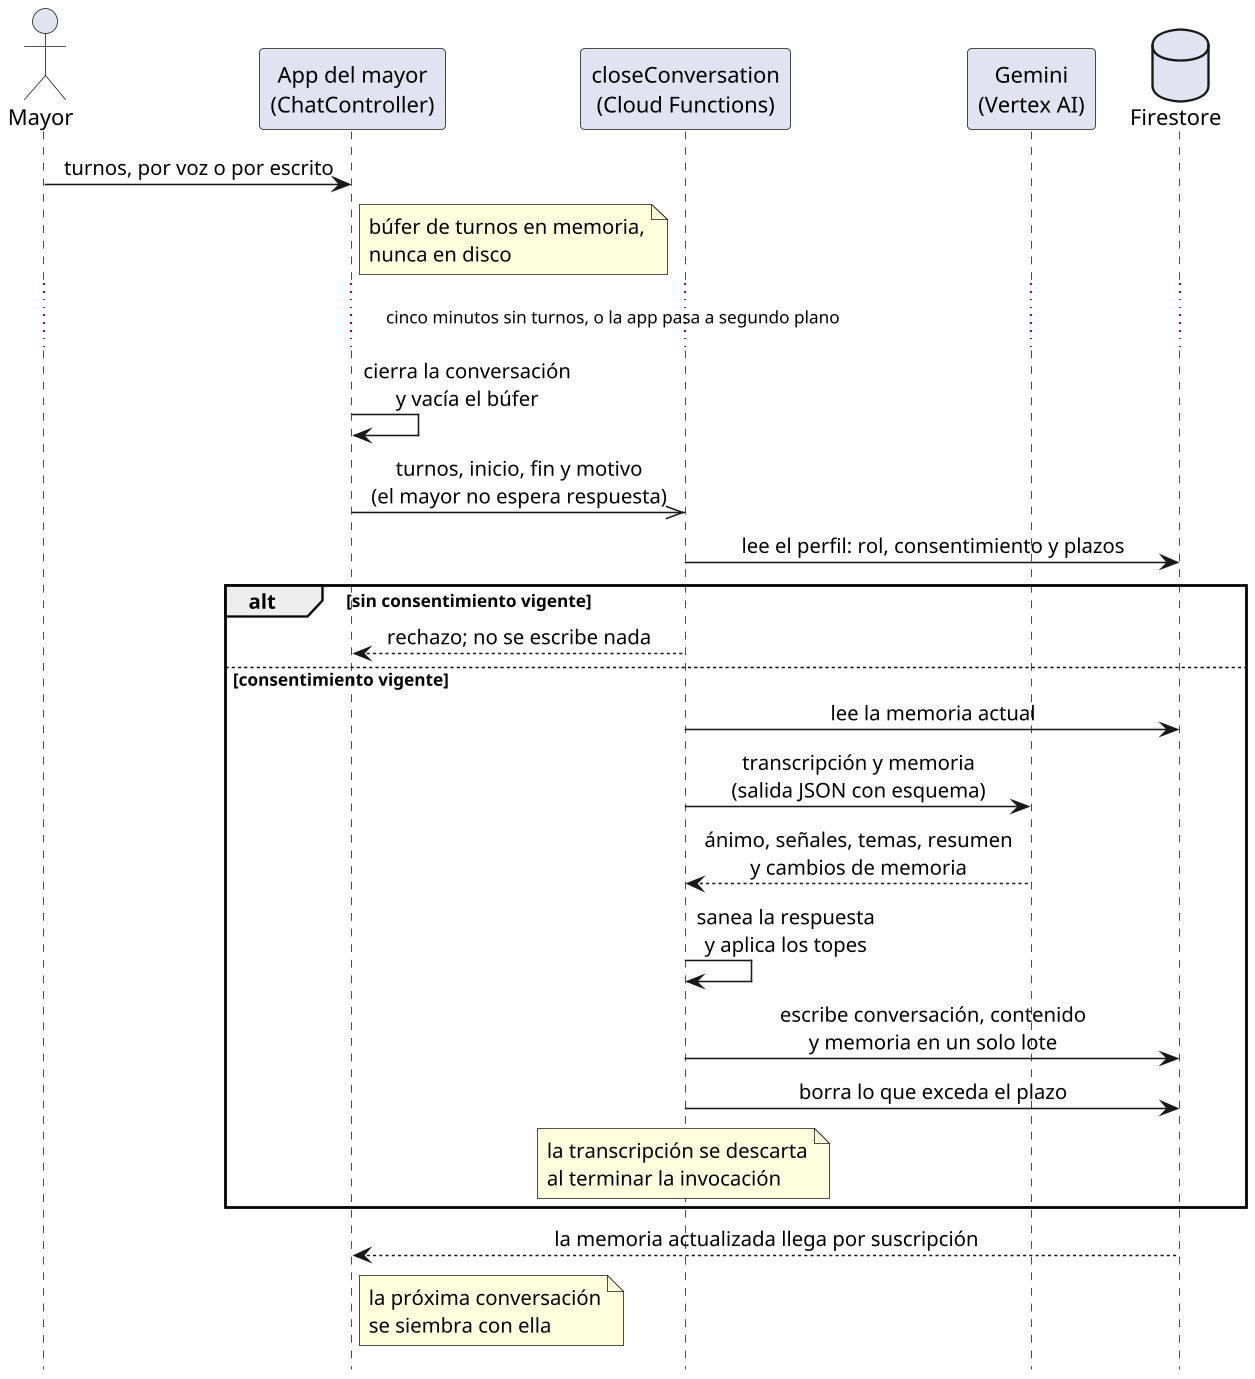
\includegraphics[width=0.85\textwidth]{imagenes/uml/secuencia_cierre.png}
    \caption{Cierre y análisis de una conversación: del búfer en memoria del teléfono a los documentos que se guardan, sin que la transcripción llegue a almacenarse.}
    \label{fig:secuencia-cierre}

    \vspace{2pt}
    {\footnotesize Fuente: Elaboración propia.}
\end{figure}

El análisis depende de los criterios del \emph{prompt}, que se versiona y queda registrado junto a cada resultado. El sentimiento es el del mayor y no el del diálogo, porque el asistente es cálido siempre y evaluar la conversación entera daría <<positivo>> casi siempre. Las clases son las tres de RF-8, sin escalas numéricas de valencia y activación que aparentarían una precisión que un modelo sin calibrar no tiene. Las señales salen de una lista cerrada de seis (soledad, tristeza, preocupación, malestar físico, desorientación y riesgo) y solo cuentan si las expresa el mayor, no si el asistente pregunta por ellas. El resumen ocupa una o dos frases en tercera persona, sin citas literales ni diagnósticos, y nombra a otras personas por su relación y no por su nombre. Y el \emph{prompt} advierte de que el texto procede de un reconocedor de voz, con sus errores. Si el modelo falla, la conversación se registra igualmente como actividad, con estado de fallo y sin reintentos, porque que el mayor hablase es un dato en sí mismo. El \autoref{lst:modelo-datos} muestra lo que se guarda, repartido en documentos que comparten identificador; el reparto lo impone el control de lo que ve el familiar, que se explica en el apartado~\ref{sec:privacidad}.

\begin{lstlisting}[style=Consola, caption={Lo que se guarda de cada conversación en Firestore. La transcripción no aparece en ninguno de los documentos.}, label={lst:modelo-datos}]
users/{elderId}/conversations/{id}         # "cómo me encuentro"
  startedAt, endedAt, elderTurns, endReason
  status:    analyzed | too_short | failed
  sentiment: positive | neutral | negative | null
  signals:   [loneliness, sadness, worry,
              physical_discomfort, confusion, risk]
  promptVersion, model, expireAt

users/{elderId}/conversationContents/{id}  # "de qué hablamos"
  endedAt, topics (máx. 5), summary, expireAt

users/{elderId}/memory/profile             # lo que recuerda
  facts (máx. 30), recent (3 últimos resúmenes), updatedAt
\end{lstlisting}

Las etiquetas de un modelo de lenguaje no están validadas clínicamente, de modo que se presentan como orientación y nunca como diagnóstico. Además, la señal de riesgo no convierte la aplicación en un sistema de alertas: el familiar la ve cuando abre el panel, y los avisos mediante notificaciones quedan como línea de trabajo futuro (apartado~\ref{sec:lineas-futuras}). La respuesta a una situación de crisis corresponde al chat en vivo, cuya instrucción de sistema incluye una regla explícita: responder con calma y sin quitarle importancia, animar a hablarlo con alguien de confianza y recordar el 024, la línea de atención a la conducta suicida, y el 112.

\subsection{La memoria del mayor}

Gemini no recuerda nada entre llamadas: el historial de la conversación es una lista de turnos en la memoria del teléfono, que el cliente reenvía entera a \code{chatTurn} en cada turno y que desaparece al terminar la conversación. Cualquier memoria entre conversaciones tiene que guardarse fuera y volver a entregarse al modelo. Se aprende al cerrar cada conversación, y no en vivo, porque solo se usa al empezar la siguiente. Aprenderla ahí es además gratis (no requiere otra llamada), porque la llamada del análisis ya lee la transcripción entera, y no añade latencia a lo único que el mayor percibe, la respuesta en vivo.

La misma llamada del cierre devuelve, por tanto, los cambios de la memoria y no un perfil reescrito: altas o correcciones por clave y claves que olvidar. Una lista de cambios explícitos se puede auditar, mientras que un perfil regenerado entero puede perder datos sin que nadie lo note. La función los aplica con topes estrictos, treinta datos en total y diez cambios por conversación con claves saneadas, y los guarda en un documento propio junto a los resúmenes de las tres últimas conversaciones. El \emph{prompt} excluye cualquier dato de salud, limita los datos de terceros a su nombre y su relación, y trata como borrado lo que el mayor pide olvidar.

Al empezar cada conversación, la sesión del modelo arranca con un bloque adicional en su instrucción de sistema, <<Lo que sabes de\ldots>> y <<De vuestras últimas conversaciones>>, acompañado de la indicación de usarlo con naturalidad, no recitarlo y no decir que se tienen notas; si la memoria está vacía, el bloque no aparece. La memoria llega al controlador del chat por suscripción y sin reconstruirlo, y una actualización nunca reinicia una conversación en curso: se aplica en la siguiente. Solo el nombre se aprende en vivo, mediante la función que el modelo invoca al oírlo, porque hace falta en la misma conversación. Es una forma ligera de generación aumentada por recuperación, sin infraestructura de búsqueda vectorial, que sería desproporcionada para treinta datos. La memoria va, por tanto, una conversación por detrás: lo que el mayor cuenta en una conversación se recuerda a partir de la siguiente.

\subsection{El seguimiento del bienestar: el panel del familiar y <<Mi semana>>}
\label{sec:bienestar}

El análisis tiene dos destinatarios: el familiar y el propio mayor. Si solo lo viera el familiar, al mayor independiente no le aportaría nada y al vinculado lo dejaría como objeto de seguimiento y no como destinatario de lo que se dice de él. Los dos ven los mismos datos en pantallas distintas, sin coste de arquitectura. Los modelos de lectura del análisis y la agregación semanal viven en \code{core/}, y la agregación es una función pura con pruebas, \code{summarizeWeek}, que calcula los días con conversación, el ánimo predominante, los temas más repetidos, los temas de las conversaciones con preocupación y el recuento de señales. Si cada pantalla calculara por su cuenta, el mayor y su familiar acabarían viendo números distintos. Lo que cambia entre ambas es la presentación.

El \textbf{panel del familiar} ordena sus secciones por fiabilidad: primero la actividad, que no depende de ningún modelo (cuándo habló por última vez, cuántos días y cuánto tiempo), y después las señales, el ánimo, los temas, la lista de conversaciones con su detalle y lo que el asistente recuerda. Todo lo que estima el modelo lleva el aviso <<Orientativo: lo estima un modelo de IA a partir de lo que dice. No es un diagnóstico>>. Si alguna conversación de la semana registró la señal de riesgo, el panel lo indica arriba y en rojo, con el 112 y el 024, que atiende también a familiares. Y si el mayor ha restringido lo que comparte, el panel lo explica en lugar de mostrar un error de permisos.

\textbf{<<Mi semana>>}, la pantalla del mayor, cuenta la semana con frases y no con gráficas, en segunda persona y en tono de refuerzo, con un botón <<Escuchar>> que las lee en voz alta (<<Esta semana hemos hablado 4 días>>, <<La mayoría de las veces te he notado bien>>). Una fila de siete días marca cuándo se habló y no cómo se encontraba cada día, porque busca reforzar y no evaluar. Las señales de soledad, tristeza o riesgo no se nombran nunca; de ellas solo aparece, suavizado, <<lo que más te ha rondado la cabeza>>. En caso de empate entre ánimos la agregación devuelve neutro: ante la duda, no se afirma ni que estuvo bien ni que estuvo mal. La pantalla indica, por último, qué parte de su análisis ve su familiar, con acceso directo para cambiarlo, así que <<Mi semana>> también le muestra lo que se guarda de él. El acceso aparece en la pantalla principal para todo mayor con el consentimiento activo y al menos una conversación analizada, sea independiente o vinculado. Las dos pantallas se recogen en el manual de usuario del apéndice~\ref{ap:manual}.

\section{Privacidad desde el diseño: el consentimiento informado}
\label{sec:privacidad}

De todo lo que hace el sistema, analizar las conversaciones de una persona mayor es lo más delicado, y es también lo que más lo separa de los compañeros conversacionales revisados en el capítulo~\ref{cap:marco-teorico}, uno de los cuales fue sancionado precisamente por carecer de base jurídica para tratar datos. Inferir el estado de ánimo o registrar molestias físicas puede revelar datos relativos a la salud, una categoría especial cuyo tratamiento el RGPD prohíbe salvo excepciones (art.~9.1), y la única realista para esta aplicación es el consentimiento explícito del interesado (art.~9.2.a) \citep{RGPD2016}. Este apartado explica cómo se ha diseñado ese consentimiento, cómo se hace cumplir y cómo se gobierna el plazo de conservación. Es un diseño conforme a los principios del Reglamento, no un dictamen jurídico.

\subsection{Quién consiente, cuándo y cómo}

El Reglamento define el consentimiento como una manifestación de voluntad libre, específica, informada e inequívoca, mediante una declaración o una clara acción afirmativa (art.~4.11), y precisa que el silencio, las casillas ya marcadas o la inacción no lo constituyen (considerando~32). Hace falta, por tanto, un gesto, y el diseño solo decide cuál. Para esta población es una pantalla propia con una sola pregunta, <<¿Quieres que guarde un resumen de nuestras conversaciones?>>, y dos botones del mismo tamaño, <<Sí, quiero>> y <<Ahora no>>, de modo que negarse cuesta exactamente lo mismo que aceptar. No es una casilla, porque una casilla de tamaño convencional incumpliría el área táctil mínima de RNF-2. Un botón <<Escuchar>> lee en voz alta la pregunta y su explicación, y <<Saber más>> abre la versión completa del texto.

Consiente siempre el mayor, en su propio dispositivo, también cuando está vinculado. Que consintiera el familiar no sería válido ni deseable porque, en esta aplicación, <<vinculado>> significa que al mayor le ayudan con la tecnología, no que exista una medida de apoyo que convierta al familiar en su representante, que sería paternalista. El familiar \textbf{ayuda a decidir}, el mayor \textbf{decide}. La pregunta aparece una sola vez y en el momento más temprano posible: justo después de elegir el modo independiente o justo después de completarse la vinculación, un momento que suele ser presencial, porque el familiar lee el código en la pantalla del mayor y puede explicarle la pregunta en persona. Se implementa como un paso del enrutador, y <<Ahora no>> también se registra, para no volver a preguntar.

El texto está en lenguaje llano y se ofrece en dos capas, una breve en la pregunta y otra completa en <<Saber más>>, en la línea de los artículos~12 y~13. Explica por separado qué se guarda (un resumen breve de cada conversación y cómo se ha sentido, nunca lo que dice palabra por palabra), qué se recuerda (lo que cuenta de su familia o de sus gustos, nunca nada de su salud), cómo se hace (lo hablado se envía a los servidores de Google, que lo analizan y no lo guardan), quién lo ve (su familiar, por su nombre, o solo él), cuánto tiempo se conserva y cómo puede retirarlo. El texto está versionado, y la versión leída se registra con la respuesta. Un único consentimiento cubre el análisis y la memoria, porque ambos sirven al propio mayor. Si está vinculado, la pregunta le dice además que su familiar verá cómo se encuentra y un resumen de lo que hablan, y el <<sí>> incluye ese nivel, que puede cambiar después en Ajustes. Y nada se trata hasta el <<sí>>: el consentimiento está desactivado por defecto, que es la protección de datos por defecto del artículo~25.2.

\subsection{Cómo se hace cumplir}

Un consentimiento que solo respeta la interfaz no protege nada, porque el familiar tiene sesión propia y podría leer cuanto las reglas le permitan, con esta aplicación o con otra. Por eso las tres garantías centrales se imponen en el servidor.

La primera es la prueba del consentimiento. El responsable debe poder demostrar que el interesado consintió (art.~7.1), y una hora tomada del dispositivo no demuestra nada. El registro del consentimiento, con la respuesta, la hora y la versión del texto leído, solo lo escribe \code{setConversationConsent}, con la hora del servidor; las reglas impiden que lo escriba cualquier cliente, incluido el propio mayor, y que un documento nazca con un consentimiento de serie. La función toma además la identidad de la sesión, de modo que un familiar no puede consentir por su mayor ni siquiera llamándola directamente.

La segunda es que sin consentimiento no se analiza nada. El cliente no envía la conversación si no lo hay, pero la garantía real es que \code{closeConversation} lo vuelve a comprobar y, si no está vigente, rechaza la petición sin escribir nada.

La tercera es qué ve el familiar. Hay tres niveles con nombre: <<Nada>>; <<Cómo me encuentro>>, que incluye la actividad, el ánimo y las señales; y <<Cómo me encuentro y de qué hablamos>>, que añade los temas, los resúmenes y la memoria. El <<sí>> del mayor vinculado fija el tercero, salvo que antes hubiera elegido otro, y a partir de ahí solo el mayor puede cambiarlo. Hacerlo cumplir tropieza con una limitación de Firestore, la de que las reglas no pueden filtrar campos, porque leer un documento es leerlo entero. Por eso cada conversación se reparte en dos documentos, y las reglas conceden la lectura de cada colección según el nivel. El \autoref{lst:reglas} muestra la función que lo decide.

\begin{lstlisting}[float=tbp, caption={Regla de lectura del familiar sobre el análisis del mayor (extracto de \texttt{firestore.rules}).}, label={lst:reglas}]
function companionMayRead(elderId, levels) {
  let elder = get(/databases/$(database)/documents/users/$(elderId)).data;
  return isSignedIn()
    && elder.get('linkedCompanionId', null) == request.auth.uid
    && elder.get('conversationConsent', {}).get('granted', false) == true
    && elder.get('companionSharing', 'none') in levels;
}

match /users/{userId} {
  match /conversations/{id} {             // cómo me encuentro
    allow read: if isOwner(userId)
      || companionMayRead(userId, ['wellbeing', 'full']);
    allow write: if false;                // solo el servidor
  }
  match /conversationContents/{id} {      // de qué hablamos
    allow read: if isOwner(userId)
      || companionMayRead(userId, ['full']);
    allow write: if false;
  }
}
\end{lstlisting}

La condición se evalúa al leer y no se copia al escribir: al bajar el nivel se oculta al instante también todo el historial. Las pruebas contra el emulador lo comprueban: un familiar con nivel <<Cómo me encuentro>> que intenta leer los resúmenes es rechazado, y uno cuyo mayor ha retirado el consentimiento no lee nada, aunque el nivel fuera el completo. Las señales, también la de riesgo, pertenecen al nivel intermedio, así que si el mayor elige <<Nada>> su familiar no sabrá que la hubo. Prima la autonomía del mayor, coherente con que la aplicación no es un sistema de alertas.

\subsection{Retirada, plazos y borrado}

Retirar el consentimiento debe ser tan fácil como darlo (art.~7.3). En Ajustes, la fila <<Guardar mis conversaciones>>, dentro de <<Mis conversaciones>>, permite hacerlo con un toque y una confirmación que muestra la fecha en que se borrará lo guardado. La retirada tiene efecto inmediato sobre el tratamiento: se detiene el análisis, la memoria deja de inyectarse y el familiar pierde el acceso, porque sus reglas de lectura exigen el consentimiento vigente además del nivel. Lo ya guardado, en cambio, no se borra al instante. Queda congelado durante un periodo de gracia igual a la mitad del plazo de conservación vigente, cuarenta y cinco días con el plazo por omisión, durante el que nadie lo trata ni lo lee salvo el propio mayor; si vuelve a consentir antes, lo recupera, y si no, se borra. Así, un toque equivocado, fácil en esta población, no le cuesta al mayor meses de historia. Esto choca con el artículo~17.1.b, que pide suprimir los datos sin dilación indebida cuando se retira el consentimiento. Se justifica por su finalidad y porque durante el periodo los datos no se tratan.

El borrado no exige ninguna tarea programada. Cada documento del análisis lleva una fecha de caducidad, y una política de caducidad (TTL) de Firestore lo elimina al vencer, normalmente dentro de las veinticuatro horas siguientes \citep{FirestoreTTL}. Al retirar el consentimiento, la función adelanta esa fecha en cada documento a la más temprana entre su caducidad normal y el final del periodo de gracia, de modo que retirarlo nunca alarga la vida de un dato; al volver a consentir, la restaura.

Los plazos, por último, son configurables: el tiempo sin turnos que cierra una conversación (2, 5, 10 o 15~minutos) y el plazo de conservación (30, 60, 90 o 180~días, con 90 por omisión). Siguen el reparto de la revelación progresiva: los fija el propio mayor si es independiente y su familiar, desde el panel, si está vinculado. Como el segundo afecta a datos personales, el servidor lo acota entre 30 y 180~días diga lo que diga el documento, y en cada cierre borra lo que haya quedado fuera del plazo vigente, de modo que acortarlo borra de verdad sin esperar a la caducidad de lo antiguo. El mayor vinculado consiente con el plazo vigente en ese momento y su familiar puede alargarlo después hasta seis meses; el texto del consentimiento lo advierte y la pantalla de detalle muestra siempre el valor actual.

\subsection{Correspondencia con el RGPD y límites}

La \autoref{tab:rgpd} resume cómo se realizan en el sistema las obligaciones del Reglamento que afectan al tratamiento de las conversaciones.

\begin{table}[!tb]
    \centering
    \caption{Correspondencia entre las obligaciones del RGPD y su realización en el sistema.}
    \label{tab:rgpd}
    \small
    \begin{tabularx}{\textwidth}{@{}>{\RaggedRight\arraybackslash}p{0.36\textwidth} >{\RaggedRight\arraybackslash}X@{}}
        \toprule
        \textbf{Obligación del RGPD} & \textbf{Realización en Quiet Companion} \\
        \midrule
        Base de licitud para datos de salud: consentimiento explícito (arts.~6.1.a y 9.2.a) & Pantalla propia con un gesto afirmativo del mayor; el familiar no puede consentir por él \\
        Consentimiento inequívoco (art.~4.11, considerando~32) & Dos botones del mismo tamaño; ni silencio ni casillas premarcadas \\
        Información clara y accesible (arts.~12 y 13) & Texto llano y versionado, en dos capas y con lectura en voz alta \\
        Demostrar el consentimiento (art.~7.1) & Registro escrito solo por el servidor, con su hora y la versión del texto \\
        Retirarlo tan fácilmente como se dio (art.~7.3) & Una fila en Ajustes, un toque y una confirmación \\
        \raggedright Minimización de datos (art.~5.1.c) & La transcripción no se almacena; sin texto por debajo de tres turnos; un solo análisis \\
        Limitación del plazo de conservación (art.~5.1.e) & Caducidad automática (TTL); plazo de 30 a 180~días acotado por el servidor \\
        Protección de datos desde el diseño y por defecto (art.~25) & Desactivado por defecto; niveles de compartición impuestos por las reglas \\
        Derecho de acceso (art.~15) & <<Mi semana>> muestra al mayor lo que se guarda de él y quién lo ve \\
        \raggedright Derecho de supresión (art.~17.1.b) & Borrado al final del periodo de gracia tras la retirada \\
        Seguridad del tratamiento (art.~32) & Reglas verificadas contra el emulador; registros sin texto de las conversaciones \\
        \bottomrule
    \end{tabularx}

    \vspace{2pt}
    {\footnotesize Fuente: Elaboración propia a partir del Reglamento (UE) 2016/679.}
\end{table}

Un despliegue real con personas mayores y datos de salud exigiría una evaluación de impacto relativa a la protección de datos (art.~35), que queda como trabajo futuro. Y lo hablado sale del dispositivo hacia Google en dos momentos: en cada turno de la conversación en vivo y en su análisis al cierre. En ninguno de los dos puede el proveedor usarlo para mejorar sus modelos: los dos se sirven desde Vertex AI en una región europea, cuyas condiciones excluyen entrenar con los datos del cliente sin su permiso \citep{VertexDataGovernance}. El texto del consentimiento advierte de ese tratamiento por un tercero.

\section{Conversación por escrito}
\label{sec:teclado}

La voz es el canal principal del mayor, pero no siempre el adecuado: en una sala de espera, de noche con alguien durmiendo, con ronquera o con una dificultad del habla, o simplemente cuando el reconocedor no le entiende. Para esos casos, HU-8 añade la conversación por escrito, a un toque del botón <<¿Teclado?>> de la pantalla principal.

El canal apenas afecta a la arquitectura, porque esta separa la entrada de la conversación: el método del controlador que envía un turno no sabe de dónde viene el texto. Un turno escrito sigue por tanto el mismo camino que uno hablado, con la misma sesión del modelo, el mismo búfer en memoria y la misma frontera de conversación, así que cuenta para el mínimo de tres turnos y llega al análisis al cierre sin tocar el servidor. No lleva marca de canal, porque el análisis trata de lo que dice el mayor y no de cómo lo dice.

La respuesta a un turno escrito se muestra sin leerse, salvo que el mayor lo pida, porque el motivo más común para escribir es estar donde no se quiere que el teléfono hable, y un botón <<Escuchar>>, que mientras suena pasa a <<Parar>>, devuelve la voz a quien escribe por una dificultad del habla pero necesita oír la respuesta. El turno hablado no cambia. Pulsar <<¿Teclado?>> sustituye el micrófono por un campo de texto, con la letra escalada por la preferencia del mayor, y un botón <<Enviar>> de $80\times80$ píxeles lógicos; el campo toma el foco al aparecer, de modo que el teclado del sistema se abre sin otro toque, y se cierra al tocar fuera del campo o con un botón propio, para dejar ver la respuesta entera. El mismo botón pasa a decir <<¿Hablar?>> para volver. Si el envío falla, el texto vuelve al campo para no obligar a escribirlo de nuevo.

El modo vive en el estado del controlador y no en el \emph{widget}, de modo que sobrevive a ir a Ajustes o a Emergencia y volver, y el controlador puede actuar al cambiarlo: pasar al teclado con el micrófono abierto descarta lo que se estaba oyendo en lugar de enviar un texto que el mayor no ha confirmado. Y como una voz cortada termina tarde, cuando ya ha empezado otra cosa, cada turno, escucha o lectura toma un número de orden, y la vuelta a reposo tras hablar solo se aplica si lo que la lanzó sigue siendo lo último. Sin ese control, una respuesta cortada por un turno escrito devolvería la pantalla a reposo con el turno nuevo en curso y permitiría enviar un segundo mensaje simultáneo a la misma sesión del modelo. El predicado que decide si se admite un turno escrito está en un solo sitio, el estado del chat, y lo consultan por igual la pantalla y el controlador.

\section{Cronología del desarrollo}
\label{sec:cronologia}

El plan de hitos se documenta en el capítulo~\ref{cap:metodologia}; lo que sigue es cómo se construyó, fase a fase. La \autoref{tab:fases} resume las fases y su correspondencia con los hitos del plan.

\begin{table}[htbp]
    \centering
    \caption{Fases del desarrollo y su correspondencia con los hitos (2026).}
    \label{tab:fases}
    \small
    \begin{tabularx}{\textwidth}{@{}>{\RaggedRight\arraybackslash}p{0.27\textwidth} l l >{\RaggedRight\arraybackslash}X@{}}
        \toprule
        \textbf{Fase} & \textbf{Periodo} & \textbf{Hitos} & \textbf{Qué entregó} \\
        \midrule
        0. Arranque                        & Marzo      & ---    & Repositorio y descripción del proyecto \\
        1. Prototipo y \emph{stack}        & Marzo      & M1, M2 & Voz de extremo a extremo y elección del \emph{stack} \\
        2. Onboarding y panel remoto       & Abril      & M1, M3 & Onboarding dual, emparejamiento y panel del familiar \\
        3. Estabilización                  & Mayo--jul. & M4     & Navegación, inyección de dependencias, emergencia, ajustes y primera suite de pruebas \\
        4. Voz en la nube y seguridad      & Jul.--sep. & M5     & Voz Chirp~3:~HD, escucha por turnos, reglas verificadas y vinculación en el servidor \\
        5. Privacidad y bienestar          & Septiembre & M6, M7 & Consentimiento, análisis al cierre, memoria, panel y <<Mi semana>> \\
        6. Conversación por escrito        & Octubre    & M8     & Modo teclado, pausa de escucha configurable y elección de voz \\
        \bottomrule
    \end{tabularx}

\end{table}

El proyecto arrancó demostrando lo más arriesgado primero, que la cadena de reconocimiento, generación y síntesis de voz funcionaba de extremo a extremo, antes de construir nada a su alrededor. Con la fase~4, la aplicación dejó de ser un cliente que habla con servicios ajenos y pasó a tener servidor propio, primero para la voz y después para la seguridad. En la fase~5, el consentimiento precedió a cualquier análisis, porque ningún dato de una conversación podía tratarse antes de que existiera el permiso que lo autoriza. La cadencia no fue uniforme, por las razones expuestas en el capítulo~\ref{cap:metodologia}, pero cada fase cerró un incremento coherente y dejó el código compilable y con sus pruebas en verde.

\section{Cierre del capítulo}

El sistema descrito en este capítulo cumple los requisitos comprometidos.

En cuanto a la verificación, el árbol de código pasa el análisis estático sin advertencias (RNF-13) y cuenta con ochenta y seis casos de prueba en tres suites complementarias: cincuenta y uno en Dart, que cubren los modelos, el enrutador, la entrada del mayor y su cuenta, los controladores del chat y del panel, la escucha por turnos, las pantallas del mayor, la agregación semanal y la síntesis de voz; doce de reglas de seguridad contra el emulador de Firestore; y veintitrés sobre la lógica pura de las funciones del servidor. A ellas se suma la prueba en dispositivo, la única que comprueba las suposiciones sobre el comportamiento del reconocedor de voz y del reproductor de audio. Todas las historias, de HU-1 a HU-8, se han recorrido de principio a fin en un teléfono Android.

En conjunto, la aplicación conversa por voz o por escrito, recuerda lo que el mayor le cuenta, informa de cómo se encuentra a quien él autoriza, se configura en remoto, llama a emergencias y se adapta a las capacidades de quien la usa, sin guardar nunca lo que dice palabra por palabra. Lo que queda fuera de ese alcance se recoge en el \autoref{cap:desarrollo-futuro}.


\chapter{Conclusiones y trabajo futuro}
\label{cap:desarrollo-futuro}

\section{Conclusiones}
\label{sec:conclusiones}

El objetivo general del trabajo era desarrollar un prototipo funcional de aplicación móvil que acompañe por voz a personas mayores en situación de soledad no deseada y que resulte accesible para ese perfil de usuario. El prototipo existe y cumple los objetivos específicos comprometidos; la tabla~\ref{tab:cumplimiento-oe} recoge, para cada uno, dónde se documenta la evidencia.

\begin{table}[htbp]
    \centering
    \caption{Cumplimiento de los objetivos específicos y apartado donde se documenta.}
    \label{tab:cumplimiento-oe}
    \small
    \begin{tabularx}{\textwidth}{@{}l >{\RaggedRight\arraybackslash}X@{}}
        \toprule
        \textbf{Objetivo} & \textbf{Evidencia} \\
        \midrule
        OE-1 & Onboarding dual con revelación progresiva y vinculación atómica ejecutada en el servidor (apartado~\ref{sec:seguridad}). \\
        \addlinespace
        OE-2 & Ciclo completo de voz con respaldo al motor del dispositivo, y conversación por escrito como vía alternativa (apartado~\ref{sec:teclado}). \\
        \addlinespace
        OE-3 & Pisos tipográficos, áreas táctiles de al menos $80\times80$~px, pulsación simple y una paleta que supera los umbrales de contraste de WCAG~2.2 en toda la interfaz del mayor (apartado~\ref{sec:color}). \\
        \addlinespace
        OE-4 & Configuración local y remota, propagada en tiempo real en ambas direcciones (apartado~\ref{sec:ssot}). \\
        \addlinespace
        OE-5 & Memoria, análisis al cierre, panel de bienestar y «Mi semana» bajo consentimiento del propio mayor, sin almacenar la transcripción (apartados~\ref{sec:conversacion} y~\ref{sec:privacidad}); cubiertos por pruebas automáticas y verificados en dispositivo. \\
        \addlinespace
        OE-6 & Arquitectura Clean Feature-Sliced sin acoplamiento horizontal (apartado~\ref{sec:arquitectura}) y gestión Kanban (apartado~\ref{sec:tablero}). \\
        \bottomrule
    \end{tabularx}

\end{table}

Más allá del balance por objetivos, el desarrollo deja tres conclusiones que trascienden a este proyecto concreto.

La primera es que la accesibilidad funciona mejor como restricción de diseño que como capa de acabado. Las decisiones más reconocibles de la aplicación no se tomaron para cumplir una norma después de diseñar, sino que se derivaron de ella: un único control grande en la pantalla principal, escalas con nombre en lugar de deslizadores, un consentimiento recogido con dos botones del mismo tamaño y no con una casilla, y una semana contada con frases y no con gráficas. Centralizar esas reglas en el sistema de diseño hizo además que cada pantalla nueva las heredara sin esfuerzo adicional.

La segunda es que la privacidad solo es una propiedad del sistema cuando la hace cumplir el servidor. Lo que el mayor decide que ve su familiar no depende de que la aplicación del familiar se comporte bien, sino de unas reglas verificadas contra el emulador y de un reparto del almacenamiento pensado para que esas reglas puedan aplicarse; y la transcripción no se protege prometiendo no mirarla, sino no guardándola nunca. La plataforma de funciones gestionadas fue la que hizo viable ese planteamiento para un único desarrollador: permitió tener lógica de servidor de confianza sin operar servidor alguno.

La tercera es metodológica: la verificación necesita varios niveles, y ninguno sustituye a los otros. Las pruebas de la lógica protegen de los errores propios; las de las reglas contra el emulador comprueban que el sistema niega lo que no debe permitir, algo que ninguna prueba de la aplicación puede ver; y solo el dispositivo confirma las suposiciones sobre lo que el proyecto no controla, como el momento en que el reconocedor de voz entrega su último resultado. Probar cada pieza en el nivel que le corresponde es lo que permite defender el resto de afirmaciones de esta memoria.

Queda, por último, la premisa con la que se planteó el trabajo: la tecnología debe complementar el vínculo humano y no sustituirlo. El resultado la respeta en su diseño, porque el familiar forma parte del circuito y es el mayor quien decide qué sabe de él, pero no puede afirmar que la herramienta reduzca la soledad de nadie. Esa pregunta, que es la que de verdad importa, es la primera de las líneas que siguen.

\section{Líneas de trabajo futuro}
\label{sec:lineas-futuras}

Las ocho Historias de Usuario del catálogo están implementadas, y las líneas que siguen quedan fuera de él. Se ordenan de mayor a menor alcance, que no coincide con el orden de dificultad técnica.

La limitación más relevante del trabajo, señalada ya en el capítulo~\ref{cap:marco-teorico}, es la \textbf{ausencia de validación con usuarios reales}. Un estudio de campo con personas mayores, con instrumentos validados como la Escala de Soledad de De Jong Gierveld \citep{DeJongGierveld2010}, permitiría contrastar si la herramienta produce algún efecto medible sobre la dimensión social de la soledad, que es la única que la propuesta aspira a abordar. Ese estudio permitiría además contrastar las etiquetas del análisis emocional con la percepción del propio mayor y de su familiar, que el sistema presenta solo como orientación.

La segunda es de protección de datos, y es condición para cualquier despliegue fuera del ámbito académico: una \textbf{evaluación de impacto relativa a la protección de datos} (art.~35 del RGPD), obligada en un tratamiento de datos de salud de personas vulnerables. Junto a ella, tres mejoras en el diseño del consentimiento: una opción «Borrarlo ya» que suprima de inmediato lo guardado al retirarlo, y resuelva así la tensión con el artículo~17; la posibilidad de que el familiar \emph{solicite} el consentimiento a distancia para que el mayor lo confirme en su propio dispositivo; y la corrección de la memoria, porque un dato mal transcrito («Paulo» por «Pablo») solo se corrige si el mayor lo aclara en una conversación posterior.

En el terreno funcional quedan dos extensiones de alcance acotado. La primera es un \textbf{sistema de notificaciones \textit{push}} al familiar. El familiar solo conoce la señal de riesgo al abrir el panel (apartado~\ref{sec:conversacion}), y el valor de un seguimiento reside justamente en no tener que consultarlo. Firebase Cloud Messaging encaja de forma natural en una arquitectura construida sobre Firebase: la misma función que analiza la conversación al cerrarse podría avisar al dispositivo del familiar. El aviso tendría que obedecer el nivel de compartición elegido por el mayor, de modo que nadie reciba por notificación lo que no podría leer en el panel, y limitarse a invitar a abrirlo, sin mostrar en la pantalla de bloqueo nada de lo hablado. Ni siquiera así la aplicación se convertiría en un sistema de emergencias, porque una notificación no garantiza que alguien la atienda a tiempo.

La segunda es admitir \textbf{varios familiares por mayor} a la vez que \textbf{varios mayores por familiar}, ampliando a $0..*$ la cardinalidad que el modelo conceptual del capítulo~\ref{cap:analisis} fija en $0..1$. Esa restricción simplifica el modelo, pero no cubre los casos frecuentes de varios hijos que se reparten el cuidado, o la existencia de varias personas de edad avanzada en la familia o entorno cercano. Ampliarla obligaría a decidir si cada uno ve lo mismo.

Por último, dos líneas de naturaleza técnica. La evolución hacia una \textbf{conversación de audio nativa}, sustituyendo la cadena de transcripción, generación y síntesis por un modelo multimodal que reciba y devuelva voz, atacaría directamente la latencia percibida que fija RNF-7 y eliminaría la pérdida de matiz que supone convertir el habla en texto antes de interpretarla, aunque obligaría a revisar el modelo de privacidad, porque el análisis dejaría de trabajar sobre texto. Y una \textbf{integración continua} que ejecute de forma automática las tres suites de pruebas en cada cambio, sin la cual la cobertura conseguida se degrada con el tiempo sin que nadie lo advierta.


%%% --- Permite partir las URL largas de la bibliografia para que no invadan el margen --- %%%
\setcounter{biburlnumpenalty}{9000}
\setcounter{biburllcpenalty}{9000}
\setcounter{biburlucpenalty}{9000}
\setlength{\emergencystretch}{3em}
% Solo lo citado (APA).
\printbibliography[
title={Bibliografía},
heading=bibintoc]
%\bibliography{bibliografia/bibliografia}\addcontentsline{toc}{chapter}{Bibliografía}
%\bibliographystyle{unsrt}


%
\appendix
% Apéndice: manual de usuario.
% Capturas en imagenes/manual/, recortadas sin barra de estado ni barra de navegación (945 x 1871 px).

\chapter{Manual de usuario}
\label{ap:manual}

\captionsetup[sub]{font=scriptsize}

\newcommand{\manualhueco}{\hspace{0.02\textwidth}}

Quiet Companion se usa desde dos móviles. En el de la persona mayor está el asistente con el que conversa; en el de un familiar, si ella lo desea, un panel desde el que la acompaña a distancia. Este manual explica cada parte por separado: la sección~\ref{sec:manual-mayor} está pensada para la persona mayor o para quien la ayude a empezar, y la sección~\ref{sec:manual-familiar}, para el familiar. La aplicación necesita un móvil Android 7.0 o posterior con conexión a Internet.

\section{La persona mayor}
\label{sec:manual-mayor}

\subsection{Primeros pasos}

\begin{figure}[!htb]\centering
  \begin{subfigure}[t]{0.165\textwidth}\centering
    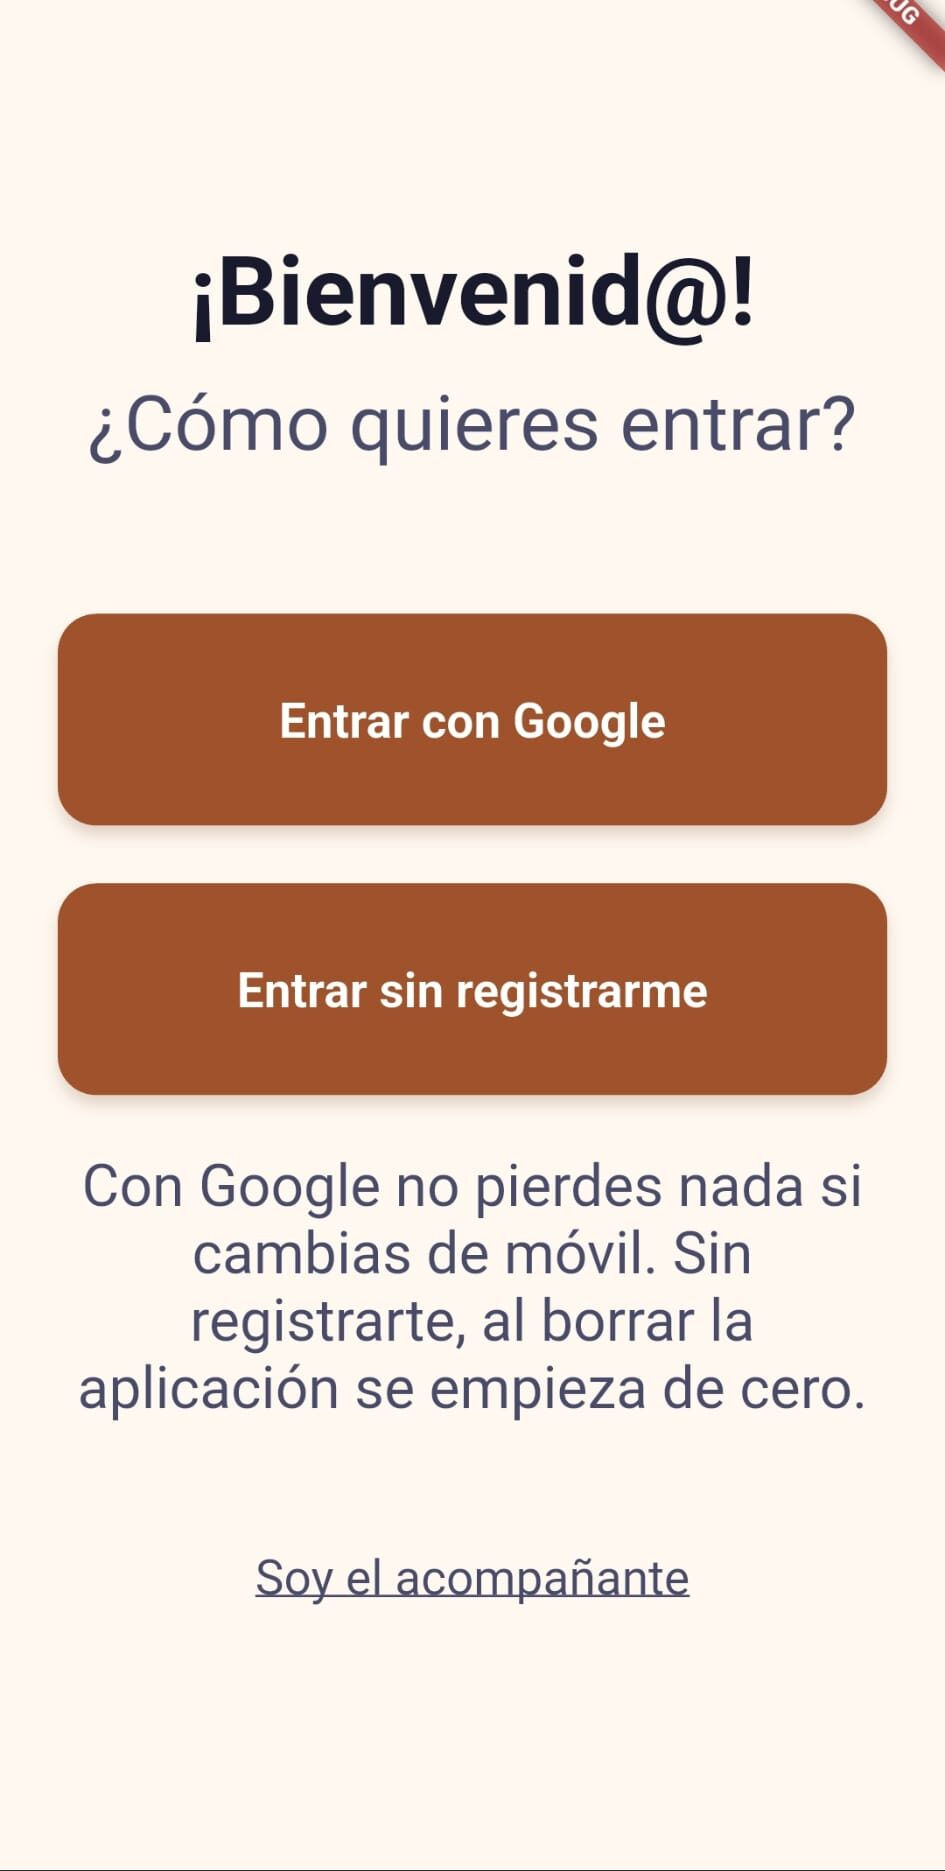
\includegraphics[width=\linewidth]{imagenes/manual/mayor-entrar}
    \caption{Entrar}
  \end{subfigure}\manualhueco
  \begin{subfigure}[t]{0.165\textwidth}\centering
    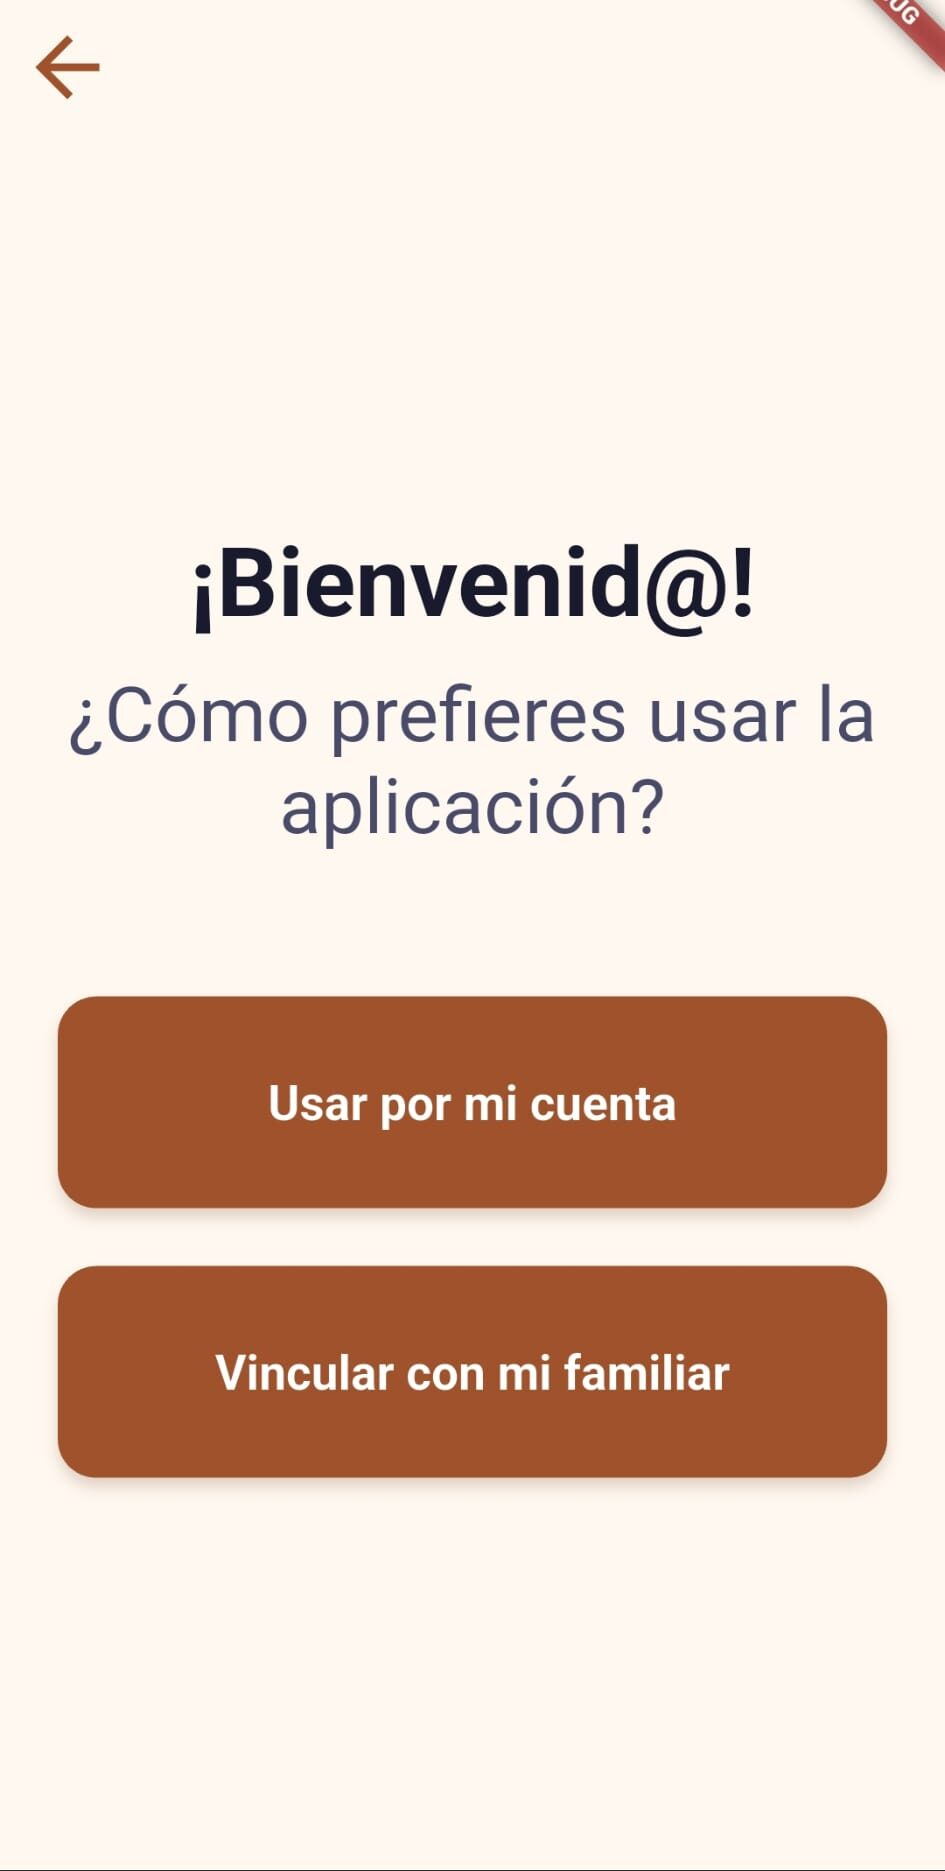
\includegraphics[width=\linewidth]{imagenes/manual/mayor-modo}
    \caption{Modo de uso}
  \end{subfigure}\manualhueco
  \begin{subfigure}[t]{0.165\textwidth}\centering
    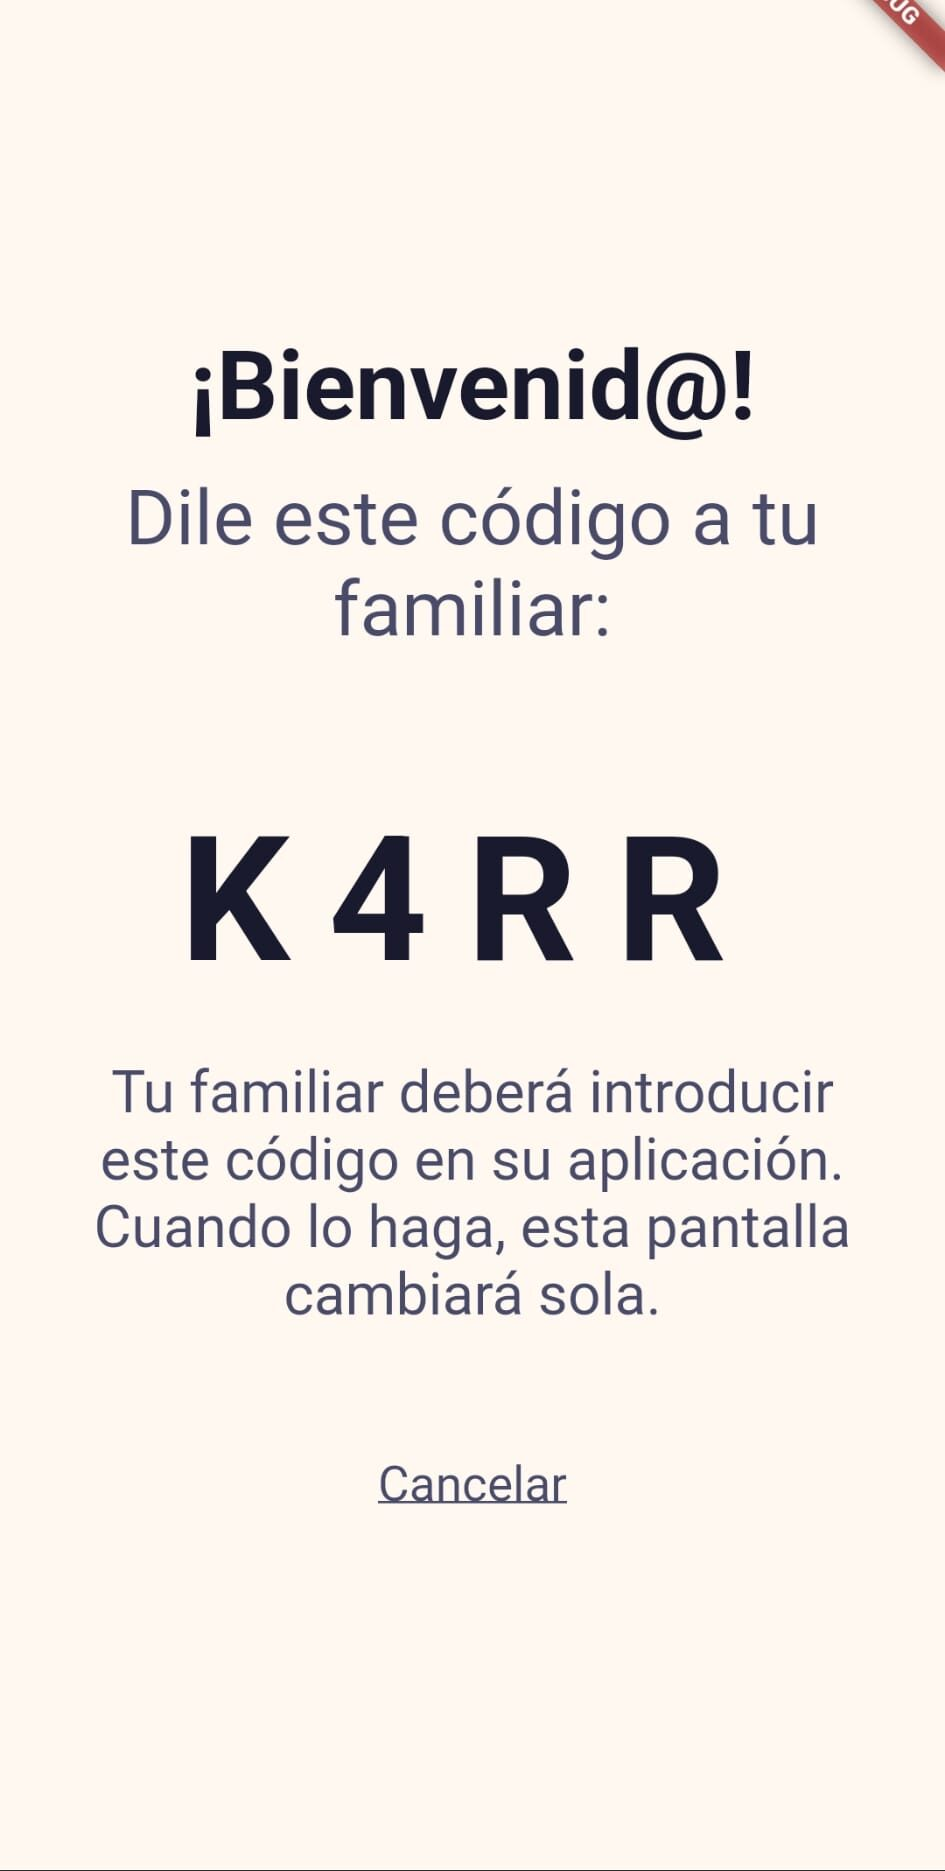
\includegraphics[width=\linewidth]{imagenes/manual/mayor-codigo}
    \caption{Código}
  \end{subfigure}\manualhueco
  \begin{subfigure}[t]{0.165\textwidth}\centering
    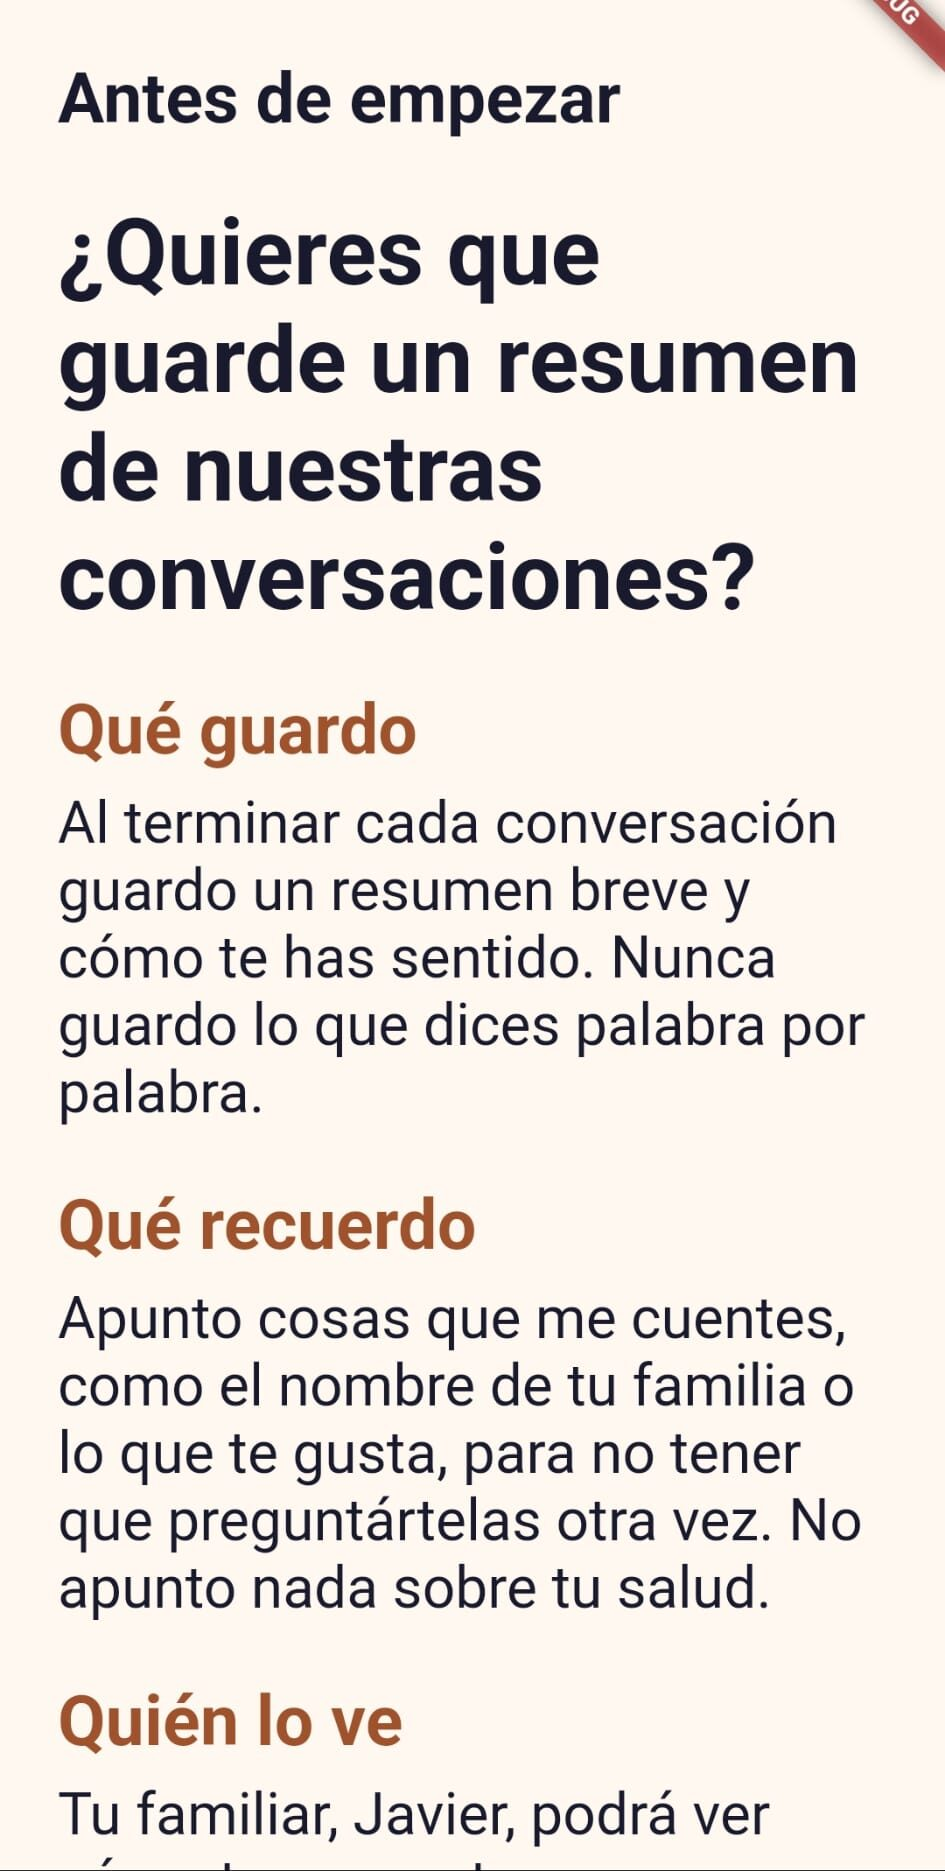
\includegraphics[width=\linewidth]{imagenes/manual/mayor-consentimiento}
    \caption{Pregunta}
  \end{subfigure}\manualhueco
  \begin{subfigure}[t]{0.165\textwidth}\centering
    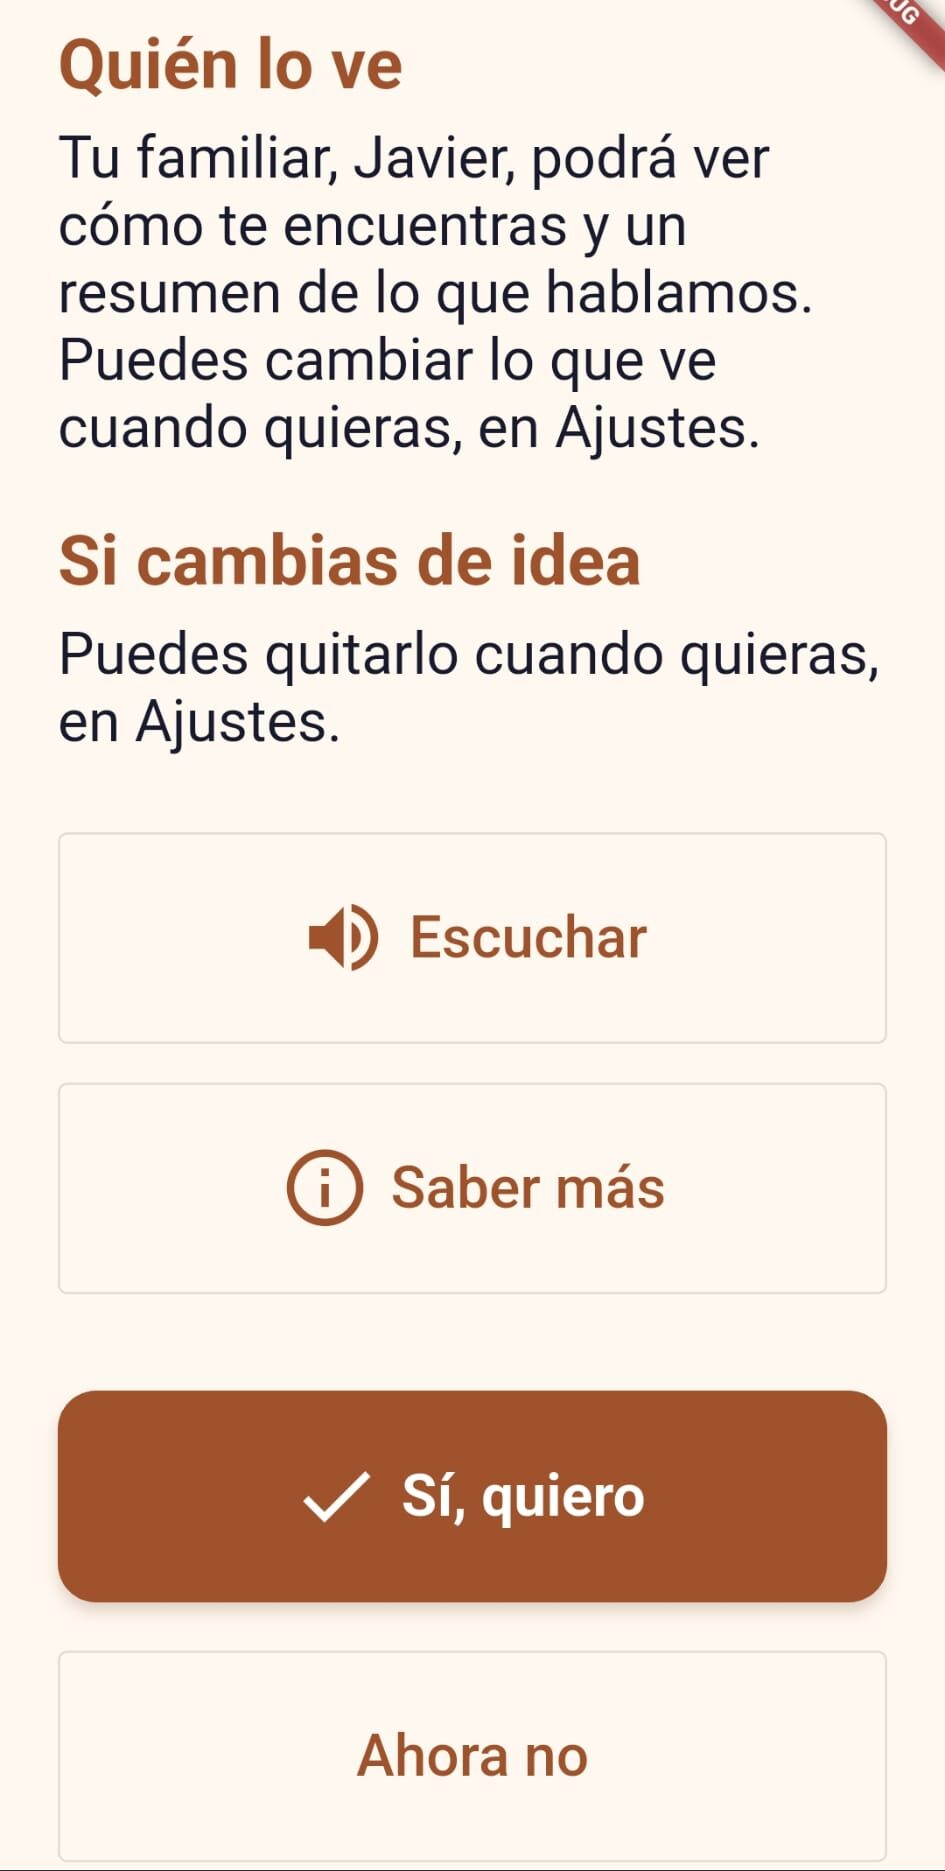
\includegraphics[width=\linewidth]{imagenes/manual/mayor-consentimiento-botones}
    \caption{Respuesta}
  \end{subfigure}
  \caption{Primeros pasos de la persona mayor.}
  \label{fig:manual-inicio}
\end{figure}

La primera vez que abra la aplicación, esta le preguntará cómo quiere entrar (\autoref{fig:manual-inicio}). Con <<Entrar con Google>> conserva todo aunque cambie de móvil; con <<Entrar sin registrarme>> no necesita ninguna cuenta, pero si borra la aplicación empezará de cero. Más adelante puede pasar a su cuenta de Google desde Ajustes. El enlace <<Soy el acompañante>> es para su familiar.

Después elija cómo quiere usarla. Con <<Usar por mi cuenta>> conversa con el asistente sin que nadie más vea nada. Con <<Vincular con mi familiar>> aparece un código de cuatro caracteres: dígaselo a su familiar para que lo escriba en su aplicación. Cuando lo haga, la pantalla cambiará sola.

Por último, el asistente le pregunta si quiere que guarde un resumen de sus conversaciones. La pantalla explica qué se guarda, qué recuerda el asistente y quién puede verlo; <<Escuchar>> se lo lee en voz alta y <<Saber más>> da todos los detalles. Puede contestar <<Sí, quiero>> o <<Ahora no>>. Si no acepta, puede conversar igualmente, pero no se guarda ningún resumen. Lo que conteste puede cambiarlo cuando quiera desde Ajustes.

\subsection{Conversar con el asistente}

\begin{figure}[!htb]\centering
  \begin{subfigure}[t]{0.27\textwidth}\centering
    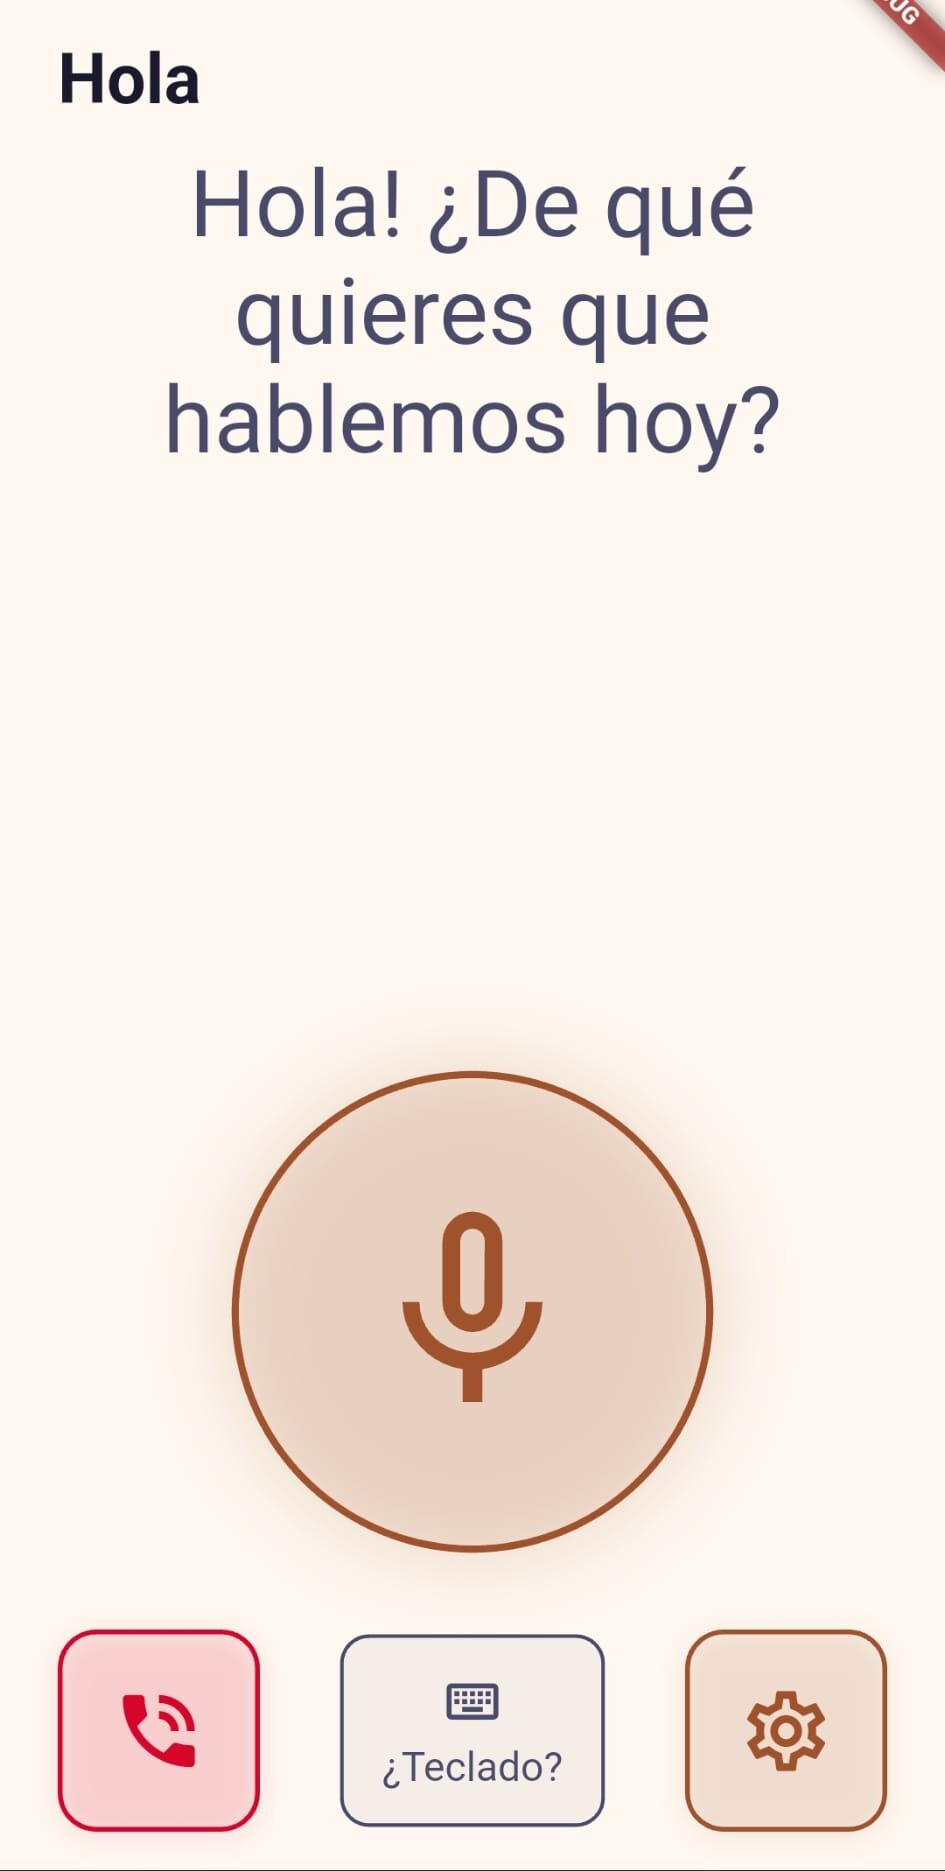
\includegraphics[width=\linewidth]{imagenes/manual/mayor-principal-voz}
    \caption{Pantalla principal}
  \end{subfigure}\hfill
  \begin{subfigure}[t]{0.27\textwidth}\centering
    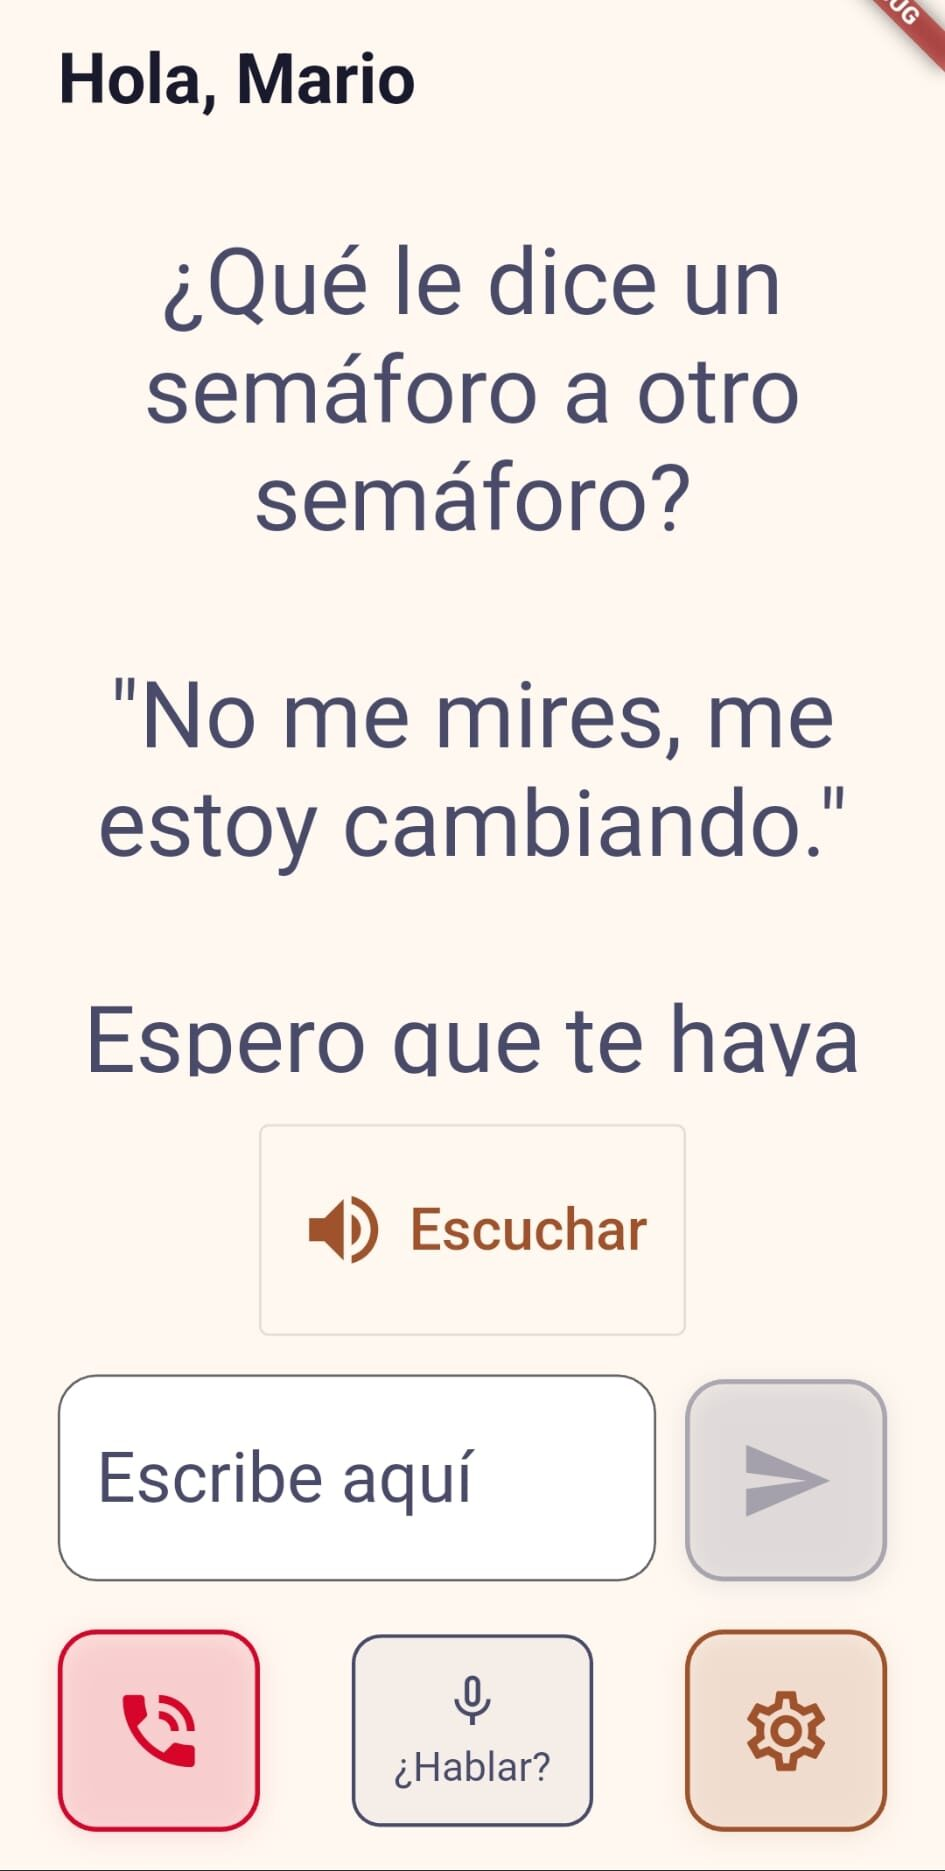
\includegraphics[width=\linewidth]{imagenes/manual/mayor-principal-teclado}
    \caption{Modo teclado}
  \end{subfigure}\hfill
  \begin{subfigure}[t]{0.27\textwidth}\centering
    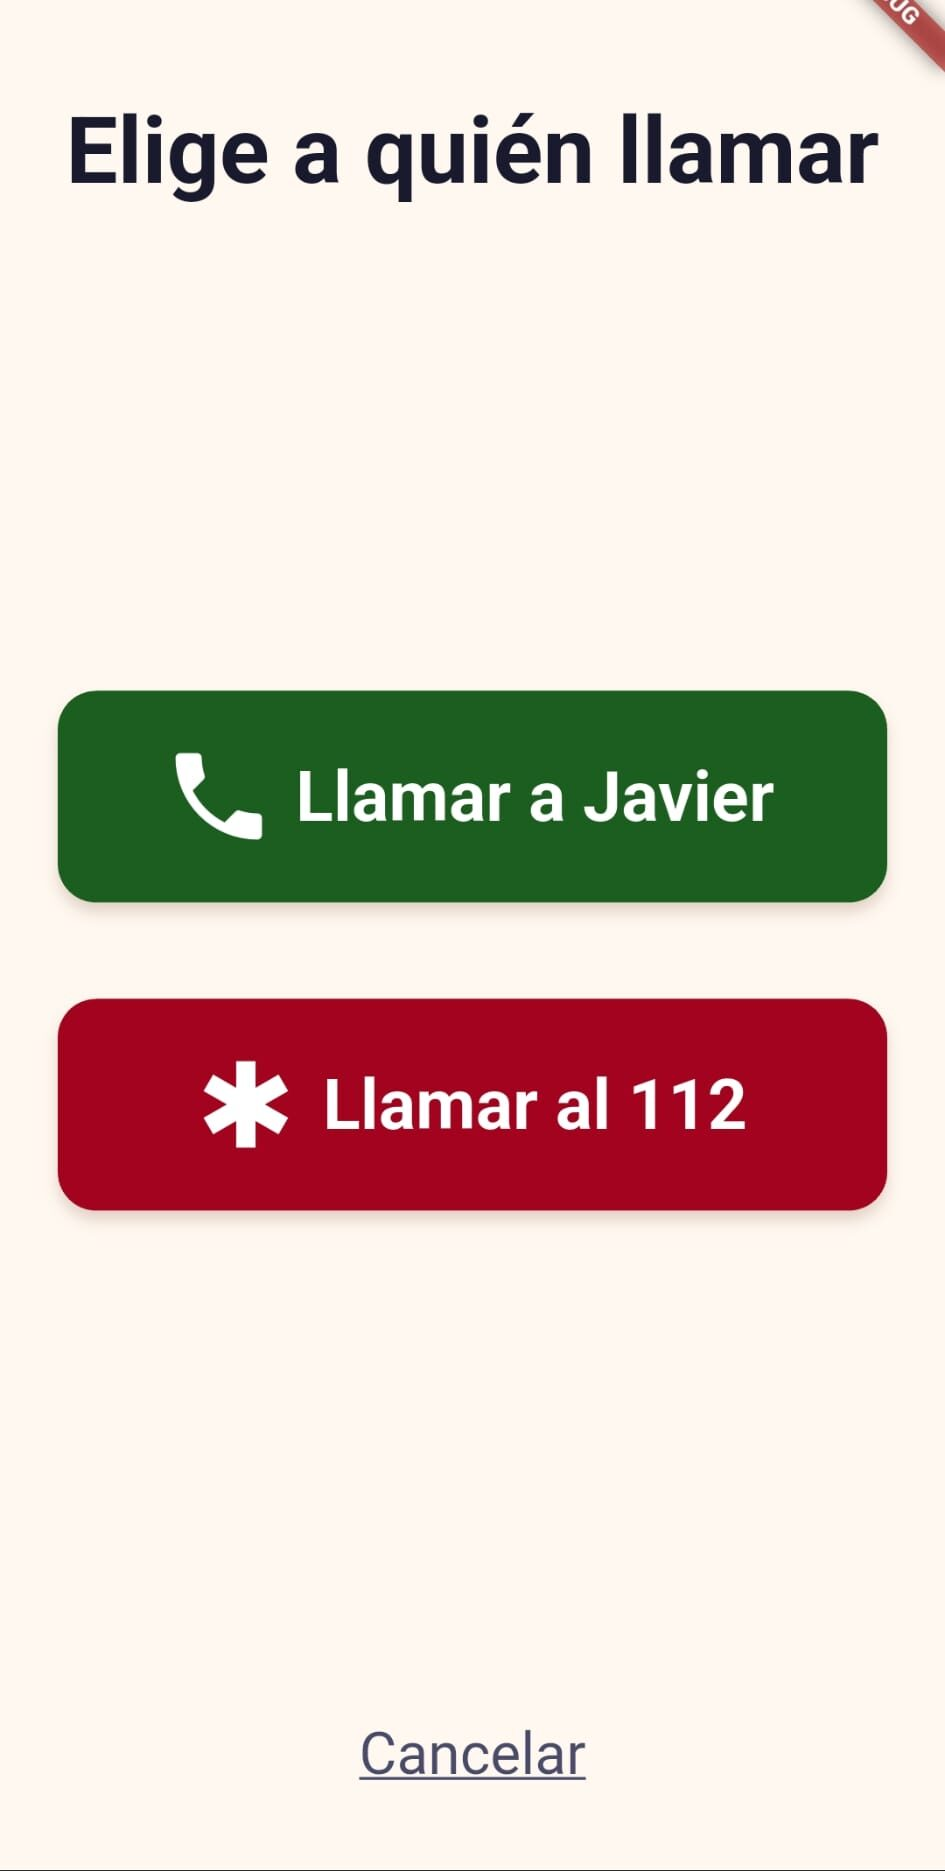
\includegraphics[width=\linewidth]{imagenes/manual/mayor-emergencia}
    \caption{Emergencia}
  \end{subfigure}
  \caption{Conversación y llamada de emergencia.}
  \label{fig:manual-principal}
\end{figure}

La pantalla principal tiene un solo botón grande, el del micrófono (\autoref{fig:manual-principal}). Tóquelo y hable con normalidad. Cuando se quede en silencio unos segundos, el asistente entiende que ha terminado y le contesta en voz alta; si no quiere esperar, toque otra vez el micrófono al acabar de hablar. Para seguir la conversación, vuelva a tocarlo. Si el asistente le corta antes de que termine, alargue el <<Tiempo que te espero>> en Ajustes.

También puede escribir. Toque <<¿Teclado?>>, escriba en el recuadro <<Escribe aquí>> y pulse la flecha de enviar. En este modo la respuesta no se lee sola: toque <<Escuchar>> para oírla. <<¿Hablar?>> vuelve al micrófono.

Abajo hay siempre tres botones: el teléfono rojo, para pedir ayuda; el del centro, para cambiar entre voz y teclado; y la rueda, para los ajustes. Cuando ya hay alguna conversación resumida, aparece además el botón <<Mi semana>> (apartado~\ref{sec:manual-mi-semana}).

\subsection{Pedir ayuda}

El botón rojo del teléfono abre la pantalla de emergencia. <<Llamar a>>, seguido de un nombre, llama a su familiar o a su contacto de emergencia, y <<Llamar al 112>> llama a emergencias. El móvil abre el marcador con el número ya escrito y solo queda pulsar el botón de llamar. <<Cancelar>> vuelve a la conversación.

Si está vinculado, su contacto de emergencia es su familiar; si usa la aplicación por su cuenta, elíjalo en Ajustes, dentro de <<Mis datos>>. El asistente no avisa a nadie por sí solo: si necesita ayuda, use siempre este botón.

\subsection{Ajustes}

\begin{figure}[!htb]\centering
  \begin{subfigure}[t]{0.165\textwidth}\centering
    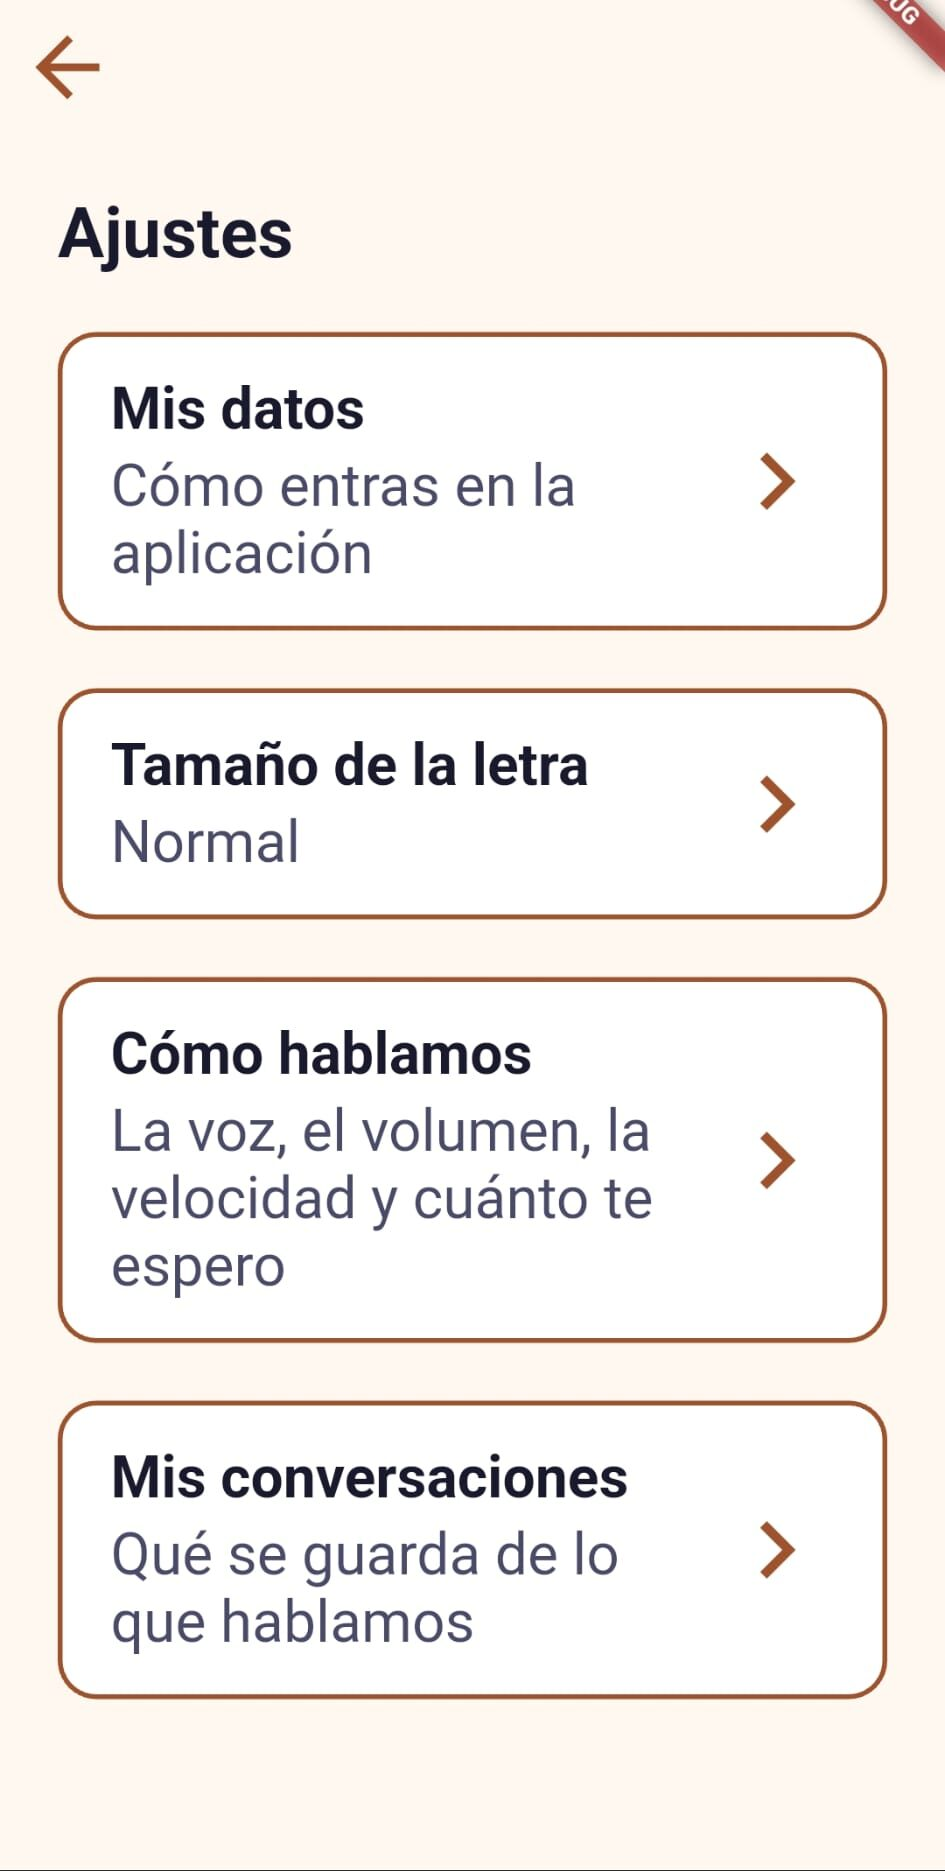
\includegraphics[width=\linewidth]{imagenes/manual/mayor-ajustes}
    \caption{Ajustes}
  \end{subfigure}\manualhueco
  \begin{subfigure}[t]{0.165\textwidth}\centering
    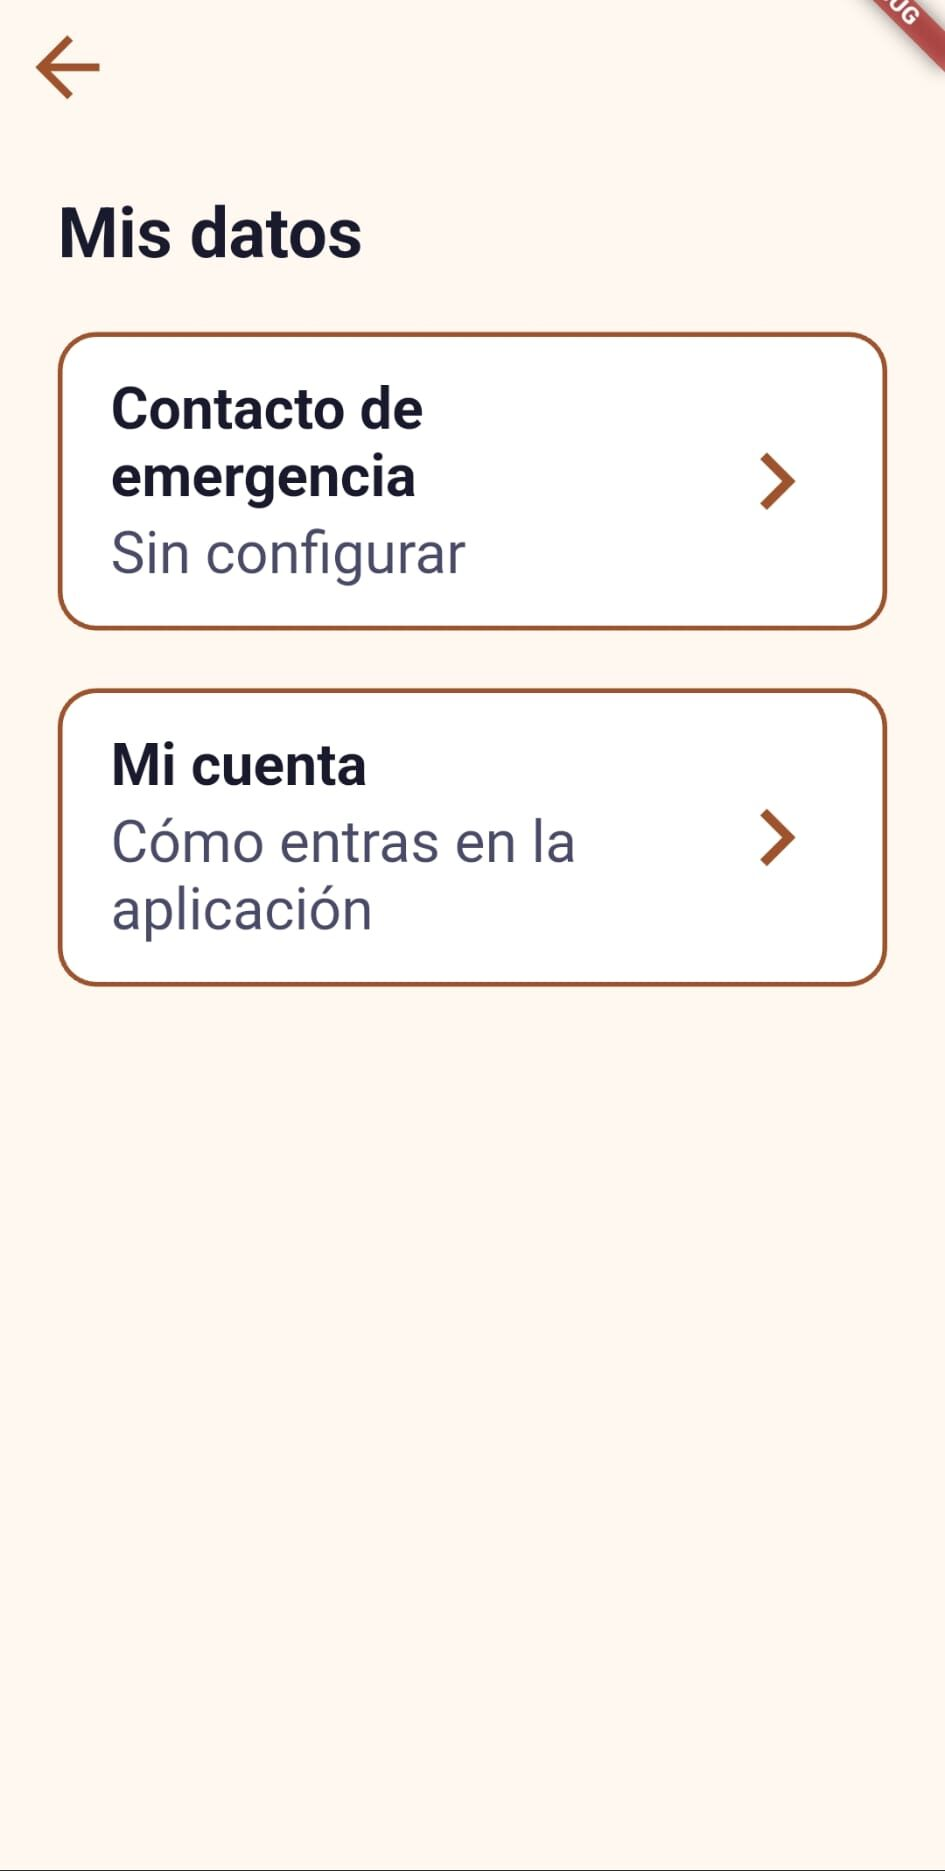
\includegraphics[width=\linewidth]{imagenes/manual/mayor-mis-datos}
    \caption{Mis datos}
  \end{subfigure}\manualhueco
  \begin{subfigure}[t]{0.165\textwidth}\centering
    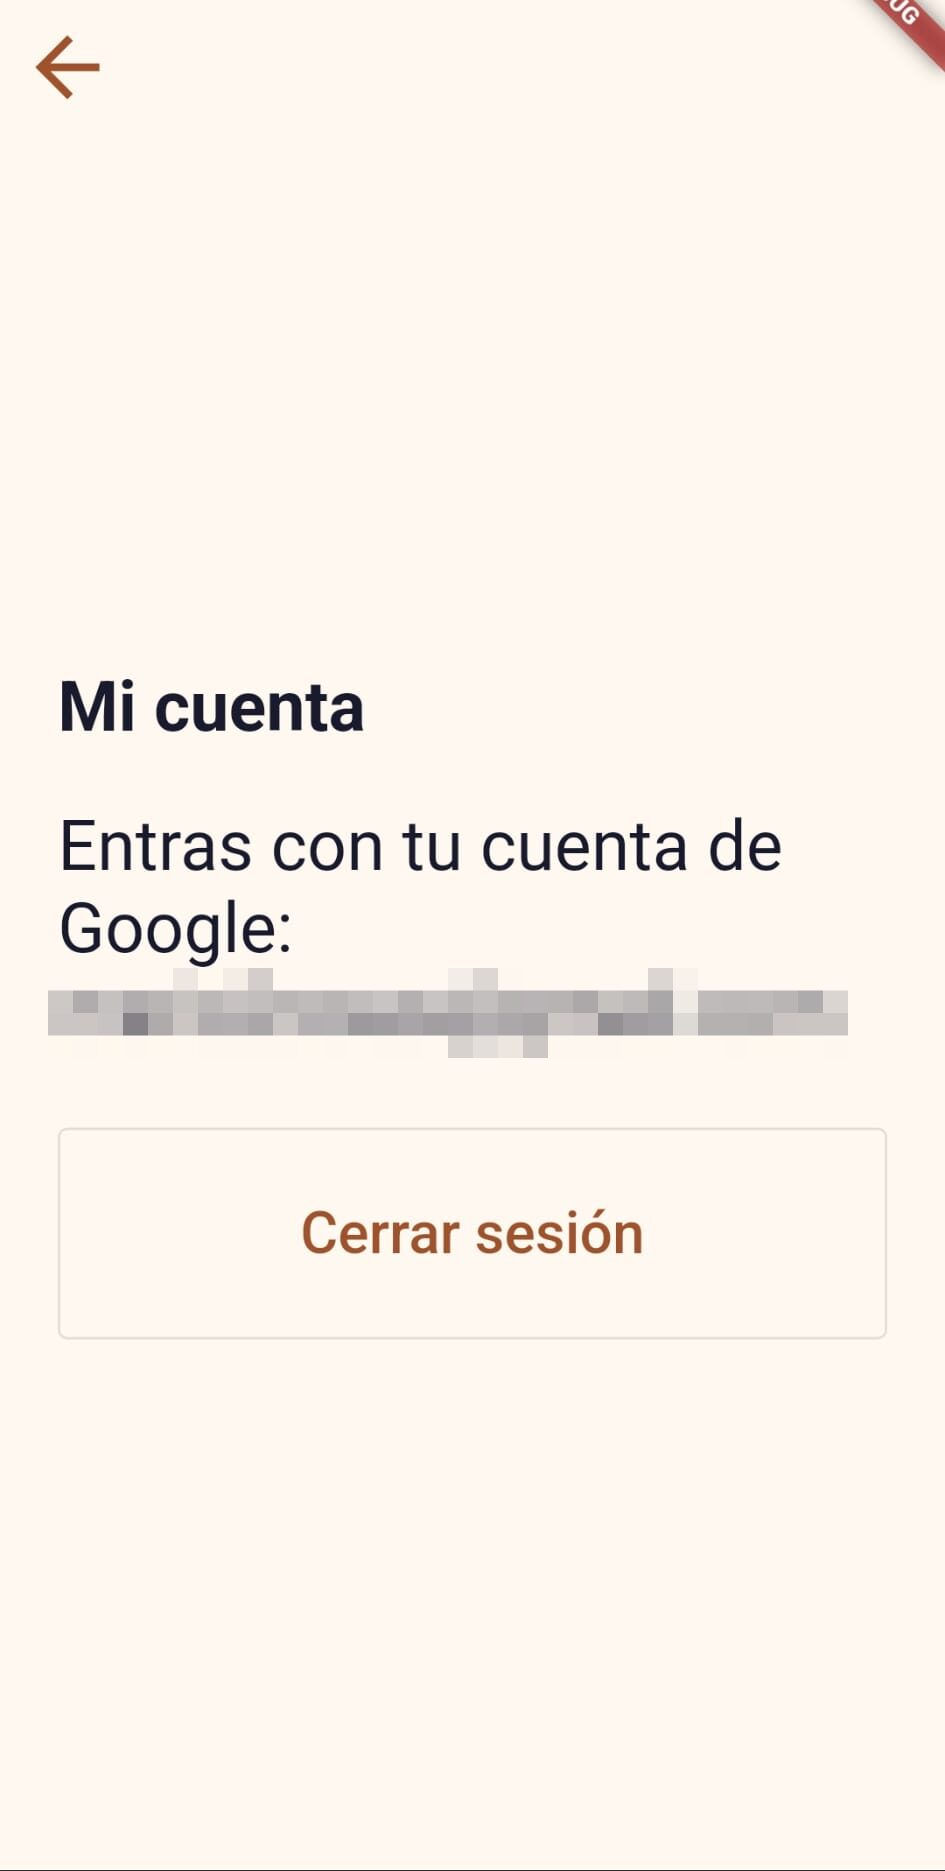
\includegraphics[width=\linewidth]{imagenes/manual/mayor-mi-cuenta}
    \caption{Mi cuenta}
  \end{subfigure}\manualhueco
  \begin{subfigure}[t]{0.165\textwidth}\centering
    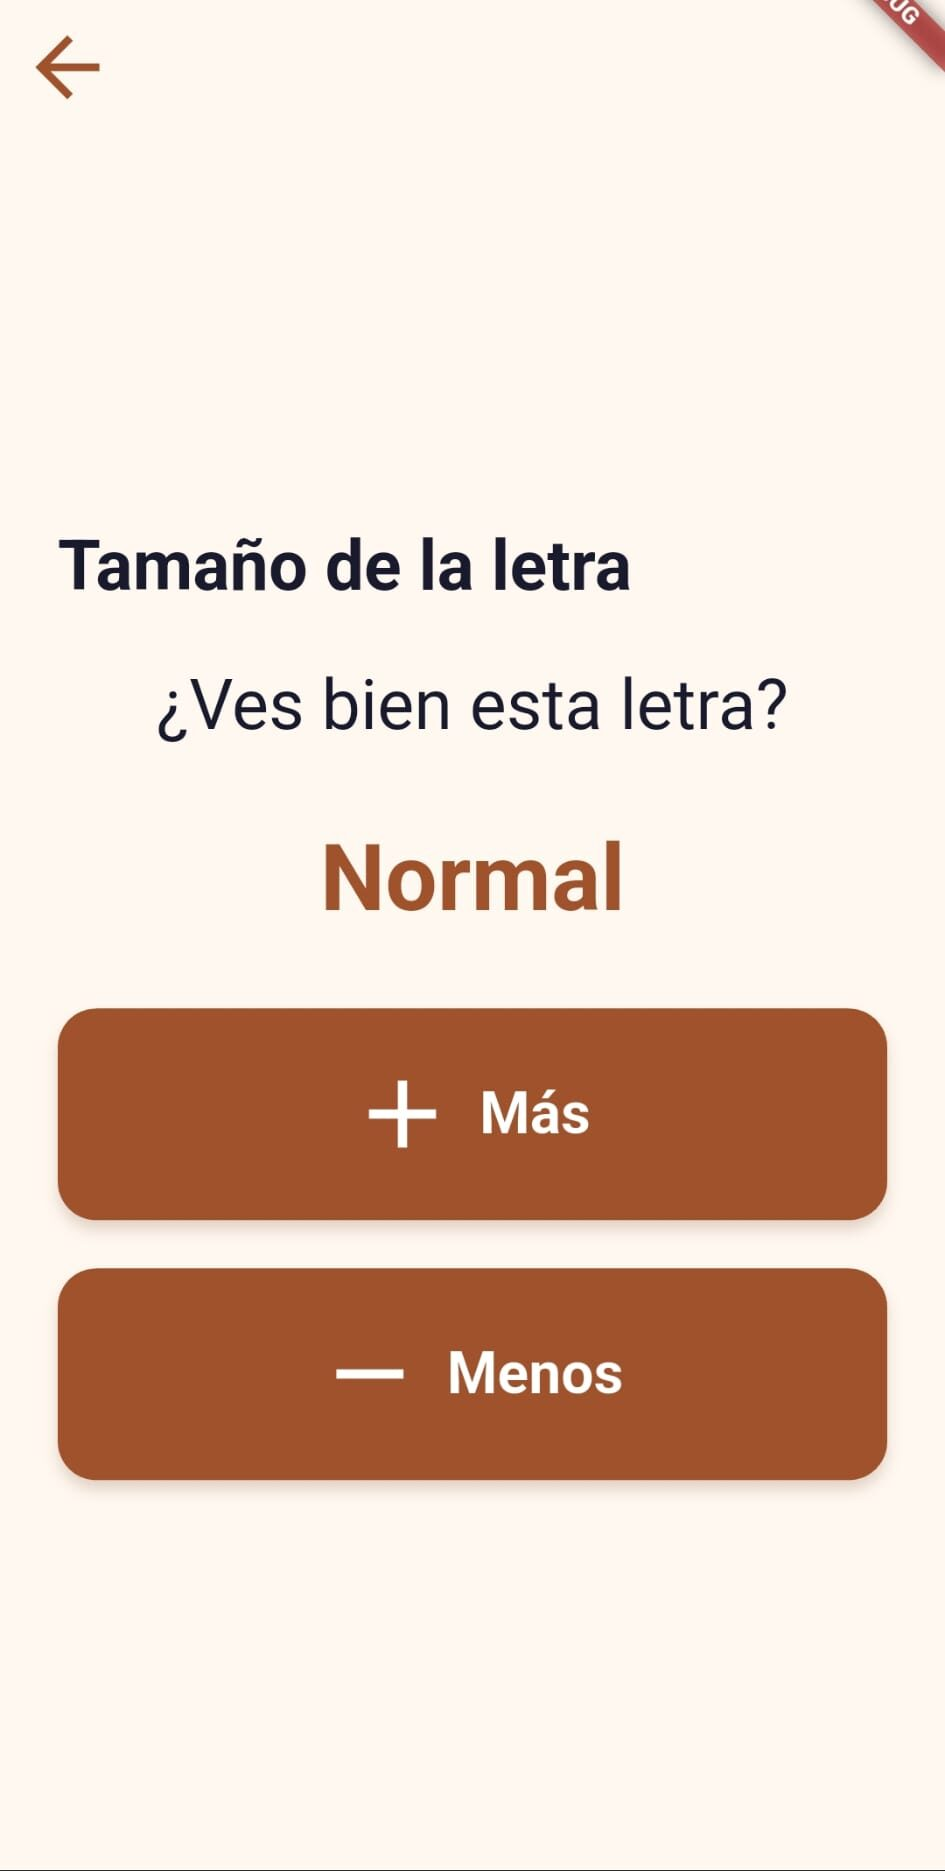
\includegraphics[width=\linewidth]{imagenes/manual/mayor-letra-normal}
    \caption{Letra normal}
  \end{subfigure}\manualhueco
  \begin{subfigure}[t]{0.165\textwidth}\centering
    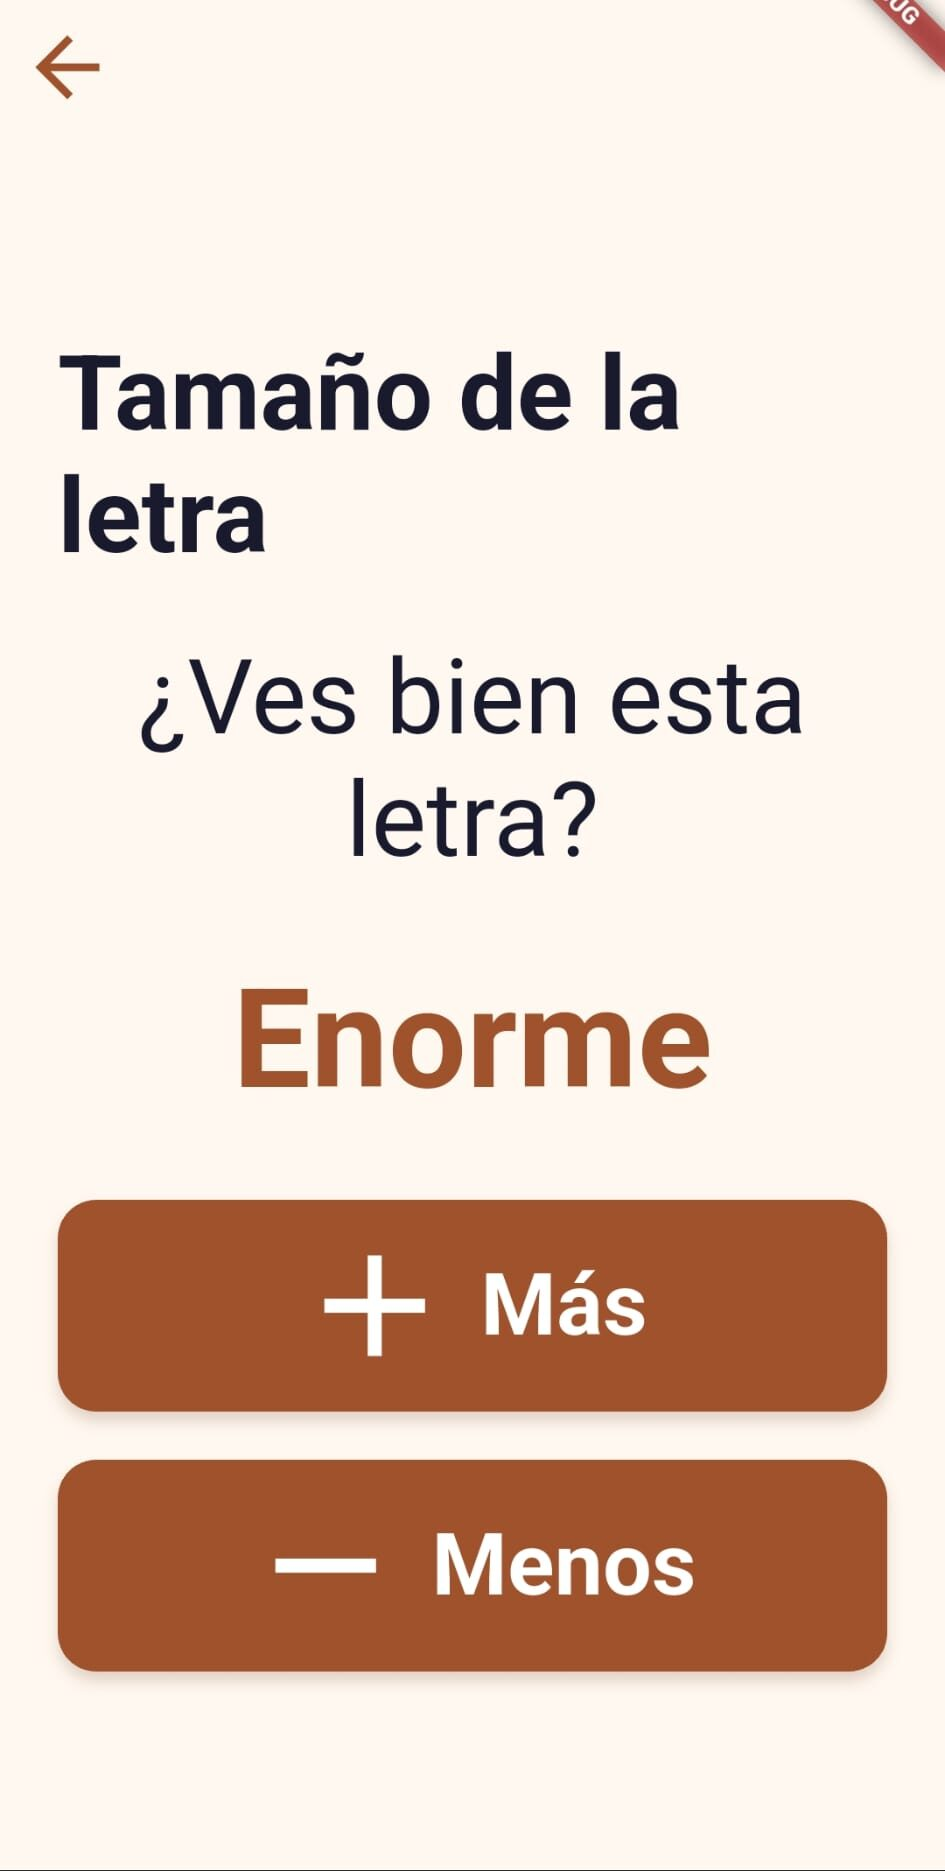
\includegraphics[width=\linewidth]{imagenes/manual/mayor-letra-enorme}
    \caption{Letra enorme}
  \end{subfigure}

  \medskip
  \begin{subfigure}[t]{0.165\textwidth}\centering
    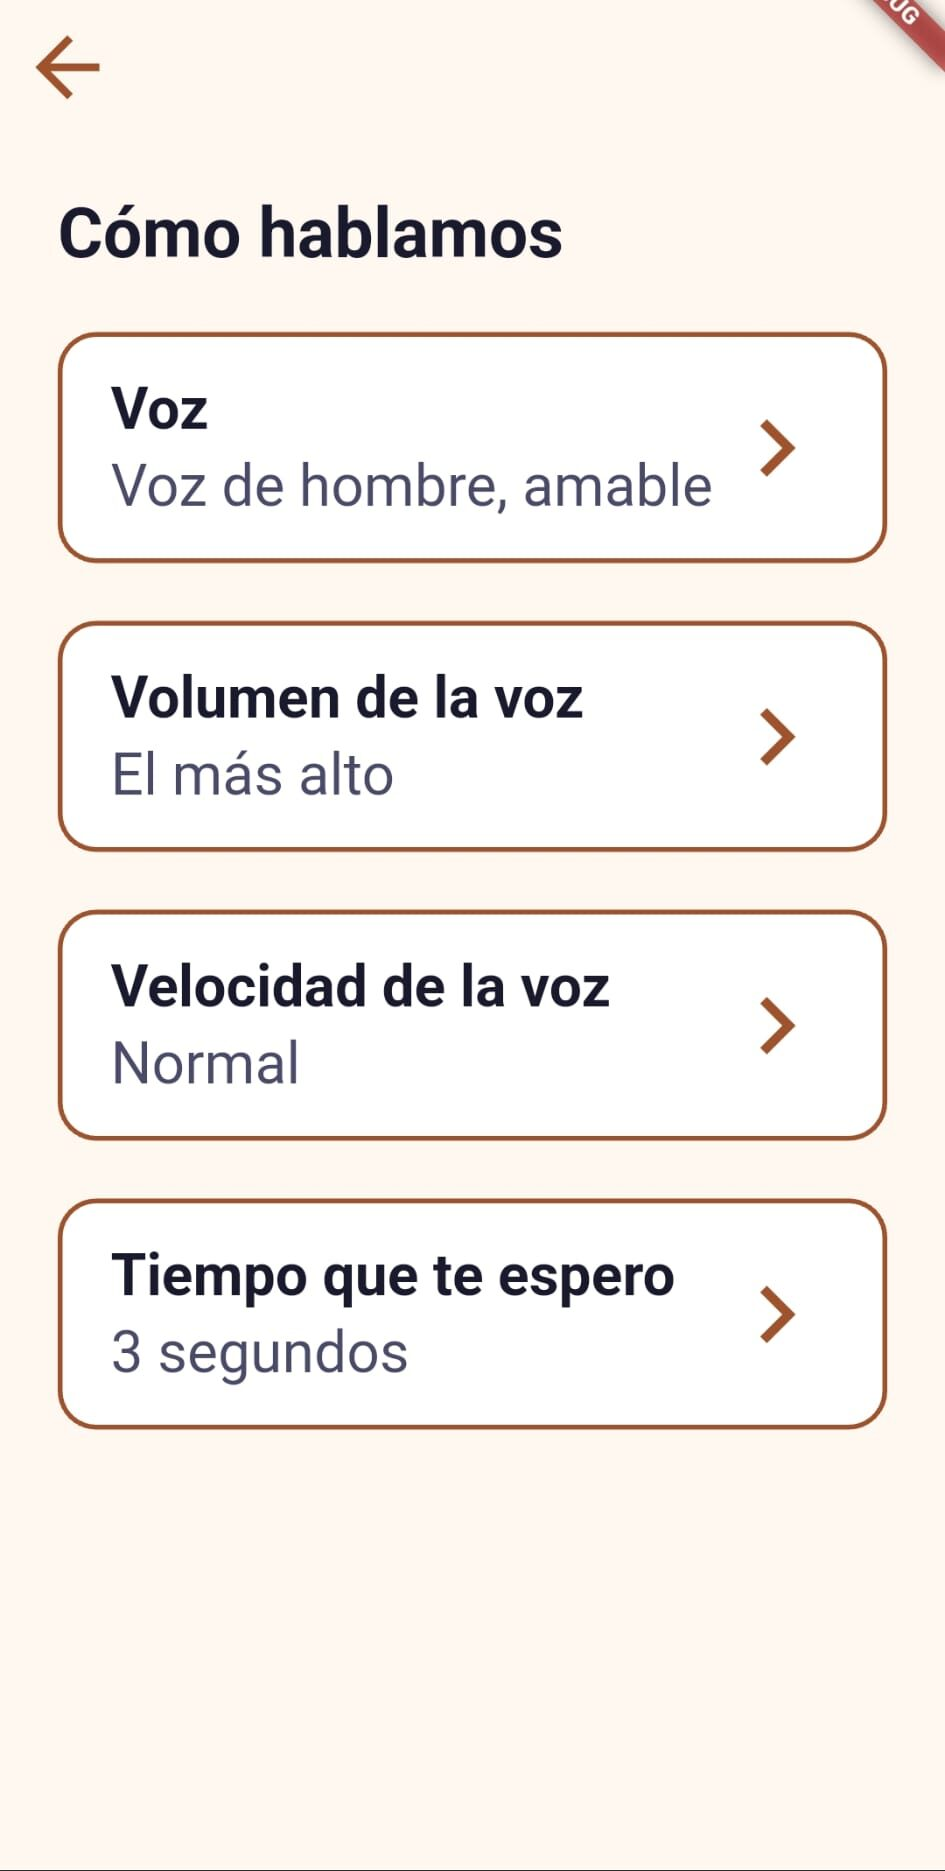
\includegraphics[width=\linewidth]{imagenes/manual/mayor-como-hablamos}
    \captionsetup{justification=centering}\caption{Cómo hablamos}
  \end{subfigure}\manualhueco
  \begin{subfigure}[t]{0.165\textwidth}\centering
    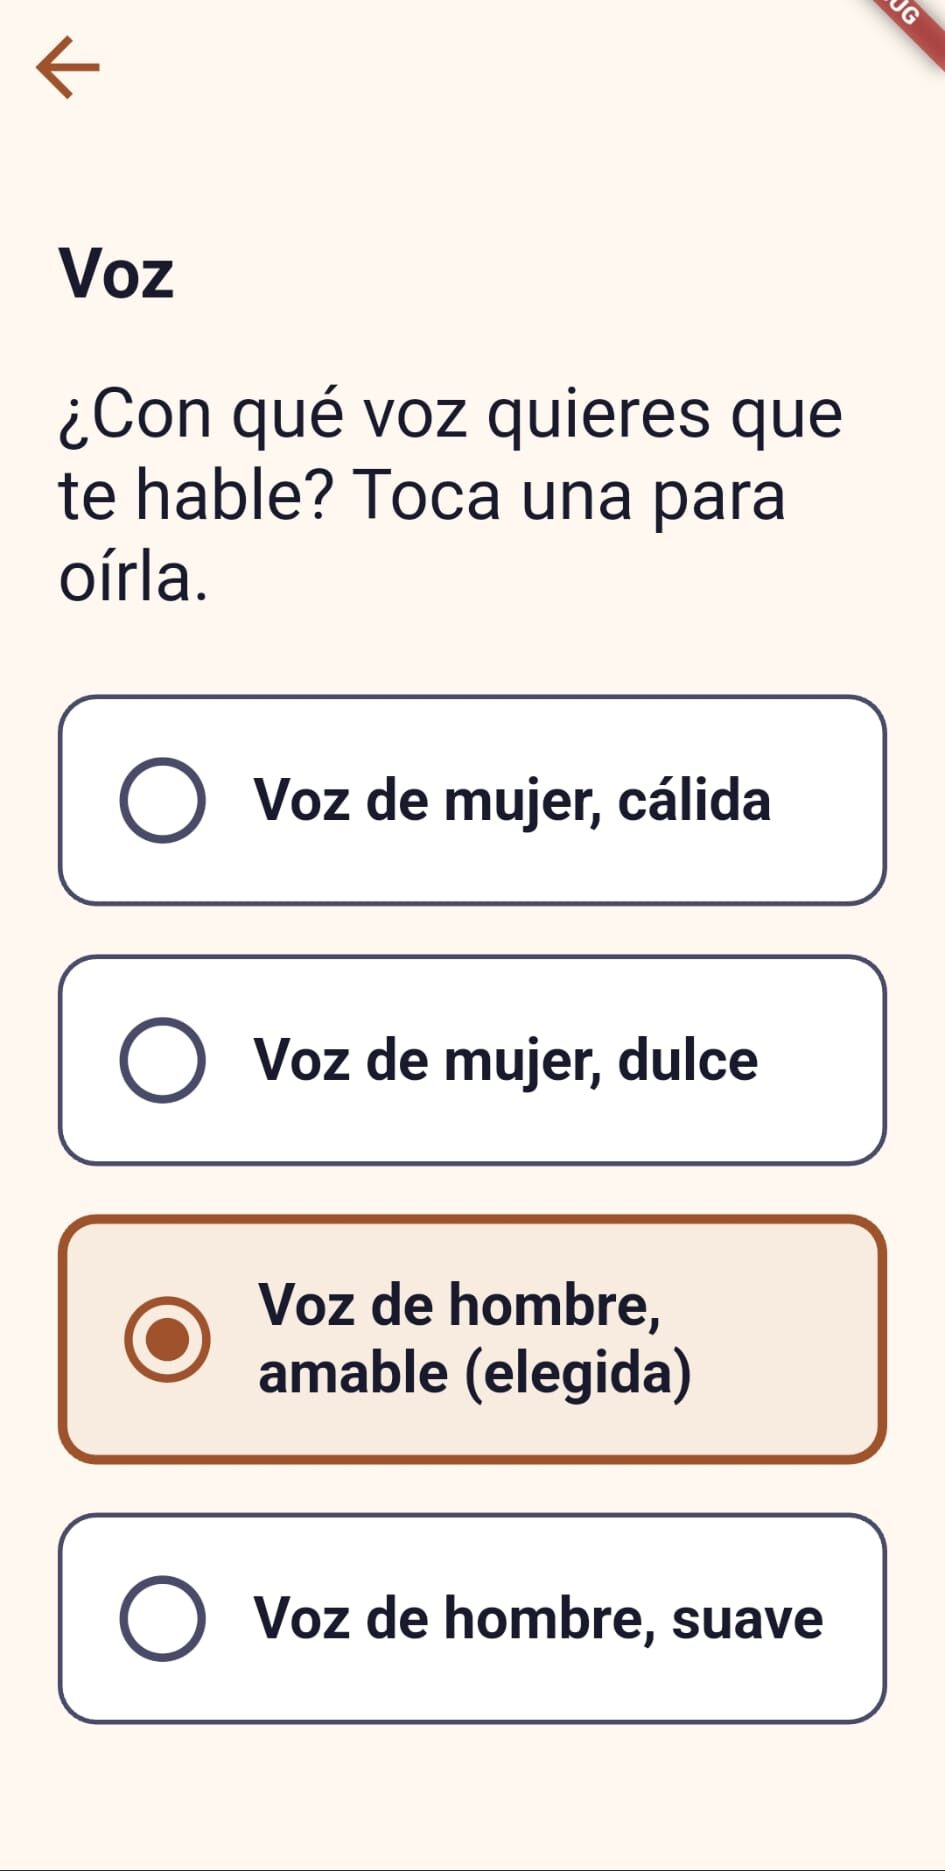
\includegraphics[width=\linewidth]{imagenes/manual/mayor-voz}
    \caption{Voz}
  \end{subfigure}\manualhueco
  \begin{subfigure}[t]{0.165\textwidth}\centering
    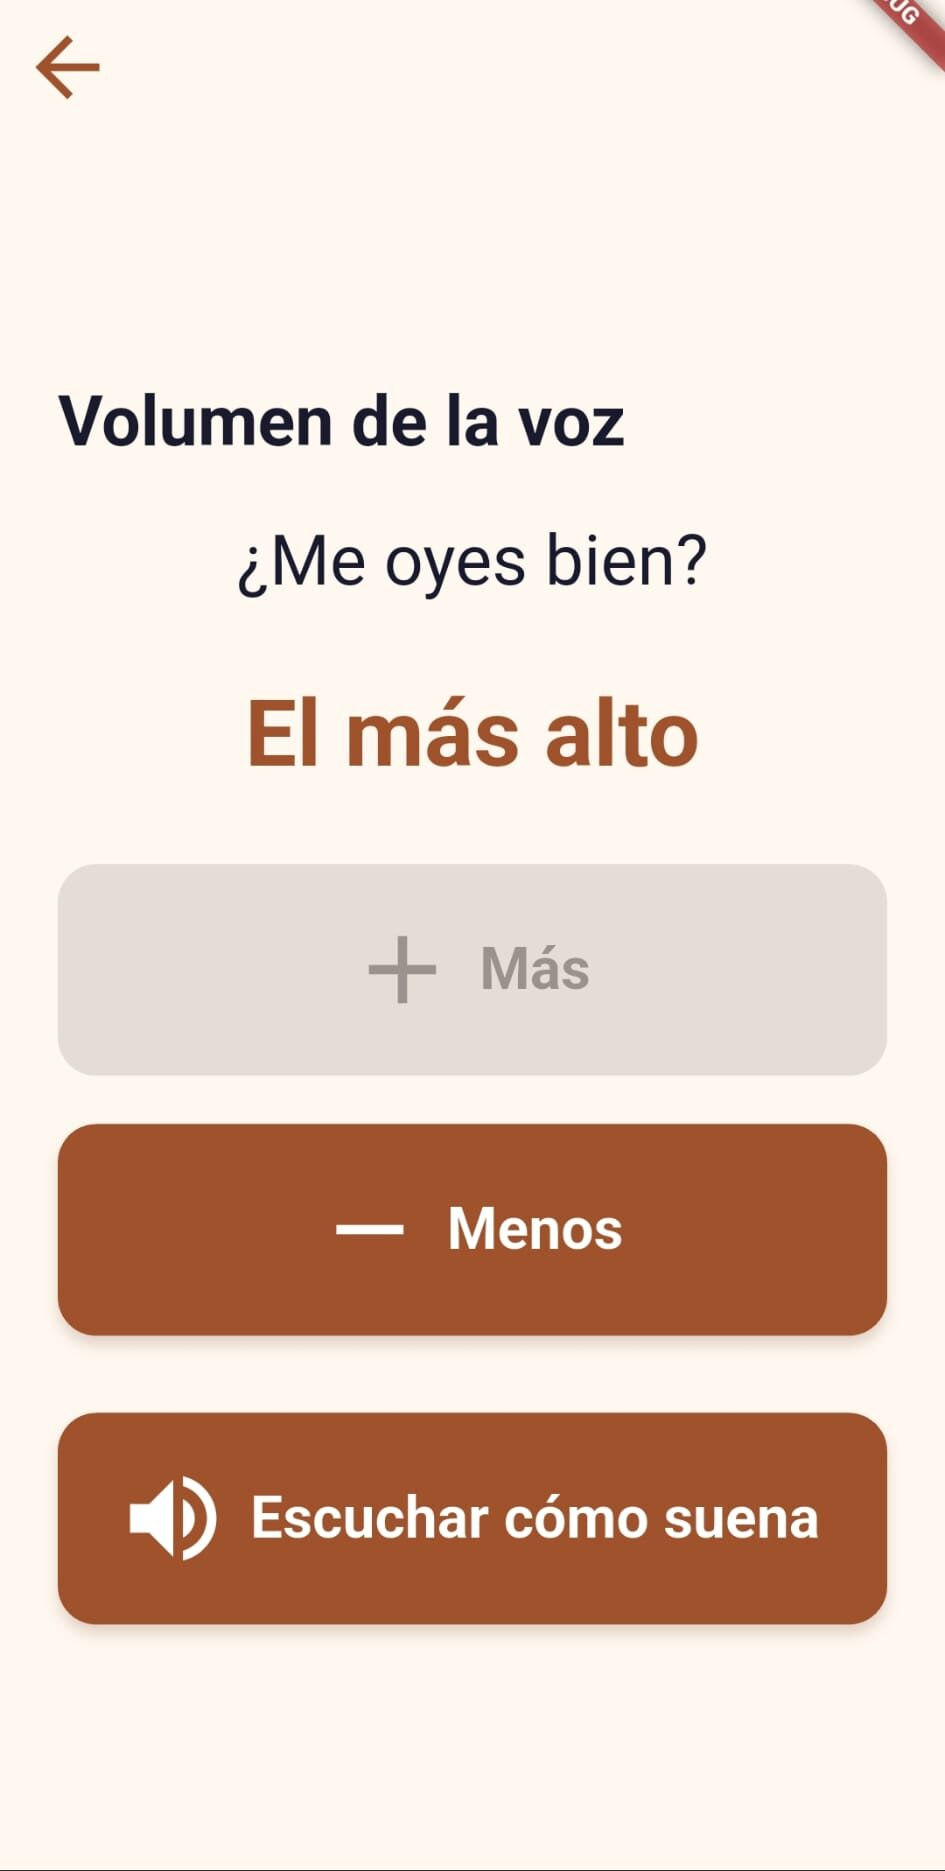
\includegraphics[width=\linewidth]{imagenes/manual/mayor-volumen}
    \caption{Volumen}
  \end{subfigure}\manualhueco
  \begin{subfigure}[t]{0.165\textwidth}\centering
    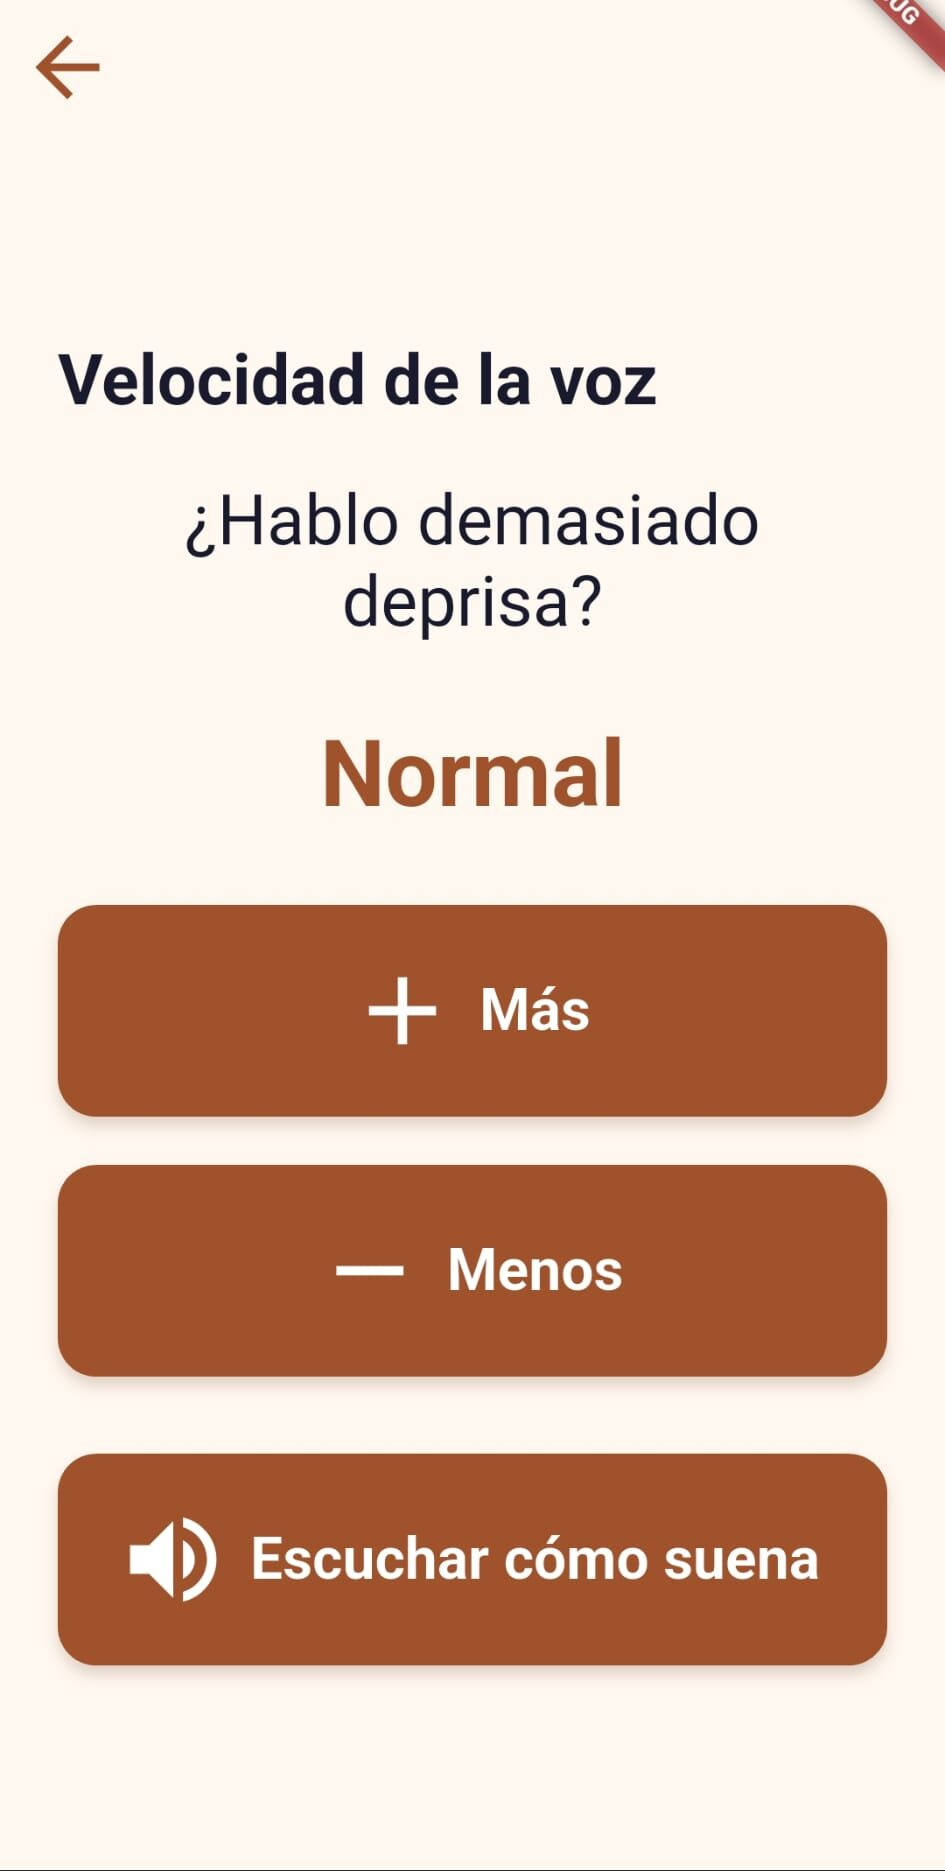
\includegraphics[width=\linewidth]{imagenes/manual/mayor-velocidad}
    \caption{Velocidad}
  \end{subfigure}\manualhueco
  \begin{subfigure}[t]{0.165\textwidth}\centering
    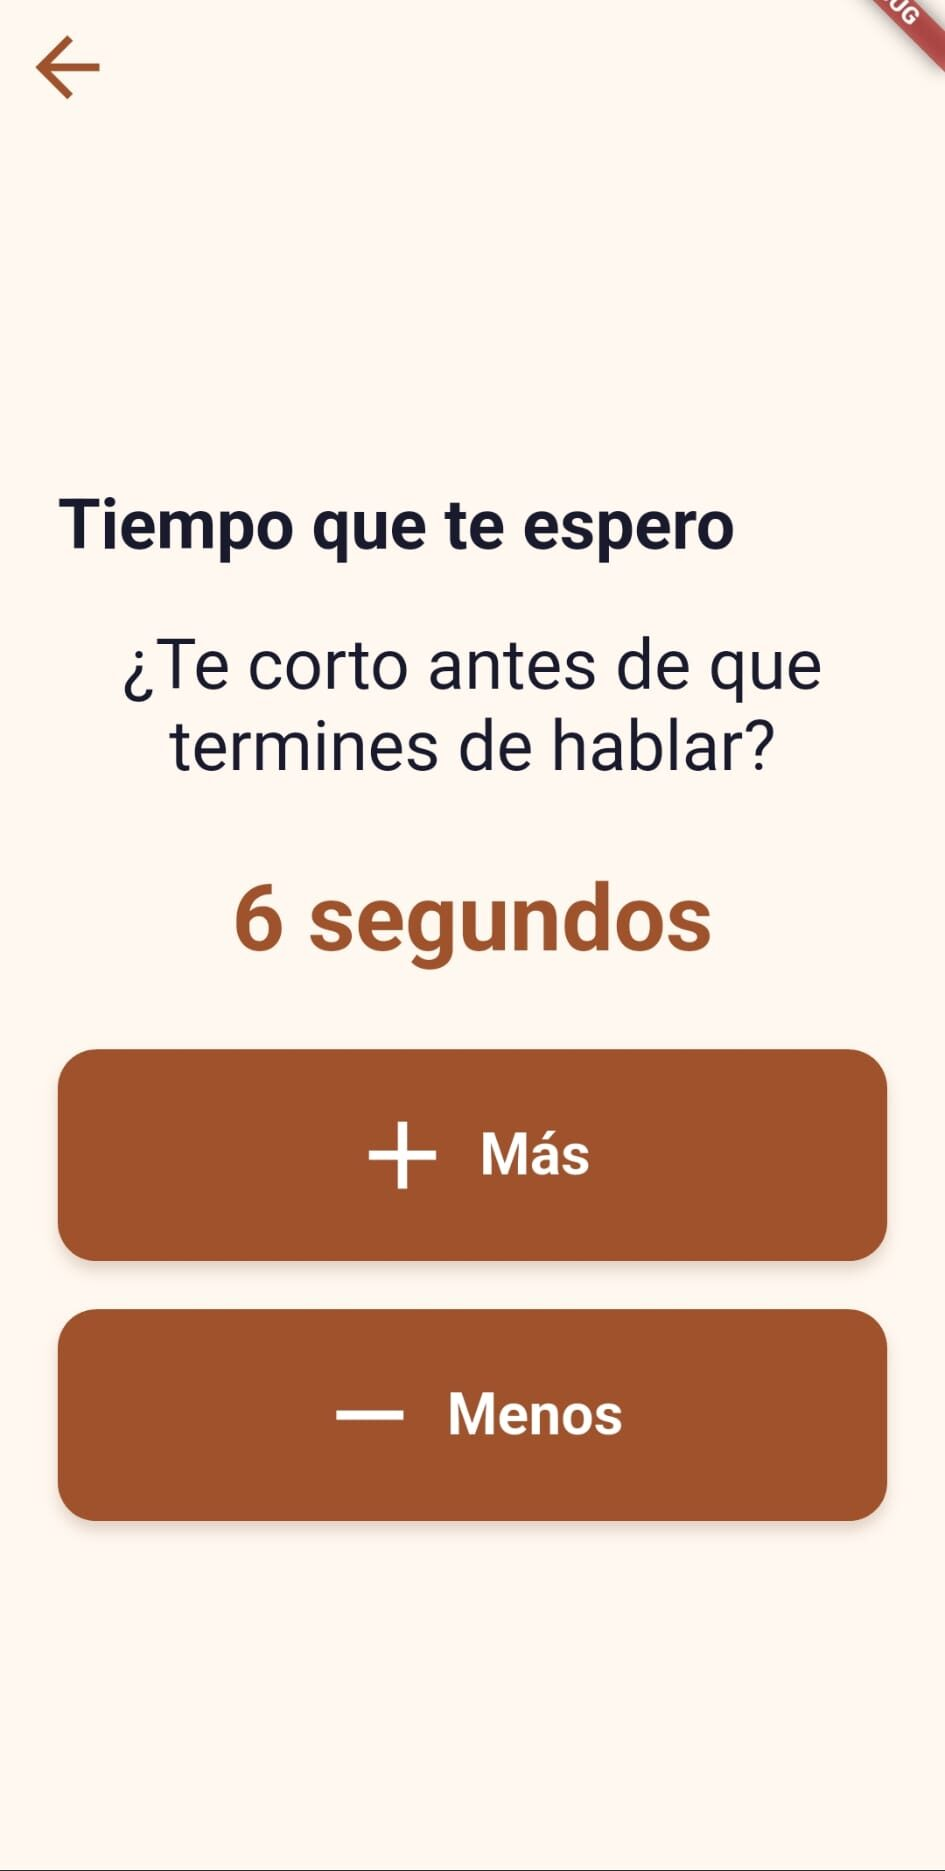
\includegraphics[width=\linewidth]{imagenes/manual/mayor-espera}
    \caption{Espera}
  \end{subfigure}
  \caption{Ajustes de la persona mayor.}
  \label{fig:manual-ajustes}
\end{figure}

La rueda de abajo a la derecha abre los ajustes, agrupados en cuatro apartados (\autoref{fig:manual-ajustes}). Todo se cambia con botones grandes, como <<Más>> y <<Menos>>, y los cambios se aplican al momento. La flecha de arriba a la izquierda vuelve a la pantalla anterior.

\begin{itemize}
  \item \textbf{Mis datos.} Su contacto de emergencia, si usa la aplicación por su cuenta, y <<Mi cuenta>>, que indica cómo entra en la aplicación. Si entró sin registrarse, desde ahí puede guardar su cuenta con Google para no perder nada al cambiar de móvil; si entra con Google, puede cerrar la sesión.
  \item \textbf{Tamaño de la letra.} La frase <<¿Ves bien esta letra?>> crece o encoge según pulse, para que compruebe con qué tamaño lee mejor.
  \item \textbf{Cómo hablamos.} La voz del asistente (al tocar una, la oye), el volumen, la velocidad y el tiempo que espera en silencio antes de contestar. El volumen y la velocidad se prueban con <<Escuchar cómo suena>>.
  \item \textbf{Mis conversaciones.} Qué se guarda de lo que hablan, como se explica a continuación.
\end{itemize}

\subsection{Mis conversaciones y <<Mi semana>>}
\label{sec:manual-mi-semana}

En <<Mis conversaciones>> decide qué se guarda de lo que habla con el asistente (\autoref{fig:manual-conversaciones}):

\begin{figure}[!htb]\centering
  \begin{subfigure}[t]{0.165\textwidth}\centering
    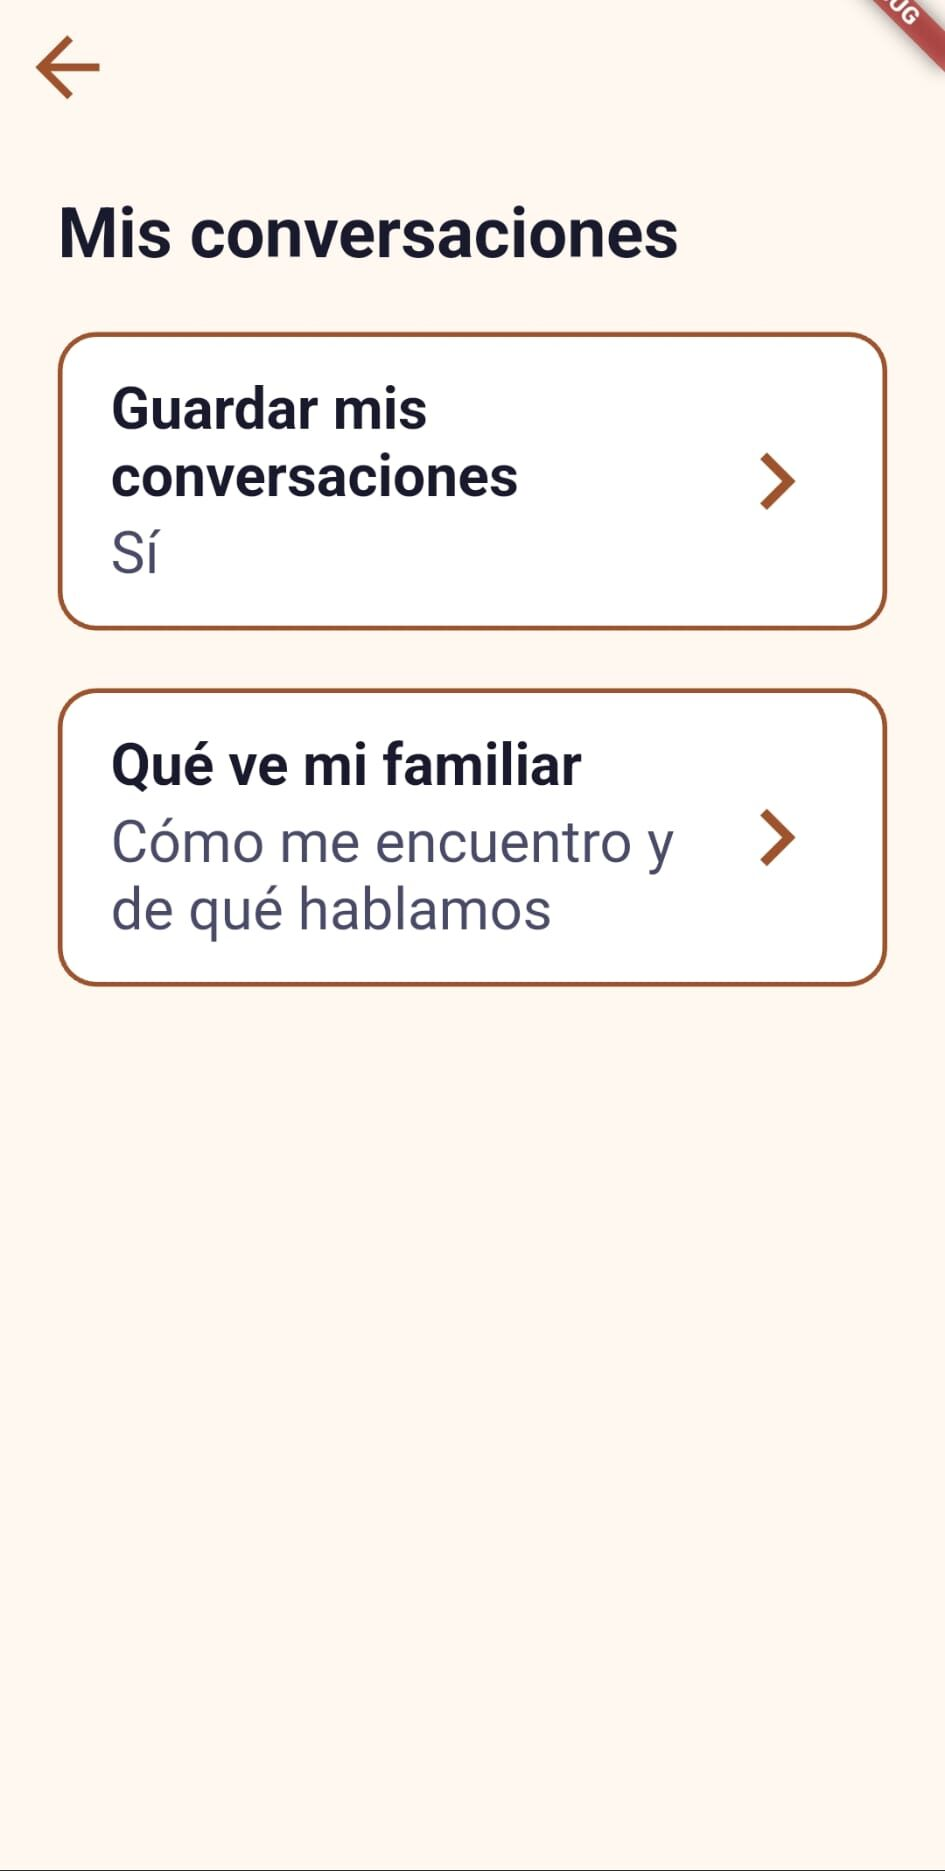
\includegraphics[width=\linewidth]{imagenes/manual/mayor-conversaciones}
    \caption{Opciones}
  \end{subfigure}\manualhueco
  \begin{subfigure}[t]{0.165\textwidth}\centering
    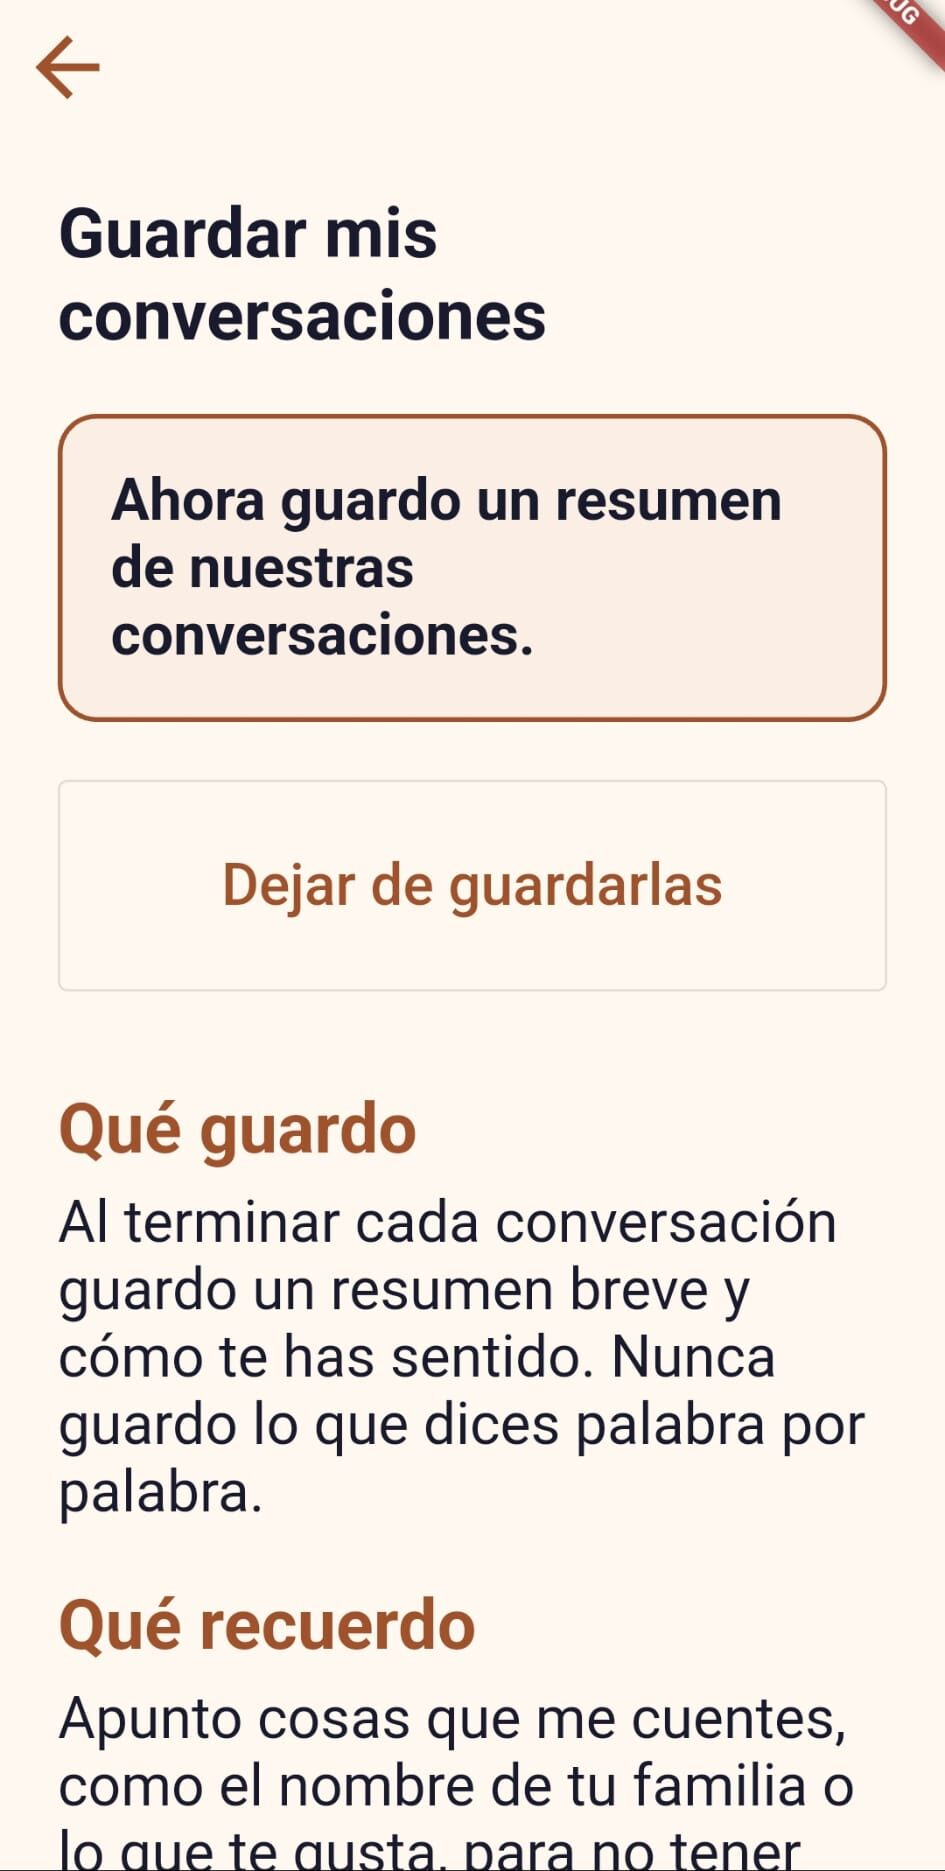
\includegraphics[width=\linewidth]{imagenes/manual/mayor-guardar}
    \caption{Guardar}
  \end{subfigure}\manualhueco
  \begin{subfigure}[t]{0.165\textwidth}\centering
    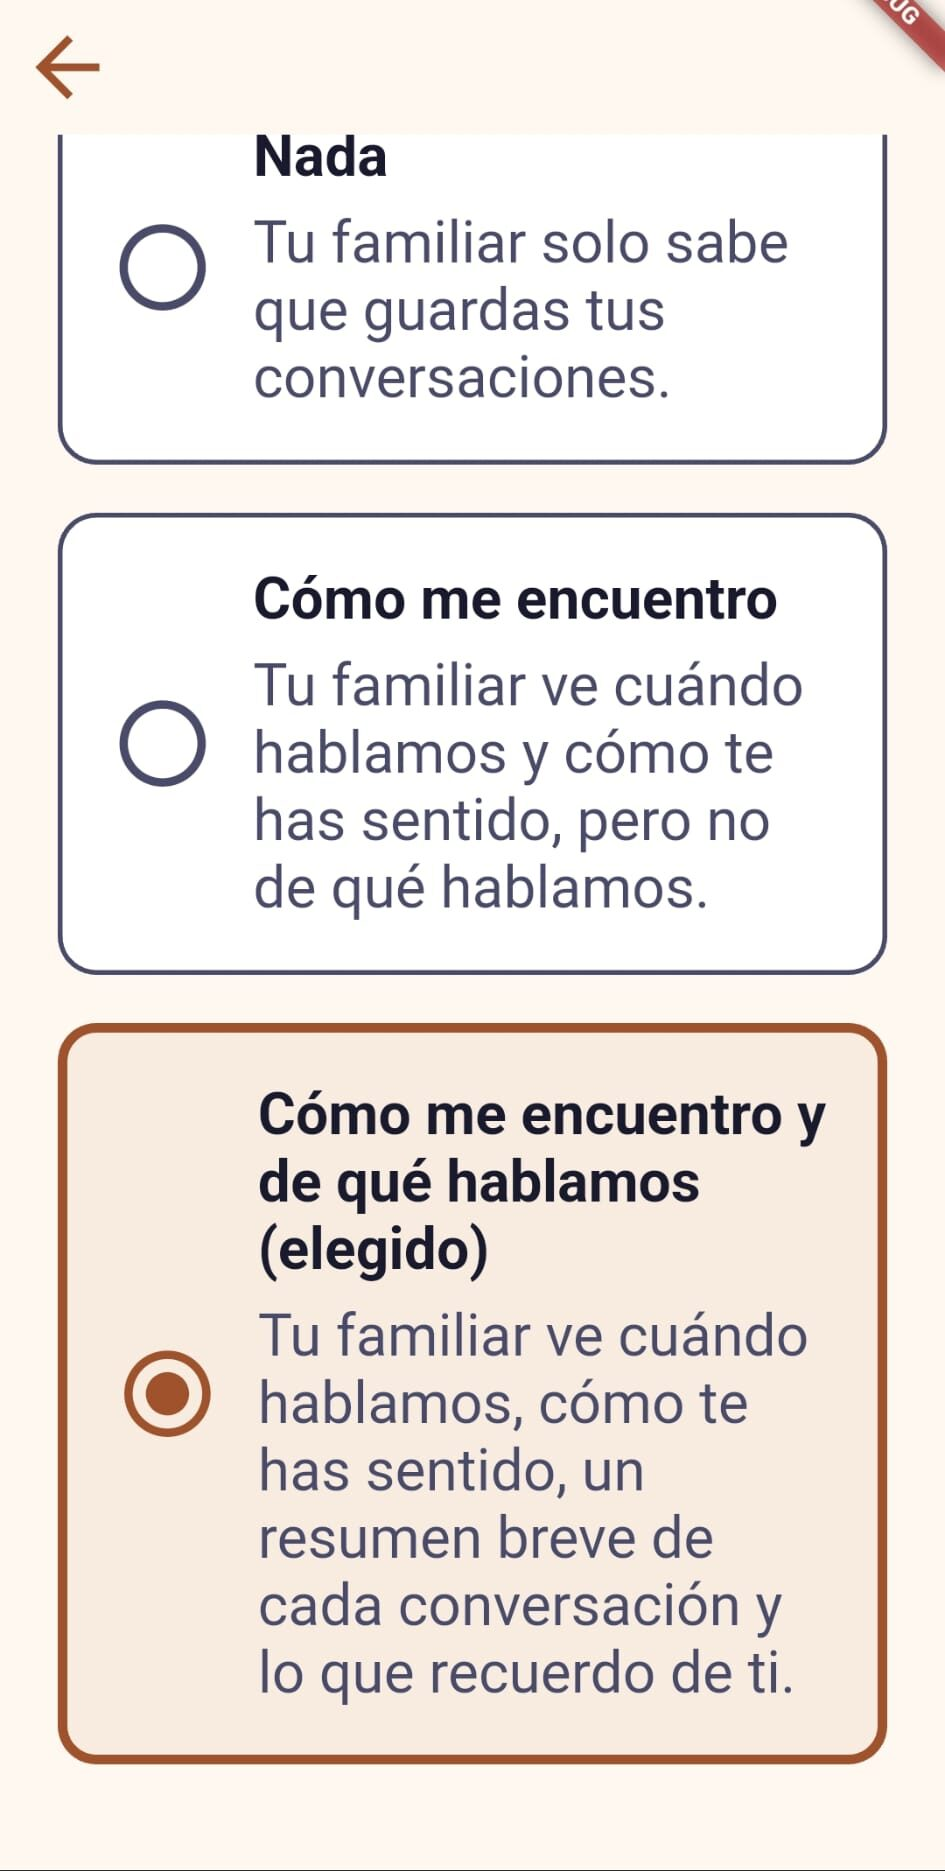
\includegraphics[width=\linewidth]{imagenes/manual/mayor-que-ve-familiar}
    \caption{Qué comparte}
  \end{subfigure}\manualhueco
  \begin{subfigure}[t]{0.165\textwidth}\centering
    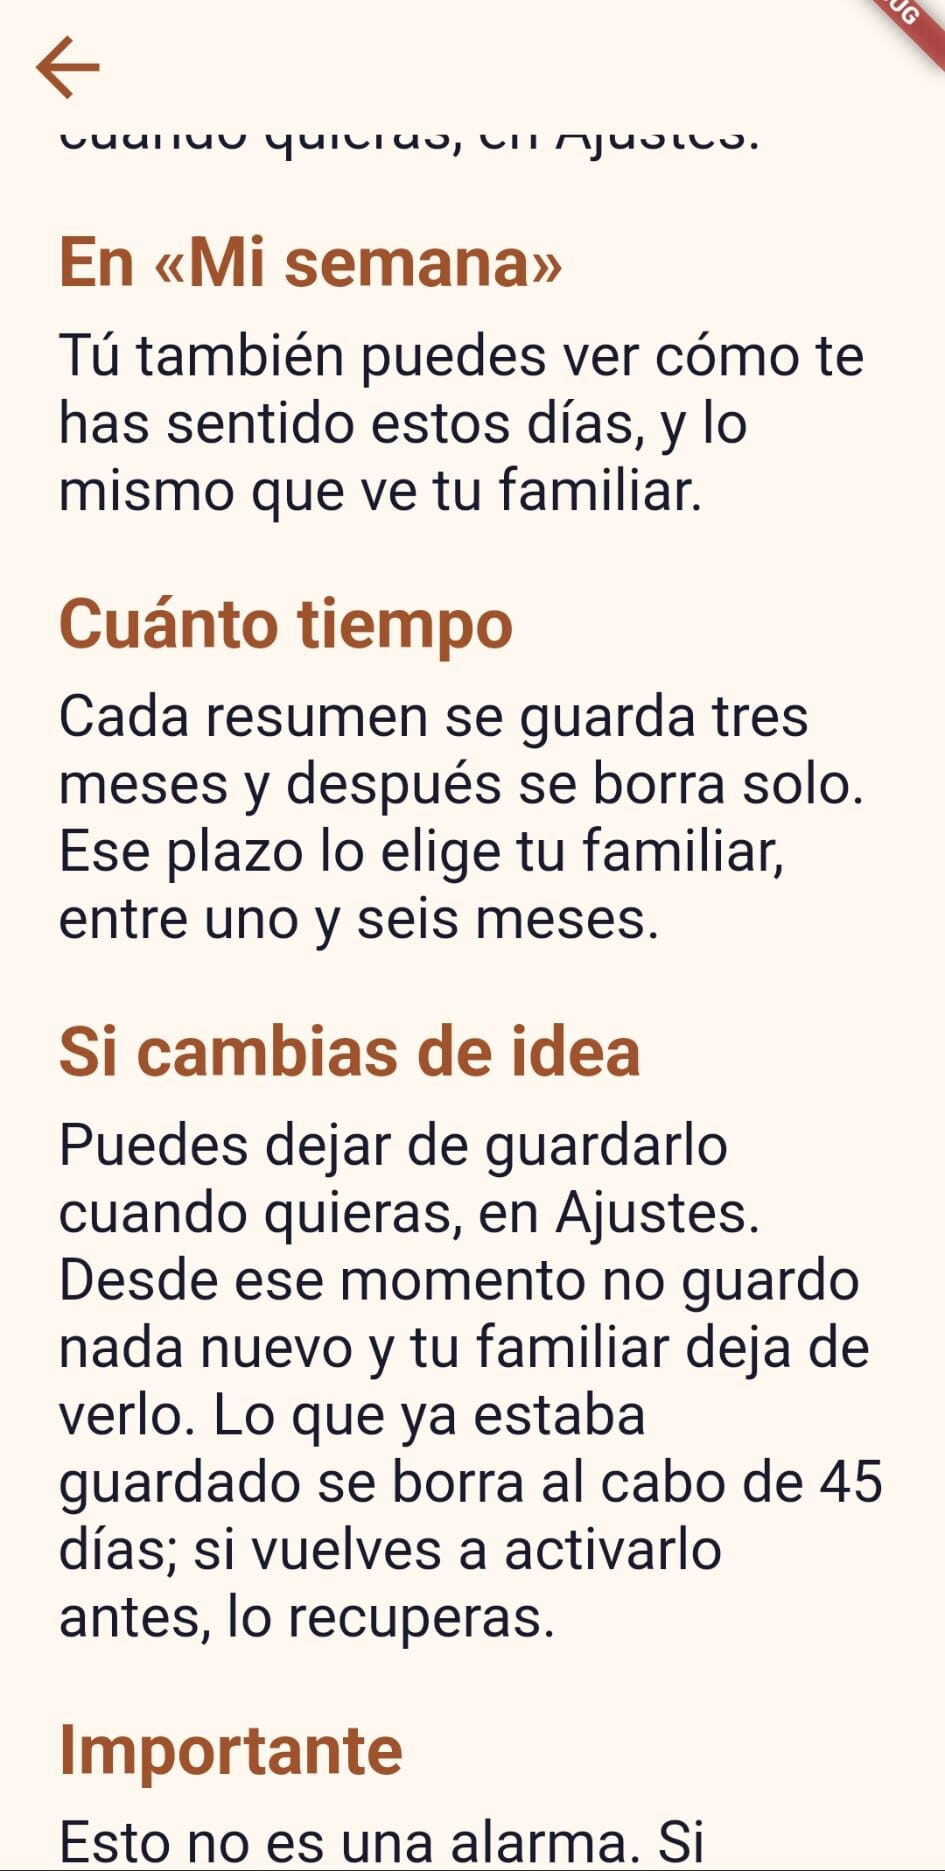
\includegraphics[width=\linewidth]{imagenes/manual/mayor-saber-mas}
    \caption{Saber más}
  \end{subfigure}\manualhueco
  \begin{subfigure}[t]{0.165\textwidth}\centering
    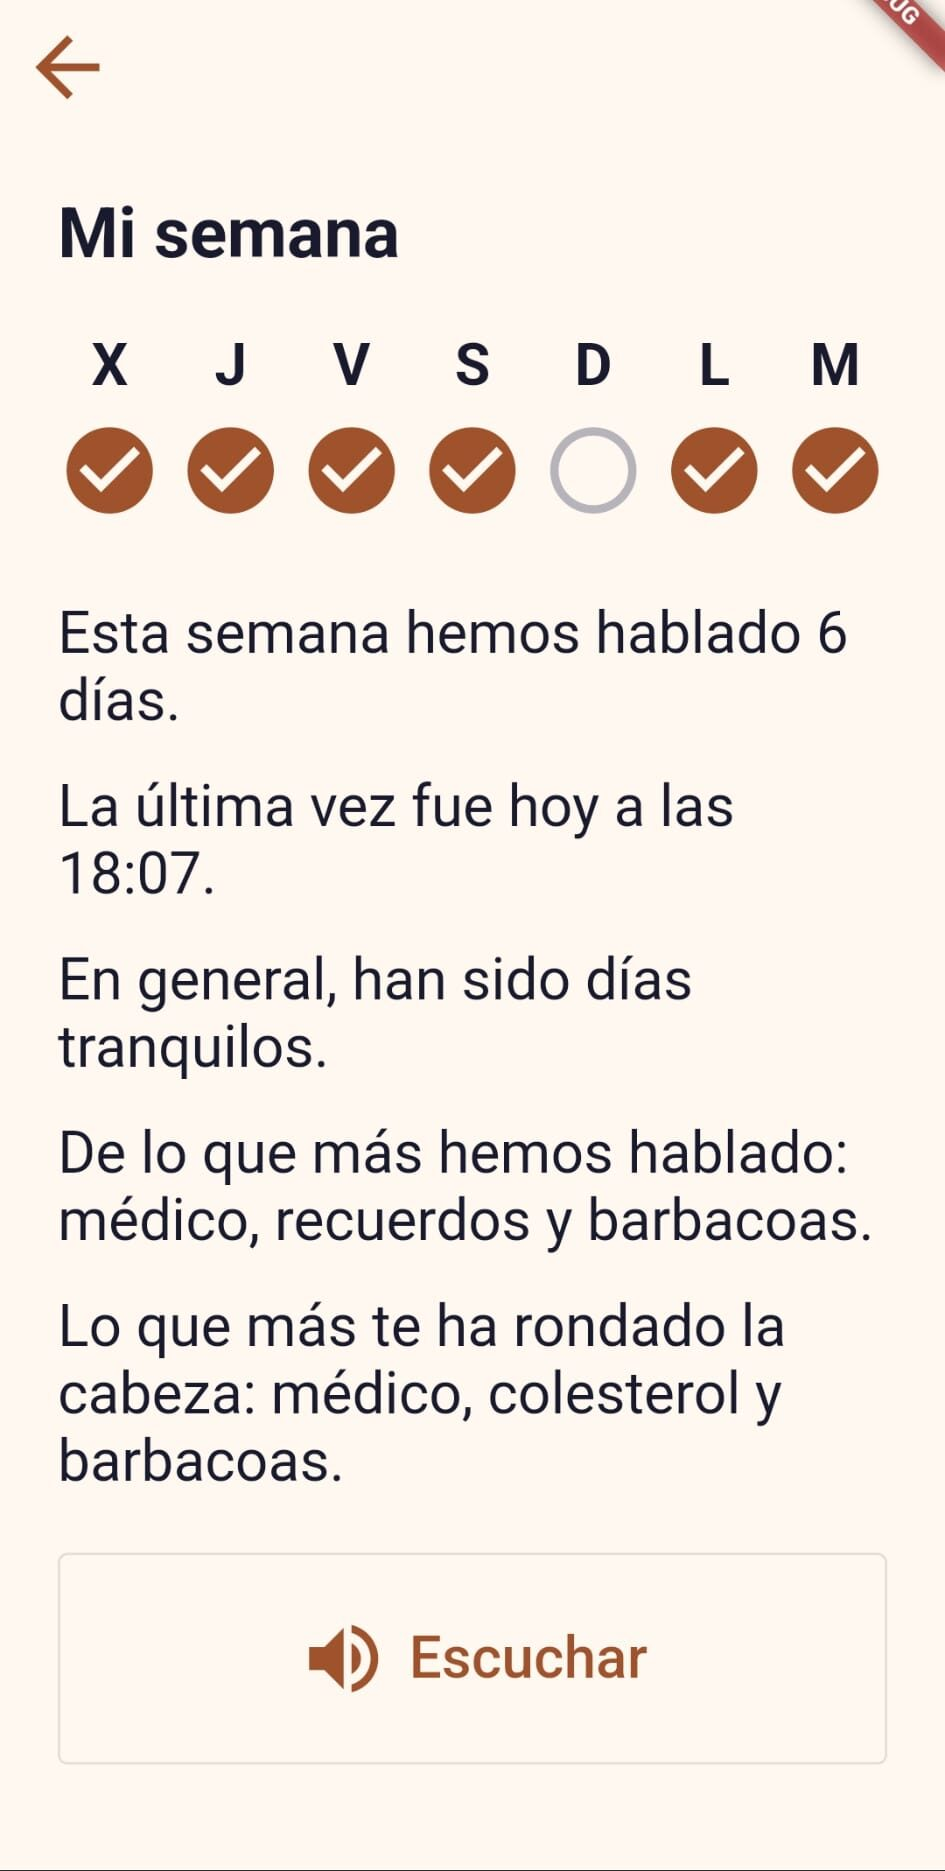
\includegraphics[width=\linewidth]{imagenes/manual/mayor-mi-semana}
    \caption{Mi semana}
  \end{subfigure}
  \caption{Lo que se guarda de las conversaciones y <<Mi semana>>.}
  \label{fig:manual-conversaciones}
\end{figure}

\begin{itemize}
  \item \textbf{Guardar mis conversaciones.} Activa o detiene el resumen. Si deja de guardarlas, desde ese momento no se guarda nada nuevo y su familiar deja de verlo. Lo que ya estaba guardado se borra pasado un tiempo, y la pantalla le indica la fecha; si vuelve a activarlo antes, lo recupera.
  \item \textbf{Qué ve mi familiar}, si está vinculado: nada (solo sabrá que guarda sus conversaciones), cómo se encuentra, o cómo se encuentra y de qué hablan. Lo elige usted y puede cambiarlo cuando quiera.
  \item \textbf{Cuándo termina una conversación} y \textbf{cuánto tiempo se guardan}, si usa la aplicación por su cuenta. Si está vinculado, estos plazos los elige su familiar.
\end{itemize}

<<Mi semana>>, en la pantalla principal, le cuenta con frases sencillas cómo ha ido su semana: qué días han conversado, cómo le ha notado el asistente, de qué han hablado más y lo que más le ha rondado la cabeza. <<Escuchar>> se lo lee en voz alta. Al final indica qué ve su familiar, con un botón para cambiarlo.

\section{El familiar}
\label{sec:manual-familiar}

\subsection{Crear la cuenta y vincularse}

En la primera pantalla de la aplicación, toque <<Soy el acompañante>> y después <<Crear una cuenta nueva>>, o <<Ya tengo una cuenta>> si ya se registró. El registro pide su nombre, un correo electrónico, una contraseña de al menos seis caracteres y su teléfono, que es el número al que llamará la persona mayor desde su botón de emergencia. Después escriba el código de cuatro caracteres que aparece en el móvil de la persona mayor cuando elige <<Vincular con mi familiar>> y pulse <<Vincular>> (\autoref{fig:manual-familiar}). Hecho esto, se abre el panel de control.

\begin{figure}[!htb]\centering
  \begin{subfigure}[t]{0.165\textwidth}\centering
    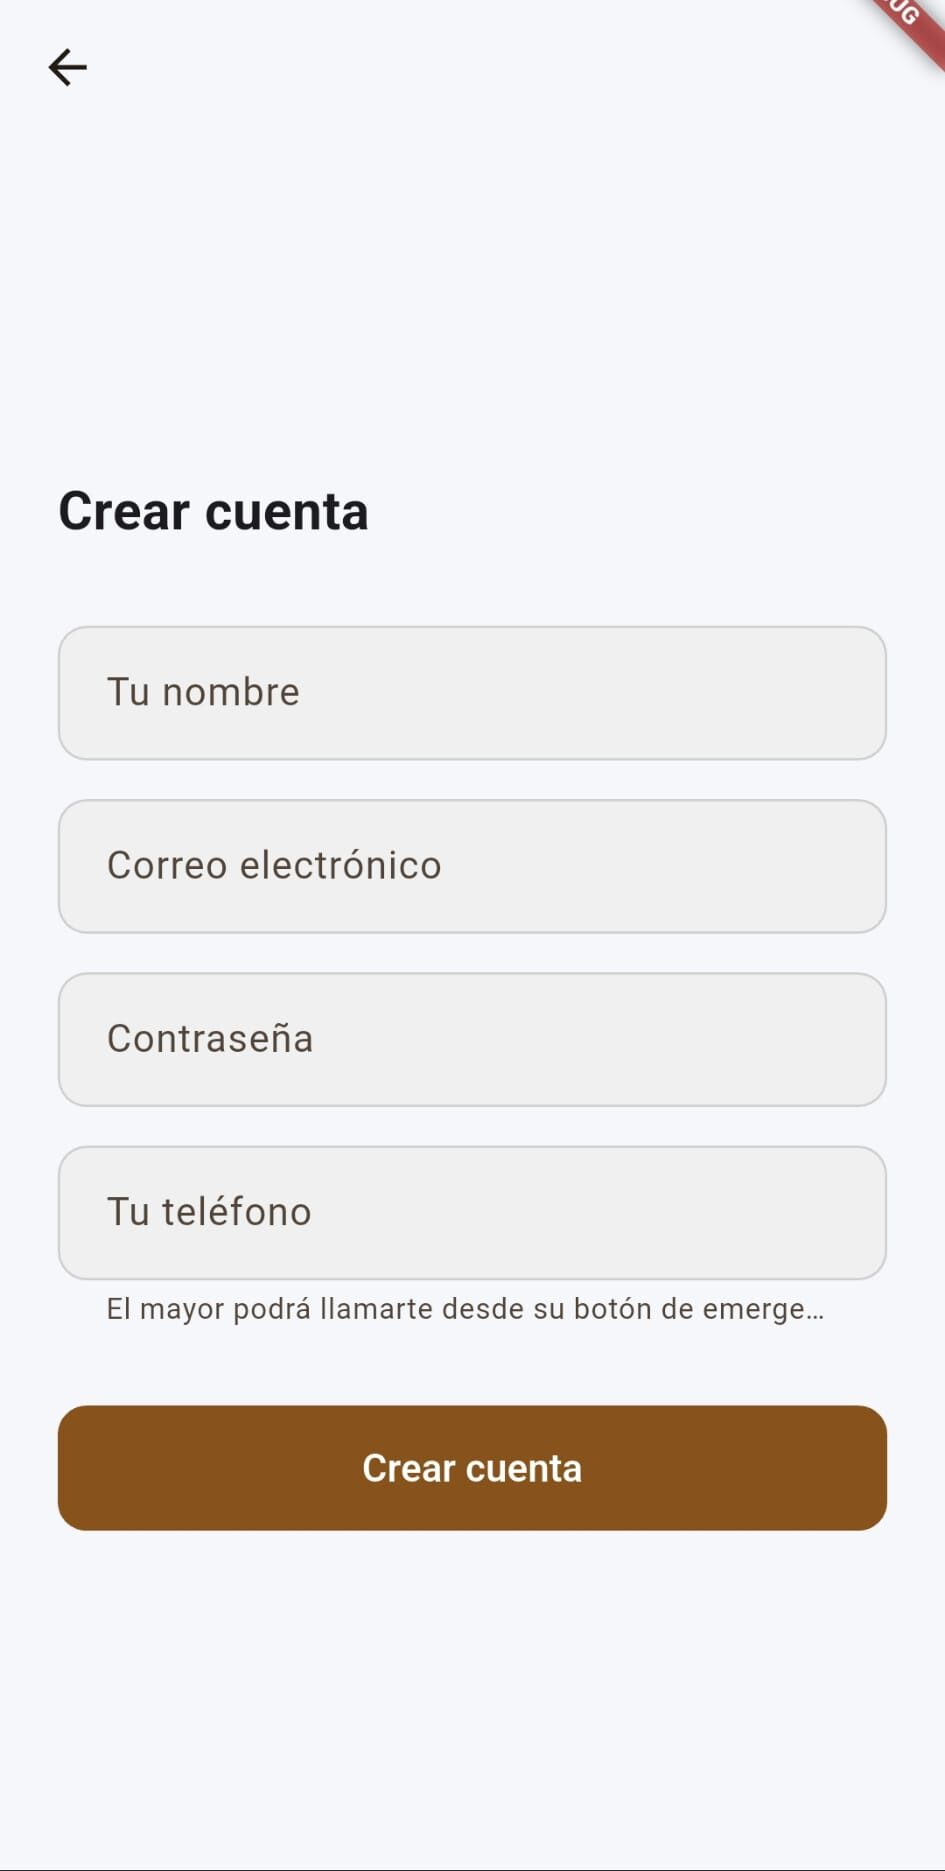
\includegraphics[width=\linewidth]{imagenes/manual/familiar-registro}
    \caption{Registro}
  \end{subfigure}\manualhueco
  \begin{subfigure}[t]{0.165\textwidth}\centering
    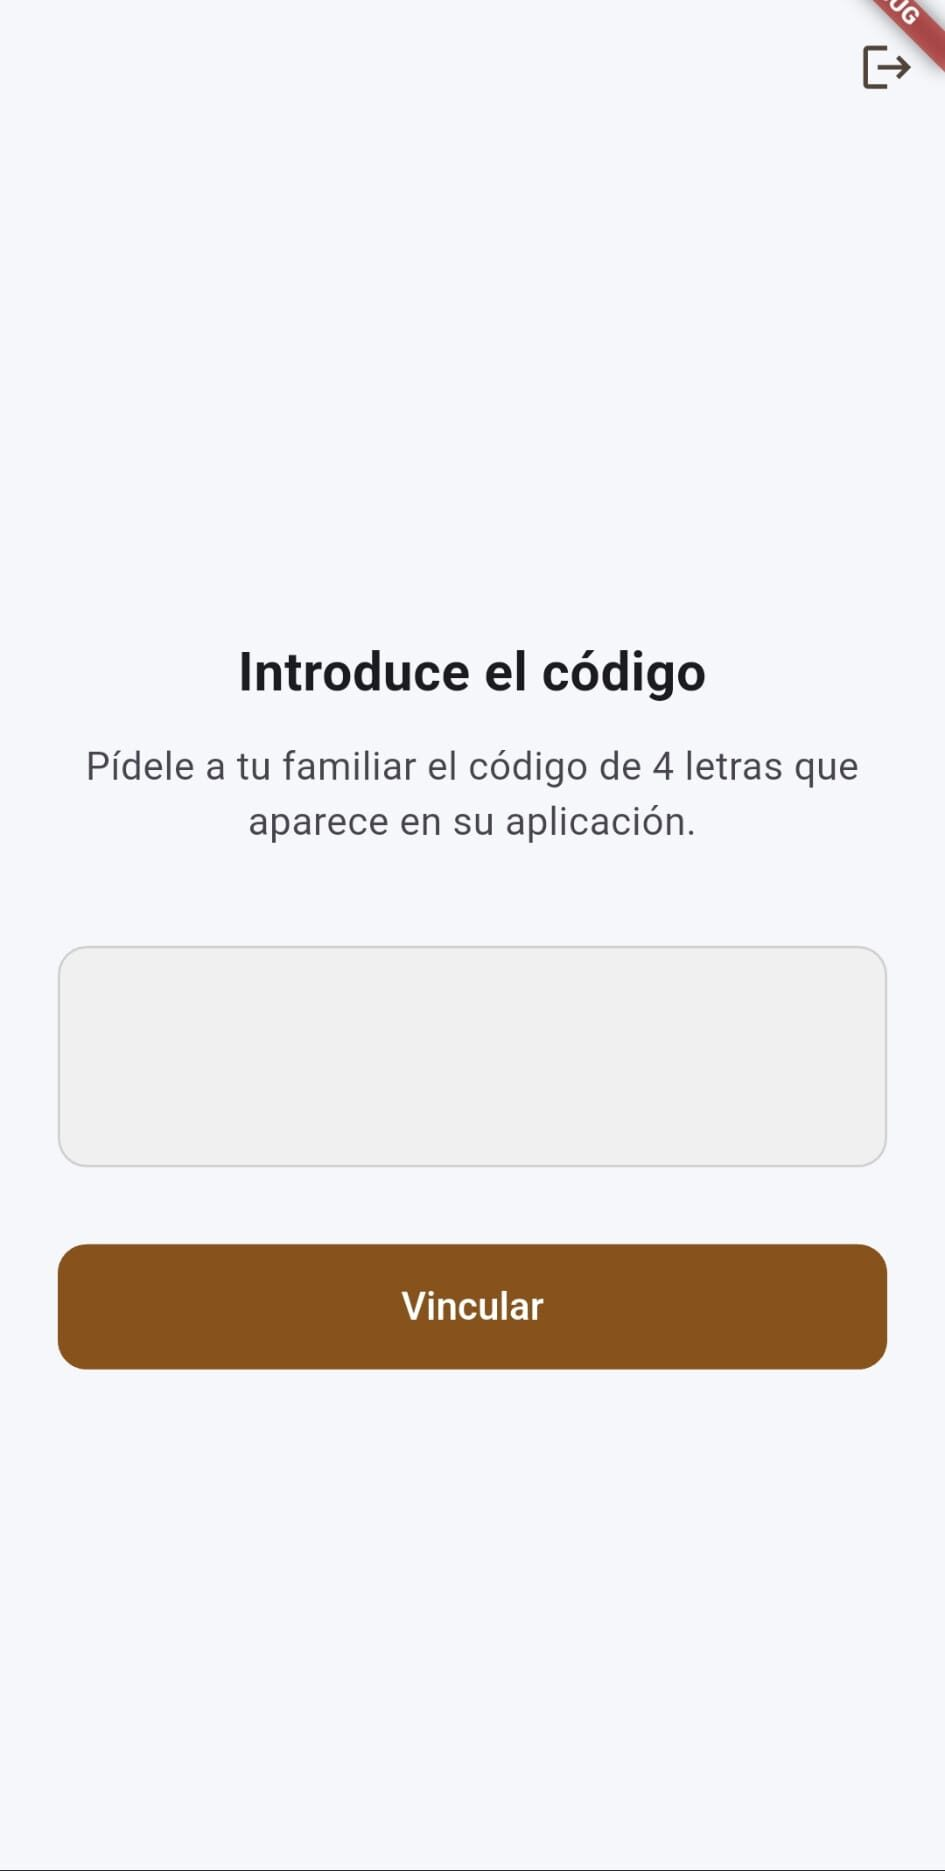
\includegraphics[width=\linewidth]{imagenes/manual/familiar-codigo}
    \caption{Código}
  \end{subfigure}\manualhueco
  \begin{subfigure}[t]{0.165\textwidth}\centering
    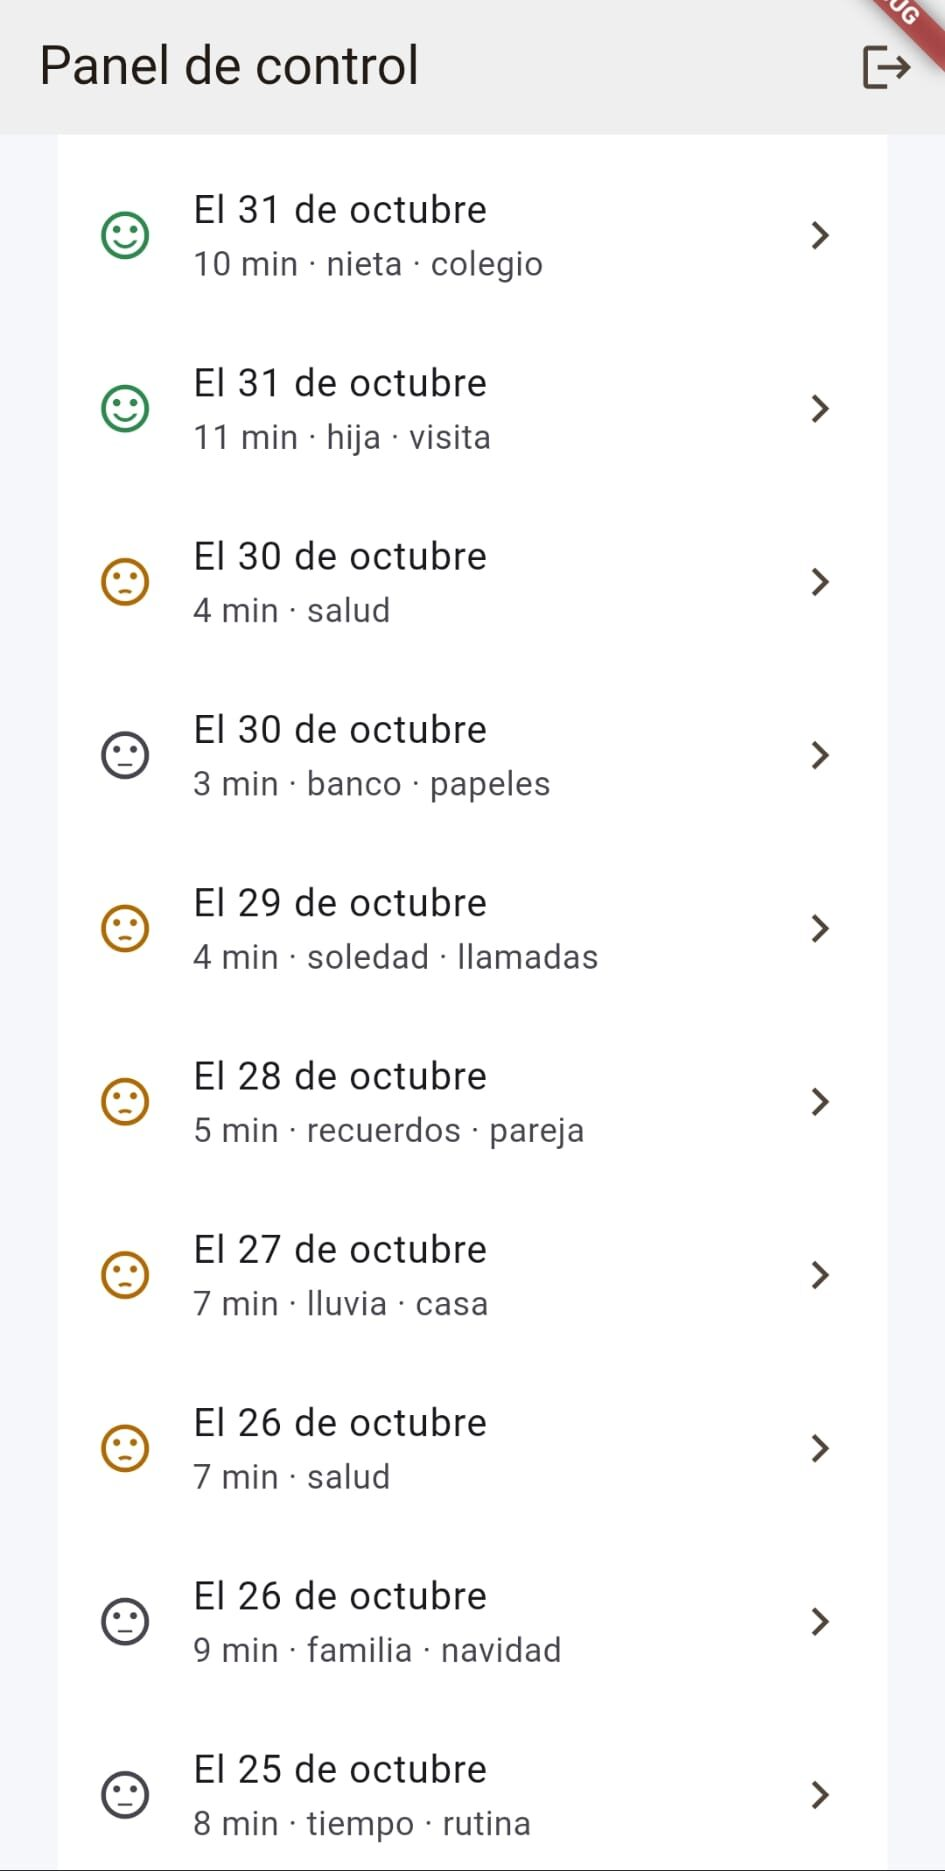
\includegraphics[width=\linewidth]{imagenes/manual/familiar-conversaciones}
    \caption{Lista}
  \end{subfigure}\manualhueco
  \begin{subfigure}[t]{0.165\textwidth}\centering
    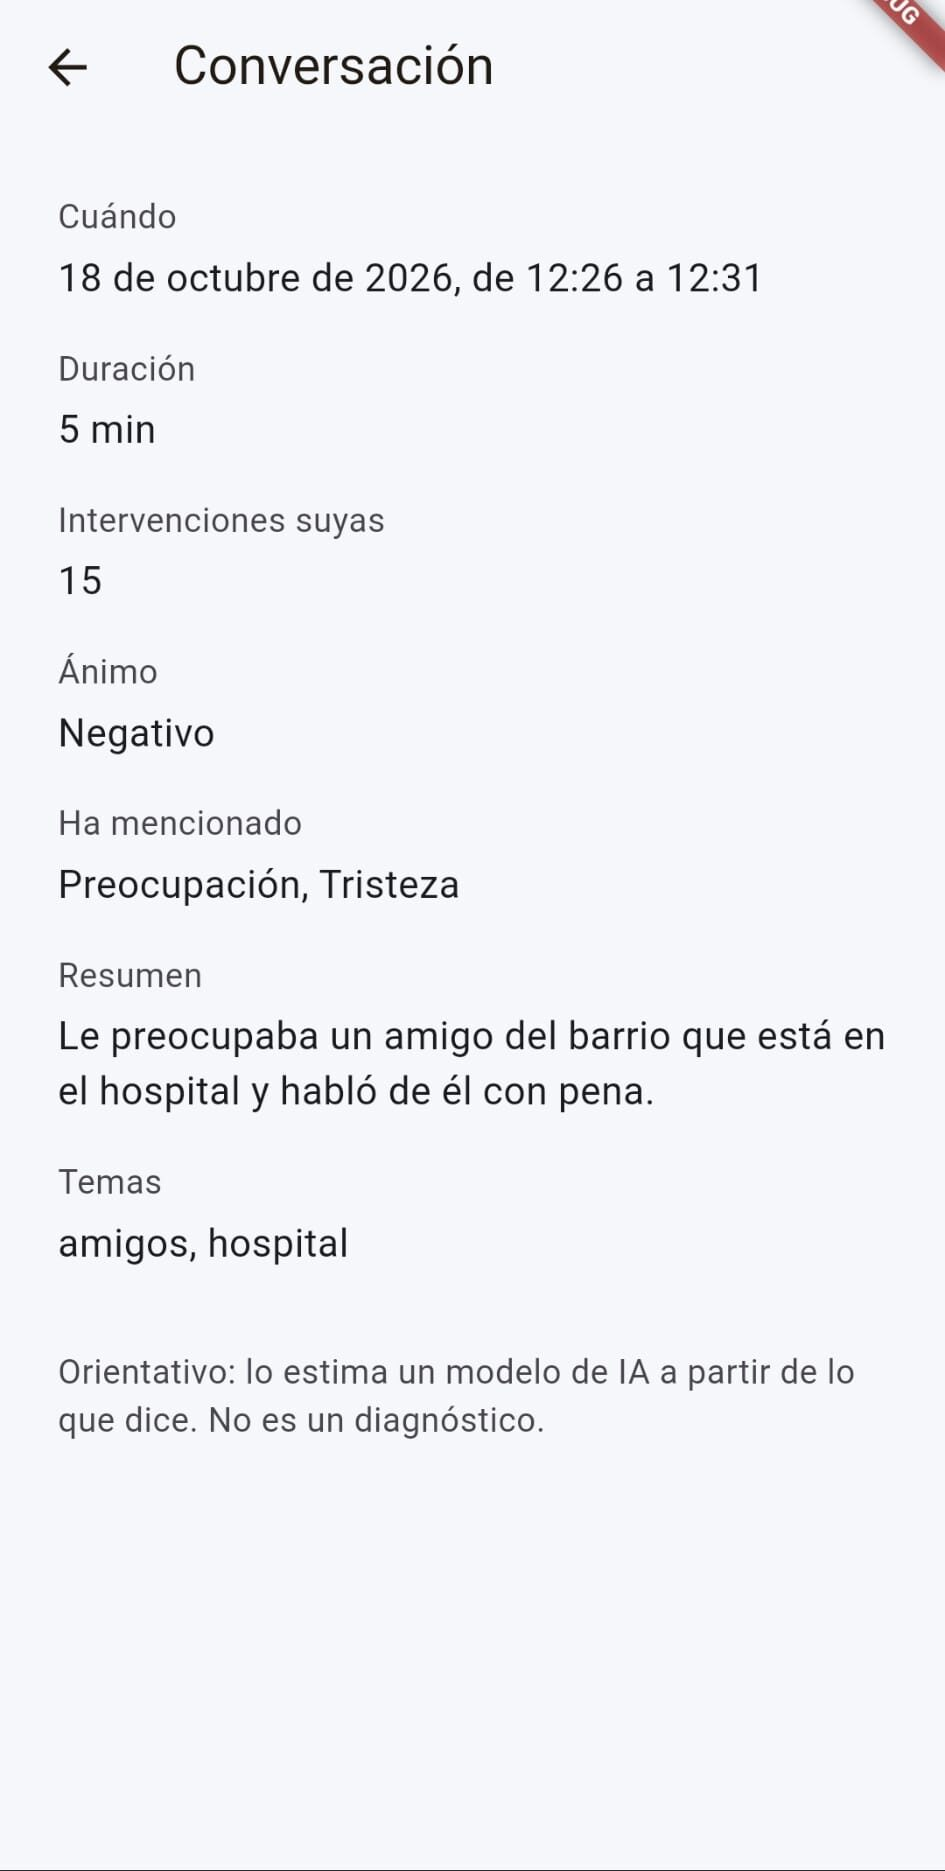
\includegraphics[width=\linewidth]{imagenes/manual/familiar-detalle}
    \caption{Detalle}
  \end{subfigure}\manualhueco
  \begin{subfigure}[t]{0.165\textwidth}\centering
    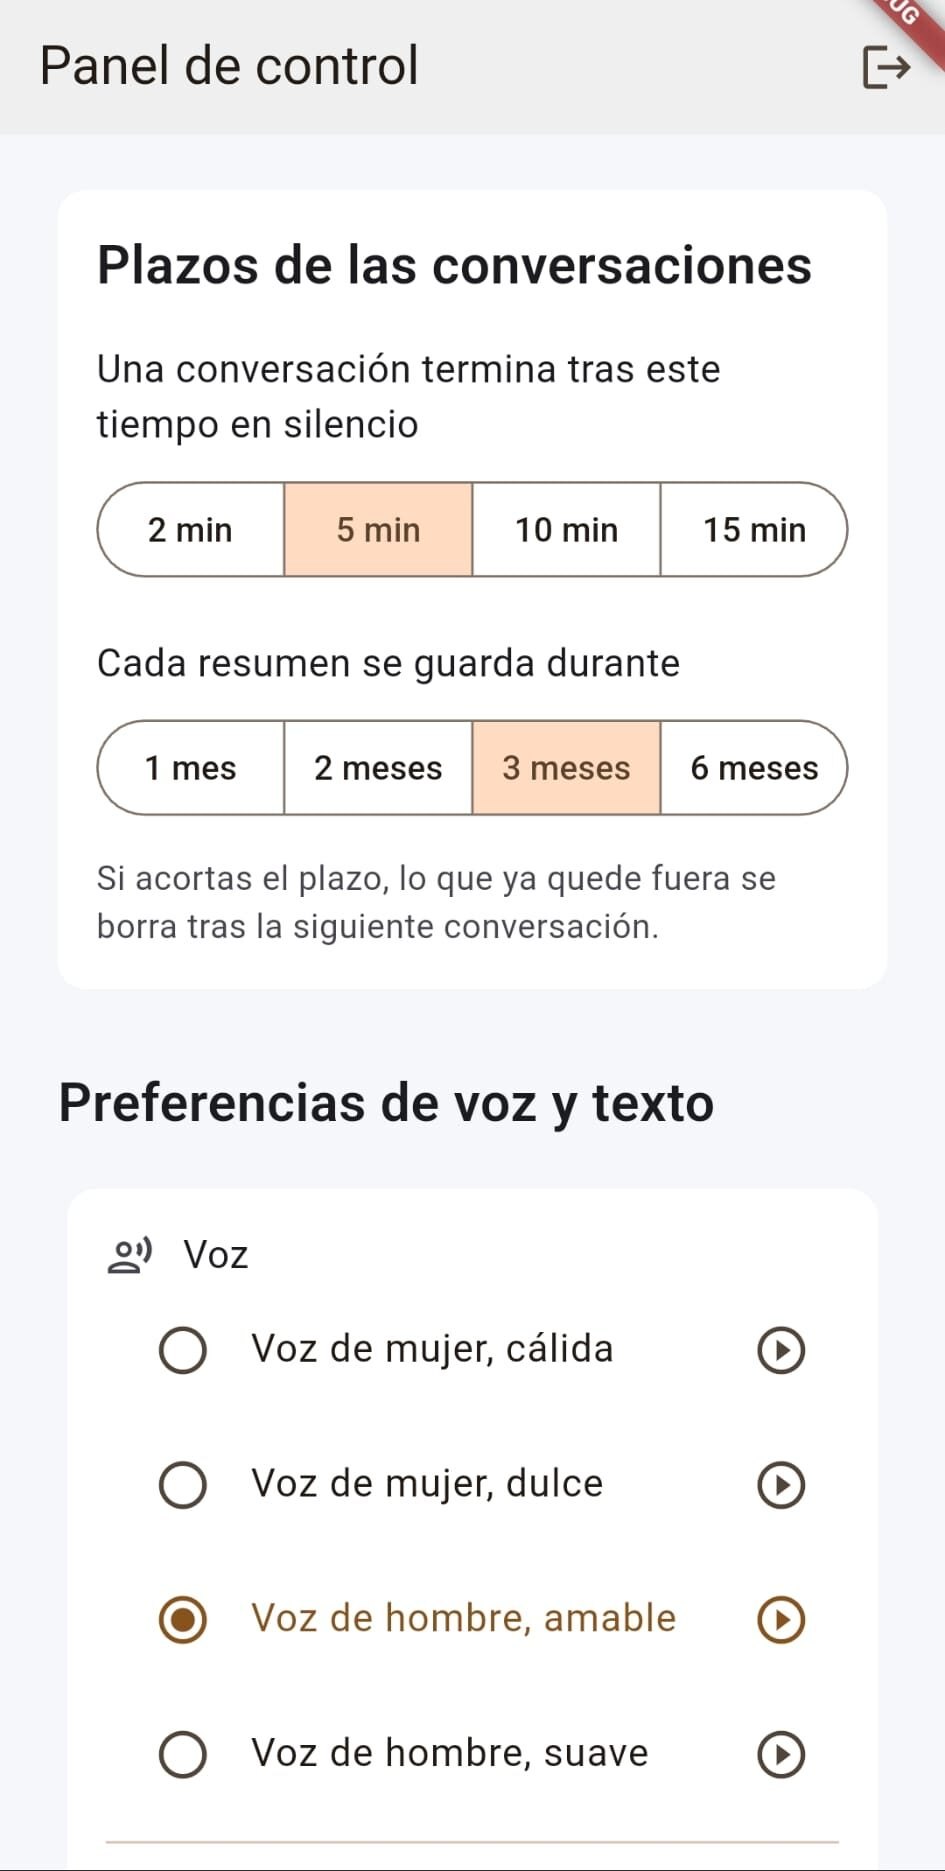
\includegraphics[width=\linewidth]{imagenes/manual/familiar-plazos}
    \caption{Plazos}
  \end{subfigure}
  \caption{Alta del familiar y otras pantallas del panel.}
  \label{fig:manual-familiar}
\end{figure}

\subsection{El panel de control}

\begin{figure}[!htb]\centering
  \begin{subfigure}[t]{0.27\textwidth}\centering
    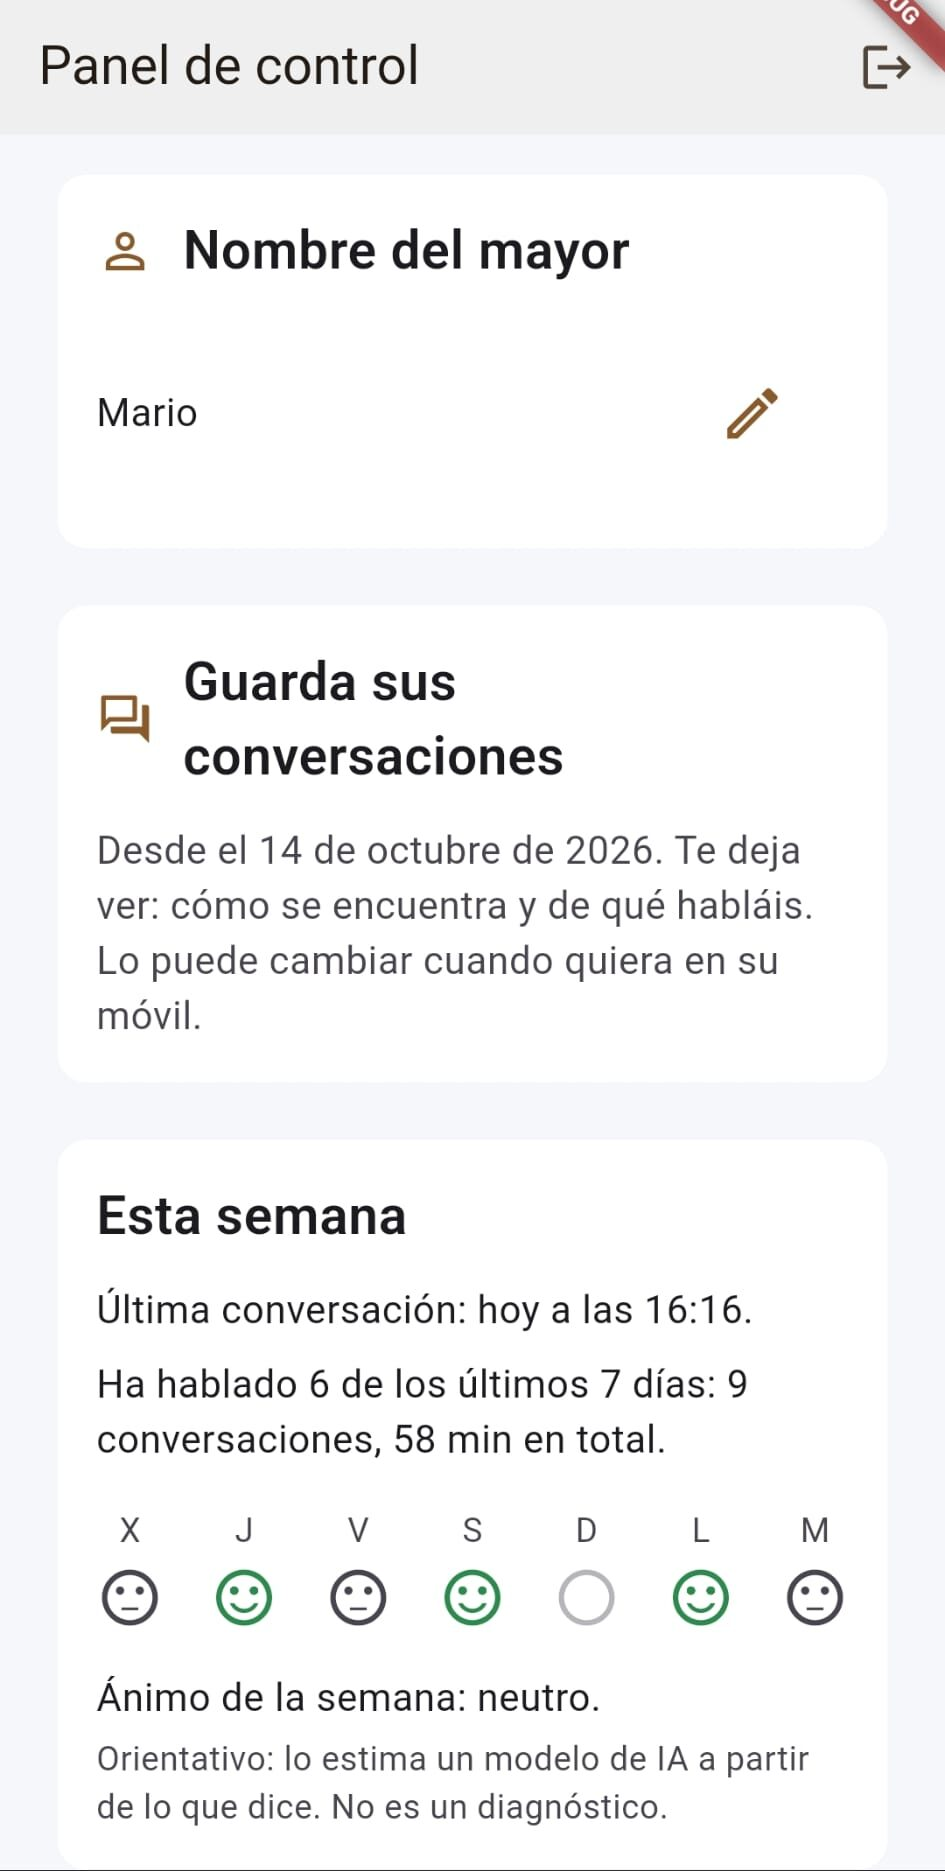
\includegraphics[width=\linewidth]{imagenes/manual/familiar-panel-semana}
    \caption{Esta semana}
  \end{subfigure}\hfill
  \begin{subfigure}[t]{0.27\textwidth}\centering
    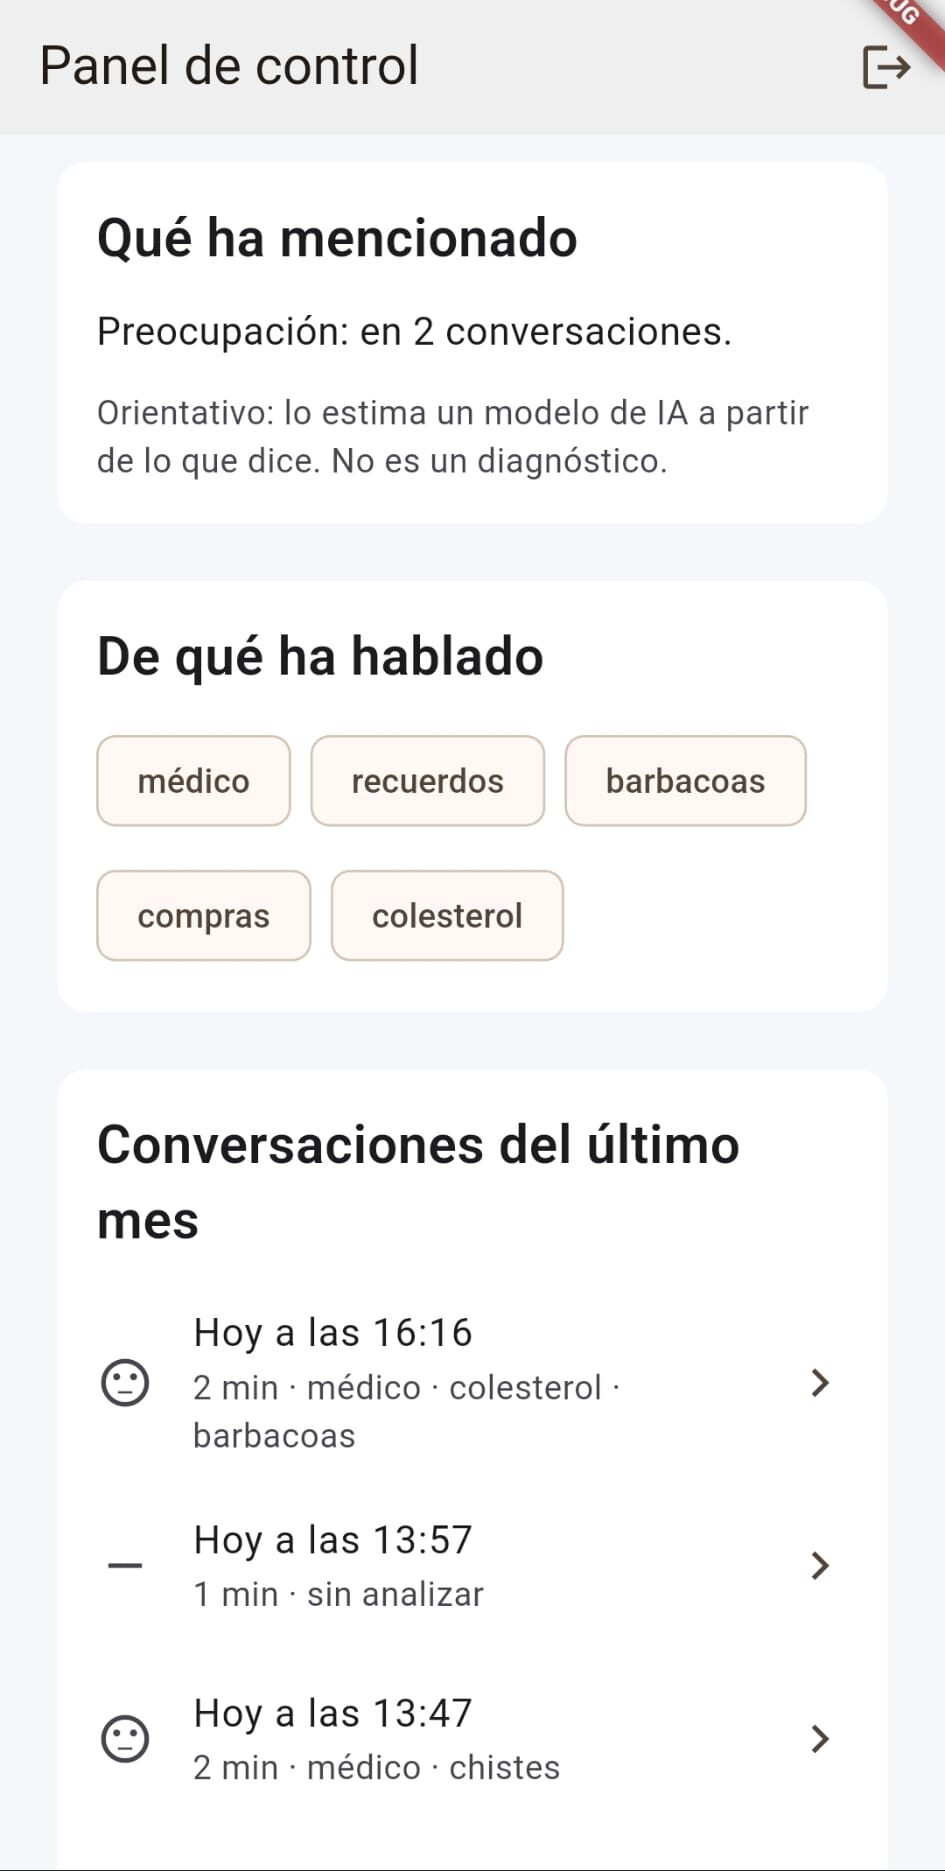
\includegraphics[width=\linewidth]{imagenes/manual/familiar-panel-temas}
    \caption{Señales y temas}
  \end{subfigure}\hfill
  \begin{subfigure}[t]{0.27\textwidth}\centering
    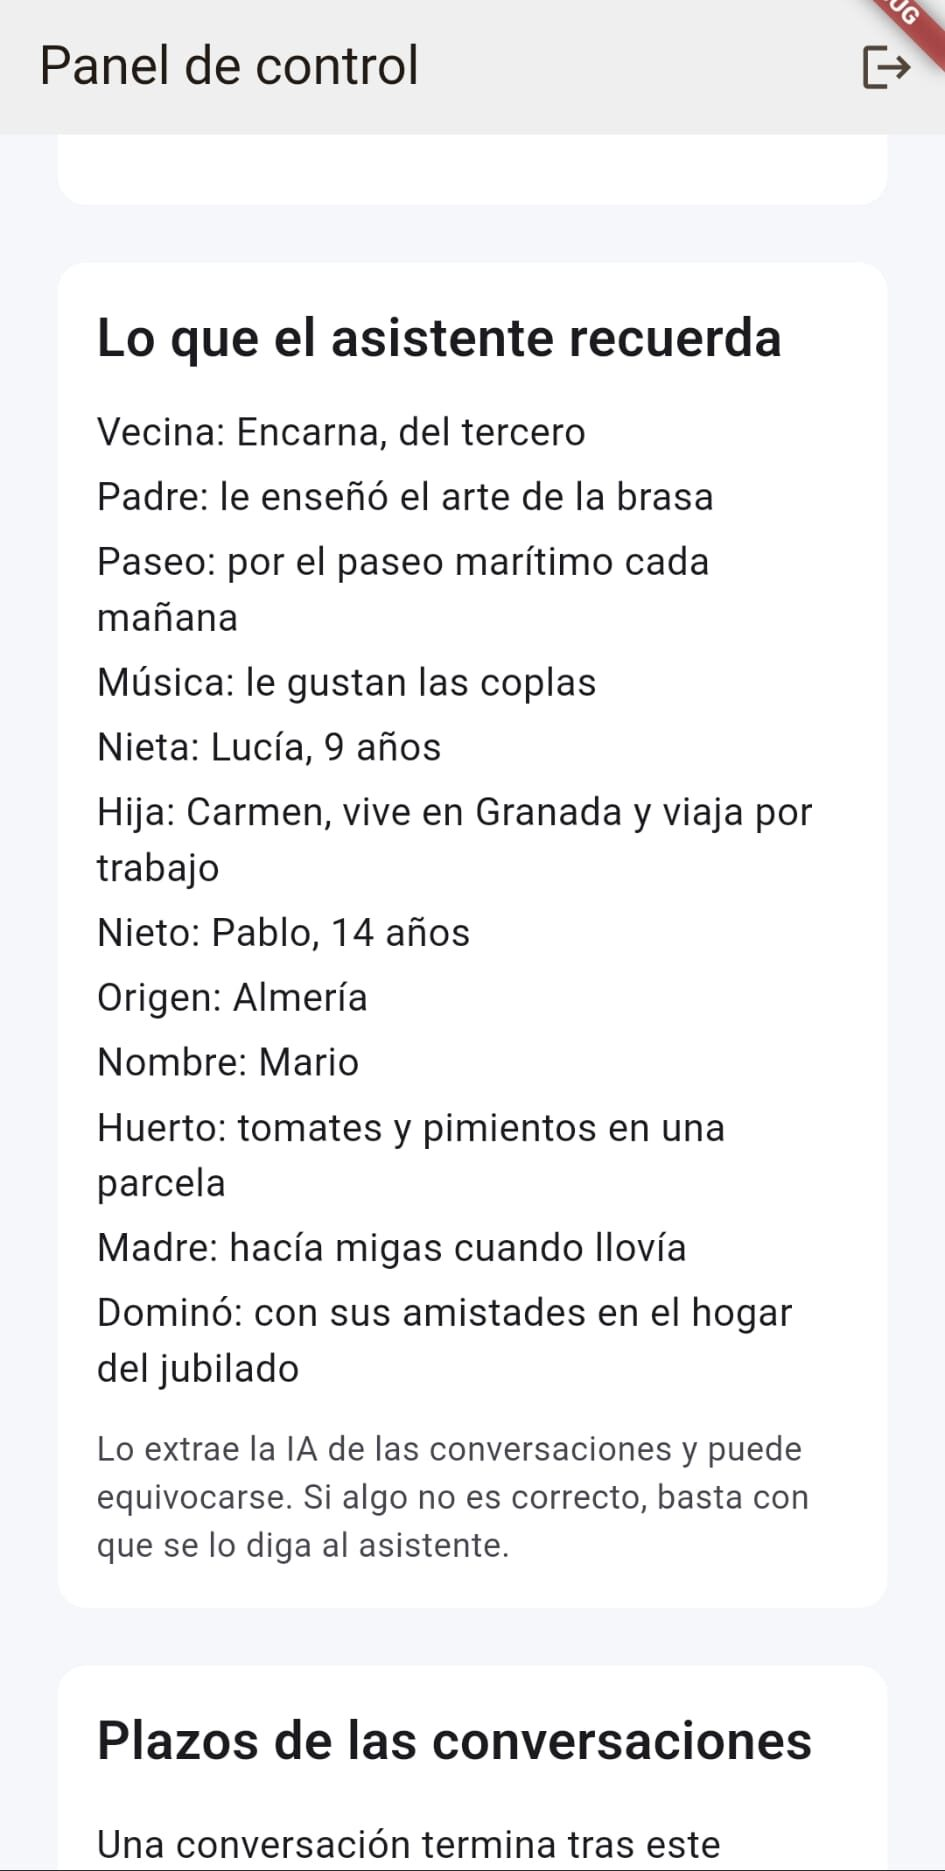
\includegraphics[width=\linewidth]{imagenes/manual/familiar-panel-recuerda}
    \caption{Lo que recuerda}
  \end{subfigure}
  \caption{Panel de control del familiar.}
  \label{fig:manual-panel}
\end{figure}

El panel es una sola pantalla que se recorre hacia abajo (\autoref{fig:manual-panel}). De arriba abajo muestra:

\begin{itemize}
  \item \textbf{Nombre del mayor.} El asistente lo aprende al conversar; el lápiz permite corregirlo.
  \item \textbf{Si guarda sus conversaciones}, desde cuándo y qué le deja ver. Solo la persona mayor puede cambiarlo, desde su móvil.
  \item \textbf{Esta semana.} Cuándo habló por última vez, cuántos días y cuánto tiempo, y una fila con los últimos siete días. La cara de cada día indica el ánimo (verde, positivo; gris, neutro; naranja, negativo), y el círculo vacío, que ese día no habló con el asistente.
  \item \textbf{Qué ha mencionado y de qué ha hablado.} Señales como preocupación, tristeza o soledad, con las conversaciones en que aparecen, y los temas que más se repiten.
  \item \textbf{Conversaciones del último mes.} Al tocar una se ve su detalle: cuándo fue, cuánto duró, el ánimo, lo que mencionó, un resumen breve y los temas. Las marcadas <<sin analizar>> no tienen resumen.
  \item \textbf{Lo que el asistente recuerda.} Lo que la persona mayor le ha contado de sí misma, como su familia o sus aficiones. Si algo no es correcto, basta con que ella se lo diga al asistente.
\end{itemize}

Si la persona mayor solo comparte <<Cómo me encuentro>>, no se muestran los temas, los resúmenes ni lo que recuerda el asistente, y en ningún caso se ve lo que dijo palabra por palabra. El ánimo y las señales los estima un modelo de inteligencia artificial: son orientativos, no un diagnóstico. Si en alguna conversación de la semana habló de hacerse daño o de no querer vivir, el panel lo avisa arriba, en rojo, junto a los teléfonos 112 y 024.

Al final del panel se fijan los plazos: cuánto silencio da por terminada una conversación (de 2 a 15 minutos) y cuánto se guarda cada resumen (de 1 a 6 meses); si acorta este último, lo que quede fuera se borra tras la siguiente conversación. En <<Preferencias de voz y texto>> elige la voz del asistente (el botón de reproducir la deja oír) y ajusta el volumen, la velocidad del habla y el tamaño del texto en el móvil de la persona mayor, que recibe los cambios al momento. Para cerrar sesión, use el icono de arriba a la derecha.

%%\input{apendices/paper/paper}
%\input{glosario/entradas_glosario}
% \addcontentsline{toc}{chapter}{Glosario}
% \printglossary

\end{document}
